\chapter{Systems} \label{chp:systems}
\epigraph{We must be clear that when it comes to atoms, language can be used only as in poetry.}{Niels Bohr, \cite{heisenberg_physics_1971}}
\begin{figure}[H]
	\centering
	%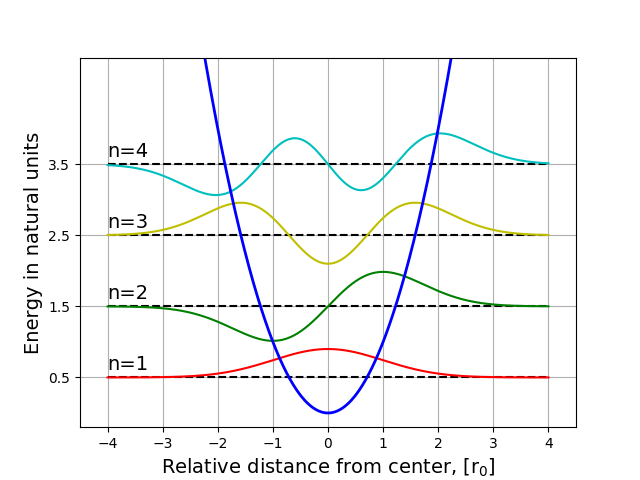
\includegraphics[scale=0.9]{Images/harmonicOscillator.png}
	% This file was created by matplotlib2tikz v0.7.4.
\begin{tikzpicture}

\begin{axis}[
%axis background/.style={fill=white!89.80392156862746!black},
axis line style={black},
tick align=outside,
tick pos=left,
tick align=outside,
tick pos=left,
x grid style={black},
xlabel={$r$},
xmajorgrids,
xmin=-4.5, xmax=4.5,
xtick={-4, -2, 0, 2, 4},
xticklabels={4, 2, 0, 2, 4},
ytick={0.5, 1.5, 2.5, 3.5},
xtick style={color=black},
y grid style={black},
ylabel={$E/\hbar\omega$},
ymajorgrids,
ymin=-0.2, ymax=5,
ytick style={color=black}
]
\addplot [semithick, black, dashed]
table {%
-4 0.5
-3.99199199199199 0.5
-3.98398398398398 0.5
-3.97597597597598 0.5
-3.96796796796797 0.5
-3.95995995995996 0.5
-3.95195195195195 0.5
-3.94394394394394 0.5
-3.93593593593594 0.5
-3.92792792792793 0.5
-3.91991991991992 0.5
-3.91191191191191 0.5
-3.9039039039039 0.5
-3.8958958958959 0.5
-3.88788788788789 0.5
-3.87987987987988 0.5
-3.87187187187187 0.5
-3.86386386386386 0.5
-3.85585585585586 0.5
-3.84784784784785 0.5
-3.83983983983984 0.5
-3.83183183183183 0.5
-3.82382382382382 0.5
-3.81581581581582 0.5
-3.80780780780781 0.5
-3.7997997997998 0.5
-3.79179179179179 0.5
-3.78378378378378 0.5
-3.77577577577578 0.5
-3.76776776776777 0.5
-3.75975975975976 0.5
-3.75175175175175 0.5
-3.74374374374374 0.5
-3.73573573573574 0.5
-3.72772772772773 0.5
-3.71971971971972 0.5
-3.71171171171171 0.5
-3.7037037037037 0.5
-3.6956956956957 0.5
-3.68768768768769 0.5
-3.67967967967968 0.5
-3.67167167167167 0.5
-3.66366366366366 0.5
-3.65565565565566 0.5
-3.64764764764765 0.5
-3.63963963963964 0.5
-3.63163163163163 0.5
-3.62362362362362 0.5
-3.61561561561562 0.5
-3.60760760760761 0.5
-3.5995995995996 0.5
-3.59159159159159 0.5
-3.58358358358358 0.5
-3.57557557557558 0.5
-3.56756756756757 0.5
-3.55955955955956 0.5
-3.55155155155155 0.5
-3.54354354354354 0.5
-3.53553553553554 0.5
-3.52752752752753 0.5
-3.51951951951952 0.5
-3.51151151151151 0.5
-3.5035035035035 0.5
-3.4954954954955 0.5
-3.48748748748749 0.5
-3.47947947947948 0.5
-3.47147147147147 0.5
-3.46346346346346 0.5
-3.45545545545546 0.5
-3.44744744744745 0.5
-3.43943943943944 0.5
-3.43143143143143 0.5
-3.42342342342342 0.5
-3.41541541541542 0.5
-3.40740740740741 0.5
-3.3993993993994 0.5
-3.39139139139139 0.5
-3.38338338338338 0.5
-3.37537537537538 0.5
-3.36736736736737 0.5
-3.35935935935936 0.5
-3.35135135135135 0.5
-3.34334334334334 0.5
-3.33533533533534 0.5
-3.32732732732733 0.5
-3.31931931931932 0.5
-3.31131131131131 0.5
-3.3033033033033 0.5
-3.2952952952953 0.5
-3.28728728728729 0.5
-3.27927927927928 0.5
-3.27127127127127 0.5
-3.26326326326326 0.5
-3.25525525525526 0.5
-3.24724724724725 0.5
-3.23923923923924 0.5
-3.23123123123123 0.5
-3.22322322322322 0.5
-3.21521521521522 0.5
-3.20720720720721 0.5
-3.1991991991992 0.5
-3.19119119119119 0.5
-3.18318318318318 0.5
-3.17517517517518 0.5
-3.16716716716717 0.5
-3.15915915915916 0.5
-3.15115115115115 0.5
-3.14314314314314 0.5
-3.13513513513514 0.5
-3.12712712712713 0.5
-3.11911911911912 0.5
-3.11111111111111 0.5
-3.1031031031031 0.5
-3.0950950950951 0.5
-3.08708708708709 0.5
-3.07907907907908 0.5
-3.07107107107107 0.5
-3.06306306306306 0.5
-3.05505505505506 0.5
-3.04704704704705 0.5
-3.03903903903904 0.5
-3.03103103103103 0.5
-3.02302302302302 0.5
-3.01501501501502 0.5
-3.00700700700701 0.5
-2.998998998999 0.5
-2.99099099099099 0.5
-2.98298298298298 0.5
-2.97497497497497 0.5
-2.96696696696697 0.5
-2.95895895895896 0.5
-2.95095095095095 0.5
-2.94294294294294 0.5
-2.93493493493493 0.5
-2.92692692692693 0.5
-2.91891891891892 0.5
-2.91091091091091 0.5
-2.9029029029029 0.5
-2.89489489489489 0.5
-2.88688688688689 0.5
-2.87887887887888 0.5
-2.87087087087087 0.5
-2.86286286286286 0.5
-2.85485485485485 0.5
-2.84684684684685 0.5
-2.83883883883884 0.5
-2.83083083083083 0.5
-2.82282282282282 0.5
-2.81481481481481 0.5
-2.80680680680681 0.5
-2.7987987987988 0.5
-2.79079079079079 0.5
-2.78278278278278 0.5
-2.77477477477477 0.5
-2.76676676676677 0.5
-2.75875875875876 0.5
-2.75075075075075 0.5
-2.74274274274274 0.5
-2.73473473473473 0.5
-2.72672672672673 0.5
-2.71871871871872 0.5
-2.71071071071071 0.5
-2.7027027027027 0.5
-2.69469469469469 0.5
-2.68668668668669 0.5
-2.67867867867868 0.5
-2.67067067067067 0.5
-2.66266266266266 0.5
-2.65465465465465 0.5
-2.64664664664665 0.5
-2.63863863863864 0.5
-2.63063063063063 0.5
-2.62262262262262 0.5
-2.61461461461461 0.5
-2.60660660660661 0.5
-2.5985985985986 0.5
-2.59059059059059 0.5
-2.58258258258258 0.5
-2.57457457457457 0.5
-2.56656656656657 0.5
-2.55855855855856 0.5
-2.55055055055055 0.5
-2.54254254254254 0.5
-2.53453453453453 0.5
-2.52652652652653 0.5
-2.51851851851852 0.5
-2.51051051051051 0.5
-2.5025025025025 0.5
-2.49449449449449 0.5
-2.48648648648649 0.5
-2.47847847847848 0.5
-2.47047047047047 0.5
-2.46246246246246 0.5
-2.45445445445445 0.5
-2.44644644644645 0.5
-2.43843843843844 0.5
-2.43043043043043 0.5
-2.42242242242242 0.5
-2.41441441441441 0.5
-2.40640640640641 0.5
-2.3983983983984 0.5
-2.39039039039039 0.5
-2.38238238238238 0.5
-2.37437437437437 0.5
-2.36636636636637 0.5
-2.35835835835836 0.5
-2.35035035035035 0.5
-2.34234234234234 0.5
-2.33433433433433 0.5
-2.32632632632633 0.5
-2.31831831831832 0.5
-2.31031031031031 0.5
-2.3023023023023 0.5
-2.29429429429429 0.5
-2.28628628628629 0.5
-2.27827827827828 0.5
-2.27027027027027 0.5
-2.26226226226226 0.5
-2.25425425425425 0.5
-2.24624624624625 0.5
-2.23823823823824 0.5
-2.23023023023023 0.5
-2.22222222222222 0.5
-2.21421421421421 0.5
-2.20620620620621 0.5
-2.1981981981982 0.5
-2.19019019019019 0.5
-2.18218218218218 0.5
-2.17417417417417 0.5
-2.16616616616617 0.5
-2.15815815815816 0.5
-2.15015015015015 0.5
-2.14214214214214 0.5
-2.13413413413413 0.5
-2.12612612612613 0.5
-2.11811811811812 0.5
-2.11011011011011 0.5
-2.1021021021021 0.5
-2.09409409409409 0.5
-2.08608608608609 0.5
-2.07807807807808 0.5
-2.07007007007007 0.5
-2.06206206206206 0.5
-2.05405405405405 0.5
-2.04604604604605 0.5
-2.03803803803804 0.5
-2.03003003003003 0.5
-2.02202202202202 0.5
-2.01401401401401 0.5
-2.00600600600601 0.5
-1.997997997998 0.5
-1.98998998998999 0.5
-1.98198198198198 0.5
-1.97397397397397 0.5
-1.96596596596597 0.5
-1.95795795795796 0.5
-1.94994994994995 0.5
-1.94194194194194 0.5
-1.93393393393393 0.5
-1.92592592592593 0.5
-1.91791791791792 0.5
-1.90990990990991 0.5
-1.9019019019019 0.5
-1.89389389389389 0.5
-1.88588588588589 0.5
-1.87787787787788 0.5
-1.86986986986987 0.5
-1.86186186186186 0.5
-1.85385385385385 0.5
-1.84584584584585 0.5
-1.83783783783784 0.5
-1.82982982982983 0.5
-1.82182182182182 0.5
-1.81381381381381 0.5
-1.80580580580581 0.5
-1.7977977977978 0.5
-1.78978978978979 0.5
-1.78178178178178 0.5
-1.77377377377377 0.5
-1.76576576576577 0.5
-1.75775775775776 0.5
-1.74974974974975 0.5
-1.74174174174174 0.5
-1.73373373373373 0.5
-1.72572572572573 0.5
-1.71771771771772 0.5
-1.70970970970971 0.5
-1.7017017017017 0.5
-1.69369369369369 0.5
-1.68568568568569 0.5
-1.67767767767768 0.5
-1.66966966966967 0.5
-1.66166166166166 0.5
-1.65365365365365 0.5
-1.64564564564565 0.5
-1.63763763763764 0.5
-1.62962962962963 0.5
-1.62162162162162 0.5
-1.61361361361361 0.5
-1.60560560560561 0.5
-1.5975975975976 0.5
-1.58958958958959 0.5
-1.58158158158158 0.5
-1.57357357357357 0.5
-1.56556556556557 0.5
-1.55755755755756 0.5
-1.54954954954955 0.5
-1.54154154154154 0.5
-1.53353353353353 0.5
-1.52552552552553 0.5
-1.51751751751752 0.5
-1.50950950950951 0.5
-1.5015015015015 0.5
-1.49349349349349 0.5
-1.48548548548549 0.5
-1.47747747747748 0.5
-1.46946946946947 0.5
-1.46146146146146 0.5
-1.45345345345345 0.5
-1.44544544544545 0.5
-1.43743743743744 0.5
-1.42942942942943 0.5
-1.42142142142142 0.5
-1.41341341341341 0.5
-1.40540540540541 0.5
-1.3973973973974 0.5
-1.38938938938939 0.5
-1.38138138138138 0.5
-1.37337337337337 0.5
-1.36536536536537 0.5
-1.35735735735736 0.5
-1.34934934934935 0.5
-1.34134134134134 0.5
-1.33333333333333 0.5
-1.32532532532533 0.5
-1.31731731731732 0.5
-1.30930930930931 0.5
-1.3013013013013 0.5
-1.29329329329329 0.5
-1.28528528528529 0.5
-1.27727727727728 0.5
-1.26926926926927 0.5
-1.26126126126126 0.5
-1.25325325325325 0.5
-1.24524524524525 0.5
-1.23723723723724 0.5
-1.22922922922923 0.5
-1.22122122122122 0.5
-1.21321321321321 0.5
-1.20520520520521 0.5
-1.1971971971972 0.5
-1.18918918918919 0.5
-1.18118118118118 0.5
-1.17317317317317 0.5
-1.16516516516517 0.5
-1.15715715715716 0.5
-1.14914914914915 0.5
-1.14114114114114 0.5
-1.13313313313313 0.5
-1.12512512512513 0.5
-1.11711711711712 0.5
-1.10910910910911 0.5
-1.1011011011011 0.5
-1.09309309309309 0.5
-1.08508508508509 0.5
-1.07707707707708 0.5
-1.06906906906907 0.5
-1.06106106106106 0.5
-1.05305305305305 0.5
-1.04504504504505 0.5
-1.03703703703704 0.5
-1.02902902902903 0.5
-1.02102102102102 0.5
-1.01301301301301 0.5
-1.00500500500501 0.5
-0.996996996996997 0.5
-0.988988988988989 0.5
-0.980980980980981 0.5
-0.972972972972973 0.5
-0.964964964964965 0.5
-0.956956956956957 0.5
-0.948948948948949 0.5
-0.940940940940941 0.5
-0.932932932932933 0.5
-0.924924924924925 0.5
-0.916916916916917 0.5
-0.908908908908909 0.5
-0.900900900900901 0.5
-0.892892892892893 0.5
-0.884884884884885 0.5
-0.876876876876877 0.5
-0.868868868868869 0.5
-0.860860860860861 0.5
-0.852852852852853 0.5
-0.844844844844845 0.5
-0.836836836836837 0.5
-0.828828828828829 0.5
-0.820820820820821 0.5
-0.812812812812813 0.5
-0.804804804804805 0.5
-0.796796796796797 0.5
-0.788788788788789 0.5
-0.780780780780781 0.5
-0.772772772772773 0.5
-0.764764764764765 0.5
-0.756756756756757 0.5
-0.748748748748749 0.5
-0.740740740740741 0.5
-0.732732732732733 0.5
-0.724724724724725 0.5
-0.716716716716717 0.5
-0.708708708708709 0.5
-0.700700700700701 0.5
-0.692692692692693 0.5
-0.684684684684685 0.5
-0.676676676676677 0.5
-0.668668668668669 0.5
-0.660660660660661 0.5
-0.652652652652653 0.5
-0.644644644644645 0.5
-0.636636636636636 0.5
-0.628628628628629 0.5
-0.620620620620621 0.5
-0.612612612612613 0.5
-0.604604604604605 0.5
-0.596596596596596 0.5
-0.588588588588589 0.5
-0.580580580580581 0.5
-0.572572572572573 0.5
-0.564564564564565 0.5
-0.556556556556556 0.5
-0.548548548548549 0.5
-0.54054054054054 0.5
-0.532532532532533 0.5
-0.524524524524525 0.5
-0.516516516516516 0.5
-0.508508508508509 0.5
-0.5005005005005 0.5
-0.492492492492492 0.5
-0.484484484484485 0.5
-0.476476476476476 0.5
-0.468468468468469 0.5
-0.46046046046046 0.5
-0.452452452452452 0.5
-0.444444444444445 0.5
-0.436436436436436 0.5
-0.428428428428429 0.5
-0.42042042042042 0.5
-0.412412412412412 0.5
-0.404404404404405 0.5
-0.396396396396396 0.5
-0.388388388388389 0.5
-0.38038038038038 0.5
-0.372372372372372 0.5
-0.364364364364365 0.5
-0.356356356356356 0.5
-0.348348348348348 0.5
-0.34034034034034 0.5
-0.332332332332332 0.5
-0.324324324324325 0.5
-0.316316316316316 0.5
-0.308308308308308 0.5
-0.3003003003003 0.5
-0.292292292292292 0.5
-0.284284284284285 0.5
-0.276276276276276 0.5
-0.268268268268268 0.5
-0.26026026026026 0.5
-0.252252252252252 0.5
-0.244244244244244 0.5
-0.236236236236236 0.5
-0.228228228228228 0.5
-0.22022022022022 0.5
-0.212212212212212 0.5
-0.204204204204204 0.5
-0.196196196196196 0.5
-0.188188188188188 0.5
-0.18018018018018 0.5
-0.172172172172172 0.5
-0.164164164164164 0.5
-0.156156156156156 0.5
-0.148148148148148 0.5
-0.14014014014014 0.5
-0.132132132132132 0.5
-0.124124124124124 0.5
-0.116116116116116 0.5
-0.108108108108108 0.5
-0.1001001001001 0.5
-0.0920920920920922 0.5
-0.084084084084084 0.5
-0.0760760760760761 0.5
-0.0680680680680683 0.5
-0.06006006006006 0.5
-0.0520520520520522 0.5
-0.0440440440440439 0.5
-0.0360360360360361 0.5
-0.0280280280280278 0.5
-0.02002002002002 0.5
-0.0120120120120122 0.5
-0.00400400400400391 0.5
0.00400400400400436 0.5
0.0120120120120122 0.5
0.02002002002002 0.5
0.0280280280280278 0.5
0.0360360360360357 0.5
0.0440440440440444 0.5
0.0520520520520522 0.5
0.06006006006006 0.5
0.0680680680680679 0.5
0.0760760760760757 0.5
0.0840840840840844 0.5
0.0920920920920922 0.5
0.1001001001001 0.5
0.108108108108108 0.5
0.116116116116116 0.5
0.124124124124124 0.5
0.132132132132132 0.5
0.14014014014014 0.5
0.148148148148148 0.5
0.156156156156156 0.5
0.164164164164164 0.5
0.172172172172172 0.5
0.18018018018018 0.5
0.188188188188188 0.5
0.196196196196196 0.5
0.204204204204204 0.5
0.212212212212212 0.5
0.22022022022022 0.5
0.228228228228228 0.5
0.236236236236236 0.5
0.244244244244245 0.5
0.252252252252252 0.5
0.26026026026026 0.5
0.268268268268268 0.5
0.276276276276276 0.5
0.284284284284285 0.5
0.292292292292292 0.5
0.3003003003003 0.5
0.308308308308308 0.5
0.316316316316316 0.5
0.324324324324325 0.5
0.332332332332332 0.5
0.34034034034034 0.5
0.348348348348348 0.5
0.356356356356356 0.5
0.364364364364365 0.5
0.372372372372372 0.5
0.38038038038038 0.5
0.388388388388388 0.5
0.396396396396397 0.5
0.404404404404405 0.5
0.412412412412412 0.5
0.42042042042042 0.5
0.428428428428428 0.5
0.436436436436437 0.5
0.444444444444445 0.5
0.452452452452452 0.5
0.46046046046046 0.5
0.468468468468468 0.5
0.476476476476477 0.5
0.484484484484485 0.5
0.492492492492492 0.5
0.5005005005005 0.5
0.508508508508508 0.5
0.516516516516517 0.5
0.524524524524525 0.5
0.532532532532533 0.5
0.54054054054054 0.5
0.548548548548548 0.5
0.556556556556557 0.5
0.564564564564565 0.5
0.572572572572573 0.5
0.58058058058058 0.5
0.588588588588588 0.5
0.596596596596597 0.5
0.604604604604605 0.5
0.612612612612613 0.5
0.62062062062062 0.5
0.628628628628628 0.5
0.636636636636637 0.5
0.644644644644645 0.5
0.652652652652653 0.5
0.66066066066066 0.5
0.668668668668668 0.5
0.676676676676677 0.5
0.684684684684685 0.5
0.692692692692693 0.5
0.7007007007007 0.5
0.708708708708708 0.5
0.716716716716717 0.5
0.724724724724725 0.5
0.732732732732733 0.5
0.74074074074074 0.5
0.748748748748748 0.5
0.756756756756757 0.5
0.764764764764765 0.5
0.772772772772773 0.5
0.780780780780781 0.5
0.788788788788788 0.5
0.796796796796797 0.5
0.804804804804805 0.5
0.812812812812813 0.5
0.820820820820821 0.5
0.828828828828828 0.5
0.836836836836837 0.5
0.844844844844845 0.5
0.852852852852853 0.5
0.860860860860861 0.5
0.868868868868869 0.5
0.876876876876877 0.5
0.884884884884885 0.5
0.892892892892893 0.5
0.900900900900901 0.5
0.908908908908909 0.5
0.916916916916917 0.5
0.924924924924925 0.5
0.932932932932933 0.5
0.940940940940941 0.5
0.948948948948949 0.5
0.956956956956957 0.5
0.964964964964965 0.5
0.972972972972973 0.5
0.980980980980981 0.5
0.988988988988989 0.5
0.996996996996997 0.5
1.00500500500501 0.5
1.01301301301301 0.5
1.02102102102102 0.5
1.02902902902903 0.5
1.03703703703704 0.5
1.04504504504505 0.5
1.05305305305305 0.5
1.06106106106106 0.5
1.06906906906907 0.5
1.07707707707708 0.5
1.08508508508509 0.5
1.09309309309309 0.5
1.1011011011011 0.5
1.10910910910911 0.5
1.11711711711712 0.5
1.12512512512513 0.5
1.13313313313313 0.5
1.14114114114114 0.5
1.14914914914915 0.5
1.15715715715716 0.5
1.16516516516517 0.5
1.17317317317317 0.5
1.18118118118118 0.5
1.18918918918919 0.5
1.1971971971972 0.5
1.20520520520521 0.5
1.21321321321321 0.5
1.22122122122122 0.5
1.22922922922923 0.5
1.23723723723724 0.5
1.24524524524525 0.5
1.25325325325325 0.5
1.26126126126126 0.5
1.26926926926927 0.5
1.27727727727728 0.5
1.28528528528529 0.5
1.29329329329329 0.5
1.3013013013013 0.5
1.30930930930931 0.5
1.31731731731732 0.5
1.32532532532533 0.5
1.33333333333333 0.5
1.34134134134134 0.5
1.34934934934935 0.5
1.35735735735736 0.5
1.36536536536537 0.5
1.37337337337337 0.5
1.38138138138138 0.5
1.38938938938939 0.5
1.3973973973974 0.5
1.40540540540541 0.5
1.41341341341341 0.5
1.42142142142142 0.5
1.42942942942943 0.5
1.43743743743744 0.5
1.44544544544545 0.5
1.45345345345345 0.5
1.46146146146146 0.5
1.46946946946947 0.5
1.47747747747748 0.5
1.48548548548549 0.5
1.49349349349349 0.5
1.5015015015015 0.5
1.50950950950951 0.5
1.51751751751752 0.5
1.52552552552553 0.5
1.53353353353353 0.5
1.54154154154154 0.5
1.54954954954955 0.5
1.55755755755756 0.5
1.56556556556557 0.5
1.57357357357357 0.5
1.58158158158158 0.5
1.58958958958959 0.5
1.5975975975976 0.5
1.60560560560561 0.5
1.61361361361361 0.5
1.62162162162162 0.5
1.62962962962963 0.5
1.63763763763764 0.5
1.64564564564565 0.5
1.65365365365365 0.5
1.66166166166166 0.5
1.66966966966967 0.5
1.67767767767768 0.5
1.68568568568569 0.5
1.69369369369369 0.5
1.7017017017017 0.5
1.70970970970971 0.5
1.71771771771772 0.5
1.72572572572573 0.5
1.73373373373373 0.5
1.74174174174174 0.5
1.74974974974975 0.5
1.75775775775776 0.5
1.76576576576577 0.5
1.77377377377377 0.5
1.78178178178178 0.5
1.78978978978979 0.5
1.7977977977978 0.5
1.80580580580581 0.5
1.81381381381381 0.5
1.82182182182182 0.5
1.82982982982983 0.5
1.83783783783784 0.5
1.84584584584585 0.5
1.85385385385385 0.5
1.86186186186186 0.5
1.86986986986987 0.5
1.87787787787788 0.5
1.88588588588589 0.5
1.89389389389389 0.5
1.9019019019019 0.5
1.90990990990991 0.5
1.91791791791792 0.5
1.92592592592593 0.5
1.93393393393393 0.5
1.94194194194194 0.5
1.94994994994995 0.5
1.95795795795796 0.5
1.96596596596597 0.5
1.97397397397397 0.5
1.98198198198198 0.5
1.98998998998999 0.5
1.997997997998 0.5
2.00600600600601 0.5
2.01401401401401 0.5
2.02202202202202 0.5
2.03003003003003 0.5
2.03803803803804 0.5
2.04604604604605 0.5
2.05405405405405 0.5
2.06206206206206 0.5
2.07007007007007 0.5
2.07807807807808 0.5
2.08608608608609 0.5
2.09409409409409 0.5
2.1021021021021 0.5
2.11011011011011 0.5
2.11811811811812 0.5
2.12612612612613 0.5
2.13413413413413 0.5
2.14214214214214 0.5
2.15015015015015 0.5
2.15815815815816 0.5
2.16616616616617 0.5
2.17417417417417 0.5
2.18218218218218 0.5
2.19019019019019 0.5
2.1981981981982 0.5
2.20620620620621 0.5
2.21421421421421 0.5
2.22222222222222 0.5
2.23023023023023 0.5
2.23823823823824 0.5
2.24624624624625 0.5
2.25425425425425 0.5
2.26226226226226 0.5
2.27027027027027 0.5
2.27827827827828 0.5
2.28628628628629 0.5
2.29429429429429 0.5
2.3023023023023 0.5
2.31031031031031 0.5
2.31831831831832 0.5
2.32632632632633 0.5
2.33433433433433 0.5
2.34234234234234 0.5
2.35035035035035 0.5
2.35835835835836 0.5
2.36636636636637 0.5
2.37437437437437 0.5
2.38238238238238 0.5
2.39039039039039 0.5
2.3983983983984 0.5
2.40640640640641 0.5
2.41441441441441 0.5
2.42242242242242 0.5
2.43043043043043 0.5
2.43843843843844 0.5
2.44644644644645 0.5
2.45445445445445 0.5
2.46246246246246 0.5
2.47047047047047 0.5
2.47847847847848 0.5
2.48648648648649 0.5
2.49449449449449 0.5
2.5025025025025 0.5
2.51051051051051 0.5
2.51851851851852 0.5
2.52652652652653 0.5
2.53453453453453 0.5
2.54254254254254 0.5
2.55055055055055 0.5
2.55855855855856 0.5
2.56656656656657 0.5
2.57457457457457 0.5
2.58258258258258 0.5
2.59059059059059 0.5
2.5985985985986 0.5
2.60660660660661 0.5
2.61461461461461 0.5
2.62262262262262 0.5
2.63063063063063 0.5
2.63863863863864 0.5
2.64664664664665 0.5
2.65465465465465 0.5
2.66266266266266 0.5
2.67067067067067 0.5
2.67867867867868 0.5
2.68668668668669 0.5
2.69469469469469 0.5
2.7027027027027 0.5
2.71071071071071 0.5
2.71871871871872 0.5
2.72672672672673 0.5
2.73473473473473 0.5
2.74274274274274 0.5
2.75075075075075 0.5
2.75875875875876 0.5
2.76676676676677 0.5
2.77477477477477 0.5
2.78278278278278 0.5
2.79079079079079 0.5
2.7987987987988 0.5
2.80680680680681 0.5
2.81481481481481 0.5
2.82282282282282 0.5
2.83083083083083 0.5
2.83883883883884 0.5
2.84684684684685 0.5
2.85485485485485 0.5
2.86286286286286 0.5
2.87087087087087 0.5
2.87887887887888 0.5
2.88688688688689 0.5
2.89489489489489 0.5
2.9029029029029 0.5
2.91091091091091 0.5
2.91891891891892 0.5
2.92692692692693 0.5
2.93493493493493 0.5
2.94294294294294 0.5
2.95095095095095 0.5
2.95895895895896 0.5
2.96696696696697 0.5
2.97497497497497 0.5
2.98298298298298 0.5
2.99099099099099 0.5
2.998998998999 0.5
3.00700700700701 0.5
3.01501501501502 0.5
3.02302302302302 0.5
3.03103103103103 0.5
3.03903903903904 0.5
3.04704704704705 0.5
3.05505505505506 0.5
3.06306306306306 0.5
3.07107107107107 0.5
3.07907907907908 0.5
3.08708708708709 0.5
3.0950950950951 0.5
3.1031031031031 0.5
3.11111111111111 0.5
3.11911911911912 0.5
3.12712712712713 0.5
3.13513513513514 0.5
3.14314314314314 0.5
3.15115115115115 0.5
3.15915915915916 0.5
3.16716716716717 0.5
3.17517517517518 0.5
3.18318318318318 0.5
3.19119119119119 0.5
3.1991991991992 0.5
3.20720720720721 0.5
3.21521521521522 0.5
3.22322322322322 0.5
3.23123123123123 0.5
3.23923923923924 0.5
3.24724724724725 0.5
3.25525525525526 0.5
3.26326326326326 0.5
3.27127127127127 0.5
3.27927927927928 0.5
3.28728728728729 0.5
3.2952952952953 0.5
3.3033033033033 0.5
3.31131131131131 0.5
3.31931931931932 0.5
3.32732732732733 0.5
3.33533533533534 0.5
3.34334334334334 0.5
3.35135135135135 0.5
3.35935935935936 0.5
3.36736736736737 0.5
3.37537537537538 0.5
3.38338338338338 0.5
3.39139139139139 0.5
3.3993993993994 0.5
3.40740740740741 0.5
3.41541541541542 0.5
3.42342342342342 0.5
3.43143143143143 0.5
3.43943943943944 0.5
3.44744744744745 0.5
3.45545545545546 0.5
3.46346346346346 0.5
3.47147147147147 0.5
3.47947947947948 0.5
3.48748748748749 0.5
3.4954954954955 0.5
3.5035035035035 0.5
3.51151151151151 0.5
3.51951951951952 0.5
3.52752752752753 0.5
3.53553553553554 0.5
3.54354354354354 0.5
3.55155155155155 0.5
3.55955955955956 0.5
3.56756756756757 0.5
3.57557557557558 0.5
3.58358358358358 0.5
3.59159159159159 0.5
3.5995995995996 0.5
3.60760760760761 0.5
3.61561561561562 0.5
3.62362362362362 0.5
3.63163163163163 0.5
3.63963963963964 0.5
3.64764764764765 0.5
3.65565565565566 0.5
3.66366366366366 0.5
3.67167167167167 0.5
3.67967967967968 0.5
3.68768768768769 0.5
3.6956956956957 0.5
3.7037037037037 0.5
3.71171171171171 0.5
3.71971971971972 0.5
3.72772772772773 0.5
3.73573573573574 0.5
3.74374374374374 0.5
3.75175175175175 0.5
3.75975975975976 0.5
3.76776776776777 0.5
3.77577577577578 0.5
3.78378378378378 0.5
3.79179179179179 0.5
3.7997997997998 0.5
3.80780780780781 0.5
3.81581581581582 0.5
3.82382382382382 0.5
3.83183183183183 0.5
3.83983983983984 0.5
3.84784784784785 0.5
3.85585585585586 0.5
3.86386386386386 0.5
3.87187187187187 0.5
3.87987987987988 0.5
3.88788788788789 0.5
3.8958958958959 0.5
3.9039039039039 0.5
3.91191191191191 0.5
3.91991991991992 0.5
3.92792792792793 0.5
3.93593593593594 0.5
3.94394394394394 0.5
3.95195195195195 0.5
3.95995995995996 0.5
3.96796796796797 0.5
3.97597597597598 0.5
3.98398398398398 0.5
3.99199199199199 0.5
4 0.5
};
\addplot [thick, color0]
table {%
-4 0.500134185051161
-3.99199199199199 0.500138548409832
-3.98398398398398 0.500143044480418
-3.97597597597598 0.500147676983603
-3.96796796796797 0.500152449734013
-3.95995995995996 0.500157366642269
-3.95195195195195 0.500162431717071
-3.94394394394394 0.500167649067314
-3.93593593593594 0.500173022904242
-3.92792792792793 0.500178557543638
-3.91991991991992 0.500184257408054
-3.91191191191191 0.500190127029069
-3.9039039039039 0.500196171049589
-3.8958958958959 0.500202394226187
-3.88788788788789 0.500208801431473
-3.87987987987988 0.500215397656508
-3.87187187187187 0.500222188013253
-3.86386386386386 0.500229177737055
-3.85585585585586 0.500236372189173
-3.84784784784785 0.500243776859346
-3.83983983983984 0.50025139736839
-3.83183183183183 0.500259239470843
-3.82382382382382 0.500267309057647
-3.81581581581582 0.500275612158868
-3.80780780780781 0.500284154946454
-3.7997997997998 0.500292943737036
-3.79179179179179 0.500301984994768
-3.78378378378378 0.500311285334202
-3.77577577577578 0.500320851523215
-3.76776776776777 0.50033069048596
-3.75975975975976 0.500340809305869
-3.75175175175175 0.500351215228693
-3.74374374374374 0.500361915665582
-3.73573573573574 0.500372918196203
-3.72772772772773 0.500384230571903
-3.71971971971972 0.500395860718907
-3.71171171171171 0.500407816741562
-3.7037037037037 0.500420106925616
-3.6956956956957 0.500432739741541
-3.68768768768769 0.500445723847895
-3.67967967967968 0.50045906809472
-3.67167167167167 0.500472781526987
-3.66366366366366 0.500486873388077
-3.65565565565566 0.500501353123298
-3.64764764764765 0.500516230383451
-3.63963963963964 0.500531515028423
-3.63163163163163 0.500547217130828
-3.62362362362362 0.500563346979685
-3.61561561561562 0.500579915084129
-3.60760760760761 0.500596932177168
-3.5995995995996 0.500614409219472
-3.59159159159159 0.500632357403198
-3.58358358358358 0.50065078815586
-3.57557557557558 0.500669713144229
-3.56756756756757 0.500689144278266
-3.55955955955956 0.5007090937151
-3.55155155155155 0.500729573863034
-3.54354354354354 0.500750597385586
-3.53553553553554 0.500772177205566
-3.52752752752753 0.500794326509187
-3.51951951951952 0.500817058750205
-3.51151151151151 0.500840387654094
-3.5035035035035 0.500864327222249
-3.4954954954955 0.500888891736227
-3.48748748748749 0.500914095762004
-3.47947947947948 0.500939954154279
-3.47147147147147 0.500966482060788
-3.46346346346346 0.500993694926657
-3.45545545545546 0.50102160849878
-3.44744744744745 0.501050238830214
-3.43943943943944 0.501079602284609
-3.43143143143143 0.501109715540654
-3.42342342342342 0.501140595596546
-3.41541541541542 0.501172259774486
-3.40740740740741 0.501204725725185
-3.3993993993994 0.501238011432397
-3.39139139139139 0.501272135217464
-3.38338338338338 0.501307115743881
-3.37537537537538 0.50134297202187
-3.36736736736737 0.501379723412978
-3.35935935935936 0.501417389634672
-3.35135135135135 0.501455990764958
-3.34334334334334 0.501495547247003
-3.33533533533534 0.50153607989376
-3.32732732732733 0.501577609892612
-3.31931931931932 0.501620158810002
-3.31131131131131 0.501663748596081
-3.3033033033033 0.501708401589352
-3.2952952952953 0.501754140521305
-3.28728728728729 0.501800988521064
-3.27927927927928 0.501848969120012
-3.27127127127127 0.501898106256427
-3.26326326326326 0.501948424280091
-3.25525525525526 0.501999947956906
-3.24724724724725 0.502052702473484
-3.23923923923924 0.502106713441724
-3.23123123123123 0.502162006903383
-3.22322322322322 0.502218609334608
-3.21521521521522 0.502276547650466
-3.20720720720721 0.502335849209435
-3.1991991991992 0.502396541817881
-3.19119119119119 0.502458653734492
-3.18318318318318 0.502522213674695
-3.17517517517518 0.502587250815029
-3.16716716716717 0.502653794797487
-3.15915915915916 0.502721875733817
-3.15115115115115 0.502791524209777
-3.14314314314314 0.502862771289357
-3.13513513513514 0.50293564851894
-3.12712712712713 0.503010187931424
-3.11911911911912 0.503086422050282
-3.11111111111111 0.503164383893572
-3.1031031031031 0.503244106977889
-3.0950950950951 0.503325625322249
-3.08708708708709 0.50340897345191
-3.07907907907908 0.503494186402132
-3.07107107107107 0.503581299721855
-3.06306306306306 0.503670349477308
-3.05505505505506 0.50376137225554
-3.04704704704705 0.503854405167869
-3.03903903903904 0.503949485853248
-3.03103103103103 0.504046652481539
-3.02302302302302 0.504145943756702
-3.01501501501502 0.504247398919882
-3.00700700700701 0.504351057752402
-2.998998998999 0.504456960578656
-2.99099099099099 0.504565148268889
-2.98298298298298 0.504675662241877
-2.97497497497497 0.504788544467485
-2.96696696696697 0.504903837469115
-2.95895895895896 0.505021584326029
-2.95095095095095 0.505141828675554
-2.94294294294294 0.505264614715149
-2.93493493493493 0.505389987204351
-2.92692692692693 0.505517991466574
-2.91891891891892 0.505648673390778
-2.91091091091091 0.505782079432989
-2.9029029029029 0.505918256617671
-2.89489489489489 0.506057252538947
-2.88688688688689 0.506199115361664
-2.87887887887888 0.506343893822299
-2.87087087087087 0.506491637229699
-2.86286286286286 0.506642395465651
-2.85485485485485 0.506796218985287
-2.84684684684685 0.506953158817304
-2.83883883883884 0.507113266564006
-2.83083083083083 0.507276594401161
-2.82282282282282 0.507443195077673
-2.81481481481481 0.507613121915051
-2.80680680680681 0.507786428806691
-2.7987987987988 0.507963170216947
-2.79079079079079 0.508143401180002
-2.78278278278278 0.508327177298524
-2.77477477477477 0.508514554742112
-2.76676676676677 0.508705590245519
-2.75875875875876 0.508900341106653
-2.75075075075075 0.509098865184351
-2.74274274274274 0.50930122089592
-2.73473473473473 0.509507467214445
-2.72672672672673 0.509717663665853
-2.71871871871872 0.509931870325737
-2.71071071071071 0.510150147815925
-2.7027027027027 0.510372557300803
-2.69469469469469 0.510599160483377
-2.68668668668669 0.510830019601076
-2.67867867867868 0.51106519742129
-2.67067067067067 0.511304757236637
-2.66266266266266 0.511548762859959
-2.65465465465465 0.511797278619037
-2.64664664664665 0.512050369351034
-2.63863863863864 0.51230810039664
-2.63063063063063 0.51257053759394
-2.62262262262262 0.512837747271982
-2.61461461461461 0.513109796244052
-2.60660660660661 0.513386751800649
-2.5985985985986 0.513668681702153
-2.59059059059059 0.513955654171188
-2.58258258258258 0.514247737884679
-2.57457457457457 0.514545001965581
-2.56656656656657 0.514847515974307
-2.55855855855856 0.515155349899824
-2.55055055055055 0.515468574150427
-2.54254254254254 0.515787259544187
-2.53453453453453 0.516111477299071
-2.52652652652653 0.516441299022719
-2.51851851851852 0.516776796701897
-2.51051051051051 0.517118042691604
-2.5025025025025 0.517465109703835
-2.49449449449449 0.517818070796006
-2.48648648648649 0.518176999359026
-2.47847847847848 0.518541969105024
-2.47047047047047 0.518913054054724
-2.46246246246246 0.51929032852446
-2.45445445445445 0.519673867112844
-2.44644644644645 0.520063744687069
-2.43843843843844 0.520460036368858
-2.43043043043043 0.520862817520047
-2.42242242242242 0.521272163727806
-2.41441441441441 0.521688150789501
-2.40640640640641 0.52211085469718
-2.3983983983984 0.522540351621702
-2.39039039039039 0.522976717896492
-2.38238238238238 0.523420030000932
-2.37437437437437 0.52387036454338
-2.36636636636637 0.524327798243817
-2.35835835835836 0.524792407916127
-2.35035035035035 0.525264270450008
-2.34234234234234 0.525743462792506
-2.33433433433433 0.526230061929185
-2.32632632632633 0.526724144864924
-2.31831831831832 0.527225788604341
-2.31031031031031 0.527735070131856
-2.3023023023023 0.528252066391376
-2.29429429429429 0.528776854265619
-2.28628628628629 0.529309510555072
-2.27827827827828 0.529850111956577
-2.27027027027027 0.530398735041561
-2.26226226226226 0.530955456233902
-2.25425425425425 0.531520351787435
-2.24624624624625 0.532093497763099
-2.23823823823824 0.532674970005729
-2.23023023023023 0.5332648441205
-2.22222222222222 0.533863195449012
-2.21421421421421 0.534470099045036
-2.20620620620621 0.535085629649913
-2.1981981981982 0.53570986166761
-2.19019019019019 0.536342869139442
-2.18218218218218 0.536984725718462
-2.17417417417417 0.537635504643515
-2.16616616616617 0.538295278712978
-2.15815815815816 0.538964120258167
-2.15015015015015 0.539642101116438
-2.14214214214214 0.540329292603971
-2.13413413413413 0.541025765488252
-2.12612612612613 0.541731589960251
-2.11811811811812 0.542446835606311
-2.11011011011011 0.543171571379737
-2.1021021021021 0.543905865572117
-2.09409409409409 0.544649785784352
-2.08608608608609 0.545403398897422
-2.07807807807808 0.546166771042894
-2.07007007007007 0.546939967573162
-2.06206206206206 0.547723053031446
-2.05405405405405 0.548516091121546
-2.04604604604605 0.549319144677364
-2.03803803803804 0.550132275632196
-2.03003003003003 0.550955544987809
-2.02202202202202 0.551789012783311
-2.01401401401401 0.552632738063809
-2.00600600600601 0.55348677884889
-1.997997997998 0.554351192100905
-1.98998998998999 0.555226033693089
-1.98198198198198 0.556111358377512
-1.97397397397397 0.557007219752874
-1.96596596596597 0.557913670232161
-1.95795795795796 0.558830761010163
-1.94994994994995 0.559758542030865
-1.94194194194194 0.560697061954736
-1.93393393393393 0.561646368125899
-1.92592592592593 0.562606506539228
-1.91791791791792 0.56357752180735
-1.90990990990991 0.564559457127588
-1.9019019019019 0.565552354248844
-1.89389389389389 0.566556253438438
-1.88588588588589 0.567571193448914
-1.87787787787788 0.568597211484827
-1.86986986986987 0.569634343169522
-1.86186186186186 0.570682622511919
-1.85385385385385 0.571742081873315
-1.84584584584585 0.572812751934218
-1.83783783783784 0.573894661661227
-1.82982982982983 0.574987838273968
-1.82182182182182 0.576092307212102
-1.81381381381381 0.577208092102423
-1.80580580580581 0.578335214726051
-1.7977977977978 0.57947369498574
-1.78978978978979 0.580623550873315
-1.78178178178178 0.581784798437253
-1.77377377377377 0.58295745175042
-1.76576576576577 0.584141522877981
-1.75775775775776 0.585337021845496
-1.74974974974975 0.586543956607217
-1.74174174174174 0.587762333014611
-1.73373373373373 0.588992154785101
-1.72572572572573 0.590233423471068
-1.71771771771772 0.591486138429111
-1.70970970970971 0.592750296789587
-1.7017017017017 0.594025893426443
-1.69369369369369 0.595312920927365
-1.68568568568569 0.59661136956425
-1.67767767767768 0.597921227264019
-1.66966966966967 0.599242479579787
-1.66166166166166 0.600575109662417
-1.65365365365365 0.601919098232451
-1.64564564564565 0.603274423552462
-1.63763763763764 0.604641061399814
-1.62962962962963 0.606018985039873
-1.62162162162162 0.607408165199669
-1.61361361361361 0.608808570042028
-1.60560560560561 0.610220165140195
-1.5975975975976 0.611642913452956
-1.58958958958959 0.613076775300287
-1.58158158158158 0.614521708339535
-1.57357357357357 0.615977667542151
-1.56556556556557 0.617444605170994
-1.55755755755756 0.618922470758217
-1.54954954954955 0.62041121108376
-1.54154154154154 0.621910770154447
-1.53353353353353 0.623421089183731
-1.52552552552553 0.624942106572076
-1.51751751751752 0.626473757888006
-1.50950950950951 0.628015975849834
-1.5015015015015 0.629568690308088
-1.49349349349349 0.63113182822864
-1.48548548548549 0.632705313676573
-1.47747747747748 0.63428906780077
-1.46946946946947 0.635883008819282
-1.46146146146146 0.63748705200544
-1.45345345345345 0.639101109674774
-1.44544544544545 0.640725091172717
-1.43743743743744 0.642358902863131
-1.42942942942943 0.644002448117651
-1.42142142142142 0.645655627305877
-1.41341341341341 0.647318337786421
-1.40540540540541 0.648990473898814
-1.3973973973974 0.650671926956306
-1.38938938938939 0.652362585239547
-1.38138138138138 0.654062333991184
-1.37337337337337 0.65577105541137
-1.36536536536537 0.657488628654211
-1.35735735735736 0.659214929825149
-1.34934934934935 0.660949831979298
-1.34134134134134 0.662693205120755
-1.33333333333333 0.664444916202875
-1.32532532532533 0.66620482912954
-1.31731731731732 0.667972804757422
-1.30930930930931 0.669748700899252
-1.3013013013013 0.67153237232811
-1.29329329329329 0.67332367078273
-1.28528528528529 0.67512244497385
-1.27727727727728 0.676928540591597
-1.26926926926927 0.678741800313927
-1.26126126126126 0.680562063816121
-1.25325325325325 0.682389167781342
-1.24524524524525 0.684222945912276
-1.23723723723724 0.686063228943837
-1.22922922922923 0.687909844656968
-1.22122122122122 0.689762617893524
-1.21321321321321 0.691621370572257
-1.20520520520521 0.693485921705899
-1.1971971971972 0.695356087419342
-1.18918918918919 0.697231680968938
-1.18118118118118 0.699112512762901
-1.17317317317317 0.700998390382827
-1.16516516516517 0.702889118606333
-1.15715715715716 0.704784499430803
-1.14914914914915 0.706684332098274
-1.14114114114114 0.708588413121419
-1.13313313313313 0.710496536310672
-1.12512512512513 0.712408492802458
-1.11711711711712 0.714324071088558
-1.10910910910911 0.716243057046578
-1.1011011011011 0.718165233971549
-1.09309309309309 0.720090382608638
-1.08508508508509 0.722018281186966
-1.07707707707708 0.723948705454546
-1.06906906906907 0.725881428714321
-1.06106106106106 0.727816221861305
-1.05305305305305 0.729752853420821
-1.04504504504505 0.73169108958783
-1.03703703703704 0.73363069426735
-1.02902902902903 0.735571429115948
-1.02102102102102 0.737513053584312
-1.01301301301301 0.739455324960882
-1.00500500500501 0.74139799841654
-0.996996996996997 0.74334082705035
-0.988988988988989 0.745283561936339
-0.980980980980981 0.7472259521713
-0.972972972972973 0.749167744923626
-0.964964964964965 0.751108685483145
-0.956956956956957 0.753048517311955
-0.948948948948949 0.754986982096241
-0.940940940940941 0.756923819799079
-0.932932932932933 0.758858768714181
-0.924924924924925 0.760791565520604
-0.916916916916917 0.762721945338383
-0.908908908908909 0.764649641785086
-0.900900900900901 0.766574387033274
-0.892892892892893 0.768495911868849
-0.884884884884885 0.770413945750269
-0.876876876876877 0.772328216868628
-0.868868868868869 0.774238452208571
-0.860860860860861 0.776144377610025
-0.852852852852853 0.778045717830743
-0.844844844844845 0.779942196609624
-0.836836836836837 0.781833536730808
-0.828828828828829 0.783719460088507
-0.820820820820821 0.785599687752568
-0.812812812812813 0.787473940034746
-0.804804804804805 0.789341936555654
-0.796796796796797 0.79120339631238
-0.788788788788789 0.793058037746751
-0.780780780780781 0.794905578814208
-0.772772772772773 0.796745737053285
-0.764764764764765 0.798578229655661
-0.756756756756757 0.800402773536761
-0.748748748748749 0.802219085406888
-0.740740740740741 0.80402688184285
-0.732732732732733 0.805825879360075
-0.724724724724725 0.807615794485176
-0.716716716716717 0.809396343828938
-0.708708708708709 0.811167244159718
-0.700700700700701 0.812928212477211
-0.692692692692693 0.814678966086577
-0.684684684684685 0.816419222672882
-0.676676676676677 0.818148700375839
-0.668668668668669 0.819867117864823
-0.660660660660661 0.821574194414123
-0.652652652652653 0.823269649978406
-0.644644644644645 0.824953205268379
-0.636636636636636 0.826624581826592
-0.628628628628629 0.82828350210339
-0.620620620620621 0.829929689532948
-0.612612612612613 0.831562868609395
-0.604604604604605 0.833182764962965
-0.596596596596596 0.834789105436179
-0.588588588588589 0.836381618159997
-0.580580580580581 0.837960032629937
-0.572572572572573 0.839524079782111
-0.564564564564565 0.841073492069166
-0.556556556556556 0.842608003536083
-0.548548548548549 0.844127349895818
-0.54054054054054 0.845631268604747
-0.532532532532533 0.847119498937894
-0.524524524524525 0.848591782063893
-0.516516516516516 0.850047861119682
-0.508508508508509 0.851487481284871
-0.5005005005005 0.852910389855775
-0.492492492492492 0.85431633631907
-0.484484484484485 0.855705072425046
-0.476476476476476 0.857076352260429
-0.468468468468469 0.85842993232074
-0.46046046046046 0.859765571582154
-0.452452452452452 0.861083031572851
-0.444444444444445 0.862382076443804
-0.436436436436436 0.863662473038987
-0.428428428428429 0.864923990964981
-0.42042042042042 0.866166402659931
-0.412412412412412 0.867389483461838
-0.404404404404405 0.868593011676162
-0.396396396396396 0.869776768642686
-0.388388388388389 0.870940538801638
-0.38038038038038 0.872084109759029
-0.372372372372372 0.873207272351178
-0.364364364364365 0.874309820708405
-0.356356356356356 0.875391552317859
-0.348348348348348 0.876452268085459
-0.34034034034034 0.87749177239691
-0.332332332332332 0.878509873177785
-0.324324324324325 0.879506381952634
-0.316316316316316 0.880481113903098
-0.308308308308308 0.881433887925009
-0.3003003003003 0.882364526684437
-0.292292292292292 0.883272856672679
-0.284284284284285 0.884158708260148
-0.276276276276276 0.88502191574915
-0.268268268268268 0.885862317425524
-0.26026026026026 0.886679755609117
-0.252252252252252 0.88747407670308
-0.244244244244244 0.888245131241956
-0.236236236236236 0.888992773938544
-0.228228228228228 0.889716863729518
-0.22022022022022 0.890417263819776
-0.212212212212212 0.891093841725509
-0.204204204204204 0.891746469315959
-0.196196196196196 0.892375022853858
-0.188188188188188 0.892979383034521
-0.18018018018018 0.893559435023591
-0.172172172172172 0.894115068493395
-0.164164164164164 0.894646177657922
-0.156156156156156 0.895152661306382
-0.148148148148148 0.895634422835354
-0.14014014014014 0.896091370279493
-0.132132132132132 0.896523416340787
-0.124124124124124 0.896930478416351
-0.116116116116116 0.89731247862475
-0.108108108108108 0.897669343830835
-0.1001001001001 0.898001005669071
-0.0920920920920922 0.898307400565373
-0.084084084084084 0.89858846975741
-0.0760760760760761 0.89884415931339
-0.0680680680680683 0.899074420149307
-0.06006006006006 0.899279208044645
-0.0520520520520522 0.899458483656529
-0.0440440440440439 0.899612212532328
-0.0360360360360361 0.899740365120681
-0.0280280280280278 0.899842916780972
-0.02002002002002 0.899919847791223
-0.0120120120120122 0.899971143354417
-0.00400400400400391 0.899996793603238
0.00400400400400436 0.899996793603238
0.0120120120120122 0.899971143354417
0.02002002002002 0.899919847791223
0.0280280280280278 0.899842916780972
0.0360360360360357 0.899740365120681
0.0440440440440444 0.899612212532328
0.0520520520520522 0.899458483656529
0.06006006006006 0.899279208044645
0.0680680680680679 0.899074420149307
0.0760760760760757 0.89884415931339
0.0840840840840844 0.89858846975741
0.0920920920920922 0.898307400565373
0.1001001001001 0.898001005669071
0.108108108108108 0.897669343830835
0.116116116116116 0.897312478624751
0.124124124124124 0.896930478416351
0.132132132132132 0.896523416340787
0.14014014014014 0.896091370279493
0.148148148148148 0.895634422835354
0.156156156156156 0.895152661306382
0.164164164164164 0.894646177657922
0.172172172172172 0.894115068493395
0.18018018018018 0.893559435023591
0.188188188188188 0.892979383034521
0.196196196196196 0.892375022853858
0.204204204204204 0.891746469315959
0.212212212212212 0.891093841725509
0.22022022022022 0.890417263819776
0.228228228228228 0.889716863729518
0.236236236236236 0.888992773938544
0.244244244244245 0.888245131241956
0.252252252252252 0.88747407670308
0.26026026026026 0.886679755609117
0.268268268268268 0.885862317425524
0.276276276276276 0.88502191574915
0.284284284284285 0.884158708260148
0.292292292292292 0.883272856672679
0.3003003003003 0.882364526684437
0.308308308308308 0.881433887925009
0.316316316316316 0.880481113903098
0.324324324324325 0.879506381952634
0.332332332332332 0.878509873177785
0.34034034034034 0.87749177239691
0.348348348348348 0.876452268085459
0.356356356356356 0.875391552317859
0.364364364364365 0.874309820708405
0.372372372372372 0.873207272351178
0.38038038038038 0.872084109759029
0.388388388388388 0.870940538801638
0.396396396396397 0.869776768642686
0.404404404404405 0.868593011676162
0.412412412412412 0.867389483461838
0.42042042042042 0.866166402659931
0.428428428428428 0.864923990964982
0.436436436436437 0.863662473038987
0.444444444444445 0.862382076443804
0.452452452452452 0.861083031572851
0.46046046046046 0.859765571582154
0.468468468468468 0.85842993232074
0.476476476476477 0.857076352260429
0.484484484484485 0.855705072425046
0.492492492492492 0.85431633631907
0.5005005005005 0.852910389855775
0.508508508508508 0.851487481284871
0.516516516516517 0.850047861119682
0.524524524524525 0.848591782063893
0.532532532532533 0.847119498937894
0.54054054054054 0.845631268604747
0.548548548548548 0.844127349895818
0.556556556556557 0.842608003536083
0.564564564564565 0.841073492069166
0.572572572572573 0.839524079782111
0.58058058058058 0.837960032629937
0.588588588588588 0.836381618159997
0.596596596596597 0.834789105436179
0.604604604604605 0.833182764962965
0.612612612612613 0.831562868609395
0.62062062062062 0.829929689532948
0.628628628628628 0.82828350210339
0.636636636636637 0.826624581826592
0.644644644644645 0.824953205268379
0.652652652652653 0.823269649978406
0.66066066066066 0.821574194414123
0.668668668668668 0.819867117864823
0.676676676676677 0.818148700375839
0.684684684684685 0.816419222672882
0.692692692692693 0.814678966086577
0.7007007007007 0.812928212477211
0.708708708708708 0.811167244159718
0.716716716716717 0.809396343828938
0.724724724724725 0.807615794485176
0.732732732732733 0.805825879360075
0.74074074074074 0.80402688184285
0.748748748748748 0.802219085406888
0.756756756756757 0.800402773536761
0.764764764764765 0.798578229655661
0.772772772772773 0.796745737053285
0.780780780780781 0.794905578814208
0.788788788788788 0.793058037746751
0.796796796796797 0.79120339631238
0.804804804804805 0.789341936555654
0.812812812812813 0.787473940034746
0.820820820820821 0.785599687752568
0.828828828828828 0.783719460088507
0.836836836836837 0.781833536730808
0.844844844844845 0.779942196609624
0.852852852852853 0.778045717830743
0.860860860860861 0.776144377610025
0.868868868868869 0.774238452208571
0.876876876876877 0.772328216868628
0.884884884884885 0.770413945750269
0.892892892892893 0.768495911868849
0.900900900900901 0.766574387033275
0.908908908908909 0.764649641785086
0.916916916916917 0.762721945338383
0.924924924924925 0.760791565520604
0.932932932932933 0.758858768714181
0.940940940940941 0.756923819799079
0.948948948948949 0.754986982096241
0.956956956956957 0.753048517311955
0.964964964964965 0.751108685483145
0.972972972972973 0.749167744923626
0.980980980980981 0.7472259521713
0.988988988988989 0.745283561936338
0.996996996996997 0.74334082705035
1.00500500500501 0.74139799841654
1.01301301301301 0.739455324960882
1.02102102102102 0.737513053584312
1.02902902902903 0.735571429115948
1.03703703703704 0.73363069426735
1.04504504504505 0.73169108958783
1.05305305305305 0.729752853420821
1.06106106106106 0.727816221861305
1.06906906906907 0.725881428714321
1.07707707707708 0.723948705454546
1.08508508508509 0.722018281186966
1.09309309309309 0.720090382608638
1.1011011011011 0.718165233971549
1.10910910910911 0.716243057046577
1.11711711711712 0.714324071088558
1.12512512512513 0.712408492802458
1.13313313313313 0.710496536310672
1.14114114114114 0.70858841312142
1.14914914914915 0.706684332098274
1.15715715715716 0.704784499430803
1.16516516516517 0.702889118606333
1.17317317317317 0.700998390382827
1.18118118118118 0.699112512762901
1.18918918918919 0.697231680968938
1.1971971971972 0.695356087419342
1.20520520520521 0.693485921705899
1.21321321321321 0.691621370572258
1.22122122122122 0.689762617893524
1.22922922922923 0.687909844656968
1.23723723723724 0.686063228943837
1.24524524524525 0.684222945912276
1.25325325325325 0.682389167781343
1.26126126126126 0.680562063816121
1.26926926926927 0.678741800313927
1.27727727727728 0.676928540591597
1.28528528528529 0.67512244497385
1.29329329329329 0.67332367078273
1.3013013013013 0.67153237232811
1.30930930930931 0.669748700899252
1.31731731731732 0.667972804757422
1.32532532532533 0.66620482912954
1.33333333333333 0.664444916202875
1.34134134134134 0.662693205120755
1.34934934934935 0.660949831979298
1.35735735735736 0.659214929825149
1.36536536536537 0.657488628654211
1.37337337337337 0.65577105541137
1.38138138138138 0.654062333991184
1.38938938938939 0.652362585239547
1.3973973973974 0.650671926956306
1.40540540540541 0.648990473898814
1.41341341341341 0.647318337786421
1.42142142142142 0.645655627305877
1.42942942942943 0.644002448117651
1.43743743743744 0.642358902863131
1.44544544544545 0.640725091172717
1.45345345345345 0.639101109674774
1.46146146146146 0.637487052005439
1.46946946946947 0.635883008819282
1.47747747747748 0.63428906780077
1.48548548548549 0.632705313676573
1.49349349349349 0.63113182822864
1.5015015015015 0.629568690308088
1.50950950950951 0.628015975849834
1.51751751751752 0.626473757888006
1.52552552552553 0.624942106572076
1.53353353353353 0.623421089183731
1.54154154154154 0.621910770154447
1.54954954954955 0.62041121108376
1.55755755755756 0.618922470758217
1.56556556556557 0.617444605170994
1.57357357357357 0.615977667542151
1.58158158158158 0.614521708339535
1.58958958958959 0.613076775300287
1.5975975975976 0.611642913452956
1.60560560560561 0.610220165140195
1.61361361361361 0.608808570042029
1.62162162162162 0.607408165199669
1.62962962962963 0.606018985039873
1.63763763763764 0.604641061399814
1.64564564564565 0.603274423552462
1.65365365365365 0.601919098232452
1.66166166166166 0.600575109662417
1.66966966966967 0.599242479579787
1.67767767767768 0.597921227264019
1.68568568568569 0.596611369564251
1.69369369369369 0.595312920927365
1.7017017017017 0.594025893426442
1.70970970970971 0.592750296789587
1.71771771771772 0.591486138429111
1.72572572572573 0.590233423471068
1.73373373373373 0.588992154785101
1.74174174174174 0.587762333014611
1.74974974974975 0.586543956607217
1.75775775775776 0.585337021845496
1.76576576576577 0.584141522877981
1.77377377377377 0.58295745175042
1.78178178178178 0.581784798437253
1.78978978978979 0.580623550873315
1.7977977977978 0.57947369498574
1.80580580580581 0.578335214726051
1.81381381381381 0.577208092102423
1.82182182182182 0.576092307212102
1.82982982982983 0.574987838273968
1.83783783783784 0.573894661661227
1.84584584584585 0.572812751934218
1.85385385385385 0.571742081873315
1.86186186186186 0.570682622511919
1.86986986986987 0.569634343169522
1.87787787787788 0.568597211484827
1.88588588588589 0.567571193448914
1.89389389389389 0.566556253438438
1.9019019019019 0.565552354248844
1.90990990990991 0.564559457127588
1.91791791791792 0.56357752180735
1.92592592592593 0.562606506539228
1.93393393393393 0.561646368125899
1.94194194194194 0.560697061954736
1.94994994994995 0.559758542030865
1.95795795795796 0.558830761010163
1.96596596596597 0.557913670232161
1.97397397397397 0.557007219752874
1.98198198198198 0.556111358377512
1.98998998998999 0.555226033693089
1.997997997998 0.554351192100905
2.00600600600601 0.55348677884889
2.01401401401401 0.552632738063809
2.02202202202202 0.551789012783311
2.03003003003003 0.550955544987809
2.03803803803804 0.550132275632196
2.04604604604605 0.549319144677364
2.05405405405405 0.548516091121546
2.06206206206206 0.547723053031446
2.07007007007007 0.546939967573162
2.07807807807808 0.546166771042894
2.08608608608609 0.545403398897422
2.09409409409409 0.544649785784352
2.1021021021021 0.543905865572117
2.11011011011011 0.543171571379737
2.11811811811812 0.542446835606311
2.12612612612613 0.541731589960251
2.13413413413413 0.541025765488252
2.14214214214214 0.540329292603971
2.15015015015015 0.539642101116438
2.15815815815816 0.538964120258167
2.16616616616617 0.538295278712978
2.17417417417417 0.537635504643515
2.18218218218218 0.536984725718462
2.19019019019019 0.536342869139442
2.1981981981982 0.53570986166761
2.20620620620621 0.535085629649913
2.21421421421421 0.534470099045036
2.22222222222222 0.533863195449012
2.23023023023023 0.5332648441205
2.23823823823824 0.532674970005729
2.24624624624625 0.532093497763099
2.25425425425425 0.531520351787435
2.26226226226226 0.530955456233902
2.27027027027027 0.530398735041561
2.27827827827828 0.529850111956577
2.28628628628629 0.529309510555072
2.29429429429429 0.528776854265619
2.3023023023023 0.528252066391376
2.31031031031031 0.527735070131856
2.31831831831832 0.527225788604341
2.32632632632633 0.526724144864924
2.33433433433433 0.526230061929185
2.34234234234234 0.525743462792506
2.35035035035035 0.525264270450008
2.35835835835836 0.524792407916127
2.36636636636637 0.524327798243817
2.37437437437437 0.52387036454338
2.38238238238238 0.523420030000932
2.39039039039039 0.522976717896492
2.3983983983984 0.522540351621702
2.40640640640641 0.52211085469718
2.41441441441441 0.521688150789501
2.42242242242242 0.521272163727806
2.43043043043043 0.520862817520047
2.43843843843844 0.520460036368858
2.44644644644645 0.520063744687069
2.45445445445445 0.519673867112844
2.46246246246246 0.51929032852446
2.47047047047047 0.518913054054724
2.47847847847848 0.518541969105024
2.48648648648649 0.518176999359026
2.49449449449449 0.517818070796006
2.5025025025025 0.517465109703835
2.51051051051051 0.517118042691604
2.51851851851852 0.516776796701897
2.52652652652653 0.516441299022719
2.53453453453453 0.516111477299071
2.54254254254254 0.515787259544187
2.55055055055055 0.515468574150427
2.55855855855856 0.515155349899824
2.56656656656657 0.514847515974307
2.57457457457457 0.514545001965581
2.58258258258258 0.514247737884679
2.59059059059059 0.513955654171188
2.5985985985986 0.513668681702153
2.60660660660661 0.513386751800649
2.61461461461461 0.513109796244052
2.62262262262262 0.512837747271982
2.63063063063063 0.51257053759394
2.63863863863864 0.51230810039664
2.64664664664665 0.512050369351034
2.65465465465465 0.511797278619037
2.66266266266266 0.511548762859959
2.67067067067067 0.511304757236637
2.67867867867868 0.51106519742129
2.68668668668669 0.510830019601076
2.69469469469469 0.510599160483377
2.7027027027027 0.510372557300803
2.71071071071071 0.510150147815925
2.71871871871872 0.509931870325737
2.72672672672673 0.509717663665853
2.73473473473473 0.509507467214445
2.74274274274274 0.50930122089592
2.75075075075075 0.509098865184351
2.75875875875876 0.508900341106653
2.76676676676677 0.508705590245519
2.77477477477477 0.508514554742112
2.78278278278278 0.508327177298524
2.79079079079079 0.508143401180002
2.7987987987988 0.507963170216947
2.80680680680681 0.507786428806691
2.81481481481481 0.507613121915051
2.82282282282282 0.507443195077673
2.83083083083083 0.507276594401161
2.83883883883884 0.507113266564006
2.84684684684685 0.506953158817304
2.85485485485485 0.506796218985287
2.86286286286286 0.506642395465651
2.87087087087087 0.506491637229699
2.87887887887888 0.506343893822299
2.88688688688689 0.506199115361664
2.89489489489489 0.506057252538947
2.9029029029029 0.505918256617671
2.91091091091091 0.505782079432989
2.91891891891892 0.505648673390778
2.92692692692693 0.505517991466574
2.93493493493493 0.505389987204351
2.94294294294294 0.505264614715149
2.95095095095095 0.505141828675554
2.95895895895896 0.505021584326029
2.96696696696697 0.504903837469115
2.97497497497497 0.504788544467485
2.98298298298298 0.504675662241877
2.99099099099099 0.50456514826889
2.998998998999 0.504456960578656
3.00700700700701 0.504351057752402
3.01501501501502 0.504247398919882
3.02302302302302 0.504145943756702
3.03103103103103 0.504046652481539
3.03903903903904 0.503949485853248
3.04704704704705 0.503854405167869
3.05505505505506 0.50376137225554
3.06306306306306 0.503670349477308
3.07107107107107 0.503581299721855
3.07907907907908 0.503494186402132
3.08708708708709 0.50340897345191
3.0950950950951 0.503325625322249
3.1031031031031 0.503244106977889
3.11111111111111 0.503164383893572
3.11911911911912 0.503086422050282
3.12712712712713 0.503010187931424
3.13513513513514 0.50293564851894
3.14314314314314 0.502862771289357
3.15115115115115 0.502791524209777
3.15915915915916 0.502721875733817
3.16716716716717 0.502653794797487
3.17517517517518 0.502587250815029
3.18318318318318 0.502522213674695
3.19119119119119 0.502458653734492
3.1991991991992 0.502396541817881
3.20720720720721 0.502335849209435
3.21521521521522 0.502276547650466
3.22322322322322 0.502218609334608
3.23123123123123 0.502162006903383
3.23923923923924 0.502106713441724
3.24724724724725 0.502052702473484
3.25525525525526 0.501999947956906
3.26326326326326 0.501948424280091
3.27127127127127 0.501898106256427
3.27927927927928 0.501848969120012
3.28728728728729 0.501800988521064
3.2952952952953 0.501754140521305
3.3033033033033 0.501708401589352
3.31131131131131 0.501663748596081
3.31931931931932 0.501620158810002
3.32732732732733 0.501577609892612
3.33533533533534 0.50153607989376
3.34334334334334 0.501495547247003
3.35135135135135 0.501455990764958
3.35935935935936 0.501417389634672
3.36736736736737 0.501379723412978
3.37537537537538 0.50134297202187
3.38338338338338 0.501307115743881
3.39139139139139 0.501272135217464
3.3993993993994 0.501238011432397
3.40740740740741 0.501204725725185
3.41541541541542 0.501172259774486
3.42342342342342 0.501140595596546
3.43143143143143 0.501109715540654
3.43943943943944 0.501079602284609
3.44744744744745 0.501050238830214
3.45545545545546 0.50102160849878
3.46346346346346 0.500993694926657
3.47147147147147 0.500966482060788
3.47947947947948 0.500939954154279
3.48748748748749 0.500914095762004
3.4954954954955 0.500888891736227
3.5035035035035 0.500864327222249
3.51151151151151 0.500840387654094
3.51951951951952 0.500817058750205
3.52752752752753 0.500794326509187
3.53553553553554 0.500772177205566
3.54354354354354 0.500750597385586
3.55155155155155 0.500729573863034
3.55955955955956 0.5007090937151
3.56756756756757 0.500689144278266
3.57557557557558 0.500669713144229
3.58358358358358 0.50065078815586
3.59159159159159 0.500632357403198
3.5995995995996 0.500614409219472
3.60760760760761 0.500596932177168
3.61561561561562 0.500579915084129
3.62362362362362 0.500563346979685
3.63163163163163 0.500547217130828
3.63963963963964 0.500531515028423
3.64764764764765 0.500516230383451
3.65565565565566 0.500501353123298
3.66366366366366 0.500486873388077
3.67167167167167 0.500472781526987
3.67967967967968 0.50045906809472
3.68768768768769 0.500445723847895
3.6956956956957 0.500432739741541
3.7037037037037 0.500420106925616
3.71171171171171 0.500407816741562
3.71971971971972 0.500395860718907
3.72772772772773 0.500384230571903
3.73573573573574 0.500372918196203
3.74374374374374 0.500361915665582
3.75175175175175 0.500351215228693
3.75975975975976 0.500340809305869
3.76776776776777 0.50033069048596
3.77577577577578 0.500320851523215
3.78378378378378 0.500311285334202
3.79179179179179 0.500301984994768
3.7997997997998 0.500292943737036
3.80780780780781 0.500284154946454
3.81581581581582 0.500275612158868
3.82382382382382 0.500267309057647
3.83183183183183 0.500259239470843
3.83983983983984 0.50025139736839
3.84784784784785 0.500243776859346
3.85585585585586 0.500236372189173
3.86386386386386 0.500229177737055
3.87187187187187 0.500222188013253
3.87987987987988 0.500215397656508
3.88788788788789 0.500208801431473
3.8958958958959 0.500202394226187
3.9039039039039 0.500196171049589
3.91191191191191 0.500190127029069
3.91991991991992 0.500184257408054
3.92792792792793 0.500178557543638
3.93593593593594 0.500173022904242
3.94394394394394 0.500167649067314
3.95195195195195 0.500162431717071
3.95995995995996 0.500157366642269
3.96796796796797 0.500152449734013
3.97597597597598 0.500147676983603
3.98398398398398 0.500143044480418
3.99199199199199 0.500138548409832
4 0.500134185051161
};
\addplot [semithick, black, dashed]
table {%
-4 1.5
-3.99199199199199 1.5
-3.98398398398398 1.5
-3.97597597597598 1.5
-3.96796796796797 1.5
-3.95995995995996 1.5
-3.95195195195195 1.5
-3.94394394394394 1.5
-3.93593593593594 1.5
-3.92792792792793 1.5
-3.91991991991992 1.5
-3.91191191191191 1.5
-3.9039039039039 1.5
-3.8958958958959 1.5
-3.88788788788789 1.5
-3.87987987987988 1.5
-3.87187187187187 1.5
-3.86386386386386 1.5
-3.85585585585586 1.5
-3.84784784784785 1.5
-3.83983983983984 1.5
-3.83183183183183 1.5
-3.82382382382382 1.5
-3.81581581581582 1.5
-3.80780780780781 1.5
-3.7997997997998 1.5
-3.79179179179179 1.5
-3.78378378378378 1.5
-3.77577577577578 1.5
-3.76776776776777 1.5
-3.75975975975976 1.5
-3.75175175175175 1.5
-3.74374374374374 1.5
-3.73573573573574 1.5
-3.72772772772773 1.5
-3.71971971971972 1.5
-3.71171171171171 1.5
-3.7037037037037 1.5
-3.6956956956957 1.5
-3.68768768768769 1.5
-3.67967967967968 1.5
-3.67167167167167 1.5
-3.66366366366366 1.5
-3.65565565565566 1.5
-3.64764764764765 1.5
-3.63963963963964 1.5
-3.63163163163163 1.5
-3.62362362362362 1.5
-3.61561561561562 1.5
-3.60760760760761 1.5
-3.5995995995996 1.5
-3.59159159159159 1.5
-3.58358358358358 1.5
-3.57557557557558 1.5
-3.56756756756757 1.5
-3.55955955955956 1.5
-3.55155155155155 1.5
-3.54354354354354 1.5
-3.53553553553554 1.5
-3.52752752752753 1.5
-3.51951951951952 1.5
-3.51151151151151 1.5
-3.5035035035035 1.5
-3.4954954954955 1.5
-3.48748748748749 1.5
-3.47947947947948 1.5
-3.47147147147147 1.5
-3.46346346346346 1.5
-3.45545545545546 1.5
-3.44744744744745 1.5
-3.43943943943944 1.5
-3.43143143143143 1.5
-3.42342342342342 1.5
-3.41541541541542 1.5
-3.40740740740741 1.5
-3.3993993993994 1.5
-3.39139139139139 1.5
-3.38338338338338 1.5
-3.37537537537538 1.5
-3.36736736736737 1.5
-3.35935935935936 1.5
-3.35135135135135 1.5
-3.34334334334334 1.5
-3.33533533533534 1.5
-3.32732732732733 1.5
-3.31931931931932 1.5
-3.31131131131131 1.5
-3.3033033033033 1.5
-3.2952952952953 1.5
-3.28728728728729 1.5
-3.27927927927928 1.5
-3.27127127127127 1.5
-3.26326326326326 1.5
-3.25525525525526 1.5
-3.24724724724725 1.5
-3.23923923923924 1.5
-3.23123123123123 1.5
-3.22322322322322 1.5
-3.21521521521522 1.5
-3.20720720720721 1.5
-3.1991991991992 1.5
-3.19119119119119 1.5
-3.18318318318318 1.5
-3.17517517517518 1.5
-3.16716716716717 1.5
-3.15915915915916 1.5
-3.15115115115115 1.5
-3.14314314314314 1.5
-3.13513513513514 1.5
-3.12712712712713 1.5
-3.11911911911912 1.5
-3.11111111111111 1.5
-3.1031031031031 1.5
-3.0950950950951 1.5
-3.08708708708709 1.5
-3.07907907907908 1.5
-3.07107107107107 1.5
-3.06306306306306 1.5
-3.05505505505506 1.5
-3.04704704704705 1.5
-3.03903903903904 1.5
-3.03103103103103 1.5
-3.02302302302302 1.5
-3.01501501501502 1.5
-3.00700700700701 1.5
-2.998998998999 1.5
-2.99099099099099 1.5
-2.98298298298298 1.5
-2.97497497497497 1.5
-2.96696696696697 1.5
-2.95895895895896 1.5
-2.95095095095095 1.5
-2.94294294294294 1.5
-2.93493493493493 1.5
-2.92692692692693 1.5
-2.91891891891892 1.5
-2.91091091091091 1.5
-2.9029029029029 1.5
-2.89489489489489 1.5
-2.88688688688689 1.5
-2.87887887887888 1.5
-2.87087087087087 1.5
-2.86286286286286 1.5
-2.85485485485485 1.5
-2.84684684684685 1.5
-2.83883883883884 1.5
-2.83083083083083 1.5
-2.82282282282282 1.5
-2.81481481481481 1.5
-2.80680680680681 1.5
-2.7987987987988 1.5
-2.79079079079079 1.5
-2.78278278278278 1.5
-2.77477477477477 1.5
-2.76676676676677 1.5
-2.75875875875876 1.5
-2.75075075075075 1.5
-2.74274274274274 1.5
-2.73473473473473 1.5
-2.72672672672673 1.5
-2.71871871871872 1.5
-2.71071071071071 1.5
-2.7027027027027 1.5
-2.69469469469469 1.5
-2.68668668668669 1.5
-2.67867867867868 1.5
-2.67067067067067 1.5
-2.66266266266266 1.5
-2.65465465465465 1.5
-2.64664664664665 1.5
-2.63863863863864 1.5
-2.63063063063063 1.5
-2.62262262262262 1.5
-2.61461461461461 1.5
-2.60660660660661 1.5
-2.5985985985986 1.5
-2.59059059059059 1.5
-2.58258258258258 1.5
-2.57457457457457 1.5
-2.56656656656657 1.5
-2.55855855855856 1.5
-2.55055055055055 1.5
-2.54254254254254 1.5
-2.53453453453453 1.5
-2.52652652652653 1.5
-2.51851851851852 1.5
-2.51051051051051 1.5
-2.5025025025025 1.5
-2.49449449449449 1.5
-2.48648648648649 1.5
-2.47847847847848 1.5
-2.47047047047047 1.5
-2.46246246246246 1.5
-2.45445445445445 1.5
-2.44644644644645 1.5
-2.43843843843844 1.5
-2.43043043043043 1.5
-2.42242242242242 1.5
-2.41441441441441 1.5
-2.40640640640641 1.5
-2.3983983983984 1.5
-2.39039039039039 1.5
-2.38238238238238 1.5
-2.37437437437437 1.5
-2.36636636636637 1.5
-2.35835835835836 1.5
-2.35035035035035 1.5
-2.34234234234234 1.5
-2.33433433433433 1.5
-2.32632632632633 1.5
-2.31831831831832 1.5
-2.31031031031031 1.5
-2.3023023023023 1.5
-2.29429429429429 1.5
-2.28628628628629 1.5
-2.27827827827828 1.5
-2.27027027027027 1.5
-2.26226226226226 1.5
-2.25425425425425 1.5
-2.24624624624625 1.5
-2.23823823823824 1.5
-2.23023023023023 1.5
-2.22222222222222 1.5
-2.21421421421421 1.5
-2.20620620620621 1.5
-2.1981981981982 1.5
-2.19019019019019 1.5
-2.18218218218218 1.5
-2.17417417417417 1.5
-2.16616616616617 1.5
-2.15815815815816 1.5
-2.15015015015015 1.5
-2.14214214214214 1.5
-2.13413413413413 1.5
-2.12612612612613 1.5
-2.11811811811812 1.5
-2.11011011011011 1.5
-2.1021021021021 1.5
-2.09409409409409 1.5
-2.08608608608609 1.5
-2.07807807807808 1.5
-2.07007007007007 1.5
-2.06206206206206 1.5
-2.05405405405405 1.5
-2.04604604604605 1.5
-2.03803803803804 1.5
-2.03003003003003 1.5
-2.02202202202202 1.5
-2.01401401401401 1.5
-2.00600600600601 1.5
-1.997997997998 1.5
-1.98998998998999 1.5
-1.98198198198198 1.5
-1.97397397397397 1.5
-1.96596596596597 1.5
-1.95795795795796 1.5
-1.94994994994995 1.5
-1.94194194194194 1.5
-1.93393393393393 1.5
-1.92592592592593 1.5
-1.91791791791792 1.5
-1.90990990990991 1.5
-1.9019019019019 1.5
-1.89389389389389 1.5
-1.88588588588589 1.5
-1.87787787787788 1.5
-1.86986986986987 1.5
-1.86186186186186 1.5
-1.85385385385385 1.5
-1.84584584584585 1.5
-1.83783783783784 1.5
-1.82982982982983 1.5
-1.82182182182182 1.5
-1.81381381381381 1.5
-1.80580580580581 1.5
-1.7977977977978 1.5
-1.78978978978979 1.5
-1.78178178178178 1.5
-1.77377377377377 1.5
-1.76576576576577 1.5
-1.75775775775776 1.5
-1.74974974974975 1.5
-1.74174174174174 1.5
-1.73373373373373 1.5
-1.72572572572573 1.5
-1.71771771771772 1.5
-1.70970970970971 1.5
-1.7017017017017 1.5
-1.69369369369369 1.5
-1.68568568568569 1.5
-1.67767767767768 1.5
-1.66966966966967 1.5
-1.66166166166166 1.5
-1.65365365365365 1.5
-1.64564564564565 1.5
-1.63763763763764 1.5
-1.62962962962963 1.5
-1.62162162162162 1.5
-1.61361361361361 1.5
-1.60560560560561 1.5
-1.5975975975976 1.5
-1.58958958958959 1.5
-1.58158158158158 1.5
-1.57357357357357 1.5
-1.56556556556557 1.5
-1.55755755755756 1.5
-1.54954954954955 1.5
-1.54154154154154 1.5
-1.53353353353353 1.5
-1.52552552552553 1.5
-1.51751751751752 1.5
-1.50950950950951 1.5
-1.5015015015015 1.5
-1.49349349349349 1.5
-1.48548548548549 1.5
-1.47747747747748 1.5
-1.46946946946947 1.5
-1.46146146146146 1.5
-1.45345345345345 1.5
-1.44544544544545 1.5
-1.43743743743744 1.5
-1.42942942942943 1.5
-1.42142142142142 1.5
-1.41341341341341 1.5
-1.40540540540541 1.5
-1.3973973973974 1.5
-1.38938938938939 1.5
-1.38138138138138 1.5
-1.37337337337337 1.5
-1.36536536536537 1.5
-1.35735735735736 1.5
-1.34934934934935 1.5
-1.34134134134134 1.5
-1.33333333333333 1.5
-1.32532532532533 1.5
-1.31731731731732 1.5
-1.30930930930931 1.5
-1.3013013013013 1.5
-1.29329329329329 1.5
-1.28528528528529 1.5
-1.27727727727728 1.5
-1.26926926926927 1.5
-1.26126126126126 1.5
-1.25325325325325 1.5
-1.24524524524525 1.5
-1.23723723723724 1.5
-1.22922922922923 1.5
-1.22122122122122 1.5
-1.21321321321321 1.5
-1.20520520520521 1.5
-1.1971971971972 1.5
-1.18918918918919 1.5
-1.18118118118118 1.5
-1.17317317317317 1.5
-1.16516516516517 1.5
-1.15715715715716 1.5
-1.14914914914915 1.5
-1.14114114114114 1.5
-1.13313313313313 1.5
-1.12512512512513 1.5
-1.11711711711712 1.5
-1.10910910910911 1.5
-1.1011011011011 1.5
-1.09309309309309 1.5
-1.08508508508509 1.5
-1.07707707707708 1.5
-1.06906906906907 1.5
-1.06106106106106 1.5
-1.05305305305305 1.5
-1.04504504504505 1.5
-1.03703703703704 1.5
-1.02902902902903 1.5
-1.02102102102102 1.5
-1.01301301301301 1.5
-1.00500500500501 1.5
-0.996996996996997 1.5
-0.988988988988989 1.5
-0.980980980980981 1.5
-0.972972972972973 1.5
-0.964964964964965 1.5
-0.956956956956957 1.5
-0.948948948948949 1.5
-0.940940940940941 1.5
-0.932932932932933 1.5
-0.924924924924925 1.5
-0.916916916916917 1.5
-0.908908908908909 1.5
-0.900900900900901 1.5
-0.892892892892893 1.5
-0.884884884884885 1.5
-0.876876876876877 1.5
-0.868868868868869 1.5
-0.860860860860861 1.5
-0.852852852852853 1.5
-0.844844844844845 1.5
-0.836836836836837 1.5
-0.828828828828829 1.5
-0.820820820820821 1.5
-0.812812812812813 1.5
-0.804804804804805 1.5
-0.796796796796797 1.5
-0.788788788788789 1.5
-0.780780780780781 1.5
-0.772772772772773 1.5
-0.764764764764765 1.5
-0.756756756756757 1.5
-0.748748748748749 1.5
-0.740740740740741 1.5
-0.732732732732733 1.5
-0.724724724724725 1.5
-0.716716716716717 1.5
-0.708708708708709 1.5
-0.700700700700701 1.5
-0.692692692692693 1.5
-0.684684684684685 1.5
-0.676676676676677 1.5
-0.668668668668669 1.5
-0.660660660660661 1.5
-0.652652652652653 1.5
-0.644644644644645 1.5
-0.636636636636636 1.5
-0.628628628628629 1.5
-0.620620620620621 1.5
-0.612612612612613 1.5
-0.604604604604605 1.5
-0.596596596596596 1.5
-0.588588588588589 1.5
-0.580580580580581 1.5
-0.572572572572573 1.5
-0.564564564564565 1.5
-0.556556556556556 1.5
-0.548548548548549 1.5
-0.54054054054054 1.5
-0.532532532532533 1.5
-0.524524524524525 1.5
-0.516516516516516 1.5
-0.508508508508509 1.5
-0.5005005005005 1.5
-0.492492492492492 1.5
-0.484484484484485 1.5
-0.476476476476476 1.5
-0.468468468468469 1.5
-0.46046046046046 1.5
-0.452452452452452 1.5
-0.444444444444445 1.5
-0.436436436436436 1.5
-0.428428428428429 1.5
-0.42042042042042 1.5
-0.412412412412412 1.5
-0.404404404404405 1.5
-0.396396396396396 1.5
-0.388388388388389 1.5
-0.38038038038038 1.5
-0.372372372372372 1.5
-0.364364364364365 1.5
-0.356356356356356 1.5
-0.348348348348348 1.5
-0.34034034034034 1.5
-0.332332332332332 1.5
-0.324324324324325 1.5
-0.316316316316316 1.5
-0.308308308308308 1.5
-0.3003003003003 1.5
-0.292292292292292 1.5
-0.284284284284285 1.5
-0.276276276276276 1.5
-0.268268268268268 1.5
-0.26026026026026 1.5
-0.252252252252252 1.5
-0.244244244244244 1.5
-0.236236236236236 1.5
-0.228228228228228 1.5
-0.22022022022022 1.5
-0.212212212212212 1.5
-0.204204204204204 1.5
-0.196196196196196 1.5
-0.188188188188188 1.5
-0.18018018018018 1.5
-0.172172172172172 1.5
-0.164164164164164 1.5
-0.156156156156156 1.5
-0.148148148148148 1.5
-0.14014014014014 1.5
-0.132132132132132 1.5
-0.124124124124124 1.5
-0.116116116116116 1.5
-0.108108108108108 1.5
-0.1001001001001 1.5
-0.0920920920920922 1.5
-0.084084084084084 1.5
-0.0760760760760761 1.5
-0.0680680680680683 1.5
-0.06006006006006 1.5
-0.0520520520520522 1.5
-0.0440440440440439 1.5
-0.0360360360360361 1.5
-0.0280280280280278 1.5
-0.02002002002002 1.5
-0.0120120120120122 1.5
-0.00400400400400391 1.5
0.00400400400400436 1.5
0.0120120120120122 1.5
0.02002002002002 1.5
0.0280280280280278 1.5
0.0360360360360357 1.5
0.0440440440440444 1.5
0.0520520520520522 1.5
0.06006006006006 1.5
0.0680680680680679 1.5
0.0760760760760757 1.5
0.0840840840840844 1.5
0.0920920920920922 1.5
0.1001001001001 1.5
0.108108108108108 1.5
0.116116116116116 1.5
0.124124124124124 1.5
0.132132132132132 1.5
0.14014014014014 1.5
0.148148148148148 1.5
0.156156156156156 1.5
0.164164164164164 1.5
0.172172172172172 1.5
0.18018018018018 1.5
0.188188188188188 1.5
0.196196196196196 1.5
0.204204204204204 1.5
0.212212212212212 1.5
0.22022022022022 1.5
0.228228228228228 1.5
0.236236236236236 1.5
0.244244244244245 1.5
0.252252252252252 1.5
0.26026026026026 1.5
0.268268268268268 1.5
0.276276276276276 1.5
0.284284284284285 1.5
0.292292292292292 1.5
0.3003003003003 1.5
0.308308308308308 1.5
0.316316316316316 1.5
0.324324324324325 1.5
0.332332332332332 1.5
0.34034034034034 1.5
0.348348348348348 1.5
0.356356356356356 1.5
0.364364364364365 1.5
0.372372372372372 1.5
0.38038038038038 1.5
0.388388388388388 1.5
0.396396396396397 1.5
0.404404404404405 1.5
0.412412412412412 1.5
0.42042042042042 1.5
0.428428428428428 1.5
0.436436436436437 1.5
0.444444444444445 1.5
0.452452452452452 1.5
0.46046046046046 1.5
0.468468468468468 1.5
0.476476476476477 1.5
0.484484484484485 1.5
0.492492492492492 1.5
0.5005005005005 1.5
0.508508508508508 1.5
0.516516516516517 1.5
0.524524524524525 1.5
0.532532532532533 1.5
0.54054054054054 1.5
0.548548548548548 1.5
0.556556556556557 1.5
0.564564564564565 1.5
0.572572572572573 1.5
0.58058058058058 1.5
0.588588588588588 1.5
0.596596596596597 1.5
0.604604604604605 1.5
0.612612612612613 1.5
0.62062062062062 1.5
0.628628628628628 1.5
0.636636636636637 1.5
0.644644644644645 1.5
0.652652652652653 1.5
0.66066066066066 1.5
0.668668668668668 1.5
0.676676676676677 1.5
0.684684684684685 1.5
0.692692692692693 1.5
0.7007007007007 1.5
0.708708708708708 1.5
0.716716716716717 1.5
0.724724724724725 1.5
0.732732732732733 1.5
0.74074074074074 1.5
0.748748748748748 1.5
0.756756756756757 1.5
0.764764764764765 1.5
0.772772772772773 1.5
0.780780780780781 1.5
0.788788788788788 1.5
0.796796796796797 1.5
0.804804804804805 1.5
0.812812812812813 1.5
0.820820820820821 1.5
0.828828828828828 1.5
0.836836836836837 1.5
0.844844844844845 1.5
0.852852852852853 1.5
0.860860860860861 1.5
0.868868868868869 1.5
0.876876876876877 1.5
0.884884884884885 1.5
0.892892892892893 1.5
0.900900900900901 1.5
0.908908908908909 1.5
0.916916916916917 1.5
0.924924924924925 1.5
0.932932932932933 1.5
0.940940940940941 1.5
0.948948948948949 1.5
0.956956956956957 1.5
0.964964964964965 1.5
0.972972972972973 1.5
0.980980980980981 1.5
0.988988988988989 1.5
0.996996996996997 1.5
1.00500500500501 1.5
1.01301301301301 1.5
1.02102102102102 1.5
1.02902902902903 1.5
1.03703703703704 1.5
1.04504504504505 1.5
1.05305305305305 1.5
1.06106106106106 1.5
1.06906906906907 1.5
1.07707707707708 1.5
1.08508508508509 1.5
1.09309309309309 1.5
1.1011011011011 1.5
1.10910910910911 1.5
1.11711711711712 1.5
1.12512512512513 1.5
1.13313313313313 1.5
1.14114114114114 1.5
1.14914914914915 1.5
1.15715715715716 1.5
1.16516516516517 1.5
1.17317317317317 1.5
1.18118118118118 1.5
1.18918918918919 1.5
1.1971971971972 1.5
1.20520520520521 1.5
1.21321321321321 1.5
1.22122122122122 1.5
1.22922922922923 1.5
1.23723723723724 1.5
1.24524524524525 1.5
1.25325325325325 1.5
1.26126126126126 1.5
1.26926926926927 1.5
1.27727727727728 1.5
1.28528528528529 1.5
1.29329329329329 1.5
1.3013013013013 1.5
1.30930930930931 1.5
1.31731731731732 1.5
1.32532532532533 1.5
1.33333333333333 1.5
1.34134134134134 1.5
1.34934934934935 1.5
1.35735735735736 1.5
1.36536536536537 1.5
1.37337337337337 1.5
1.38138138138138 1.5
1.38938938938939 1.5
1.3973973973974 1.5
1.40540540540541 1.5
1.41341341341341 1.5
1.42142142142142 1.5
1.42942942942943 1.5
1.43743743743744 1.5
1.44544544544545 1.5
1.45345345345345 1.5
1.46146146146146 1.5
1.46946946946947 1.5
1.47747747747748 1.5
1.48548548548549 1.5
1.49349349349349 1.5
1.5015015015015 1.5
1.50950950950951 1.5
1.51751751751752 1.5
1.52552552552553 1.5
1.53353353353353 1.5
1.54154154154154 1.5
1.54954954954955 1.5
1.55755755755756 1.5
1.56556556556557 1.5
1.57357357357357 1.5
1.58158158158158 1.5
1.58958958958959 1.5
1.5975975975976 1.5
1.60560560560561 1.5
1.61361361361361 1.5
1.62162162162162 1.5
1.62962962962963 1.5
1.63763763763764 1.5
1.64564564564565 1.5
1.65365365365365 1.5
1.66166166166166 1.5
1.66966966966967 1.5
1.67767767767768 1.5
1.68568568568569 1.5
1.69369369369369 1.5
1.7017017017017 1.5
1.70970970970971 1.5
1.71771771771772 1.5
1.72572572572573 1.5
1.73373373373373 1.5
1.74174174174174 1.5
1.74974974974975 1.5
1.75775775775776 1.5
1.76576576576577 1.5
1.77377377377377 1.5
1.78178178178178 1.5
1.78978978978979 1.5
1.7977977977978 1.5
1.80580580580581 1.5
1.81381381381381 1.5
1.82182182182182 1.5
1.82982982982983 1.5
1.83783783783784 1.5
1.84584584584585 1.5
1.85385385385385 1.5
1.86186186186186 1.5
1.86986986986987 1.5
1.87787787787788 1.5
1.88588588588589 1.5
1.89389389389389 1.5
1.9019019019019 1.5
1.90990990990991 1.5
1.91791791791792 1.5
1.92592592592593 1.5
1.93393393393393 1.5
1.94194194194194 1.5
1.94994994994995 1.5
1.95795795795796 1.5
1.96596596596597 1.5
1.97397397397397 1.5
1.98198198198198 1.5
1.98998998998999 1.5
1.997997997998 1.5
2.00600600600601 1.5
2.01401401401401 1.5
2.02202202202202 1.5
2.03003003003003 1.5
2.03803803803804 1.5
2.04604604604605 1.5
2.05405405405405 1.5
2.06206206206206 1.5
2.07007007007007 1.5
2.07807807807808 1.5
2.08608608608609 1.5
2.09409409409409 1.5
2.1021021021021 1.5
2.11011011011011 1.5
2.11811811811812 1.5
2.12612612612613 1.5
2.13413413413413 1.5
2.14214214214214 1.5
2.15015015015015 1.5
2.15815815815816 1.5
2.16616616616617 1.5
2.17417417417417 1.5
2.18218218218218 1.5
2.19019019019019 1.5
2.1981981981982 1.5
2.20620620620621 1.5
2.21421421421421 1.5
2.22222222222222 1.5
2.23023023023023 1.5
2.23823823823824 1.5
2.24624624624625 1.5
2.25425425425425 1.5
2.26226226226226 1.5
2.27027027027027 1.5
2.27827827827828 1.5
2.28628628628629 1.5
2.29429429429429 1.5
2.3023023023023 1.5
2.31031031031031 1.5
2.31831831831832 1.5
2.32632632632633 1.5
2.33433433433433 1.5
2.34234234234234 1.5
2.35035035035035 1.5
2.35835835835836 1.5
2.36636636636637 1.5
2.37437437437437 1.5
2.38238238238238 1.5
2.39039039039039 1.5
2.3983983983984 1.5
2.40640640640641 1.5
2.41441441441441 1.5
2.42242242242242 1.5
2.43043043043043 1.5
2.43843843843844 1.5
2.44644644644645 1.5
2.45445445445445 1.5
2.46246246246246 1.5
2.47047047047047 1.5
2.47847847847848 1.5
2.48648648648649 1.5
2.49449449449449 1.5
2.5025025025025 1.5
2.51051051051051 1.5
2.51851851851852 1.5
2.52652652652653 1.5
2.53453453453453 1.5
2.54254254254254 1.5
2.55055055055055 1.5
2.55855855855856 1.5
2.56656656656657 1.5
2.57457457457457 1.5
2.58258258258258 1.5
2.59059059059059 1.5
2.5985985985986 1.5
2.60660660660661 1.5
2.61461461461461 1.5
2.62262262262262 1.5
2.63063063063063 1.5
2.63863863863864 1.5
2.64664664664665 1.5
2.65465465465465 1.5
2.66266266266266 1.5
2.67067067067067 1.5
2.67867867867868 1.5
2.68668668668669 1.5
2.69469469469469 1.5
2.7027027027027 1.5
2.71071071071071 1.5
2.71871871871872 1.5
2.72672672672673 1.5
2.73473473473473 1.5
2.74274274274274 1.5
2.75075075075075 1.5
2.75875875875876 1.5
2.76676676676677 1.5
2.77477477477477 1.5
2.78278278278278 1.5
2.79079079079079 1.5
2.7987987987988 1.5
2.80680680680681 1.5
2.81481481481481 1.5
2.82282282282282 1.5
2.83083083083083 1.5
2.83883883883884 1.5
2.84684684684685 1.5
2.85485485485485 1.5
2.86286286286286 1.5
2.87087087087087 1.5
2.87887887887888 1.5
2.88688688688689 1.5
2.89489489489489 1.5
2.9029029029029 1.5
2.91091091091091 1.5
2.91891891891892 1.5
2.92692692692693 1.5
2.93493493493493 1.5
2.94294294294294 1.5
2.95095095095095 1.5
2.95895895895896 1.5
2.96696696696697 1.5
2.97497497497497 1.5
2.98298298298298 1.5
2.99099099099099 1.5
2.998998998999 1.5
3.00700700700701 1.5
3.01501501501502 1.5
3.02302302302302 1.5
3.03103103103103 1.5
3.03903903903904 1.5
3.04704704704705 1.5
3.05505505505506 1.5
3.06306306306306 1.5
3.07107107107107 1.5
3.07907907907908 1.5
3.08708708708709 1.5
3.0950950950951 1.5
3.1031031031031 1.5
3.11111111111111 1.5
3.11911911911912 1.5
3.12712712712713 1.5
3.13513513513514 1.5
3.14314314314314 1.5
3.15115115115115 1.5
3.15915915915916 1.5
3.16716716716717 1.5
3.17517517517518 1.5
3.18318318318318 1.5
3.19119119119119 1.5
3.1991991991992 1.5
3.20720720720721 1.5
3.21521521521522 1.5
3.22322322322322 1.5
3.23123123123123 1.5
3.23923923923924 1.5
3.24724724724725 1.5
3.25525525525526 1.5
3.26326326326326 1.5
3.27127127127127 1.5
3.27927927927928 1.5
3.28728728728729 1.5
3.2952952952953 1.5
3.3033033033033 1.5
3.31131131131131 1.5
3.31931931931932 1.5
3.32732732732733 1.5
3.33533533533534 1.5
3.34334334334334 1.5
3.35135135135135 1.5
3.35935935935936 1.5
3.36736736736737 1.5
3.37537537537538 1.5
3.38338338338338 1.5
3.39139139139139 1.5
3.3993993993994 1.5
3.40740740740741 1.5
3.41541541541542 1.5
3.42342342342342 1.5
3.43143143143143 1.5
3.43943943943944 1.5
3.44744744744745 1.5
3.45545545545546 1.5
3.46346346346346 1.5
3.47147147147147 1.5
3.47947947947948 1.5
3.48748748748749 1.5
3.4954954954955 1.5
3.5035035035035 1.5
3.51151151151151 1.5
3.51951951951952 1.5
3.52752752752753 1.5
3.53553553553554 1.5
3.54354354354354 1.5
3.55155155155155 1.5
3.55955955955956 1.5
3.56756756756757 1.5
3.57557557557558 1.5
3.58358358358358 1.5
3.59159159159159 1.5
3.5995995995996 1.5
3.60760760760761 1.5
3.61561561561562 1.5
3.62362362362362 1.5
3.63163163163163 1.5
3.63963963963964 1.5
3.64764764764765 1.5
3.65565565565566 1.5
3.66366366366366 1.5
3.67167167167167 1.5
3.67967967967968 1.5
3.68768768768769 1.5
3.6956956956957 1.5
3.7037037037037 1.5
3.71171171171171 1.5
3.71971971971972 1.5
3.72772772772773 1.5
3.73573573573574 1.5
3.74374374374374 1.5
3.75175175175175 1.5
3.75975975975976 1.5
3.76776776776777 1.5
3.77577577577578 1.5
3.78378378378378 1.5
3.79179179179179 1.5
3.7997997997998 1.5
3.80780780780781 1.5
3.81581581581582 1.5
3.82382382382382 1.5
3.83183183183183 1.5
3.83983983983984 1.5
3.84784784784785 1.5
3.85585585585586 1.5
3.86386386386386 1.5
3.87187187187187 1.5
3.87987987987988 1.5
3.88788788788789 1.5
3.8958958958959 1.5
3.9039039039039 1.5
3.91191191191191 1.5
3.91991991991992 1.5
3.92792792792793 1.5
3.93593593593594 1.5
3.94394394394394 1.5
3.95195195195195 1.5
3.95995995995996 1.5
3.96796796796797 1.5
3.97597597597598 1.5
3.98398398398398 1.5
3.99199199199199 1.5
4 1.5
};
\addplot [thick, color1]
table {%
-4 1.49892651959071
-3.99199199199199 1.4988938317149
-3.98398398398398 1.49886022616203
-3.97597597597598 1.49882567972198
-3.96796796796797 1.49879016867743
-3.95995995995996 1.49875366879516
-3.95195195195195 1.49871615531732
-3.94394394394394 1.49867760295252
-3.93593593593594 1.49863798586691
-3.92792792792793 1.4985972776752
-3.91991991991992 1.49855545143155
-3.91191191191191 1.49851247962042
-3.9039039039039 1.49846833414735
-3.8958958958959 1.49842298632969
-3.88788788788789 1.49837640688721
-3.87987987987988 1.49832856593268
-3.87187187187187 1.49827943296244
-3.86386386386386 1.49822897684678
-3.85585585585586 1.49817716582043
-3.84784784784785 1.49812396747282
-3.83983983983984 1.49806934873845
-3.83183183183183 1.49801327588712
-3.82382382382382 1.49795571451409
-3.81581581581582 1.49789662953032
-3.80780780780781 1.49783598515253
-3.7997997997998 1.49777374489331
-3.79179179179179 1.49770987155119
-3.78378378378378 1.49764432720063
-3.77577577577578 1.49757707318205
-3.76776776776777 1.49750807009179
-3.75975975975976 1.49743727777208
-3.75175175175175 1.49736465530102
-3.74374374374374 1.49729016098243
-3.73573573573574 1.49721375233587
-3.72772772772773 1.49713538608655
-3.71971971971972 1.49705501815524
-3.71171171171171 1.49697260364823
-3.7037037037037 1.49688809684729
-3.6956956956957 1.49680145119966
-3.68768768768769 1.49671261930802
-3.67967967967968 1.49662155292054
-3.67167167167167 1.49652820292094
-3.66366366366366 1.4964325193186
-3.65565565565566 1.49633445123867
-3.64764764764765 1.49623394691232
-3.63963963963964 1.49613095366698
-3.63163163163163 1.49602541791663
-3.62362362362362 1.49591728515223
-3.61561561561562 1.49580649993218
-3.60760760760761 1.49569300587284
-3.5995995995996 1.4955767456392
-3.59159159159159 1.49545766093559
-3.58358358358358 1.49533569249654
-3.57557557557558 1.49521078007771
-3.56756756756757 1.49508286244697
-3.55955955955956 1.49495187737558
-3.55155155155155 1.49481776162954
-3.54354354354354 1.49468045096101
-3.53553553553554 1.49453988009998
-3.52752752752753 1.49439598274599
-3.51951951951952 1.49424869156012
-3.51151151151151 1.49409793815703
-3.5035035035035 1.49394365309735
-3.4954954954955 1.49378576588007
-3.48748748748749 1.49362420493529
-3.47947947947948 1.49345889761707
-3.47147147147147 1.49328977019657
-3.46346346346346 1.49311674785539
-3.45545545545546 1.4929397546791
-3.44744744744745 1.49275871365113
-3.43943943943944 1.49257354664681
-3.43143143143143 1.49238417442771
-3.42342342342342 1.49219051663626
-3.41541541541542 1.4919924917907
-3.40740740740741 1.49179001728022
-3.3993993993994 1.49158300936052
-3.39139139139139 1.49137138314961
-3.38338338338338 1.49115505262399
-3.37537537537538 1.49093393061512
-3.36736736736737 1.49070792880629
-3.35935935935936 1.49047695772981
-3.35135135135135 1.49024092676461
-3.34334334334334 1.48999974413416
-3.33533533533534 1.48975331690489
-3.32732732732733 1.4895015509849
-3.31931931931932 1.48924435112319
-3.31131131131131 1.48898162090924
-3.3033033033033 1.48871326277305
-3.2952952952953 1.48843917798571
-3.28728728728729 1.48815926666031
-3.27927927927928 1.48787342775343
-3.27127127127127 1.48758155906706
-3.26326326326326 1.48728355725106
-3.25525525525526 1.48697931780609
-3.24724724724725 1.48666873508713
-3.23923923923924 1.48635170230747
-3.23123123123123 1.4860281115433
-3.22322322322322 1.48569785373886
-3.21521521521522 1.48536081871212
-3.20720720720721 1.4850168951611
-3.1991991991992 1.48466597067078
-3.19119119119119 1.4843079317206
-3.18318318318318 1.48394266369263
-3.17517517517518 1.48357005088034
-3.16716716716717 1.483189976498
-3.15915915915916 1.48280232269084
-3.15115115115115 1.48240697054579
-3.14314314314314 1.48200380010294
-3.13513513513514 1.48159269036773
-3.12712712712713 1.48117351932379
-3.11911911911912 1.48074616394659
-3.11111111111111 1.48031050021777
-3.1031031031031 1.47986640314023
-3.0950950950951 1.47941374675397
-3.08708708708709 1.47895240415277
-3.07907907907908 1.47848224750158
-3.07107107107107 1.47800314805475
-3.06306306306306 1.47751497617505
-3.05505505505506 1.47701760135354
-3.04704704704705 1.47651089223024
-3.03903903903904 1.47599471661569
-3.03103103103103 1.47546894151331
-3.02302302302302 1.47493343314266
-3.01501501501502 1.4743880569636
-3.00700700700701 1.47383267770127
-2.998998998999 1.47326715937207
-2.99099099099099 1.47269136531043
-2.98298298298298 1.47210515819661
-2.97497497497497 1.47150840008535
-2.96696696696697 1.47090095243552
-2.95895895895896 1.47028267614066
-2.95095095095095 1.46965343156049
-2.94294294294294 1.46901307855347
-2.93493493493493 1.4683614765102
-2.92692692692693 1.46769848438786
-2.91891891891892 1.46702396074573
-2.91091091091091 1.46633776378152
-2.9029029029029 1.46563975136887
-2.89489489489489 1.46492978109582
-2.88688688688689 1.46420771030422
-2.87887887887888 1.46347339613026
-2.87087087087087 1.46272669554599
-2.86286286286286 1.46196746540188
-2.85485485485485 1.46119556247039
-2.84684684684685 1.46041084349066
-2.83883883883884 1.45961316521417
-2.83083083083083 1.45880238445148
-2.82282282282282 1.45797835812004
-2.81481481481481 1.45714094329304
-2.80680680680681 1.45628999724932
-2.7987987987988 1.45542537752435
-2.79079079079079 1.45454694196227
-2.78278278278278 1.45365454876897
-2.77477477477477 1.45274805656629
-2.76676676676677 1.45182732444722
-2.75875875875876 1.45089221203216
-2.75075075075075 1.44994257952634
-2.74274274274274 1.44897828777814
-2.73473473473473 1.44799919833861
-2.72672672672673 1.44700517352195
-2.71871871871872 1.44599607646706
-2.71071071071071 1.44497177120015
-2.7027027027027 1.44393212269836
-2.69469469469469 1.44287699695445
-2.68668668668669 1.44180626104247
-2.67867867867868 1.44071978318444
-2.67067067067067 1.43961743281812
-2.66266266266266 1.43849908066568
-2.65465465465465 1.43736459880343
-2.64664664664665 1.43621386073246
-2.63863863863864 1.43504674145036
-2.63063063063063 1.43386311752378
-2.62262262262262 1.43266286716198
-2.61461461461461 1.43144587029136
-2.60660660660661 1.43021200863085
-2.5985985985986 1.42896116576819
-2.59059059059059 1.42769322723717
-2.58258258258258 1.42640808059565
-2.57457457457457 1.42510561550456
-2.56656656656657 1.42378572380756
-2.55855855855856 1.42244829961171
-2.55055055055055 1.42109323936879
-2.54254254254254 1.41972044195749
-2.53453453453453 1.41832980876627
-2.52652652652653 1.41692124377709
-2.51851851851852 1.4154946536497
-2.51051051051051 1.41404994780672
-2.5025025025025 1.41258703851934
-2.49449449449449 1.4111058409937
-2.48648648648649 1.40960627345782
-2.47847847847848 1.40808825724917
-2.47047047047047 1.40655171690278
-2.46246246246246 1.4049965802399
-2.45445445445445 1.40342277845707
-2.44644644644645 1.40183024621582
-2.43843843843844 1.40021892173266
-2.43043043043043 1.39858874686952
-2.42242242242242 1.39693966722464
-2.41441441441441 1.39527163222367
-2.40640640640641 1.39358459521117
-2.3983983983984 1.39187851354235
-2.39039039039039 1.39015334867503
-2.38238238238238 1.38840906626182
-2.37437437437437 1.38664563624245
-2.36636636636637 1.38486303293617
-2.35835835835836 1.38306123513434
-2.35035035035035 1.38124022619296
-2.34234234234234 1.3793999941252
-2.33433433433433 1.37754053169397
-2.32632632632633 1.37566183650434
-2.31831831831832 1.37376391109579
-2.31031031031031 1.37184676303439
-2.3023023023023 1.36991040500468
-2.29429429429429 1.3679548549013
-2.28628628628629 1.36598013592035
-2.27827827827828 1.36398627665031
-2.27027027027027 1.36197331116264
-2.26226226226226 1.35994127910186
-2.25425425425425 1.35789022577517
-2.24624624624625 1.35582020224145
-2.23823823823824 1.35373126539978
-2.23023023023023 1.35162347807713
-2.22222222222222 1.3494969091155
-2.21421421421421 1.34735163345822
-2.20620620620621 1.34518773223542
-2.1981981981982 1.34300529284871
-2.19019019019019 1.34080440905486
-2.18218218218218 1.33858518104856
-2.17417417417417 1.33634771554411
-2.16616616616617 1.33409212585609
-2.15815815815816 1.33181853197876
-2.15015015015015 1.32952706066445
-2.14214214214214 1.32721784550051
-2.13413413413413 1.32489102698508
-2.12612612612613 1.32254675260145
-2.11811811811812 1.32018517689098
-2.11011011011011 1.31780646152455
-2.1021021021021 1.31541077537248
-2.09409409409409 1.31299829457285
-2.08608608608609 1.31056920259814
-2.07807807807808 1.30812369032022
-2.07007007007007 1.30566195607347
-2.06206206206206 1.30318420571616
-2.05405405405405 1.30069065268986
-2.04604604604605 1.29818151807701
-2.03803803803804 1.29565703065636
-2.03003003003003 1.2931174269564
-2.02202202202202 1.29056295130673
-2.01401401401401 1.28799385588712
-2.00600600600601 1.28541040077442
-1.997997997998 1.28281285398717
-1.98998998998999 1.2802014915278
-1.98198198198198 1.27757659742247
-1.97397397397397 1.27493846375842
-1.96596596596597 1.27228739071879
-1.95795795795796 1.26962368661486
-1.94994994994995 1.26694766791566
-1.94194194194194 1.2642596592749
-1.93393393393393 1.26155999355508
-1.92592592592593 1.2588490118489
-1.91791791791792 1.25612706349773
-1.90990990990991 1.25339450610723
-1.9019019019019 1.25065170555995
-1.89389389389389 1.24789903602497
-1.88588588588589 1.24513687996446
-1.87787787787788 1.24236562813707
-1.86986986986987 1.23958567959826
-1.86186186186186 1.23679744169736
-1.85385385385385 1.23400133007131
-1.84584584584585 1.23119776863524
-1.83783783783784 1.22838718956954
-1.82982982982983 1.22557003330368
-1.82182182182182 1.22274674849645
-1.81381381381381 1.21991779201283
-1.80580580580581 1.2170836288973
-1.7977977977978 1.21424473234357
-1.78978978978979 1.21140158366069
-1.78178178178178 1.20855467223562
-1.77377377377377 1.205704495492
-1.76576576576577 1.20285155884533
-1.75775775775776 1.19999637565427
-1.74974974974975 1.19713946716834
-1.74174174174174 1.19428136247162
-1.73373373373373 1.19142259842283
-1.72572572572573 1.18856371959135
-1.71771771771772 1.18570527818948
-1.70970970970971 1.18284783400077
-1.7017017017017 1.1799919543044
-1.69369369369369 1.17713821379559
-1.68568568568569 1.17428719450211
-1.67767767767768 1.17143948569671
-1.66966966966967 1.16859568380564
-1.66166166166166 1.16575639231309
-1.65365365365365 1.16292222166164
-1.64564564564565 1.16009378914865
-1.63763763763764 1.15727171881863
-1.62962962962963 1.15445664135152
-1.62162162162162 1.15164919394702
-1.61361361361361 1.1488500202047
-1.60560560560561 1.14605977000026
-1.5975975975976 1.14327909935752
-1.58958958958959 1.1405086703166
-1.58158158158158 1.13774915079787
-1.57357357357357 1.13500121446194
-1.56556556556557 1.1322655405657
-1.55755755755756 1.12954281381424
-1.54954954954955 1.12683372420889
-1.54154154154154 1.12413896689119
-1.53353353353353 1.12145924198303
-1.52552552552553 1.11879525442273
-1.51751751751752 1.11614771379736
-1.50950950950951 1.11351733417107
-1.5015015015015 1.11090483390965
-1.49349349349349 1.10831093550124
-1.48548548548549 1.10573636537331
-1.47747747747748 1.10318185370583
-1.46946946946947 1.10064813424083
-1.46146146146146 1.0981359440882
-1.45345345345345 1.09564602352799
-1.44544544544545 1.093179115809
-1.43743743743744 1.09073596694403
-1.42942942942943 1.08831732550149
-1.42142142142142 1.0859239423937
-1.41341341341341 1.08355657066181
-1.40540540540541 1.08121596525739
-1.3973973973974 1.07890288282081
-1.38938938938939 1.07661808145647
-1.38138138138138 1.07436232050484
-1.37337337337337 1.07213636031151
-1.36536536536537 1.0699409619933
-1.35735735735736 1.0677768872014
-1.34934934934935 1.06564489788169
-1.34134134134134 1.06354575603241
-1.33333333333333 1.061480223459
-1.32532532532533 1.0594490615265
-1.31731731731732 1.05745303090938
-1.30930930930931 1.05549289133889
-1.3013013013013 1.05356940134826
-1.29329329329329 1.05168331801544
-1.28528528528529 1.04983539670386
-1.27727727727728 1.04802639080105
-1.26926926926927 1.04625705145534
-1.26126126126126 1.04452812731069
-1.25325325325325 1.04284036423976
-1.24524524524525 1.04119450507533
-1.23723723723724 1.03959128934017
-1.22922922922923 1.03803145297546
-1.22122122122122 1.03651572806787
-1.21321321321321 1.03504484257542
-1.20520520520521 1.03361952005225
-1.1971971971972 1.03224047937231
-1.18918918918919 1.03090843445226
-1.18118118118118 1.02962409397353
-1.17317317317317 1.02838816110376
-1.16516516516517 1.02720133321768
-1.15715715715716 1.0260643016176
-1.14914914914915 1.02497775125362
-1.14114114114114 1.02394236044361
-1.13313313313313 1.02295880059323
-1.12512512512513 1.02202773591599
-1.11711711711712 1.02114982315349
-1.10910910910911 1.02032571129608
-1.1011011011011 1.0195560413039
-1.09309309309309 1.01884144582856
-1.08508508508509 1.01818254893559
-1.07707707707708 1.01757996582764
-1.06906906906907 1.01703430256878
-1.06106106106106 1.01654615580984
-1.05305305305305 1.01611611251511
-1.04504504504505 1.0157447496903
-1.03703703703704 1.01543263411216
-1.02902902902903 1.01518032205967
-1.02102102102102 1.01498835904705
-1.01301301301301 1.01485727955873
-1.00500500500501 1.01478760678637
-0.996996996996997 1.01477985236807
-0.988988988988989 1.01483451612992
-0.980980980980981 1.01495208583008
-0.972972972972973 1.01513303690538
-0.964964964964965 1.01537783222072
-0.956956956956957 1.01568692182136
-0.948948948948949 1.01606074268821
-0.940940940940941 1.01649971849623
-0.932932932932933 1.01700425937614
-0.924924924924925 1.0175747616796
-0.916916916916917 1.01821160774783
-0.908908908908909 1.01891516568397
-0.900900900900901 1.01968578912924
-0.892892892892893 1.02052381704302
-0.884884884884885 1.02142957348701
-0.876876876876877 1.02240336741358
-0.868868868868869 1.02344549245838
-0.860860860860861 1.02455622673749
-0.852852852852853 1.02573583264906
-0.844844844844845 1.02698455667963
-0.836836836836837 1.0283026292153
-0.828828828828829 1.02969026435779
-0.820820820820821 1.03114765974553
-0.812812812812813 1.03267499637995
-0.804804804804805 1.03427243845697
-0.796796796796797 1.03594013320389
-0.788788788788789 1.03767821072184
-0.780780780780781 1.03948678383367
-0.772772772772773 1.04136594793767
-0.764764764764765 1.04331578086702
-0.756756756756757 1.04533634275517
-0.748748748748749 1.0474276759072
-0.740740740740741 1.04958980467726
-0.732732732732733 1.0518227353522
-0.724724724724725 1.05412645604151
-0.716716716716717 1.05650093657353
-0.708708708708709 1.05894612839824
-0.700700700700701 1.0614619644964
-0.692692692692693 1.06404835929547
-0.684684684684685 1.06670520859209
-0.676676676676677 1.06943238948135
-0.668668668668669 1.07222976029289
-0.660660660660661 1.07509716053389
-0.652652652652653 1.078034410839
-0.644644644644645 1.08104131292726
-0.636636636636636 1.08411764956614
-0.628628628628629 1.08726318454269
-0.620620620620621 1.09047766264179
-0.612612612612613 1.09376080963173
-0.604604604604605 1.097112332257
-0.596596596596596 1.10053191823831
-0.588588588588589 1.10401923628012
-0.580580580580581 1.10757393608536
-0.572572572572573 1.11119564837764
-0.564564564564565 1.11488398493091
-0.556556556556556 1.11863853860648
-0.548548548548549 1.12245888339758
-0.54054054054054 1.12634457448135
-0.532532532532533 1.13029514827836
-0.524524524524525 1.13431012251956
-0.516516516516516 1.13838899632081
-0.508508508508509 1.14253125026484
-0.5005005005005 1.14673634649072
-0.492492492492492 1.15100372879083
-0.484484484484485 1.15533282271527
-0.476476476476476 1.15972303568376
-0.468468468468469 1.16417375710489
-0.46046046046046 1.16868435850292
-0.452452452452452 1.17325419365179
-0.444444444444445 1.17788259871662
-0.436436436436436 1.18256889240241
-0.428428428428429 1.18731237611009
-0.42042042042042 1.19211233409976
-0.412412412412412 1.19696803366111
-0.404404404404405 1.20187872529095
-0.396396396396396 1.20684364287787
-0.388388388388389 1.21186200389382
-0.38038038038038 1.21693300959273
-0.372372372372372 1.22205584521594
-0.364364364364365 1.22722968020449
-0.356356356356356 1.2324536684181
-0.348348348348348 1.23772694836088
-0.34034034034034 1.24304864341351
-0.332332332332332 1.24841786207202
-0.324324324324325 1.25383369819289
-0.316316316316316 1.25929523124449
-0.308308308308308 1.26480152656476
-0.3003003003003 1.27035163562496
-0.292292292292292 1.27594459629945
-0.284284284284285 1.28157943314138
-0.276276276276276 1.28725515766413
-0.268268268268268 1.29297076862855
-0.26026026026026 1.29872525233559
-0.252252252252252 1.30451758292457
-0.244244244244244 1.3103467226766
-0.236236236236236 1.31621162232333
-0.228228228228228 1.3221112213607
-0.22022022022022 1.32804444836767
-0.212212212212212 1.33401022132971
-0.204204204204204 1.34000744796706
-0.196196196196196 1.34603502606736
-0.188188188188188 1.35209184382284
-0.18018018018018 1.35817678017168
-0.172172172172172 1.36428870514342
-0.164164164164164 1.37042648020841
-0.156156156156156 1.37658895863104
-0.148148148148148 1.38277498582656
-0.14014014014014 1.38898339972146
-0.132132132132132 1.39521303111715
-0.124124124124124 1.4014627040568
-0.116116116116116 1.40773123619525
-0.108108108108108 1.41401743917171
-0.1001001001001 1.42032011898517
-0.0920920920920922 1.42663807637234
-0.084084084084084 1.43297010718794
-0.0760760760760761 1.43931500278715
-0.0680680680680683 1.4456715504101
-0.06006006006006 1.45203853356821
-0.0520520520520522 1.45841473243215
-0.0440440440440439 1.46479892422138
-0.0360360360360361 1.47118988359491
-0.0280280280280278 1.47758638304331
-0.02002002002002 1.48398719328163
-0.0120120120120122 1.49039108364314
-0.00400400400400391 1.49679682247365
0.00400400400400436 1.50320317752635
0.0120120120120122 1.50960891635686
0.02002002002002 1.51601280671837
0.0280280280280278 1.52241361695669
0.0360360360360357 1.52881011640509
0.0440440440440444 1.53520107577862
0.0520520520520522 1.54158526756785
0.06006006006006 1.54796146643179
0.0680680680680679 1.5543284495899
0.0760760760760757 1.56068499721285
0.0840840840840844 1.56702989281206
0.0920920920920922 1.57336192362766
0.1001001001001 1.57967988101483
0.108108108108108 1.58598256082829
0.116116116116116 1.59226876380475
0.124124124124124 1.5985372959432
0.132132132132132 1.60478696888285
0.14014014014014 1.61101660027854
0.148148148148148 1.61722501417344
0.156156156156156 1.62341104136896
0.164164164164164 1.62957351979159
0.172172172172172 1.63571129485658
0.18018018018018 1.64182321982832
0.188188188188188 1.64790815617716
0.196196196196196 1.65396497393264
0.204204204204204 1.65999255203294
0.212212212212212 1.66598977867029
0.22022022022022 1.67195555163233
0.228228228228228 1.6778887786393
0.236236236236236 1.68378837767667
0.244244244244245 1.6896532773234
0.252252252252252 1.69548241707543
0.26026026026026 1.70127474766441
0.268268268268268 1.70702923137145
0.276276276276276 1.71274484233587
0.284284284284285 1.71842056685862
0.292292292292292 1.72405540370055
0.3003003003003 1.72964836437504
0.308308308308308 1.73519847343524
0.316316316316316 1.74070476875551
0.324324324324325 1.74616630180711
0.332332332332332 1.75158213792798
0.34034034034034 1.75695135658649
0.348348348348348 1.76227305163912
0.356356356356356 1.7675463315819
0.364364364364365 1.77277031979551
0.372372372372372 1.77794415478406
0.38038038038038 1.78306699040727
0.388388388388388 1.78813799610618
0.396396396396397 1.79315635712213
0.404404404404405 1.79812127470905
0.412412412412412 1.80303196633889
0.42042042042042 1.80788766590024
0.428428428428428 1.81268762388991
0.436436436436437 1.81743110759759
0.444444444444445 1.82211740128338
0.452452452452452 1.82674580634821
0.46046046046046 1.83131564149708
0.468468468468468 1.83582624289511
0.476476476476477 1.84027696431625
0.484484484484485 1.84466717728473
0.492492492492492 1.84899627120917
0.5005005005005 1.85326365350928
0.508508508508508 1.85746874973516
0.516516516516517 1.86161100367919
0.524524524524525 1.86568987748044
0.532532532532533 1.86970485172164
0.54054054054054 1.87365542551865
0.548548548548548 1.87754111660242
0.556556556556557 1.88136146139352
0.564564564564565 1.88511601506909
0.572572572572573 1.88880435162236
0.58058058058058 1.89242606391464
0.588588588588588 1.89598076371988
0.596596596596597 1.89946808176169
0.604604604604605 1.902887667743
0.612612612612613 1.90623919036827
0.62062062062062 1.90952233735821
0.628628628628628 1.91273681545731
0.636636636636637 1.91588235043386
0.644644644644645 1.91895868707274
0.652652652652653 1.921965589161
0.66066066066066 1.92490283946611
0.668668668668668 1.92777023970711
0.676676676676677 1.93056761051865
0.684684684684685 1.93329479140791
0.692692692692693 1.93595164070453
0.7007007007007 1.9385380355036
0.708708708708708 1.94105387160176
0.716716716716717 1.94349906342647
0.724724724724725 1.94587354395849
0.732732732732733 1.9481772646478
0.74074074074074 1.95041019532274
0.748748748748748 1.9525723240928
0.756756756756757 1.95466365724483
0.764764764764765 1.95668421913298
0.772772772772773 1.95863405206233
0.780780780780781 1.96051321616633
0.788788788788788 1.96232178927816
0.796796796796797 1.96405986679611
0.804804804804805 1.96572756154303
0.812812812812813 1.96732500362005
0.820820820820821 1.96885234025447
0.828828828828828 1.97030973564221
0.836836836836837 1.9716973707847
0.844844844844845 1.97301544332037
0.852852852852853 1.97426416735094
0.860860860860861 1.97544377326251
0.868868868868869 1.97655450754162
0.876876876876877 1.97759663258642
0.884884884884885 1.97857042651299
0.892892892892893 1.97947618295698
0.900900900900901 1.98031421087076
0.908908908908909 1.98108483431603
0.916916916916917 1.98178839225217
0.924924924924925 1.9824252383204
0.932932932932933 1.98299574062386
0.940940940940941 1.98350028150377
0.948948948948949 1.98393925731179
0.956956956956957 1.98431307817864
0.964964964964965 1.98462216777928
0.972972972972973 1.98486696309462
0.980980980980981 1.98504791416992
0.988988988988989 1.98516548387008
0.996996996996997 1.98522014763193
1.00500500500501 1.98521239321363
1.01301301301301 1.98514272044127
1.02102102102102 1.98501164095295
1.02902902902903 1.98481967794033
1.03703703703704 1.98456736588784
1.04504504504505 1.9842552503097
1.05305305305305 1.98388388748489
1.06106106106106 1.98345384419016
1.06906906906907 1.98296569743122
1.07707707707708 1.98242003417236
1.08508508508509 1.98181745106441
1.09309309309309 1.98115855417144
1.1011011011011 1.9804439586961
1.10910910910911 1.97967428870392
1.11711711711712 1.97885017684651
1.12512512512513 1.97797226408401
1.13313313313313 1.97704119940677
1.14114114114114 1.97605763955639
1.14914914914915 1.97502224874638
1.15715715715716 1.9739356983824
1.16516516516517 1.97279866678232
1.17317317317317 1.97161183889624
1.18118118118118 1.97037590602647
1.18918918918919 1.96909156554774
1.1971971971972 1.96775952062769
1.20520520520521 1.96638047994775
1.21321321321321 1.96495515742458
1.22122122122122 1.96348427193213
1.22922922922923 1.96196854702454
1.23723723723724 1.96040871065983
1.24524524524525 1.95880549492467
1.25325325325325 1.95715963576024
1.26126126126126 1.95547187268931
1.26926926926927 1.95374294854466
1.27727727727728 1.95197360919895
1.28528528528529 1.95016460329614
1.29329329329329 1.94831668198456
1.3013013013013 1.94643059865174
1.30930930930931 1.94450710866111
1.31731731731732 1.94254696909062
1.32532532532533 1.9405509384735
1.33333333333333 1.938519776541
1.34134134134134 1.93645424396759
1.34934934934935 1.93435510211831
1.35735735735736 1.9322231127986
1.36536536536537 1.9300590380067
1.37337337337337 1.92786363968849
1.38138138138138 1.92563767949516
1.38938938938939 1.92338191854353
1.3973973973974 1.92109711717919
1.40540540540541 1.91878403474261
1.41341341341341 1.91644342933819
1.42142142142142 1.9140760576063
1.42942942942943 1.91168267449851
1.43743743743744 1.90926403305597
1.44544544544545 1.906820884191
1.45345345345345 1.90435397647201
1.46146146146146 1.90186405591179
1.46946946946947 1.89935186575917
1.47747747747748 1.89681814629417
1.48548548548549 1.89426363462669
1.49349349349349 1.89168906449876
1.5015015015015 1.88909516609035
1.50950950950951 1.88648266582893
1.51751751751752 1.88385228620264
1.52552552552553 1.88120474557727
1.53353353353353 1.87854075801697
1.54154154154154 1.87586103310881
1.54954954954955 1.87316627579111
1.55755755755756 1.87045718618576
1.56556556556557 1.8677344594343
1.57357357357357 1.86499878553806
1.58158158158158 1.86225084920213
1.58958958958959 1.8594913296834
1.5975975975976 1.85672090064248
1.60560560560561 1.85394022999975
1.61361361361361 1.8511499797953
1.62162162162162 1.84835080605298
1.62962962962963 1.84554335864848
1.63763763763764 1.84272828118137
1.64564564564565 1.83990621085135
1.65365365365365 1.83707777833836
1.66166166166166 1.83424360768691
1.66966966966967 1.83140431619436
1.67767767767768 1.82856051430329
1.68568568568569 1.82571280549789
1.69369369369369 1.82286178620441
1.7017017017017 1.8200080456956
1.70970970970971 1.81715216599923
1.71771771771772 1.81429472181052
1.72572572572573 1.81143628040865
1.73373373373373 1.80857740157717
1.74174174174174 1.80571863752838
1.74974974974975 1.80286053283166
1.75775775775776 1.80000362434573
1.76576576576577 1.79714844115467
1.77377377377377 1.794295504508
1.78178178178178 1.79144532776438
1.78978978978979 1.78859841633931
1.7977977977978 1.78575526765643
1.80580580580581 1.7829163711027
1.81381381381381 1.78008220798717
1.82182182182182 1.77725325150355
1.82982982982983 1.77442996669632
1.83783783783784 1.77161281043046
1.84584584584585 1.76880223136476
1.85385385385385 1.76599866992869
1.86186186186186 1.76320255830264
1.86986986986987 1.76041432040174
1.87787787787788 1.75763437186293
1.88588588588589 1.75486312003554
1.89389389389389 1.75210096397503
1.9019019019019 1.74934829444005
1.90990990990991 1.74660549389277
1.91791791791792 1.74387293650227
1.92592592592593 1.7411509881511
1.93393393393393 1.73844000644492
1.94194194194194 1.7357403407251
1.94994994994995 1.73305233208434
1.95795795795796 1.73037631338514
1.96596596596597 1.72771260928121
1.97397397397397 1.72506153624158
1.98198198198198 1.72242340257753
1.98998998998999 1.7197985084722
1.997997997998 1.71718714601283
2.00600600600601 1.71458959922558
2.01401401401401 1.71200614411288
2.02202202202202 1.70943704869327
2.03003003003003 1.7068825730436
2.03803803803804 1.70434296934364
2.04604604604605 1.70181848192299
2.05405405405405 1.69930934731014
2.06206206206206 1.69681579428384
2.07007007007007 1.69433804392653
2.07807807807808 1.69187630967978
2.08608608608609 1.68943079740186
2.09409409409409 1.68700170542715
2.1021021021021 1.68458922462752
2.11011011011011 1.68219353847545
2.11811811811812 1.67981482310902
2.12612612612613 1.67745324739855
2.13413413413413 1.67510897301492
2.14214214214214 1.67278215449949
2.15015015015015 1.67047293933555
2.15815815815816 1.66818146802124
2.16616616616617 1.66590787414391
2.17417417417417 1.66365228445589
2.18218218218218 1.66141481895144
2.19019019019019 1.65919559094514
2.1981981981982 1.65699470715129
2.20620620620621 1.65481226776458
2.21421421421421 1.65264836654178
2.22222222222222 1.6505030908845
2.23023023023023 1.64837652192287
2.23823823823824 1.64626873460022
2.24624624624625 1.64417979775855
2.25425425425425 1.64210977422483
2.26226226226226 1.64005872089814
2.27027027027027 1.63802668883736
2.27827827827828 1.63601372334969
2.28628628628629 1.63401986407965
2.29429429429429 1.6320451450987
2.3023023023023 1.63008959499532
2.31031031031031 1.62815323696561
2.31831831831832 1.62623608890421
2.32632632632633 1.62433816349566
2.33433433433433 1.62245946830603
2.34234234234234 1.6206000058748
2.35035035035035 1.61875977380704
2.35835835835836 1.61693876486566
2.36636636636637 1.61513696706383
2.37437437437437 1.61335436375755
2.38238238238238 1.61159093373818
2.39039039039039 1.60984665132497
2.3983983983984 1.60812148645765
2.40640640640641 1.60641540478883
2.41441441441441 1.60472836777633
2.42242242242242 1.60306033277536
2.43043043043043 1.60141125313048
2.43843843843844 1.59978107826734
2.44644644644645 1.59816975378418
2.45445445445445 1.59657722154293
2.46246246246246 1.5950034197601
2.47047047047047 1.59344828309722
2.47847847847848 1.59191174275083
2.48648648648649 1.59039372654218
2.49449449449449 1.5888941590063
2.5025025025025 1.58741296148066
2.51051051051051 1.58595005219328
2.51851851851852 1.5845053463503
2.52652652652653 1.58307875622291
2.53453453453453 1.58167019123373
2.54254254254254 1.58027955804251
2.55055055055055 1.57890676063121
2.55855855855856 1.57755170038829
2.56656656656657 1.57621427619244
2.57457457457457 1.57489438449544
2.58258258258258 1.57359191940435
2.59059059059059 1.57230677276283
2.5985985985986 1.57103883423181
2.60660660660661 1.56978799136915
2.61461461461461 1.56855412970864
2.62262262262262 1.56733713283802
2.63063063063063 1.56613688247622
2.63863863863864 1.56495325854964
2.64664664664665 1.56378613926754
2.65465465465465 1.56263540119657
2.66266266266266 1.56150091933432
2.67067067067067 1.56038256718188
2.67867867867868 1.55928021681556
2.68668668668669 1.55819373895753
2.69469469469469 1.55712300304555
2.7027027027027 1.55606787730164
2.71071071071071 1.55502822879985
2.71871871871872 1.55400392353294
2.72672672672673 1.55299482647805
2.73473473473473 1.55200080166139
2.74274274274274 1.55102171222186
2.75075075075075 1.55005742047366
2.75875875875876 1.54910778796784
2.76676676676677 1.54817267555278
2.77477477477477 1.54725194343371
2.78278278278278 1.54634545123103
2.79079079079079 1.54545305803773
2.7987987987988 1.54457462247565
2.80680680680681 1.54371000275068
2.81481481481481 1.54285905670696
2.82282282282282 1.54202164187996
2.83083083083083 1.54119761554852
2.83883883883884 1.54038683478583
2.84684684684685 1.53958915650934
2.85485485485485 1.53880443752961
2.86286286286286 1.53803253459812
2.87087087087087 1.53727330445401
2.87887887887888 1.53652660386974
2.88688688688689 1.53579228969578
2.89489489489489 1.53507021890418
2.9029029029029 1.53436024863113
2.91091091091091 1.53366223621848
2.91891891891892 1.53297603925427
2.92692692692693 1.53230151561214
2.93493493493493 1.5316385234898
2.94294294294294 1.53098692144653
2.95095095095095 1.53034656843951
2.95895895895896 1.52971732385934
2.96696696696697 1.52909904756448
2.97497497497497 1.52849159991465
2.98298298298298 1.52789484180339
2.99099099099099 1.52730863468957
2.998998998999 1.52673284062793
3.00700700700701 1.52616732229873
3.01501501501502 1.5256119430364
3.02302302302302 1.52506656685734
3.03103103103103 1.52453105848669
3.03903903903904 1.52400528338431
3.04704704704705 1.52348910776976
3.05505505505506 1.52298239864646
3.06306306306306 1.52248502382495
3.07107107107107 1.52199685194525
3.07907907907908 1.52151775249842
3.08708708708709 1.52104759584723
3.0950950950951 1.52058625324603
3.1031031031031 1.52013359685977
3.11111111111111 1.51968949978223
3.11911911911912 1.51925383605341
3.12712712712713 1.51882648067621
3.13513513513514 1.51840730963227
3.14314314314314 1.51799619989706
3.15115115115115 1.51759302945421
3.15915915915916 1.51719767730916
3.16716716716717 1.516810023502
3.17517517517518 1.51642994911966
3.18318318318318 1.51605733630737
3.19119119119119 1.5156920682794
3.1991991991992 1.51533402932922
3.20720720720721 1.5149831048389
3.21521521521522 1.51463918128788
3.22322322322322 1.51430214626114
3.23123123123123 1.5139718884567
3.23923923923924 1.51364829769253
3.24724724724725 1.51333126491287
3.25525525525526 1.51302068219391
3.26326326326326 1.51271644274894
3.27127127127127 1.51241844093294
3.27927927927928 1.51212657224657
3.28728728728729 1.51184073333969
3.2952952952953 1.51156082201429
3.3033033033033 1.51128673722695
3.31131131131131 1.51101837909076
3.31931931931932 1.51075564887681
3.32732732732733 1.5104984490151
3.33533533533534 1.51024668309511
3.34334334334334 1.51000025586584
3.35135135135135 1.50975907323539
3.35935935935936 1.50952304227019
3.36736736736737 1.50929207119371
3.37537537537538 1.50906606938488
3.38338338338338 1.50884494737601
3.39139139139139 1.50862861685039
3.3993993993994 1.50841699063948
3.40740740740741 1.50820998271978
3.41541541541542 1.5080075082093
3.42342342342342 1.50780948336374
3.43143143143143 1.50761582557229
3.43943943943944 1.50742645335319
3.44744744744745 1.50724128634887
3.45545545545546 1.5070602453209
3.46346346346346 1.50688325214461
3.47147147147147 1.50671022980343
3.47947947947948 1.50654110238293
3.48748748748749 1.50637579506471
3.4954954954955 1.50621423411993
3.5035035035035 1.50605634690265
3.51151151151151 1.50590206184297
3.51951951951952 1.50575130843988
3.52752752752753 1.50560401725401
3.53553553553554 1.50546011990002
3.54354354354354 1.50531954903899
3.55155155155155 1.50518223837046
3.55955955955956 1.50504812262442
3.56756756756757 1.50491713755303
3.57557557557558 1.50478921992229
3.58358358358358 1.50466430750346
3.59159159159159 1.50454233906441
3.5995995995996 1.5044232543608
3.60760760760761 1.50430699412716
3.61561561561562 1.50419350006782
3.62362362362362 1.50408271484777
3.63163163163163 1.50397458208337
3.63963963963964 1.50386904633302
3.64764764764765 1.50376605308768
3.65565565565566 1.50366554876133
3.66366366366366 1.5035674806814
3.67167167167167 1.50347179707906
3.67967967967968 1.50337844707946
3.68768768768769 1.50328738069198
3.6956956956957 1.50319854880034
3.7037037037037 1.50311190315271
3.71171171171171 1.50302739635177
3.71971971971972 1.50294498184476
3.72772772772773 1.50286461391345
3.73573573573574 1.50278624766413
3.74374374374374 1.50270983901757
3.75175175175175 1.50263534469898
3.75975975975976 1.50256272222792
3.76776776776777 1.50249192990821
3.77577577577578 1.50242292681795
3.78378378378378 1.50235567279937
3.79179179179179 1.50229012844881
3.7997997997998 1.50222625510669
3.80780780780781 1.50216401484747
3.81581581581582 1.50210337046968
3.82382382382382 1.50204428548591
3.83183183183183 1.50198672411288
3.83983983983984 1.50193065126155
3.84784784784785 1.50187603252718
3.85585585585586 1.50182283417957
3.86386386386386 1.50177102315322
3.87187187187187 1.50172056703756
3.87987987987988 1.50167143406732
3.88788788788789 1.50162359311279
3.8958958958959 1.50157701367031
3.9039039039039 1.50153166585265
3.91191191191191 1.50148752037958
3.91991991991992 1.50144454856845
3.92792792792793 1.5014027223248
3.93593593593594 1.50136201413309
3.94394394394394 1.50132239704748
3.95195195195195 1.50128384468268
3.95995995995996 1.50124633120484
3.96796796796797 1.50120983132257
3.97597597597598 1.50117432027802
3.98398398398398 1.50113977383797
3.99199199199199 1.5011061682851
4 1.50107348040929
};
\addplot [semithick, black, dashed]
table {%
-4 2.5
-3.99199199199199 2.5
-3.98398398398398 2.5
-3.97597597597598 2.5
-3.96796796796797 2.5
-3.95995995995996 2.5
-3.95195195195195 2.5
-3.94394394394394 2.5
-3.93593593593594 2.5
-3.92792792792793 2.5
-3.91991991991992 2.5
-3.91191191191191 2.5
-3.9039039039039 2.5
-3.8958958958959 2.5
-3.88788788788789 2.5
-3.87987987987988 2.5
-3.87187187187187 2.5
-3.86386386386386 2.5
-3.85585585585586 2.5
-3.84784784784785 2.5
-3.83983983983984 2.5
-3.83183183183183 2.5
-3.82382382382382 2.5
-3.81581581581582 2.5
-3.80780780780781 2.5
-3.7997997997998 2.5
-3.79179179179179 2.5
-3.78378378378378 2.5
-3.77577577577578 2.5
-3.76776776776777 2.5
-3.75975975975976 2.5
-3.75175175175175 2.5
-3.74374374374374 2.5
-3.73573573573574 2.5
-3.72772772772773 2.5
-3.71971971971972 2.5
-3.71171171171171 2.5
-3.7037037037037 2.5
-3.6956956956957 2.5
-3.68768768768769 2.5
-3.67967967967968 2.5
-3.67167167167167 2.5
-3.66366366366366 2.5
-3.65565565565566 2.5
-3.64764764764765 2.5
-3.63963963963964 2.5
-3.63163163163163 2.5
-3.62362362362362 2.5
-3.61561561561562 2.5
-3.60760760760761 2.5
-3.5995995995996 2.5
-3.59159159159159 2.5
-3.58358358358358 2.5
-3.57557557557558 2.5
-3.56756756756757 2.5
-3.55955955955956 2.5
-3.55155155155155 2.5
-3.54354354354354 2.5
-3.53553553553554 2.5
-3.52752752752753 2.5
-3.51951951951952 2.5
-3.51151151151151 2.5
-3.5035035035035 2.5
-3.4954954954955 2.5
-3.48748748748749 2.5
-3.47947947947948 2.5
-3.47147147147147 2.5
-3.46346346346346 2.5
-3.45545545545546 2.5
-3.44744744744745 2.5
-3.43943943943944 2.5
-3.43143143143143 2.5
-3.42342342342342 2.5
-3.41541541541542 2.5
-3.40740740740741 2.5
-3.3993993993994 2.5
-3.39139139139139 2.5
-3.38338338338338 2.5
-3.37537537537538 2.5
-3.36736736736737 2.5
-3.35935935935936 2.5
-3.35135135135135 2.5
-3.34334334334334 2.5
-3.33533533533534 2.5
-3.32732732732733 2.5
-3.31931931931932 2.5
-3.31131131131131 2.5
-3.3033033033033 2.5
-3.2952952952953 2.5
-3.28728728728729 2.5
-3.27927927927928 2.5
-3.27127127127127 2.5
-3.26326326326326 2.5
-3.25525525525526 2.5
-3.24724724724725 2.5
-3.23923923923924 2.5
-3.23123123123123 2.5
-3.22322322322322 2.5
-3.21521521521522 2.5
-3.20720720720721 2.5
-3.1991991991992 2.5
-3.19119119119119 2.5
-3.18318318318318 2.5
-3.17517517517518 2.5
-3.16716716716717 2.5
-3.15915915915916 2.5
-3.15115115115115 2.5
-3.14314314314314 2.5
-3.13513513513514 2.5
-3.12712712712713 2.5
-3.11911911911912 2.5
-3.11111111111111 2.5
-3.1031031031031 2.5
-3.0950950950951 2.5
-3.08708708708709 2.5
-3.07907907907908 2.5
-3.07107107107107 2.5
-3.06306306306306 2.5
-3.05505505505506 2.5
-3.04704704704705 2.5
-3.03903903903904 2.5
-3.03103103103103 2.5
-3.02302302302302 2.5
-3.01501501501502 2.5
-3.00700700700701 2.5
-2.998998998999 2.5
-2.99099099099099 2.5
-2.98298298298298 2.5
-2.97497497497497 2.5
-2.96696696696697 2.5
-2.95895895895896 2.5
-2.95095095095095 2.5
-2.94294294294294 2.5
-2.93493493493493 2.5
-2.92692692692693 2.5
-2.91891891891892 2.5
-2.91091091091091 2.5
-2.9029029029029 2.5
-2.89489489489489 2.5
-2.88688688688689 2.5
-2.87887887887888 2.5
-2.87087087087087 2.5
-2.86286286286286 2.5
-2.85485485485485 2.5
-2.84684684684685 2.5
-2.83883883883884 2.5
-2.83083083083083 2.5
-2.82282282282282 2.5
-2.81481481481481 2.5
-2.80680680680681 2.5
-2.7987987987988 2.5
-2.79079079079079 2.5
-2.78278278278278 2.5
-2.77477477477477 2.5
-2.76676676676677 2.5
-2.75875875875876 2.5
-2.75075075075075 2.5
-2.74274274274274 2.5
-2.73473473473473 2.5
-2.72672672672673 2.5
-2.71871871871872 2.5
-2.71071071071071 2.5
-2.7027027027027 2.5
-2.69469469469469 2.5
-2.68668668668669 2.5
-2.67867867867868 2.5
-2.67067067067067 2.5
-2.66266266266266 2.5
-2.65465465465465 2.5
-2.64664664664665 2.5
-2.63863863863864 2.5
-2.63063063063063 2.5
-2.62262262262262 2.5
-2.61461461461461 2.5
-2.60660660660661 2.5
-2.5985985985986 2.5
-2.59059059059059 2.5
-2.58258258258258 2.5
-2.57457457457457 2.5
-2.56656656656657 2.5
-2.55855855855856 2.5
-2.55055055055055 2.5
-2.54254254254254 2.5
-2.53453453453453 2.5
-2.52652652652653 2.5
-2.51851851851852 2.5
-2.51051051051051 2.5
-2.5025025025025 2.5
-2.49449449449449 2.5
-2.48648648648649 2.5
-2.47847847847848 2.5
-2.47047047047047 2.5
-2.46246246246246 2.5
-2.45445445445445 2.5
-2.44644644644645 2.5
-2.43843843843844 2.5
-2.43043043043043 2.5
-2.42242242242242 2.5
-2.41441441441441 2.5
-2.40640640640641 2.5
-2.3983983983984 2.5
-2.39039039039039 2.5
-2.38238238238238 2.5
-2.37437437437437 2.5
-2.36636636636637 2.5
-2.35835835835836 2.5
-2.35035035035035 2.5
-2.34234234234234 2.5
-2.33433433433433 2.5
-2.32632632632633 2.5
-2.31831831831832 2.5
-2.31031031031031 2.5
-2.3023023023023 2.5
-2.29429429429429 2.5
-2.28628628628629 2.5
-2.27827827827828 2.5
-2.27027027027027 2.5
-2.26226226226226 2.5
-2.25425425425425 2.5
-2.24624624624625 2.5
-2.23823823823824 2.5
-2.23023023023023 2.5
-2.22222222222222 2.5
-2.21421421421421 2.5
-2.20620620620621 2.5
-2.1981981981982 2.5
-2.19019019019019 2.5
-2.18218218218218 2.5
-2.17417417417417 2.5
-2.16616616616617 2.5
-2.15815815815816 2.5
-2.15015015015015 2.5
-2.14214214214214 2.5
-2.13413413413413 2.5
-2.12612612612613 2.5
-2.11811811811812 2.5
-2.11011011011011 2.5
-2.1021021021021 2.5
-2.09409409409409 2.5
-2.08608608608609 2.5
-2.07807807807808 2.5
-2.07007007007007 2.5
-2.06206206206206 2.5
-2.05405405405405 2.5
-2.04604604604605 2.5
-2.03803803803804 2.5
-2.03003003003003 2.5
-2.02202202202202 2.5
-2.01401401401401 2.5
-2.00600600600601 2.5
-1.997997997998 2.5
-1.98998998998999 2.5
-1.98198198198198 2.5
-1.97397397397397 2.5
-1.96596596596597 2.5
-1.95795795795796 2.5
-1.94994994994995 2.5
-1.94194194194194 2.5
-1.93393393393393 2.5
-1.92592592592593 2.5
-1.91791791791792 2.5
-1.90990990990991 2.5
-1.9019019019019 2.5
-1.89389389389389 2.5
-1.88588588588589 2.5
-1.87787787787788 2.5
-1.86986986986987 2.5
-1.86186186186186 2.5
-1.85385385385385 2.5
-1.84584584584585 2.5
-1.83783783783784 2.5
-1.82982982982983 2.5
-1.82182182182182 2.5
-1.81381381381381 2.5
-1.80580580580581 2.5
-1.7977977977978 2.5
-1.78978978978979 2.5
-1.78178178178178 2.5
-1.77377377377377 2.5
-1.76576576576577 2.5
-1.75775775775776 2.5
-1.74974974974975 2.5
-1.74174174174174 2.5
-1.73373373373373 2.5
-1.72572572572573 2.5
-1.71771771771772 2.5
-1.70970970970971 2.5
-1.7017017017017 2.5
-1.69369369369369 2.5
-1.68568568568569 2.5
-1.67767767767768 2.5
-1.66966966966967 2.5
-1.66166166166166 2.5
-1.65365365365365 2.5
-1.64564564564565 2.5
-1.63763763763764 2.5
-1.62962962962963 2.5
-1.62162162162162 2.5
-1.61361361361361 2.5
-1.60560560560561 2.5
-1.5975975975976 2.5
-1.58958958958959 2.5
-1.58158158158158 2.5
-1.57357357357357 2.5
-1.56556556556557 2.5
-1.55755755755756 2.5
-1.54954954954955 2.5
-1.54154154154154 2.5
-1.53353353353353 2.5
-1.52552552552553 2.5
-1.51751751751752 2.5
-1.50950950950951 2.5
-1.5015015015015 2.5
-1.49349349349349 2.5
-1.48548548548549 2.5
-1.47747747747748 2.5
-1.46946946946947 2.5
-1.46146146146146 2.5
-1.45345345345345 2.5
-1.44544544544545 2.5
-1.43743743743744 2.5
-1.42942942942943 2.5
-1.42142142142142 2.5
-1.41341341341341 2.5
-1.40540540540541 2.5
-1.3973973973974 2.5
-1.38938938938939 2.5
-1.38138138138138 2.5
-1.37337337337337 2.5
-1.36536536536537 2.5
-1.35735735735736 2.5
-1.34934934934935 2.5
-1.34134134134134 2.5
-1.33333333333333 2.5
-1.32532532532533 2.5
-1.31731731731732 2.5
-1.30930930930931 2.5
-1.3013013013013 2.5
-1.29329329329329 2.5
-1.28528528528529 2.5
-1.27727727727728 2.5
-1.26926926926927 2.5
-1.26126126126126 2.5
-1.25325325325325 2.5
-1.24524524524525 2.5
-1.23723723723724 2.5
-1.22922922922923 2.5
-1.22122122122122 2.5
-1.21321321321321 2.5
-1.20520520520521 2.5
-1.1971971971972 2.5
-1.18918918918919 2.5
-1.18118118118118 2.5
-1.17317317317317 2.5
-1.16516516516517 2.5
-1.15715715715716 2.5
-1.14914914914915 2.5
-1.14114114114114 2.5
-1.13313313313313 2.5
-1.12512512512513 2.5
-1.11711711711712 2.5
-1.10910910910911 2.5
-1.1011011011011 2.5
-1.09309309309309 2.5
-1.08508508508509 2.5
-1.07707707707708 2.5
-1.06906906906907 2.5
-1.06106106106106 2.5
-1.05305305305305 2.5
-1.04504504504505 2.5
-1.03703703703704 2.5
-1.02902902902903 2.5
-1.02102102102102 2.5
-1.01301301301301 2.5
-1.00500500500501 2.5
-0.996996996996997 2.5
-0.988988988988989 2.5
-0.980980980980981 2.5
-0.972972972972973 2.5
-0.964964964964965 2.5
-0.956956956956957 2.5
-0.948948948948949 2.5
-0.940940940940941 2.5
-0.932932932932933 2.5
-0.924924924924925 2.5
-0.916916916916917 2.5
-0.908908908908909 2.5
-0.900900900900901 2.5
-0.892892892892893 2.5
-0.884884884884885 2.5
-0.876876876876877 2.5
-0.868868868868869 2.5
-0.860860860860861 2.5
-0.852852852852853 2.5
-0.844844844844845 2.5
-0.836836836836837 2.5
-0.828828828828829 2.5
-0.820820820820821 2.5
-0.812812812812813 2.5
-0.804804804804805 2.5
-0.796796796796797 2.5
-0.788788788788789 2.5
-0.780780780780781 2.5
-0.772772772772773 2.5
-0.764764764764765 2.5
-0.756756756756757 2.5
-0.748748748748749 2.5
-0.740740740740741 2.5
-0.732732732732733 2.5
-0.724724724724725 2.5
-0.716716716716717 2.5
-0.708708708708709 2.5
-0.700700700700701 2.5
-0.692692692692693 2.5
-0.684684684684685 2.5
-0.676676676676677 2.5
-0.668668668668669 2.5
-0.660660660660661 2.5
-0.652652652652653 2.5
-0.644644644644645 2.5
-0.636636636636636 2.5
-0.628628628628629 2.5
-0.620620620620621 2.5
-0.612612612612613 2.5
-0.604604604604605 2.5
-0.596596596596596 2.5
-0.588588588588589 2.5
-0.580580580580581 2.5
-0.572572572572573 2.5
-0.564564564564565 2.5
-0.556556556556556 2.5
-0.548548548548549 2.5
-0.54054054054054 2.5
-0.532532532532533 2.5
-0.524524524524525 2.5
-0.516516516516516 2.5
-0.508508508508509 2.5
-0.5005005005005 2.5
-0.492492492492492 2.5
-0.484484484484485 2.5
-0.476476476476476 2.5
-0.468468468468469 2.5
-0.46046046046046 2.5
-0.452452452452452 2.5
-0.444444444444445 2.5
-0.436436436436436 2.5
-0.428428428428429 2.5
-0.42042042042042 2.5
-0.412412412412412 2.5
-0.404404404404405 2.5
-0.396396396396396 2.5
-0.388388388388389 2.5
-0.38038038038038 2.5
-0.372372372372372 2.5
-0.364364364364365 2.5
-0.356356356356356 2.5
-0.348348348348348 2.5
-0.34034034034034 2.5
-0.332332332332332 2.5
-0.324324324324325 2.5
-0.316316316316316 2.5
-0.308308308308308 2.5
-0.3003003003003 2.5
-0.292292292292292 2.5
-0.284284284284285 2.5
-0.276276276276276 2.5
-0.268268268268268 2.5
-0.26026026026026 2.5
-0.252252252252252 2.5
-0.244244244244244 2.5
-0.236236236236236 2.5
-0.228228228228228 2.5
-0.22022022022022 2.5
-0.212212212212212 2.5
-0.204204204204204 2.5
-0.196196196196196 2.5
-0.188188188188188 2.5
-0.18018018018018 2.5
-0.172172172172172 2.5
-0.164164164164164 2.5
-0.156156156156156 2.5
-0.148148148148148 2.5
-0.14014014014014 2.5
-0.132132132132132 2.5
-0.124124124124124 2.5
-0.116116116116116 2.5
-0.108108108108108 2.5
-0.1001001001001 2.5
-0.0920920920920922 2.5
-0.084084084084084 2.5
-0.0760760760760761 2.5
-0.0680680680680683 2.5
-0.06006006006006 2.5
-0.0520520520520522 2.5
-0.0440440440440439 2.5
-0.0360360360360361 2.5
-0.0280280280280278 2.5
-0.02002002002002 2.5
-0.0120120120120122 2.5
-0.00400400400400391 2.5
0.00400400400400436 2.5
0.0120120120120122 2.5
0.02002002002002 2.5
0.0280280280280278 2.5
0.0360360360360357 2.5
0.0440440440440444 2.5
0.0520520520520522 2.5
0.06006006006006 2.5
0.0680680680680679 2.5
0.0760760760760757 2.5
0.0840840840840844 2.5
0.0920920920920922 2.5
0.1001001001001 2.5
0.108108108108108 2.5
0.116116116116116 2.5
0.124124124124124 2.5
0.132132132132132 2.5
0.14014014014014 2.5
0.148148148148148 2.5
0.156156156156156 2.5
0.164164164164164 2.5
0.172172172172172 2.5
0.18018018018018 2.5
0.188188188188188 2.5
0.196196196196196 2.5
0.204204204204204 2.5
0.212212212212212 2.5
0.22022022022022 2.5
0.228228228228228 2.5
0.236236236236236 2.5
0.244244244244245 2.5
0.252252252252252 2.5
0.26026026026026 2.5
0.268268268268268 2.5
0.276276276276276 2.5
0.284284284284285 2.5
0.292292292292292 2.5
0.3003003003003 2.5
0.308308308308308 2.5
0.316316316316316 2.5
0.324324324324325 2.5
0.332332332332332 2.5
0.34034034034034 2.5
0.348348348348348 2.5
0.356356356356356 2.5
0.364364364364365 2.5
0.372372372372372 2.5
0.38038038038038 2.5
0.388388388388388 2.5
0.396396396396397 2.5
0.404404404404405 2.5
0.412412412412412 2.5
0.42042042042042 2.5
0.428428428428428 2.5
0.436436436436437 2.5
0.444444444444445 2.5
0.452452452452452 2.5
0.46046046046046 2.5
0.468468468468468 2.5
0.476476476476477 2.5
0.484484484484485 2.5
0.492492492492492 2.5
0.5005005005005 2.5
0.508508508508508 2.5
0.516516516516517 2.5
0.524524524524525 2.5
0.532532532532533 2.5
0.54054054054054 2.5
0.548548548548548 2.5
0.556556556556557 2.5
0.564564564564565 2.5
0.572572572572573 2.5
0.58058058058058 2.5
0.588588588588588 2.5
0.596596596596597 2.5
0.604604604604605 2.5
0.612612612612613 2.5
0.62062062062062 2.5
0.628628628628628 2.5
0.636636636636637 2.5
0.644644644644645 2.5
0.652652652652653 2.5
0.66066066066066 2.5
0.668668668668668 2.5
0.676676676676677 2.5
0.684684684684685 2.5
0.692692692692693 2.5
0.7007007007007 2.5
0.708708708708708 2.5
0.716716716716717 2.5
0.724724724724725 2.5
0.732732732732733 2.5
0.74074074074074 2.5
0.748748748748748 2.5
0.756756756756757 2.5
0.764764764764765 2.5
0.772772772772773 2.5
0.780780780780781 2.5
0.788788788788788 2.5
0.796796796796797 2.5
0.804804804804805 2.5
0.812812812812813 2.5
0.820820820820821 2.5
0.828828828828828 2.5
0.836836836836837 2.5
0.844844844844845 2.5
0.852852852852853 2.5
0.860860860860861 2.5
0.868868868868869 2.5
0.876876876876877 2.5
0.884884884884885 2.5
0.892892892892893 2.5
0.900900900900901 2.5
0.908908908908909 2.5
0.916916916916917 2.5
0.924924924924925 2.5
0.932932932932933 2.5
0.940940940940941 2.5
0.948948948948949 2.5
0.956956956956957 2.5
0.964964964964965 2.5
0.972972972972973 2.5
0.980980980980981 2.5
0.988988988988989 2.5
0.996996996996997 2.5
1.00500500500501 2.5
1.01301301301301 2.5
1.02102102102102 2.5
1.02902902902903 2.5
1.03703703703704 2.5
1.04504504504505 2.5
1.05305305305305 2.5
1.06106106106106 2.5
1.06906906906907 2.5
1.07707707707708 2.5
1.08508508508509 2.5
1.09309309309309 2.5
1.1011011011011 2.5
1.10910910910911 2.5
1.11711711711712 2.5
1.12512512512513 2.5
1.13313313313313 2.5
1.14114114114114 2.5
1.14914914914915 2.5
1.15715715715716 2.5
1.16516516516517 2.5
1.17317317317317 2.5
1.18118118118118 2.5
1.18918918918919 2.5
1.1971971971972 2.5
1.20520520520521 2.5
1.21321321321321 2.5
1.22122122122122 2.5
1.22922922922923 2.5
1.23723723723724 2.5
1.24524524524525 2.5
1.25325325325325 2.5
1.26126126126126 2.5
1.26926926926927 2.5
1.27727727727728 2.5
1.28528528528529 2.5
1.29329329329329 2.5
1.3013013013013 2.5
1.30930930930931 2.5
1.31731731731732 2.5
1.32532532532533 2.5
1.33333333333333 2.5
1.34134134134134 2.5
1.34934934934935 2.5
1.35735735735736 2.5
1.36536536536537 2.5
1.37337337337337 2.5
1.38138138138138 2.5
1.38938938938939 2.5
1.3973973973974 2.5
1.40540540540541 2.5
1.41341341341341 2.5
1.42142142142142 2.5
1.42942942942943 2.5
1.43743743743744 2.5
1.44544544544545 2.5
1.45345345345345 2.5
1.46146146146146 2.5
1.46946946946947 2.5
1.47747747747748 2.5
1.48548548548549 2.5
1.49349349349349 2.5
1.5015015015015 2.5
1.50950950950951 2.5
1.51751751751752 2.5
1.52552552552553 2.5
1.53353353353353 2.5
1.54154154154154 2.5
1.54954954954955 2.5
1.55755755755756 2.5
1.56556556556557 2.5
1.57357357357357 2.5
1.58158158158158 2.5
1.58958958958959 2.5
1.5975975975976 2.5
1.60560560560561 2.5
1.61361361361361 2.5
1.62162162162162 2.5
1.62962962962963 2.5
1.63763763763764 2.5
1.64564564564565 2.5
1.65365365365365 2.5
1.66166166166166 2.5
1.66966966966967 2.5
1.67767767767768 2.5
1.68568568568569 2.5
1.69369369369369 2.5
1.7017017017017 2.5
1.70970970970971 2.5
1.71771771771772 2.5
1.72572572572573 2.5
1.73373373373373 2.5
1.74174174174174 2.5
1.74974974974975 2.5
1.75775775775776 2.5
1.76576576576577 2.5
1.77377377377377 2.5
1.78178178178178 2.5
1.78978978978979 2.5
1.7977977977978 2.5
1.80580580580581 2.5
1.81381381381381 2.5
1.82182182182182 2.5
1.82982982982983 2.5
1.83783783783784 2.5
1.84584584584585 2.5
1.85385385385385 2.5
1.86186186186186 2.5
1.86986986986987 2.5
1.87787787787788 2.5
1.88588588588589 2.5
1.89389389389389 2.5
1.9019019019019 2.5
1.90990990990991 2.5
1.91791791791792 2.5
1.92592592592593 2.5
1.93393393393393 2.5
1.94194194194194 2.5
1.94994994994995 2.5
1.95795795795796 2.5
1.96596596596597 2.5
1.97397397397397 2.5
1.98198198198198 2.5
1.98998998998999 2.5
1.997997997998 2.5
2.00600600600601 2.5
2.01401401401401 2.5
2.02202202202202 2.5
2.03003003003003 2.5
2.03803803803804 2.5
2.04604604604605 2.5
2.05405405405405 2.5
2.06206206206206 2.5
2.07007007007007 2.5
2.07807807807808 2.5
2.08608608608609 2.5
2.09409409409409 2.5
2.1021021021021 2.5
2.11011011011011 2.5
2.11811811811812 2.5
2.12612612612613 2.5
2.13413413413413 2.5
2.14214214214214 2.5
2.15015015015015 2.5
2.15815815815816 2.5
2.16616616616617 2.5
2.17417417417417 2.5
2.18218218218218 2.5
2.19019019019019 2.5
2.1981981981982 2.5
2.20620620620621 2.5
2.21421421421421 2.5
2.22222222222222 2.5
2.23023023023023 2.5
2.23823823823824 2.5
2.24624624624625 2.5
2.25425425425425 2.5
2.26226226226226 2.5
2.27027027027027 2.5
2.27827827827828 2.5
2.28628628628629 2.5
2.29429429429429 2.5
2.3023023023023 2.5
2.31031031031031 2.5
2.31831831831832 2.5
2.32632632632633 2.5
2.33433433433433 2.5
2.34234234234234 2.5
2.35035035035035 2.5
2.35835835835836 2.5
2.36636636636637 2.5
2.37437437437437 2.5
2.38238238238238 2.5
2.39039039039039 2.5
2.3983983983984 2.5
2.40640640640641 2.5
2.41441441441441 2.5
2.42242242242242 2.5
2.43043043043043 2.5
2.43843843843844 2.5
2.44644644644645 2.5
2.45445445445445 2.5
2.46246246246246 2.5
2.47047047047047 2.5
2.47847847847848 2.5
2.48648648648649 2.5
2.49449449449449 2.5
2.5025025025025 2.5
2.51051051051051 2.5
2.51851851851852 2.5
2.52652652652653 2.5
2.53453453453453 2.5
2.54254254254254 2.5
2.55055055055055 2.5
2.55855855855856 2.5
2.56656656656657 2.5
2.57457457457457 2.5
2.58258258258258 2.5
2.59059059059059 2.5
2.5985985985986 2.5
2.60660660660661 2.5
2.61461461461461 2.5
2.62262262262262 2.5
2.63063063063063 2.5
2.63863863863864 2.5
2.64664664664665 2.5
2.65465465465465 2.5
2.66266266266266 2.5
2.67067067067067 2.5
2.67867867867868 2.5
2.68668668668669 2.5
2.69469469469469 2.5
2.7027027027027 2.5
2.71071071071071 2.5
2.71871871871872 2.5
2.72672672672673 2.5
2.73473473473473 2.5
2.74274274274274 2.5
2.75075075075075 2.5
2.75875875875876 2.5
2.76676676676677 2.5
2.77477477477477 2.5
2.78278278278278 2.5
2.79079079079079 2.5
2.7987987987988 2.5
2.80680680680681 2.5
2.81481481481481 2.5
2.82282282282282 2.5
2.83083083083083 2.5
2.83883883883884 2.5
2.84684684684685 2.5
2.85485485485485 2.5
2.86286286286286 2.5
2.87087087087087 2.5
2.87887887887888 2.5
2.88688688688689 2.5
2.89489489489489 2.5
2.9029029029029 2.5
2.91091091091091 2.5
2.91891891891892 2.5
2.92692692692693 2.5
2.93493493493493 2.5
2.94294294294294 2.5
2.95095095095095 2.5
2.95895895895896 2.5
2.96696696696697 2.5
2.97497497497497 2.5
2.98298298298298 2.5
2.99099099099099 2.5
2.998998998999 2.5
3.00700700700701 2.5
3.01501501501502 2.5
3.02302302302302 2.5
3.03103103103103 2.5
3.03903903903904 2.5
3.04704704704705 2.5
3.05505505505506 2.5
3.06306306306306 2.5
3.07107107107107 2.5
3.07907907907908 2.5
3.08708708708709 2.5
3.0950950950951 2.5
3.1031031031031 2.5
3.11111111111111 2.5
3.11911911911912 2.5
3.12712712712713 2.5
3.13513513513514 2.5
3.14314314314314 2.5
3.15115115115115 2.5
3.15915915915916 2.5
3.16716716716717 2.5
3.17517517517518 2.5
3.18318318318318 2.5
3.19119119119119 2.5
3.1991991991992 2.5
3.20720720720721 2.5
3.21521521521522 2.5
3.22322322322322 2.5
3.23123123123123 2.5
3.23923923923924 2.5
3.24724724724725 2.5
3.25525525525526 2.5
3.26326326326326 2.5
3.27127127127127 2.5
3.27927927927928 2.5
3.28728728728729 2.5
3.2952952952953 2.5
3.3033033033033 2.5
3.31131131131131 2.5
3.31931931931932 2.5
3.32732732732733 2.5
3.33533533533534 2.5
3.34334334334334 2.5
3.35135135135135 2.5
3.35935935935936 2.5
3.36736736736737 2.5
3.37537537537538 2.5
3.38338338338338 2.5
3.39139139139139 2.5
3.3993993993994 2.5
3.40740740740741 2.5
3.41541541541542 2.5
3.42342342342342 2.5
3.43143143143143 2.5
3.43943943943944 2.5
3.44744744744745 2.5
3.45545545545546 2.5
3.46346346346346 2.5
3.47147147147147 2.5
3.47947947947948 2.5
3.48748748748749 2.5
3.4954954954955 2.5
3.5035035035035 2.5
3.51151151151151 2.5
3.51951951951952 2.5
3.52752752752753 2.5
3.53553553553554 2.5
3.54354354354354 2.5
3.55155155155155 2.5
3.55955955955956 2.5
3.56756756756757 2.5
3.57557557557558 2.5
3.58358358358358 2.5
3.59159159159159 2.5
3.5995995995996 2.5
3.60760760760761 2.5
3.61561561561562 2.5
3.62362362362362 2.5
3.63163163163163 2.5
3.63963963963964 2.5
3.64764764764765 2.5
3.65565565565566 2.5
3.66366366366366 2.5
3.67167167167167 2.5
3.67967967967968 2.5
3.68768768768769 2.5
3.6956956956957 2.5
3.7037037037037 2.5
3.71171171171171 2.5
3.71971971971972 2.5
3.72772772772773 2.5
3.73573573573574 2.5
3.74374374374374 2.5
3.75175175175175 2.5
3.75975975975976 2.5
3.76776776776777 2.5
3.77577577577578 2.5
3.78378378378378 2.5
3.79179179179179 2.5
3.7997997997998 2.5
3.80780780780781 2.5
3.81581581581582 2.5
3.82382382382382 2.5
3.83183183183183 2.5
3.83983983983984 2.5
3.84784784784785 2.5
3.85585585585586 2.5
3.86386386386386 2.5
3.87187187187187 2.5
3.87987987987988 2.5
3.88788788788789 2.5
3.8958958958959 2.5
3.9039039039039 2.5
3.91191191191191 2.5
3.91991991991992 2.5
3.92792792792793 2.5
3.93593593593594 2.5
3.94394394394394 2.5
3.95195195195195 2.5
3.95995995995996 2.5
3.96796796796797 2.5
3.97597597597598 2.5
3.98398398398398 2.5
3.99199199199199 2.5
4 2.5
};
\addplot [thick, color2]
table {%
-4 2.50415973658599
-3.99199199199199 2.50427726652609
-3.98398398398398 2.50439779623541
-3.97597597597598 2.5045213922299
-3.96796796796797 2.5046481222006
-3.95995995995996 2.50477805502574
-3.95195195195195 2.50491126078264
-3.94394394394394 2.50504781075959
-3.93593593593594 2.50518777746743
-3.92792792792793 2.50533123465106
-3.91991991991992 2.5054782573007
-3.91191191191191 2.50562892166303
-3.9039039039039 2.50578330525203
-3.8958958958959 2.50594148685974
-3.88788788788789 2.50610354656661
-3.87987987987988 2.50626956575182
-3.87187187187187 2.50643962710315
-3.86386386386386 2.50661381462672
-3.85585585585586 2.50679221365638
-3.84784784784785 2.50697491086286
-3.83983983983984 2.50716199426253
-3.83183183183183 2.50735355322597
-3.82382382382382 2.50754967848607
-3.81581581581582 2.50775046214586
-3.80780780780781 2.50795599768595
-3.7997997997998 2.50816637997165
-3.79179179179179 2.50838170525957
-3.78378378378378 2.50860207120395
-3.77577577577578 2.50882757686249
-3.76776776776777 2.50905832270175
-3.75975975975976 2.50929441060209
-3.75175175175175 2.50953594386219
-3.74374374374374 2.50978302720301
-3.73573573573574 2.51003576677128
-3.72772772772773 2.51029427014249
-3.71971971971972 2.51055864632326
-3.71171171171171 2.51082900575331
-3.7037037037037 2.51110546030664
-3.6956956956957 2.51138812329235
-3.68768768768769 2.51167710945467
-3.67967967967968 2.51197253497244
-3.67167167167167 2.51227451745797
-3.66366366366366 2.5125831759552
-3.65565565565566 2.51289863093714
-3.64764764764765 2.51322100430274
-3.63963963963964 2.51355041937285
-3.63163163163163 2.51388700088566
-3.62362362362362 2.5142308749912
-3.61561561561562 2.51458216924516
-3.60760760760761 2.51494101260189
-3.5995995995996 2.51530753540659
-3.59159159159159 2.5156818693867
-3.58358358358358 2.51606414764234
-3.57557557557558 2.51645450463599
-3.56756756756757 2.51685307618121
-3.55955955955956 2.51725999943047
-3.55155155155155 2.51767541286208
-3.54354354354354 2.51809945626607
-3.53553553553554 2.51853227072923
-3.52752752752753 2.51897399861906
-3.51951951951952 2.51942478356674
-3.51151151151151 2.51988477044913
-3.5035035035035 2.52035410536961
-3.4954954954955 2.52083293563793
-3.48748748748749 2.52132140974895
-3.47947947947948 2.5218196773603
-3.47147147147147 2.52232788926882
-3.46346346346346 2.52284619738602
-3.45545545545546 2.52337475471218
-3.44744744744745 2.52391371530942
-3.43943943943944 2.5244632342735
-3.43143143143143 2.52502346770442
-3.42342342342342 2.52559457267571
-3.41541541541542 2.52617670720263
-3.40740740740741 2.52677003020889
-3.3993993993994 2.52737470149221
-3.39139139139139 2.52799088168856
-3.38338338338338 2.52861873223501
-3.37537537537538 2.52925841533129
-3.36736736736737 2.52991009389996
-3.35935935935936 2.53057393154525
-3.35135135135135 2.53125009251042
-3.34334334334334 2.53193874163379
-3.33533533533534 2.53264004430336
-3.32732732732733 2.53335416640988
-3.31931931931932 2.5340812742986
-3.31131131131131 2.53482153471948
-3.3033033033033 2.53557511477595
-3.2952952952953 2.53634218187213
-3.28728728728729 2.53712290365865
-3.27927927927928 2.53791744797684
-3.27127127127127 2.53872598280147
-3.26326326326326 2.53954867618192
-3.25525525525526 2.54038569618183
-3.24724724724725 2.54123721081717
-3.23923923923924 2.54210338799275
-3.23123123123123 2.54298439543717
-3.22322322322322 2.54388040063622
-3.21521521521522 2.54479157076462
-3.20720720720721 2.54571807261623
-3.1991991991992 2.54666007253267
-3.19119119119119 2.5476177363303
-3.18318318318318 2.54859122922563
-3.17517517517518 2.54958071575912
-3.16716716716717 2.55058635971736
-3.15915915915916 2.55160832405368
-3.15115115115115 2.55264677080709
-3.14314314314314 2.55370186101972
-3.13513513513514 2.55477375465252
-3.12712712712713 2.5558626104995
-3.11911911911912 2.55696858610029
-3.11111111111111 2.55809183765113
-3.1031031031031 2.5592325199143
-3.0950950950951 2.56039078612593
-3.08708708708709 2.5615667879023
-3.07907907907908 2.56276067514455
-3.07107107107107 2.56397259594183
-3.06306306306306 2.56520269647299
-3.05505505505506 2.56645112090662
-3.04704704704705 2.56771801129974
-3.03903903903904 2.56900350749485
-3.03103103103103 2.57030774701565
-3.02302302302302 2.57163086496118
-3.01501501501502 2.57297299389859
-3.00700700700701 2.57433426375449
-2.998998998999 2.57571480170492
-2.99099099099099 2.57711473206389
-2.98298298298298 2.57853417617065
-2.97497497497497 2.57997325227559
-2.96696696696697 2.58143207542489
-2.95895895895896 2.58291075734386
-2.95095095095095 2.58440940631911
-2.94294294294294 2.58592812707943
-2.93493493493493 2.58746702067563
-2.92692692692693 2.58902618435914
-2.91891891891892 2.59060571145953
-2.91091091091091 2.59220569126106
-2.9029029029029 2.59382620887809
-2.89489489489489 2.5954673451296
-2.88688688688689 2.59712917641273
-2.87887887887888 2.59881177457546
-2.87087087087087 2.60051520678841
-2.86286286286286 2.60223953541586
-2.85485485485485 2.60398481788603
-2.84684684684685 2.60575110656063
-2.83883883883884 2.60753844860377
-2.83083083083083 2.6093468858503
-2.82282282282282 2.61117645467355
-2.81481481481481 2.61302718585268
-2.80680680680681 2.61489910443945
-2.7987987987988 2.6167922296248
-2.79079079079079 2.61870657460497
-2.78278278278278 2.62064214644747
-2.77477477477477 2.62259894595682
-2.76676676676677 2.62457696754016
-2.75875875875876 2.62657619907289
-2.75075075075075 2.62859662176423
-2.74274274274274 2.6306382100229
-2.73473473473473 2.632700931323
-2.72672672672673 2.63478474607008
-2.71871871871872 2.63688960746752
-2.71071071071071 2.63901546138327
-2.7027027027027 2.64116224621714
-2.69469469469469 2.64332989276848
-2.68668668668669 2.64551832410465
-2.67867867867868 2.64772745543
-2.67067067067067 2.64995719395581
-2.66266266266266 2.65220743877095
-2.65465465465465 2.6544780807136
-2.64664664664665 2.65676900224393
-2.63863863863864 2.65908007731791
-2.63063063063063 2.66141117126243
-2.62262262262262 2.66376214065156
-2.61461461461461 2.66613283318434
-2.60660660660661 2.66852308756398
-2.5985985985986 2.6709327333787
-2.59059059059059 2.67336159098418
-2.58258258258258 2.67580947138781
-2.57457457457457 2.6782761761348
-2.56656656656657 2.68076149719628
-2.55855855855856 2.6832652168594
-2.55055055055055 2.68578710761966
-2.54254254254254 2.68832693207542
-2.53453453453453 2.69088444282485
-2.52652652652653 2.69345938236529
-2.51851851851852 2.69605148299515
-2.51051051051051 2.69866046671855
-2.5025025025025 2.70128604515266
-2.49449449449449 2.70392791943792
-2.48648648648649 2.70658578015126
-2.47847847847848 2.70925930722236
-2.47047047047047 2.71194816985311
-2.46246246246246 2.71465202644036
-2.45445445445445 2.71737052450203
-2.44644644644645 2.72010330060675
-2.43843843843844 2.72284998030707
-2.43043043043043 2.72561017807635
-2.42242242242242 2.72838349724954
-2.41441441441441 2.73116952996777
-2.40640640640641 2.73396785712699
-2.3983983983984 2.73677804833078
-2.39039039039039 2.73959966184728
-2.38238238238238 2.7424322445705
-2.37437437437437 2.74527533198607
-2.36636636636637 2.74812844814146
-2.35835835835836 2.7509911056209
-2.35035035035035 2.75386280552491
-2.34234234234234 2.75674303745478
-2.33433433433433 2.7596312795019
-2.32632632632633 2.7625269982421
-2.31831831831832 2.76542964873516
-2.31031031031031 2.76833867452944
-2.3023023023023 2.77125350767193
-2.29429429429429 2.77417356872359
-2.28628628628629 2.77709826678018
-2.27827827827828 2.78002699949877
-2.27027027027027 2.78295915312974
-2.26226226226226 2.78589410255467
-2.25425425425425 2.78883121133001
-2.24624624624625 2.79176983173658
-2.23823823823824 2.79470930483521
-2.23023023023023 2.79764896052831
-2.22222222222222 2.80058811762765
-2.21421421421421 2.80352608392836
-2.20620620620621 2.80646215628916
-2.1981981981982 2.80939562071902
-2.19019019019019 2.81232575247014
-2.18218218218218 2.81525181613754
-2.17417417417417 2.81817306576508
-2.16616616616617 2.82108874495812
-2.15815815815816 2.82399808700288
-2.15015015015015 2.82690031499244
-2.14214214214214 2.82979464195951
-2.13413413413413 2.83268027101606
-2.12612612612613 2.83555639549972
-2.11811811811812 2.8384221991271
-2.11011011011011 2.84127685615404
-2.1021021021021 2.84411953154279
-2.09409409409409 2.84694938113618
-2.08608608608609 2.84976555183878
-2.07807807807808 2.85256718180517
-2.07007007007007 2.8553534006351
-2.06206206206206 2.85812332957588
-2.05405405405405 2.86087608173171
-2.04604604604605 2.86361076228018
-2.03803803803804 2.86632646869579
-2.03003003003003 2.86902229098058
-2.02202202202202 2.87169731190178
-2.01401401401401 2.87435060723661
-2.00600600600601 2.87698124602404
-1.997997997998 2.87958829082362
-1.98998998998999 2.88217079798131
-1.98198198198198 2.88472781790227
-1.97397397397397 2.8872583953306
-1.96596596596597 2.88976156963601
-1.95795795795796 2.89223637510729
-1.94994994994995 2.8946818412527
-1.94194194194194 2.89709699310702
-1.93393393393393 2.89948085154536
-1.92592592592593 2.90183243360363
-1.91791791791792 2.90415075280561
-1.90990990990991 2.90643481949644
-1.9019019019019 2.90868364118268
-1.89389389389389 2.91089622287863
-1.88588588588589 2.91307156745896
-1.87787787787788 2.91520867601754
-1.86986986986987 2.91730654823232
-1.86186186186186 2.91936418273624
-1.85385385385385 2.92138057749398
-1.84584584584585 2.92335473018452
-1.83783783783784 2.92528563858934
-1.82982982982983 2.92717230098617
-1.82182182182182 2.92901371654813
-1.81381381381381 2.93080888574818
-1.80580580580581 2.93255681076871
-1.7977977977978 2.93425649591612
-1.78978978978979 2.93590694804029
-1.78178178178178 2.93750717695875
-1.77377377377377 2.93905619588539
-1.76576576576577 2.9405530218636
-1.75775775775776 2.94199667620365
-1.74974974974975 2.94338618492406
-1.74174174174174 2.94472057919697
-1.73373373373373 2.94599889579714
-1.72572572572573 2.94722017755447
-1.71771771771772 2.94838347380998
-1.70970970970971 2.94948784087476
-1.7017017017017 2.950532342492
-1.69369369369369 2.95151605030172
-1.68568568568569 2.95243804430807
-1.67767767767768 2.95329741334892
-1.66966966966967 2.95409325556756
-1.66166166166166 2.9548246788864
-1.65365365365365 2.95549080148223
-1.64564564564565 2.95609075226297
-1.63763763763764 2.95662367134566
-1.62962962962963 2.95708871053542
-1.62162162162162 2.95748503380517
-1.61361361361361 2.95781181777581
-1.60560560560561 2.95806825219673
-1.5975975975976 2.95825354042632
-1.58958958958959 2.95836689991216
-1.58158158158158 2.95840756267085
-1.57357357357357 2.95837477576699
-1.56556556556557 2.95826780179122
-1.55755755755756 2.95808591933692
-1.54954954954955 2.95782842347544
-1.54154154154154 2.9574946262295
-1.53353353353353 2.95708385704449
-1.52552552552553 2.95659546325751
-1.51751751751752 2.95602881056364
-1.50950950950951 2.95538328347952
-1.5015015015015 2.95465828580355
-1.49349349349349 2.95385324107281
-1.48548548548549 2.95296759301613
-1.47747747747748 2.95200080600323
-1.46946946946947 2.95095236548949
-1.46146146146146 2.94982177845624
-1.45345345345345 2.94860857384611
-1.44544544544545 2.94731230299325
-1.43743743743744 2.94593254004815
-1.42942942942943 2.94446888239674
-1.42142142142142 2.94292095107344
-1.41341341341341 2.94128839116806
-1.40540540540541 2.93957087222594
-1.3973973973974 2.93776808864143
-1.38938938938939 2.93587976004415
-1.38138138138138 2.93390563167781
-1.37337337337337 2.93184547477142
-1.36536536536537 2.92969908690248
-1.35735735735736 2.92746629235193
-1.34934934934935 2.92514694245061
-1.34134134134134 2.92274091591685
-1.33333333333333 2.92024811918512
-1.32532532532533 2.91766848672522
-1.31731731731732 2.91500198135195
-1.30930930930931 2.9122485945249
-1.3013013013013 2.90940834663812
-1.29329329329329 2.9064812872994
-1.28528528528529 2.90346749559897
-1.27727727727728 2.90036708036723
-1.26926926926927 2.89718018042144
-1.26126126126126 2.89390696480103
-1.25325325325325 2.89054763299125
-1.24524524524525 2.88710241513506
-1.23723723723724 2.88357157223288
-1.22922922922923 2.87995539633015
-1.22122122122122 2.87625421069226
-1.21321321321321 2.87246836996687
-1.20520520520521 2.86859826033323
-1.1971971971972 2.86464429963844
-1.18918918918919 2.86060693752027
-1.18118118118118 2.85648665551662
-1.17317317317317 2.85228396716111
-1.16516516516517 2.84799941806496
-1.15715715715716 2.84363358598467
-1.14914914914915 2.83918708087555
-1.14114114114114 2.83466054493092
-1.13313313313313 2.83005465260671
-1.12512512512513 2.8253701106314
-1.11711711711712 2.82060765800123
-1.10910910910911 2.81576806596037
-1.1011011011011 2.8108521379661
-1.09309309309309 2.80586070963882
-1.08508508508509 2.80079464869673
-1.07707707707708 2.79565485487524
-1.06906906906907 2.79044225983077
-1.06106106106106 2.78515782702915
-1.05305305305305 2.77980255161832
-1.04504504504505 2.77437746028537
-1.03703703703704 2.76888361109781
-1.02902902902903 2.76332209332916
-1.02102102102102 2.75769402726855
-1.01301301301301 2.75200056401466
-1.00500500500501 2.74624288525361
-0.996996996996997 2.74042220302112
-0.988988988988989 2.73453975944868
-0.980980980980981 2.72859682649388
-0.972972972972973 2.72259470565493
-0.964964964964965 2.71653472766924
-0.956956956956957 2.71041825219633
-0.948948948948949 2.70424666748491
-0.940940940940941 2.69802139002429
-0.932932932932933 2.69174386418015
-0.924924924924925 2.68541556181478
-0.916916916916917 2.67903798189183
-0.908908908908909 2.67261265006572
-0.900900900900901 2.6661411182557
-0.892892892892893 2.65962496420485
-0.884884884884885 2.65306579102399
-0.876876876876877 2.64646522672067
-0.868868868868869 2.63982492371348
-0.860860860860861 2.63314655833167
-0.852852852852853 2.62643183030039
-0.844844844844845 2.61968246221159
-0.836836836836837 2.61290019898091
-0.828828828828829 2.60608680729062
-0.820820820820821 2.59924407501887
-0.812812812812813 2.59237381065542
-0.804804804804805 2.58547784270421
-0.796796796796797 2.5785580190727
-0.788788788788789 2.57161620644863
-0.780780780780781 2.56465428966401
-0.772772772772773 2.55767417104694
-0.764764764764765 2.55067776976135
-0.756756756756757 2.543667021135
-0.748748748748749 2.53664387597591
-0.740740740740741 2.5296102998777
-0.732732732732733 2.52256827251399
-0.724724724724725 2.51551978692218
-0.716716716716717 2.50846684877702
-0.708708708708709 2.50141147565414
-0.700700700700701 2.49435569628407
-0.692692692692693 2.48730154979684
-0.684684684684685 2.48025108495776
-0.676676676676677 2.47320635939454
-0.668668668668669 2.46616943881621
-0.660660660660661 2.45914239622415
-0.652652652652653 2.45212731111566
-0.644644644644645 2.44512626868042
-0.636636636636636 2.43814135899016
-0.628628628628629 2.43117467618209
-0.620620620620621 2.42422831763631
-0.612612612612613 2.41730438314774
-0.604604604604605 2.41040497409287
-0.596596596596596 2.40353219259181
-0.588588588588589 2.39668814066612
-0.580580580580581 2.38987491939258
-0.572572572572573 2.38309462805371
-0.564564564564565 2.37634936328515
-0.556556556556556 2.36964121822047
-0.548548548548549 2.36297228163384
-0.54054054054054 2.35634463708101
-0.532532532532533 2.349760362039
-0.524524524524525 2.34322152704497
-0.516516516516516 2.33673019483473
-0.508508508508509 2.33028841948136
-0.5005005005005 2.32389824553426
-0.492492492492492 2.31756170715932
-0.484484484484485 2.31128082728047
-0.476476476476476 2.30505761672309
-0.468468468468469 2.29889407335985
-0.46046046046046 2.29279218125934
-0.452452452452452 2.28675390983795
-0.444444444444445 2.28078121301548
-0.436436436436436 2.27487602837498
-0.428428428428429 2.26904027632719
-0.42042042042042 2.26327585928011
-0.412412412412412 2.25758466081406
-0.404404404404405 2.25196854486283
-0.396396396396396 2.24642935490122
-0.388388388388389 2.2409689131395
-0.38038038038038 2.23558901972522
-0.372372372372372 2.2302914519528
-0.364364364364365 2.22507796348135
-0.356356356356356 2.21995028356118
-0.348348348348348 2.21491011626931
-0.34034034034034 2.20995913975465
-0.332332332332332 2.20509900549297
-0.324324324324325 2.20033133755238
-0.316316316316316 2.19565773186942
-0.308308308308308 2.19107975553651
-0.3003003003003 2.18659894610086
-0.292292292292292 2.18221681087543
-0.284284284284285 2.17793482626222
-0.276276276276276 2.17375443708839
-0.268268268268268 2.16967705595541
-0.26026026026026 2.16570406260184
-0.252252252252252 2.16183680327991
-0.244244244244244 2.15807659014634
-0.236236236236236 2.15442470066776
-0.228228228228228 2.15088237704101
-0.22022022022022 2.14745082562879
-0.212212212212212 2.14413121641073
-0.204204204204204 2.14092468245053
-0.196196196196196 2.13783231937917
-0.188188188188188 2.13485518489471
-0.18018018018018 2.13199429827881
-0.172172172172172 2.12925063993036
-0.164164164164164 2.12662515091647
-0.156156156156156 2.12411873254102
-0.148148148148148 2.12173224593108
-0.14014014014014 2.11946651164142
-0.132132132132132 2.11732230927737
-0.124124124124124 2.11530037713616
-0.116116116116116 2.11340141186709
-0.108108108108108 2.1116260681506
-0.1001001001001 2.10997495839648
-0.0920920920920922 2.1084486524614
-0.084084084084084 2.10704767738595
-0.0760760760760761 2.10577251715125
-0.0680680680680683 2.10462361245541
-0.06006006006006 2.10360136050982
-0.0520520520520522 2.10270611485551
-0.0440440440440439 2.10193818519966
-0.0360360360360361 2.1012978372723
-0.0280280280280278 2.1007852927033
-0.02002002002002 2.10040072891986
-0.0120120120120122 2.10014427906428
-0.00400400400400391 2.1000160319324
0.00400400400400436 2.1000160319324
0.0120120120120122 2.10014427906428
0.02002002002002 2.10040072891986
0.0280280280280278 2.1007852927033
0.0360360360360357 2.1012978372723
0.0440440440440444 2.10193818519966
0.0520520520520522 2.10270611485551
0.06006006006006 2.10360136050982
0.0680680680680679 2.10462361245541
0.0760760760760757 2.10577251715125
0.0840840840840844 2.10704767738595
0.0920920920920922 2.1084486524614
0.1001001001001 2.10997495839648
0.108108108108108 2.1116260681506
0.116116116116116 2.11340141186709
0.124124124124124 2.11530037713616
0.132132132132132 2.11732230927737
0.14014014014014 2.11946651164142
0.148148148148148 2.12173224593108
0.156156156156156 2.12411873254102
0.164164164164164 2.12662515091647
0.172172172172172 2.12925063993036
0.18018018018018 2.13199429827881
0.188188188188188 2.13485518489471
0.196196196196196 2.13783231937917
0.204204204204204 2.14092468245053
0.212212212212212 2.14413121641073
0.22022022022022 2.14745082562879
0.228228228228228 2.15088237704101
0.236236236236236 2.15442470066776
0.244244244244245 2.15807659014634
0.252252252252252 2.16183680327991
0.26026026026026 2.16570406260184
0.268268268268268 2.16967705595541
0.276276276276276 2.17375443708839
0.284284284284285 2.17793482626222
0.292292292292292 2.18221681087543
0.3003003003003 2.18659894610086
0.308308308308308 2.19107975553651
0.316316316316316 2.19565773186942
0.324324324324325 2.20033133755238
0.332332332332332 2.20509900549297
0.34034034034034 2.20995913975465
0.348348348348348 2.21491011626931
0.356356356356356 2.21995028356117
0.364364364364365 2.22507796348135
0.372372372372372 2.2302914519528
0.38038038038038 2.23558901972522
0.388388388388388 2.2409689131395
0.396396396396397 2.24642935490122
0.404404404404405 2.25196854486283
0.412412412412412 2.25758466081406
0.42042042042042 2.26327585928011
0.428428428428428 2.26904027632719
0.436436436436437 2.27487602837498
0.444444444444445 2.28078121301548
0.452452452452452 2.28675390983795
0.46046046046046 2.29279218125934
0.468468468468468 2.29889407335985
0.476476476476477 2.30505761672309
0.484484484484485 2.31128082728047
0.492492492492492 2.31756170715932
0.5005005005005 2.32389824553426
0.508508508508508 2.33028841948136
0.516516516516517 2.33673019483474
0.524524524524525 2.34322152704497
0.532532532532533 2.349760362039
0.54054054054054 2.35634463708101
0.548548548548548 2.36297228163384
0.556556556556557 2.36964121822047
0.564564564564565 2.37634936328515
0.572572572572573 2.38309462805371
0.58058058058058 2.38987491939258
0.588588588588588 2.39668814066612
0.596596596596597 2.40353219259181
0.604604604604605 2.41040497409287
0.612612612612613 2.41730438314774
0.62062062062062 2.42422831763631
0.628628628628628 2.43117467618209
0.636636636636637 2.43814135899016
0.644644644644645 2.44512626868042
0.652652652652653 2.45212731111566
0.66066066066066 2.45914239622415
0.668668668668668 2.46616943881621
0.676676676676677 2.47320635939454
0.684684684684685 2.48025108495776
0.692692692692693 2.48730154979684
0.7007007007007 2.49435569628407
0.708708708708708 2.50141147565414
0.716716716716717 2.50846684877702
0.724724724724725 2.51551978692218
0.732732732732733 2.52256827251399
0.74074074074074 2.5296102998777
0.748748748748748 2.53664387597591
0.756756756756757 2.543667021135
0.764764764764765 2.55067776976135
0.772772772772773 2.55767417104694
0.780780780780781 2.56465428966401
0.788788788788788 2.57161620644863
0.796796796796797 2.5785580190727
0.804804804804805 2.58547784270421
0.812812812812813 2.59237381065542
0.820820820820821 2.59924407501887
0.828828828828828 2.60608680729062
0.836836836836837 2.61290019898091
0.844844844844845 2.61968246221159
0.852852852852853 2.62643183030039
0.860860860860861 2.63314655833167
0.868868868868869 2.63982492371348
0.876876876876877 2.64646522672067
0.884884884884885 2.65306579102399
0.892892892892893 2.65962496420485
0.900900900900901 2.6661411182557
0.908908908908909 2.67261265006572
0.916916916916917 2.67903798189183
0.924924924924925 2.68541556181478
0.932932932932933 2.69174386418015
0.940940940940941 2.69802139002429
0.948948948948949 2.70424666748491
0.956956956956957 2.71041825219633
0.964964964964965 2.71653472766924
0.972972972972973 2.72259470565493
0.980980980980981 2.72859682649388
0.988988988988989 2.73453975944868
0.996996996996997 2.74042220302112
1.00500500500501 2.74624288525361
1.01301301301301 2.75200056401466
1.02102102102102 2.75769402726855
1.02902902902903 2.76332209332916
1.03703703703704 2.76888361109781
1.04504504504505 2.77437746028537
1.05305305305305 2.77980255161832
1.06106106106106 2.78515782702915
1.06906906906907 2.79044225983077
1.07707707707708 2.79565485487524
1.08508508508509 2.80079464869673
1.09309309309309 2.80586070963882
1.1011011011011 2.8108521379661
1.10910910910911 2.81576806596037
1.11711711711712 2.82060765800123
1.12512512512513 2.8253701106314
1.13313313313313 2.83005465260671
1.14114114114114 2.83466054493092
1.14914914914915 2.83918708087555
1.15715715715716 2.84363358598467
1.16516516516517 2.84799941806496
1.17317317317317 2.85228396716111
1.18118118118118 2.85648665551662
1.18918918918919 2.86060693752027
1.1971971971972 2.86464429963844
1.20520520520521 2.86859826033323
1.21321321321321 2.87246836996687
1.22122122122122 2.87625421069226
1.22922922922923 2.87995539633015
1.23723723723724 2.88357157223288
1.24524524524525 2.88710241513506
1.25325325325325 2.89054763299125
1.26126126126126 2.89390696480103
1.26926926926927 2.89718018042144
1.27727727727728 2.90036708036723
1.28528528528529 2.90346749559897
1.29329329329329 2.9064812872994
1.3013013013013 2.90940834663812
1.30930930930931 2.9122485945249
1.31731731731732 2.91500198135195
1.32532532532533 2.91766848672522
1.33333333333333 2.92024811918512
1.34134134134134 2.92274091591685
1.34934934934935 2.92514694245061
1.35735735735736 2.92746629235193
1.36536536536537 2.92969908690248
1.37337337337337 2.93184547477142
1.38138138138138 2.93390563167781
1.38938938938939 2.93587976004415
1.3973973973974 2.93776808864143
1.40540540540541 2.93957087222594
1.41341341341341 2.94128839116806
1.42142142142142 2.94292095107344
1.42942942942943 2.94446888239674
1.43743743743744 2.94593254004815
1.44544544544545 2.94731230299325
1.45345345345345 2.94860857384611
1.46146146146146 2.94982177845624
1.46946946946947 2.95095236548949
1.47747747747748 2.95200080600323
1.48548548548549 2.95296759301613
1.49349349349349 2.95385324107281
1.5015015015015 2.95465828580355
1.50950950950951 2.95538328347952
1.51751751751752 2.95602881056364
1.52552552552553 2.95659546325751
1.53353353353353 2.95708385704449
1.54154154154154 2.9574946262295
1.54954954954955 2.95782842347544
1.55755755755756 2.95808591933692
1.56556556556557 2.95826780179122
1.57357357357357 2.95837477576699
1.58158158158158 2.95840756267085
1.58958958958959 2.95836689991216
1.5975975975976 2.95825354042632
1.60560560560561 2.95806825219673
1.61361361361361 2.95781181777581
1.62162162162162 2.95748503380517
1.62962962962963 2.95708871053542
1.63763763763764 2.95662367134566
1.64564564564565 2.95609075226297
1.65365365365365 2.95549080148223
1.66166166166166 2.9548246788864
1.66966966966967 2.95409325556756
1.67767767767768 2.95329741334892
1.68568568568569 2.95243804430807
1.69369369369369 2.95151605030172
1.7017017017017 2.950532342492
1.70970970970971 2.94948784087476
1.71771771771772 2.94838347380998
1.72572572572573 2.94722017755447
1.73373373373373 2.94599889579714
1.74174174174174 2.94472057919697
1.74974974974975 2.94338618492406
1.75775775775776 2.94199667620365
1.76576576576577 2.9405530218636
1.77377377377377 2.93905619588539
1.78178178178178 2.93750717695875
1.78978978978979 2.93590694804029
1.7977977977978 2.93425649591612
1.80580580580581 2.93255681076871
1.81381381381381 2.93080888574818
1.82182182182182 2.92901371654813
1.82982982982983 2.92717230098617
1.83783783783784 2.92528563858934
1.84584584584585 2.92335473018452
1.85385385385385 2.92138057749398
1.86186186186186 2.91936418273624
1.86986986986987 2.91730654823232
1.87787787787788 2.91520867601754
1.88588588588589 2.91307156745896
1.89389389389389 2.91089622287863
1.9019019019019 2.90868364118268
1.90990990990991 2.90643481949644
1.91791791791792 2.90415075280561
1.92592592592593 2.90183243360363
1.93393393393393 2.89948085154536
1.94194194194194 2.89709699310702
1.94994994994995 2.8946818412527
1.95795795795796 2.89223637510729
1.96596596596597 2.88976156963601
1.97397397397397 2.8872583953306
1.98198198198198 2.88472781790227
1.98998998998999 2.88217079798131
1.997997997998 2.87958829082362
2.00600600600601 2.87698124602404
2.01401401401401 2.87435060723661
2.02202202202202 2.87169731190178
2.03003003003003 2.86902229098058
2.03803803803804 2.86632646869579
2.04604604604605 2.86361076228018
2.05405405405405 2.86087608173171
2.06206206206206 2.85812332957588
2.07007007007007 2.8553534006351
2.07807807807808 2.85256718180517
2.08608608608609 2.84976555183878
2.09409409409409 2.84694938113618
2.1021021021021 2.84411953154279
2.11011011011011 2.84127685615404
2.11811811811812 2.8384221991271
2.12612612612613 2.83555639549972
2.13413413413413 2.83268027101606
2.14214214214214 2.82979464195951
2.15015015015015 2.82690031499244
2.15815815815816 2.82399808700288
2.16616616616617 2.82108874495812
2.17417417417417 2.81817306576508
2.18218218218218 2.81525181613754
2.19019019019019 2.81232575247014
2.1981981981982 2.80939562071902
2.20620620620621 2.80646215628916
2.21421421421421 2.80352608392836
2.22222222222222 2.80058811762765
2.23023023023023 2.79764896052831
2.23823823823824 2.79470930483521
2.24624624624625 2.79176983173658
2.25425425425425 2.78883121133001
2.26226226226226 2.78589410255467
2.27027027027027 2.78295915312974
2.27827827827828 2.78002699949877
2.28628628628629 2.77709826678018
2.29429429429429 2.77417356872359
2.3023023023023 2.77125350767193
2.31031031031031 2.76833867452944
2.31831831831832 2.76542964873516
2.32632632632633 2.7625269982421
2.33433433433433 2.7596312795019
2.34234234234234 2.75674303745478
2.35035035035035 2.75386280552491
2.35835835835836 2.7509911056209
2.36636636636637 2.74812844814146
2.37437437437437 2.74527533198607
2.38238238238238 2.7424322445705
2.39039039039039 2.73959966184728
2.3983983983984 2.73677804833078
2.40640640640641 2.73396785712699
2.41441441441441 2.73116952996777
2.42242242242242 2.72838349724954
2.43043043043043 2.72561017807635
2.43843843843844 2.72284998030707
2.44644644644645 2.72010330060675
2.45445445445445 2.71737052450203
2.46246246246246 2.71465202644036
2.47047047047047 2.71194816985311
2.47847847847848 2.70925930722236
2.48648648648649 2.70658578015126
2.49449449449449 2.70392791943792
2.5025025025025 2.70128604515266
2.51051051051051 2.69866046671855
2.51851851851852 2.69605148299515
2.52652652652653 2.69345938236528
2.53453453453453 2.69088444282485
2.54254254254254 2.68832693207542
2.55055055055055 2.68578710761966
2.55855855855856 2.6832652168594
2.56656656656657 2.68076149719628
2.57457457457457 2.6782761761348
2.58258258258258 2.67580947138781
2.59059059059059 2.67336159098418
2.5985985985986 2.6709327333787
2.60660660660661 2.66852308756398
2.61461461461461 2.66613283318434
2.62262262262262 2.66376214065156
2.63063063063063 2.66141117126243
2.63863863863864 2.65908007731791
2.64664664664665 2.65676900224393
2.65465465465465 2.6544780807136
2.66266266266266 2.65220743877095
2.67067067067067 2.64995719395581
2.67867867867868 2.64772745543
2.68668668668669 2.64551832410465
2.69469469469469 2.64332989276848
2.7027027027027 2.64116224621714
2.71071071071071 2.63901546138327
2.71871871871872 2.63688960746752
2.72672672672673 2.63478474607008
2.73473473473473 2.632700931323
2.74274274274274 2.6306382100229
2.75075075075075 2.62859662176423
2.75875875875876 2.62657619907289
2.76676676676677 2.62457696754016
2.77477477477477 2.62259894595682
2.78278278278278 2.62064214644747
2.79079079079079 2.61870657460497
2.7987987987988 2.6167922296248
2.80680680680681 2.61489910443945
2.81481481481481 2.61302718585268
2.82282282282282 2.61117645467355
2.83083083083083 2.6093468858503
2.83883883883884 2.60753844860377
2.84684684684685 2.60575110656063
2.85485485485485 2.60398481788603
2.86286286286286 2.60223953541586
2.87087087087087 2.60051520678841
2.87887887887888 2.59881177457546
2.88688688688689 2.59712917641273
2.89489489489489 2.5954673451296
2.9029029029029 2.59382620887809
2.91091091091091 2.59220569126106
2.91891891891892 2.59060571145953
2.92692692692693 2.58902618435914
2.93493493493493 2.58746702067563
2.94294294294294 2.58592812707943
2.95095095095095 2.58440940631911
2.95895895895896 2.58291075734386
2.96696696696697 2.58143207542489
2.97497497497497 2.57997325227559
2.98298298298298 2.57853417617065
2.99099099099099 2.57711473206389
2.998998998999 2.57571480170492
3.00700700700701 2.57433426375449
3.01501501501502 2.57297299389859
3.02302302302302 2.57163086496118
3.03103103103103 2.57030774701565
3.03903903903904 2.56900350749485
3.04704704704705 2.56771801129974
3.05505505505506 2.56645112090662
3.06306306306306 2.56520269647299
3.07107107107107 2.56397259594183
3.07907907907908 2.56276067514454
3.08708708708709 2.5615667879023
3.0950950950951 2.56039078612593
3.1031031031031 2.5592325199143
3.11111111111111 2.55809183765113
3.11911911911912 2.55696858610029
3.12712712712713 2.5558626104995
3.13513513513514 2.55477375465252
3.14314314314314 2.55370186101972
3.15115115115115 2.55264677080709
3.15915915915916 2.55160832405368
3.16716716716717 2.55058635971736
3.17517517517518 2.54958071575912
3.18318318318318 2.54859122922563
3.19119119119119 2.5476177363303
3.1991991991992 2.54666007253267
3.20720720720721 2.54571807261623
3.21521521521522 2.54479157076462
3.22322322322322 2.54388040063622
3.23123123123123 2.54298439543717
3.23923923923924 2.54210338799275
3.24724724724725 2.54123721081717
3.25525525525526 2.54038569618183
3.26326326326326 2.53954867618192
3.27127127127127 2.53872598280147
3.27927927927928 2.53791744797684
3.28728728728729 2.53712290365865
3.2952952952953 2.53634218187213
3.3033033033033 2.53557511477595
3.31131131131131 2.53482153471948
3.31931931931932 2.5340812742986
3.32732732732733 2.53335416640988
3.33533533533534 2.53264004430336
3.34334334334334 2.53193874163379
3.35135135135135 2.53125009251042
3.35935935935936 2.53057393154525
3.36736736736737 2.52991009389996
3.37537537537538 2.52925841533129
3.38338338338338 2.52861873223501
3.39139139139139 2.52799088168856
3.3993993993994 2.52737470149221
3.40740740740741 2.52677003020889
3.41541541541542 2.52617670720263
3.42342342342342 2.52559457267571
3.43143143143143 2.52502346770442
3.43943943943944 2.5244632342735
3.44744744744745 2.52391371530942
3.45545545545546 2.52337475471218
3.46346346346346 2.52284619738602
3.47147147147147 2.52232788926882
3.47947947947948 2.5218196773603
3.48748748748749 2.52132140974895
3.4954954954955 2.52083293563793
3.5035035035035 2.52035410536961
3.51151151151151 2.51988477044913
3.51951951951952 2.51942478356674
3.52752752752753 2.51897399861906
3.53553553553554 2.51853227072923
3.54354354354354 2.51809945626607
3.55155155155155 2.51767541286208
3.55955955955956 2.51725999943047
3.56756756756757 2.51685307618121
3.57557557557558 2.51645450463599
3.58358358358358 2.51606414764234
3.59159159159159 2.5156818693867
3.5995995995996 2.51530753540659
3.60760760760761 2.51494101260189
3.61561561561562 2.51458216924516
3.62362362362362 2.5142308749912
3.63163163163163 2.51388700088566
3.63963963963964 2.51355041937285
3.64764764764765 2.51322100430274
3.65565565565566 2.51289863093714
3.66366366366366 2.5125831759552
3.67167167167167 2.51227451745797
3.67967967967968 2.51197253497244
3.68768768768769 2.51167710945467
3.6956956956957 2.51138812329235
3.7037037037037 2.51110546030664
3.71171171171171 2.51082900575331
3.71971971971972 2.51055864632326
3.72772772772773 2.51029427014249
3.73573573573574 2.51003576677128
3.74374374374374 2.50978302720301
3.75175175175175 2.50953594386219
3.75975975975976 2.50929441060209
3.76776776776777 2.50905832270175
3.77577577577578 2.50882757686249
3.78378378378378 2.50860207120395
3.79179179179179 2.50838170525957
3.7997997997998 2.50816637997165
3.80780780780781 2.50795599768595
3.81581581581582 2.50775046214586
3.82382382382382 2.50754967848607
3.83183183183183 2.50735355322597
3.83983983983984 2.50716199426253
3.84784784784785 2.50697491086286
3.85585585585586 2.50679221365638
3.86386386386386 2.50661381462672
3.87187187187187 2.50643962710315
3.87987987987988 2.50626956575182
3.88788788788789 2.50610354656661
3.8958958958959 2.50594148685974
3.9039039039039 2.50578330525203
3.91191191191191 2.50562892166303
3.91991991991992 2.5054782573007
3.92792792792793 2.50533123465106
3.93593593593594 2.50518777746743
3.94394394394394 2.50504781075959
3.95195195195195 2.50491126078264
3.95995995995996 2.50477805502574
3.96796796796797 2.5046481222006
3.97597597597598 2.5045213922299
3.98398398398398 2.50439779623541
3.99199199199199 2.50427726652609
4 2.50415973658599
};
\addplot [semithick, black, dashed]
table {%
-4 3.5
-3.99199199199199 3.5
-3.98398398398398 3.5
-3.97597597597598 3.5
-3.96796796796797 3.5
-3.95995995995996 3.5
-3.95195195195195 3.5
-3.94394394394394 3.5
-3.93593593593594 3.5
-3.92792792792793 3.5
-3.91991991991992 3.5
-3.91191191191191 3.5
-3.9039039039039 3.5
-3.8958958958959 3.5
-3.88788788788789 3.5
-3.87987987987988 3.5
-3.87187187187187 3.5
-3.86386386386386 3.5
-3.85585585585586 3.5
-3.84784784784785 3.5
-3.83983983983984 3.5
-3.83183183183183 3.5
-3.82382382382382 3.5
-3.81581581581582 3.5
-3.80780780780781 3.5
-3.7997997997998 3.5
-3.79179179179179 3.5
-3.78378378378378 3.5
-3.77577577577578 3.5
-3.76776776776777 3.5
-3.75975975975976 3.5
-3.75175175175175 3.5
-3.74374374374374 3.5
-3.73573573573574 3.5
-3.72772772772773 3.5
-3.71971971971972 3.5
-3.71171171171171 3.5
-3.7037037037037 3.5
-3.6956956956957 3.5
-3.68768768768769 3.5
-3.67967967967968 3.5
-3.67167167167167 3.5
-3.66366366366366 3.5
-3.65565565565566 3.5
-3.64764764764765 3.5
-3.63963963963964 3.5
-3.63163163163163 3.5
-3.62362362362362 3.5
-3.61561561561562 3.5
-3.60760760760761 3.5
-3.5995995995996 3.5
-3.59159159159159 3.5
-3.58358358358358 3.5
-3.57557557557558 3.5
-3.56756756756757 3.5
-3.55955955955956 3.5
-3.55155155155155 3.5
-3.54354354354354 3.5
-3.53553553553554 3.5
-3.52752752752753 3.5
-3.51951951951952 3.5
-3.51151151151151 3.5
-3.5035035035035 3.5
-3.4954954954955 3.5
-3.48748748748749 3.5
-3.47947947947948 3.5
-3.47147147147147 3.5
-3.46346346346346 3.5
-3.45545545545546 3.5
-3.44744744744745 3.5
-3.43943943943944 3.5
-3.43143143143143 3.5
-3.42342342342342 3.5
-3.41541541541542 3.5
-3.40740740740741 3.5
-3.3993993993994 3.5
-3.39139139139139 3.5
-3.38338338338338 3.5
-3.37537537537538 3.5
-3.36736736736737 3.5
-3.35935935935936 3.5
-3.35135135135135 3.5
-3.34334334334334 3.5
-3.33533533533534 3.5
-3.32732732732733 3.5
-3.31931931931932 3.5
-3.31131131131131 3.5
-3.3033033033033 3.5
-3.2952952952953 3.5
-3.28728728728729 3.5
-3.27927927927928 3.5
-3.27127127127127 3.5
-3.26326326326326 3.5
-3.25525525525526 3.5
-3.24724724724725 3.5
-3.23923923923924 3.5
-3.23123123123123 3.5
-3.22322322322322 3.5
-3.21521521521522 3.5
-3.20720720720721 3.5
-3.1991991991992 3.5
-3.19119119119119 3.5
-3.18318318318318 3.5
-3.17517517517518 3.5
-3.16716716716717 3.5
-3.15915915915916 3.5
-3.15115115115115 3.5
-3.14314314314314 3.5
-3.13513513513514 3.5
-3.12712712712713 3.5
-3.11911911911912 3.5
-3.11111111111111 3.5
-3.1031031031031 3.5
-3.0950950950951 3.5
-3.08708708708709 3.5
-3.07907907907908 3.5
-3.07107107107107 3.5
-3.06306306306306 3.5
-3.05505505505506 3.5
-3.04704704704705 3.5
-3.03903903903904 3.5
-3.03103103103103 3.5
-3.02302302302302 3.5
-3.01501501501502 3.5
-3.00700700700701 3.5
-2.998998998999 3.5
-2.99099099099099 3.5
-2.98298298298298 3.5
-2.97497497497497 3.5
-2.96696696696697 3.5
-2.95895895895896 3.5
-2.95095095095095 3.5
-2.94294294294294 3.5
-2.93493493493493 3.5
-2.92692692692693 3.5
-2.91891891891892 3.5
-2.91091091091091 3.5
-2.9029029029029 3.5
-2.89489489489489 3.5
-2.88688688688689 3.5
-2.87887887887888 3.5
-2.87087087087087 3.5
-2.86286286286286 3.5
-2.85485485485485 3.5
-2.84684684684685 3.5
-2.83883883883884 3.5
-2.83083083083083 3.5
-2.82282282282282 3.5
-2.81481481481481 3.5
-2.80680680680681 3.5
-2.7987987987988 3.5
-2.79079079079079 3.5
-2.78278278278278 3.5
-2.77477477477477 3.5
-2.76676676676677 3.5
-2.75875875875876 3.5
-2.75075075075075 3.5
-2.74274274274274 3.5
-2.73473473473473 3.5
-2.72672672672673 3.5
-2.71871871871872 3.5
-2.71071071071071 3.5
-2.7027027027027 3.5
-2.69469469469469 3.5
-2.68668668668669 3.5
-2.67867867867868 3.5
-2.67067067067067 3.5
-2.66266266266266 3.5
-2.65465465465465 3.5
-2.64664664664665 3.5
-2.63863863863864 3.5
-2.63063063063063 3.5
-2.62262262262262 3.5
-2.61461461461461 3.5
-2.60660660660661 3.5
-2.5985985985986 3.5
-2.59059059059059 3.5
-2.58258258258258 3.5
-2.57457457457457 3.5
-2.56656656656657 3.5
-2.55855855855856 3.5
-2.55055055055055 3.5
-2.54254254254254 3.5
-2.53453453453453 3.5
-2.52652652652653 3.5
-2.51851851851852 3.5
-2.51051051051051 3.5
-2.5025025025025 3.5
-2.49449449449449 3.5
-2.48648648648649 3.5
-2.47847847847848 3.5
-2.47047047047047 3.5
-2.46246246246246 3.5
-2.45445445445445 3.5
-2.44644644644645 3.5
-2.43843843843844 3.5
-2.43043043043043 3.5
-2.42242242242242 3.5
-2.41441441441441 3.5
-2.40640640640641 3.5
-2.3983983983984 3.5
-2.39039039039039 3.5
-2.38238238238238 3.5
-2.37437437437437 3.5
-2.36636636636637 3.5
-2.35835835835836 3.5
-2.35035035035035 3.5
-2.34234234234234 3.5
-2.33433433433433 3.5
-2.32632632632633 3.5
-2.31831831831832 3.5
-2.31031031031031 3.5
-2.3023023023023 3.5
-2.29429429429429 3.5
-2.28628628628629 3.5
-2.27827827827828 3.5
-2.27027027027027 3.5
-2.26226226226226 3.5
-2.25425425425425 3.5
-2.24624624624625 3.5
-2.23823823823824 3.5
-2.23023023023023 3.5
-2.22222222222222 3.5
-2.21421421421421 3.5
-2.20620620620621 3.5
-2.1981981981982 3.5
-2.19019019019019 3.5
-2.18218218218218 3.5
-2.17417417417417 3.5
-2.16616616616617 3.5
-2.15815815815816 3.5
-2.15015015015015 3.5
-2.14214214214214 3.5
-2.13413413413413 3.5
-2.12612612612613 3.5
-2.11811811811812 3.5
-2.11011011011011 3.5
-2.1021021021021 3.5
-2.09409409409409 3.5
-2.08608608608609 3.5
-2.07807807807808 3.5
-2.07007007007007 3.5
-2.06206206206206 3.5
-2.05405405405405 3.5
-2.04604604604605 3.5
-2.03803803803804 3.5
-2.03003003003003 3.5
-2.02202202202202 3.5
-2.01401401401401 3.5
-2.00600600600601 3.5
-1.997997997998 3.5
-1.98998998998999 3.5
-1.98198198198198 3.5
-1.97397397397397 3.5
-1.96596596596597 3.5
-1.95795795795796 3.5
-1.94994994994995 3.5
-1.94194194194194 3.5
-1.93393393393393 3.5
-1.92592592592593 3.5
-1.91791791791792 3.5
-1.90990990990991 3.5
-1.9019019019019 3.5
-1.89389389389389 3.5
-1.88588588588589 3.5
-1.87787787787788 3.5
-1.86986986986987 3.5
-1.86186186186186 3.5
-1.85385385385385 3.5
-1.84584584584585 3.5
-1.83783783783784 3.5
-1.82982982982983 3.5
-1.82182182182182 3.5
-1.81381381381381 3.5
-1.80580580580581 3.5
-1.7977977977978 3.5
-1.78978978978979 3.5
-1.78178178178178 3.5
-1.77377377377377 3.5
-1.76576576576577 3.5
-1.75775775775776 3.5
-1.74974974974975 3.5
-1.74174174174174 3.5
-1.73373373373373 3.5
-1.72572572572573 3.5
-1.71771771771772 3.5
-1.70970970970971 3.5
-1.7017017017017 3.5
-1.69369369369369 3.5
-1.68568568568569 3.5
-1.67767767767768 3.5
-1.66966966966967 3.5
-1.66166166166166 3.5
-1.65365365365365 3.5
-1.64564564564565 3.5
-1.63763763763764 3.5
-1.62962962962963 3.5
-1.62162162162162 3.5
-1.61361361361361 3.5
-1.60560560560561 3.5
-1.5975975975976 3.5
-1.58958958958959 3.5
-1.58158158158158 3.5
-1.57357357357357 3.5
-1.56556556556557 3.5
-1.55755755755756 3.5
-1.54954954954955 3.5
-1.54154154154154 3.5
-1.53353353353353 3.5
-1.52552552552553 3.5
-1.51751751751752 3.5
-1.50950950950951 3.5
-1.5015015015015 3.5
-1.49349349349349 3.5
-1.48548548548549 3.5
-1.47747747747748 3.5
-1.46946946946947 3.5
-1.46146146146146 3.5
-1.45345345345345 3.5
-1.44544544544545 3.5
-1.43743743743744 3.5
-1.42942942942943 3.5
-1.42142142142142 3.5
-1.41341341341341 3.5
-1.40540540540541 3.5
-1.3973973973974 3.5
-1.38938938938939 3.5
-1.38138138138138 3.5
-1.37337337337337 3.5
-1.36536536536537 3.5
-1.35735735735736 3.5
-1.34934934934935 3.5
-1.34134134134134 3.5
-1.33333333333333 3.5
-1.32532532532533 3.5
-1.31731731731732 3.5
-1.30930930930931 3.5
-1.3013013013013 3.5
-1.29329329329329 3.5
-1.28528528528529 3.5
-1.27727727727728 3.5
-1.26926926926927 3.5
-1.26126126126126 3.5
-1.25325325325325 3.5
-1.24524524524525 3.5
-1.23723723723724 3.5
-1.22922922922923 3.5
-1.22122122122122 3.5
-1.21321321321321 3.5
-1.20520520520521 3.5
-1.1971971971972 3.5
-1.18918918918919 3.5
-1.18118118118118 3.5
-1.17317317317317 3.5
-1.16516516516517 3.5
-1.15715715715716 3.5
-1.14914914914915 3.5
-1.14114114114114 3.5
-1.13313313313313 3.5
-1.12512512512513 3.5
-1.11711711711712 3.5
-1.10910910910911 3.5
-1.1011011011011 3.5
-1.09309309309309 3.5
-1.08508508508509 3.5
-1.07707707707708 3.5
-1.06906906906907 3.5
-1.06106106106106 3.5
-1.05305305305305 3.5
-1.04504504504505 3.5
-1.03703703703704 3.5
-1.02902902902903 3.5
-1.02102102102102 3.5
-1.01301301301301 3.5
-1.00500500500501 3.5
-0.996996996996997 3.5
-0.988988988988989 3.5
-0.980980980980981 3.5
-0.972972972972973 3.5
-0.964964964964965 3.5
-0.956956956956957 3.5
-0.948948948948949 3.5
-0.940940940940941 3.5
-0.932932932932933 3.5
-0.924924924924925 3.5
-0.916916916916917 3.5
-0.908908908908909 3.5
-0.900900900900901 3.5
-0.892892892892893 3.5
-0.884884884884885 3.5
-0.876876876876877 3.5
-0.868868868868869 3.5
-0.860860860860861 3.5
-0.852852852852853 3.5
-0.844844844844845 3.5
-0.836836836836837 3.5
-0.828828828828829 3.5
-0.820820820820821 3.5
-0.812812812812813 3.5
-0.804804804804805 3.5
-0.796796796796797 3.5
-0.788788788788789 3.5
-0.780780780780781 3.5
-0.772772772772773 3.5
-0.764764764764765 3.5
-0.756756756756757 3.5
-0.748748748748749 3.5
-0.740740740740741 3.5
-0.732732732732733 3.5
-0.724724724724725 3.5
-0.716716716716717 3.5
-0.708708708708709 3.5
-0.700700700700701 3.5
-0.692692692692693 3.5
-0.684684684684685 3.5
-0.676676676676677 3.5
-0.668668668668669 3.5
-0.660660660660661 3.5
-0.652652652652653 3.5
-0.644644644644645 3.5
-0.636636636636636 3.5
-0.628628628628629 3.5
-0.620620620620621 3.5
-0.612612612612613 3.5
-0.604604604604605 3.5
-0.596596596596596 3.5
-0.588588588588589 3.5
-0.580580580580581 3.5
-0.572572572572573 3.5
-0.564564564564565 3.5
-0.556556556556556 3.5
-0.548548548548549 3.5
-0.54054054054054 3.5
-0.532532532532533 3.5
-0.524524524524525 3.5
-0.516516516516516 3.5
-0.508508508508509 3.5
-0.5005005005005 3.5
-0.492492492492492 3.5
-0.484484484484485 3.5
-0.476476476476476 3.5
-0.468468468468469 3.5
-0.46046046046046 3.5
-0.452452452452452 3.5
-0.444444444444445 3.5
-0.436436436436436 3.5
-0.428428428428429 3.5
-0.42042042042042 3.5
-0.412412412412412 3.5
-0.404404404404405 3.5
-0.396396396396396 3.5
-0.388388388388389 3.5
-0.38038038038038 3.5
-0.372372372372372 3.5
-0.364364364364365 3.5
-0.356356356356356 3.5
-0.348348348348348 3.5
-0.34034034034034 3.5
-0.332332332332332 3.5
-0.324324324324325 3.5
-0.316316316316316 3.5
-0.308308308308308 3.5
-0.3003003003003 3.5
-0.292292292292292 3.5
-0.284284284284285 3.5
-0.276276276276276 3.5
-0.268268268268268 3.5
-0.26026026026026 3.5
-0.252252252252252 3.5
-0.244244244244244 3.5
-0.236236236236236 3.5
-0.228228228228228 3.5
-0.22022022022022 3.5
-0.212212212212212 3.5
-0.204204204204204 3.5
-0.196196196196196 3.5
-0.188188188188188 3.5
-0.18018018018018 3.5
-0.172172172172172 3.5
-0.164164164164164 3.5
-0.156156156156156 3.5
-0.148148148148148 3.5
-0.14014014014014 3.5
-0.132132132132132 3.5
-0.124124124124124 3.5
-0.116116116116116 3.5
-0.108108108108108 3.5
-0.1001001001001 3.5
-0.0920920920920922 3.5
-0.084084084084084 3.5
-0.0760760760760761 3.5
-0.0680680680680683 3.5
-0.06006006006006 3.5
-0.0520520520520522 3.5
-0.0440440440440439 3.5
-0.0360360360360361 3.5
-0.0280280280280278 3.5
-0.02002002002002 3.5
-0.0120120120120122 3.5
-0.00400400400400391 3.5
0.00400400400400436 3.5
0.0120120120120122 3.5
0.02002002002002 3.5
0.0280280280280278 3.5
0.0360360360360357 3.5
0.0440440440440444 3.5
0.0520520520520522 3.5
0.06006006006006 3.5
0.0680680680680679 3.5
0.0760760760760757 3.5
0.0840840840840844 3.5
0.0920920920920922 3.5
0.1001001001001 3.5
0.108108108108108 3.5
0.116116116116116 3.5
0.124124124124124 3.5
0.132132132132132 3.5
0.14014014014014 3.5
0.148148148148148 3.5
0.156156156156156 3.5
0.164164164164164 3.5
0.172172172172172 3.5
0.18018018018018 3.5
0.188188188188188 3.5
0.196196196196196 3.5
0.204204204204204 3.5
0.212212212212212 3.5
0.22022022022022 3.5
0.228228228228228 3.5
0.236236236236236 3.5
0.244244244244245 3.5
0.252252252252252 3.5
0.26026026026026 3.5
0.268268268268268 3.5
0.276276276276276 3.5
0.284284284284285 3.5
0.292292292292292 3.5
0.3003003003003 3.5
0.308308308308308 3.5
0.316316316316316 3.5
0.324324324324325 3.5
0.332332332332332 3.5
0.34034034034034 3.5
0.348348348348348 3.5
0.356356356356356 3.5
0.364364364364365 3.5
0.372372372372372 3.5
0.38038038038038 3.5
0.388388388388388 3.5
0.396396396396397 3.5
0.404404404404405 3.5
0.412412412412412 3.5
0.42042042042042 3.5
0.428428428428428 3.5
0.436436436436437 3.5
0.444444444444445 3.5
0.452452452452452 3.5
0.46046046046046 3.5
0.468468468468468 3.5
0.476476476476477 3.5
0.484484484484485 3.5
0.492492492492492 3.5
0.5005005005005 3.5
0.508508508508508 3.5
0.516516516516517 3.5
0.524524524524525 3.5
0.532532532532533 3.5
0.54054054054054 3.5
0.548548548548548 3.5
0.556556556556557 3.5
0.564564564564565 3.5
0.572572572572573 3.5
0.58058058058058 3.5
0.588588588588588 3.5
0.596596596596597 3.5
0.604604604604605 3.5
0.612612612612613 3.5
0.62062062062062 3.5
0.628628628628628 3.5
0.636636636636637 3.5
0.644644644644645 3.5
0.652652652652653 3.5
0.66066066066066 3.5
0.668668668668668 3.5
0.676676676676677 3.5
0.684684684684685 3.5
0.692692692692693 3.5
0.7007007007007 3.5
0.708708708708708 3.5
0.716716716716717 3.5
0.724724724724725 3.5
0.732732732732733 3.5
0.74074074074074 3.5
0.748748748748748 3.5
0.756756756756757 3.5
0.764764764764765 3.5
0.772772772772773 3.5
0.780780780780781 3.5
0.788788788788788 3.5
0.796796796796797 3.5
0.804804804804805 3.5
0.812812812812813 3.5
0.820820820820821 3.5
0.828828828828828 3.5
0.836836836836837 3.5
0.844844844844845 3.5
0.852852852852853 3.5
0.860860860860861 3.5
0.868868868868869 3.5
0.876876876876877 3.5
0.884884884884885 3.5
0.892892892892893 3.5
0.900900900900901 3.5
0.908908908908909 3.5
0.916916916916917 3.5
0.924924924924925 3.5
0.932932932932933 3.5
0.940940940940941 3.5
0.948948948948949 3.5
0.956956956956957 3.5
0.964964964964965 3.5
0.972972972972973 3.5
0.980980980980981 3.5
0.988988988988989 3.5
0.996996996996997 3.5
1.00500500500501 3.5
1.01301301301301 3.5
1.02102102102102 3.5
1.02902902902903 3.5
1.03703703703704 3.5
1.04504504504505 3.5
1.05305305305305 3.5
1.06106106106106 3.5
1.06906906906907 3.5
1.07707707707708 3.5
1.08508508508509 3.5
1.09309309309309 3.5
1.1011011011011 3.5
1.10910910910911 3.5
1.11711711711712 3.5
1.12512512512513 3.5
1.13313313313313 3.5
1.14114114114114 3.5
1.14914914914915 3.5
1.15715715715716 3.5
1.16516516516517 3.5
1.17317317317317 3.5
1.18118118118118 3.5
1.18918918918919 3.5
1.1971971971972 3.5
1.20520520520521 3.5
1.21321321321321 3.5
1.22122122122122 3.5
1.22922922922923 3.5
1.23723723723724 3.5
1.24524524524525 3.5
1.25325325325325 3.5
1.26126126126126 3.5
1.26926926926927 3.5
1.27727727727728 3.5
1.28528528528529 3.5
1.29329329329329 3.5
1.3013013013013 3.5
1.30930930930931 3.5
1.31731731731732 3.5
1.32532532532533 3.5
1.33333333333333 3.5
1.34134134134134 3.5
1.34934934934935 3.5
1.35735735735736 3.5
1.36536536536537 3.5
1.37337337337337 3.5
1.38138138138138 3.5
1.38938938938939 3.5
1.3973973973974 3.5
1.40540540540541 3.5
1.41341341341341 3.5
1.42142142142142 3.5
1.42942942942943 3.5
1.43743743743744 3.5
1.44544544544545 3.5
1.45345345345345 3.5
1.46146146146146 3.5
1.46946946946947 3.5
1.47747747747748 3.5
1.48548548548549 3.5
1.49349349349349 3.5
1.5015015015015 3.5
1.50950950950951 3.5
1.51751751751752 3.5
1.52552552552553 3.5
1.53353353353353 3.5
1.54154154154154 3.5
1.54954954954955 3.5
1.55755755755756 3.5
1.56556556556557 3.5
1.57357357357357 3.5
1.58158158158158 3.5
1.58958958958959 3.5
1.5975975975976 3.5
1.60560560560561 3.5
1.61361361361361 3.5
1.62162162162162 3.5
1.62962962962963 3.5
1.63763763763764 3.5
1.64564564564565 3.5
1.65365365365365 3.5
1.66166166166166 3.5
1.66966966966967 3.5
1.67767767767768 3.5
1.68568568568569 3.5
1.69369369369369 3.5
1.7017017017017 3.5
1.70970970970971 3.5
1.71771771771772 3.5
1.72572572572573 3.5
1.73373373373373 3.5
1.74174174174174 3.5
1.74974974974975 3.5
1.75775775775776 3.5
1.76576576576577 3.5
1.77377377377377 3.5
1.78178178178178 3.5
1.78978978978979 3.5
1.7977977977978 3.5
1.80580580580581 3.5
1.81381381381381 3.5
1.82182182182182 3.5
1.82982982982983 3.5
1.83783783783784 3.5
1.84584584584585 3.5
1.85385385385385 3.5
1.86186186186186 3.5
1.86986986986987 3.5
1.87787787787788 3.5
1.88588588588589 3.5
1.89389389389389 3.5
1.9019019019019 3.5
1.90990990990991 3.5
1.91791791791792 3.5
1.92592592592593 3.5
1.93393393393393 3.5
1.94194194194194 3.5
1.94994994994995 3.5
1.95795795795796 3.5
1.96596596596597 3.5
1.97397397397397 3.5
1.98198198198198 3.5
1.98998998998999 3.5
1.997997997998 3.5
2.00600600600601 3.5
2.01401401401401 3.5
2.02202202202202 3.5
2.03003003003003 3.5
2.03803803803804 3.5
2.04604604604605 3.5
2.05405405405405 3.5
2.06206206206206 3.5
2.07007007007007 3.5
2.07807807807808 3.5
2.08608608608609 3.5
2.09409409409409 3.5
2.1021021021021 3.5
2.11011011011011 3.5
2.11811811811812 3.5
2.12612612612613 3.5
2.13413413413413 3.5
2.14214214214214 3.5
2.15015015015015 3.5
2.15815815815816 3.5
2.16616616616617 3.5
2.17417417417417 3.5
2.18218218218218 3.5
2.19019019019019 3.5
2.1981981981982 3.5
2.20620620620621 3.5
2.21421421421421 3.5
2.22222222222222 3.5
2.23023023023023 3.5
2.23823823823824 3.5
2.24624624624625 3.5
2.25425425425425 3.5
2.26226226226226 3.5
2.27027027027027 3.5
2.27827827827828 3.5
2.28628628628629 3.5
2.29429429429429 3.5
2.3023023023023 3.5
2.31031031031031 3.5
2.31831831831832 3.5
2.32632632632633 3.5
2.33433433433433 3.5
2.34234234234234 3.5
2.35035035035035 3.5
2.35835835835836 3.5
2.36636636636637 3.5
2.37437437437437 3.5
2.38238238238238 3.5
2.39039039039039 3.5
2.3983983983984 3.5
2.40640640640641 3.5
2.41441441441441 3.5
2.42242242242242 3.5
2.43043043043043 3.5
2.43843843843844 3.5
2.44644644644645 3.5
2.45445445445445 3.5
2.46246246246246 3.5
2.47047047047047 3.5
2.47847847847848 3.5
2.48648648648649 3.5
2.49449449449449 3.5
2.5025025025025 3.5
2.51051051051051 3.5
2.51851851851852 3.5
2.52652652652653 3.5
2.53453453453453 3.5
2.54254254254254 3.5
2.55055055055055 3.5
2.55855855855856 3.5
2.56656656656657 3.5
2.57457457457457 3.5
2.58258258258258 3.5
2.59059059059059 3.5
2.5985985985986 3.5
2.60660660660661 3.5
2.61461461461461 3.5
2.62262262262262 3.5
2.63063063063063 3.5
2.63863863863864 3.5
2.64664664664665 3.5
2.65465465465465 3.5
2.66266266266266 3.5
2.67067067067067 3.5
2.67867867867868 3.5
2.68668668668669 3.5
2.69469469469469 3.5
2.7027027027027 3.5
2.71071071071071 3.5
2.71871871871872 3.5
2.72672672672673 3.5
2.73473473473473 3.5
2.74274274274274 3.5
2.75075075075075 3.5
2.75875875875876 3.5
2.76676676676677 3.5
2.77477477477477 3.5
2.78278278278278 3.5
2.79079079079079 3.5
2.7987987987988 3.5
2.80680680680681 3.5
2.81481481481481 3.5
2.82282282282282 3.5
2.83083083083083 3.5
2.83883883883884 3.5
2.84684684684685 3.5
2.85485485485485 3.5
2.86286286286286 3.5
2.87087087087087 3.5
2.87887887887888 3.5
2.88688688688689 3.5
2.89489489489489 3.5
2.9029029029029 3.5
2.91091091091091 3.5
2.91891891891892 3.5
2.92692692692693 3.5
2.93493493493493 3.5
2.94294294294294 3.5
2.95095095095095 3.5
2.95895895895896 3.5
2.96696696696697 3.5
2.97497497497497 3.5
2.98298298298298 3.5
2.99099099099099 3.5
2.998998998999 3.5
3.00700700700701 3.5
3.01501501501502 3.5
3.02302302302302 3.5
3.03103103103103 3.5
3.03903903903904 3.5
3.04704704704705 3.5
3.05505505505506 3.5
3.06306306306306 3.5
3.07107107107107 3.5
3.07907907907908 3.5
3.08708708708709 3.5
3.0950950950951 3.5
3.1031031031031 3.5
3.11111111111111 3.5
3.11911911911912 3.5
3.12712712712713 3.5
3.13513513513514 3.5
3.14314314314314 3.5
3.15115115115115 3.5
3.15915915915916 3.5
3.16716716716717 3.5
3.17517517517518 3.5
3.18318318318318 3.5
3.19119119119119 3.5
3.1991991991992 3.5
3.20720720720721 3.5
3.21521521521522 3.5
3.22322322322322 3.5
3.23123123123123 3.5
3.23923923923924 3.5
3.24724724724725 3.5
3.25525525525526 3.5
3.26326326326326 3.5
3.27127127127127 3.5
3.27927927927928 3.5
3.28728728728729 3.5
3.2952952952953 3.5
3.3033033033033 3.5
3.31131131131131 3.5
3.31931931931932 3.5
3.32732732732733 3.5
3.33533533533534 3.5
3.34334334334334 3.5
3.35135135135135 3.5
3.35935935935936 3.5
3.36736736736737 3.5
3.37537537537538 3.5
3.38338338338338 3.5
3.39139139139139 3.5
3.3993993993994 3.5
3.40740740740741 3.5
3.41541541541542 3.5
3.42342342342342 3.5
3.43143143143143 3.5
3.43943943943944 3.5
3.44744744744745 3.5
3.45545545545546 3.5
3.46346346346346 3.5
3.47147147147147 3.5
3.47947947947948 3.5
3.48748748748749 3.5
3.4954954954955 3.5
3.5035035035035 3.5
3.51151151151151 3.5
3.51951951951952 3.5
3.52752752752753 3.5
3.53553553553554 3.5
3.54354354354354 3.5
3.55155155155155 3.5
3.55955955955956 3.5
3.56756756756757 3.5
3.57557557557558 3.5
3.58358358358358 3.5
3.59159159159159 3.5
3.5995995995996 3.5
3.60760760760761 3.5
3.61561561561562 3.5
3.62362362362362 3.5
3.63163163163163 3.5
3.63963963963964 3.5
3.64764764764765 3.5
3.65565565565566 3.5
3.66366366366366 3.5
3.67167167167167 3.5
3.67967967967968 3.5
3.68768768768769 3.5
3.6956956956957 3.5
3.7037037037037 3.5
3.71171171171171 3.5
3.71971971971972 3.5
3.72772772772773 3.5
3.73573573573574 3.5
3.74374374374374 3.5
3.75175175175175 3.5
3.75975975975976 3.5
3.76776776776777 3.5
3.77577577577578 3.5
3.78378378378378 3.5
3.79179179179179 3.5
3.7997997997998 3.5
3.80780780780781 3.5
3.81581581581582 3.5
3.82382382382382 3.5
3.83183183183183 3.5
3.83983983983984 3.5
3.84784784784785 3.5
3.85585585585586 3.5
3.86386386386386 3.5
3.87187187187187 3.5
3.87987987987988 3.5
3.88788788788789 3.5
3.8958958958959 3.5
3.9039039039039 3.5
3.91191191191191 3.5
3.91991991991992 3.5
3.92792792792793 3.5
3.93593593593594 3.5
3.94394394394394 3.5
3.95195195195195 3.5
3.95995995995996 3.5
3.96796796796797 3.5
3.97597597597598 3.5
3.98398398398398 3.5
3.99199199199199 3.5
4 3.5
};
\addplot [thick, color3]
table {%
-4 3.48754762725226
-3.99199199199199 3.48722508365227
-3.98398398398398 3.48689521925702
-3.97597597597598 3.48655789871518
-3.96796796796797 3.4862129850555
-3.95995995995996 3.48586033969315
-3.95195195195195 3.48549982243694
-3.94394394394394 3.48513129149762
-3.93593593593594 3.4847546034971
-3.92792792792793 3.48436961347884
-3.91991991991992 3.48397617491918
-3.91191191191191 3.48357413973981
-3.9039039039039 3.48316335832141
-3.8958958958959 3.48274367951835
-3.88788788788789 3.48231495067464
-3.87987987987988 3.48187701764099
-3.87187187187187 3.48142972479322
-3.86386386386386 3.48097291505179
-3.85585585585586 3.48050642990271
-3.84784784784785 3.48003010941969
-3.83983983983984 3.47954379228765
-3.83183183183183 3.47904731582762
-3.82382382382382 3.47854051602293
-3.81581581581582 3.47802322754691
-3.80780780780781 3.47749528379199
-3.7997997997998 3.47695651690026
-3.79179179179179 3.47640675779548
-3.78378378378378 3.47584583621672
-3.77577577577578 3.47527358075341
-3.76776776776777 3.47468981888203
-3.75975975975976 3.4740943770044
-3.75175175175175 3.47348708048752
-3.74374374374374 3.47286775370514
-3.73573573573574 3.47223622008091
-3.72772772772773 3.47159230213326
-3.71971971971972 3.47093582152205
-3.71171171171171 3.47026659909682
-3.7037037037037 3.46958445494693
-3.6956956956957 3.46888920845339
-3.68768768768769 3.46818067834258
-3.67967967967968 3.4674586827417
-3.67167167167167 3.46672303923614
-3.66366366366366 3.46597356492869
-3.65565565565566 3.4652100765006
-3.64764764764765 3.46443239027461
-3.63963963963964 3.46364032227988
-3.63163163163163 3.4628336883188
-3.62362362362362 3.46201230403585
-3.61561561561562 3.46117598498838
-3.60760760760761 3.46032454671939
-3.5995995995996 3.45945780483229
-3.59159159159159 3.45857557506776
-3.58358358358358 3.45767767338249
-3.57557557557558 3.45676391603014
-3.56756756756757 3.45583411964418
-3.55955955955956 3.45488810132294
-3.55155155155155 3.45392567871665
-3.54354354354354 3.45294667011655
-3.53553553553554 3.45195089454612
-3.52752752752753 3.45093817185441
-3.51951951951952 3.44990832281143
-3.51151151151151 3.44886116920565
-3.5035035035035 3.44779653394363
-3.4954954954955 3.44671424115168
-3.48748748748749 3.44561411627971
-3.47947947947948 3.44449598620713
-3.47147147147147 3.44335967935083
-3.46346346346346 3.44220502577525
-3.45545545545546 3.44103185730462
-3.44744744744745 3.43984000763714
-3.43943943943944 3.43862931246132
-3.43143143143143 3.43739960957436
-3.42342342342342 3.43615073900255
-3.41541541541542 3.4348825431237
-3.40740740740741 3.43359486679161
-3.3993993993994 3.43228755746251
-3.39139139139139 3.43096046532348
-3.38338338338338 3.42961344342287
-3.37537537537538 3.42824634780251
-3.36736736736737 3.42685903763206
-3.35935935935936 3.42545137534499
-3.35135135135135 3.42402322677661
-3.34334334334334 3.42257446130379
-3.33533533533534 3.42110495198657
-3.32732732732733 3.41961457571143
-3.31931931931932 3.41810321333636
-3.31131131131131 3.41657074983754
-3.3033033033033 3.41501707445774
-3.2952952952953 3.41344208085624
-3.28728728728729 3.41184566726034
-3.27927927927928 3.41022773661838
-3.27127127127127 3.4085881967542
-3.26326326326326 3.40692696052302
-3.25525525525526 3.40524394596868
-3.24724724724725 3.40353907648213
-3.23923923923924 3.40181228096121
-3.23123123123123 3.40006349397161
-3.22322322322322 3.3982926559089
-3.21521521521522 3.39649971316168
-3.20720720720721 3.39468461827561
-3.1991991991992 3.39284733011851
-3.19119119119119 3.39098781404615
-3.18318318318318 3.38910604206891
-3.17517517517518 3.38720199301911
-3.16716716716717 3.38527565271893
-3.15915915915916 3.3833270141489
-3.15115115115115 3.38135607761684
-3.14314314314314 3.37936285092713
-3.13513513513514 3.37734734955032
-3.12712712712713 3.37530959679288
-3.11911911911912 3.37324962396705
-3.11111111111111 3.37116747056074
-3.1031031031031 3.36906318440728
-3.0950950950951 3.36693682185499
-3.08708708708709 3.36478844793649
-3.07907907907908 3.36261813653758
-3.07107107107107 3.36042597056557
-3.06306306306306 3.35821204211714
-3.05505505505506 3.35597645264529
-3.04704704704705 3.35371931312559
-3.03903903903904 3.35144074422146
-3.03103103103103 3.34914087644829
-3.02302302302302 3.34681985033651
-3.01501501501502 3.34447781659326
-3.00700700700701 3.34211493626262
-2.998998998999 3.33973138088438
-2.99099099099099 3.33732733265104
-2.98298298298298 3.33490298456301
-2.97497497497497 3.33245854058193
-2.96696696696697 3.32999421578181
-2.95895895895896 3.32751023649812
-2.95095095095095 3.32500684047435
-2.94294294294294 3.32248427700625
-2.93493493493493 3.31994280708337
-2.92692692692693 3.31738270352786
-2.91891891891892 3.31480425113035
-2.91091091091091 3.31220774678287
-2.9029029029029 3.30959349960844
-2.89489489489489 3.30696183108747
-2.88688688688689 3.3043130751806
-2.87887887887888 3.30164757844793
-2.87087087087087 3.29896570016448
-2.86286286286286 3.29626781243176
-2.85485485485485 3.29355430028518
-2.84684684684685 3.29082556179732
-2.83883883883884 3.28808200817678
-2.83083083083083 3.28532406386253
-2.82282282282282 3.28255216661354
-2.81481481481481 3.27976676759361
-2.80680680680681 3.27696833145122
-2.7987987987988 3.27415733639418
-2.79079079079079 3.27133427425908
-2.78278278278278 3.26849965057523
-2.77477477477477 3.265653984623
-2.76676676676677 3.26279780948646
-2.75875875875876 3.25993167210008
-2.75075075075075 3.25705613328936
-2.74274274274274 3.25417176780532
-2.73473473473473 3.25127916435258
-2.72672672672673 3.24837892561094
-2.71871871871872 3.24547166825036
-2.71071071071071 3.24255802293906
-2.7027027027027 3.2396386343448
-2.69469469469469 3.23671416112892
-2.68668668668669 3.23378527593329
-2.67867867867868 3.23085266535981
-2.67067067067067 3.22791702994242
-2.66266266266266 3.22497908411151
-2.65465465465465 3.22203955615047
-2.64664664664665 3.21909918814441
-2.63863863863864 3.21615873592077
-2.63063063063063 3.21321896898184
-2.62262262262262 3.21028067042891
-2.61461461461461 3.20734463687803
-2.60660660660661 3.20441167836731
-2.5985985985986 3.20148261825543
-2.59059059059059 3.19855829311152
-2.58258258258258 3.19563955259611
-2.57457457457457 3.19272725933313
-2.56656656656657 3.18982228877277
-2.55855855855856 3.18692552904527
-2.55055055055055 3.18403788080536
-2.54254254254254 3.1811602570674
-2.53453453453453 3.17829358303101
-2.52652652652653 3.17543879589726
-2.51851851851852 3.1725968446752
-2.51051051051051 3.16976868997875
-2.5025025025025 3.16695530381384
-2.49449449449449 3.16415766935575
-2.48648648648649 3.16137678071664
-2.47847847847848 3.15861364270311
-2.47047047047047 3.15586927056387
-2.46246246246246 3.15314468972737
-2.45445445445445 3.15044093552945
-2.44644644644645 3.14775905293092
-2.43843843843844 3.14510009622508
-2.43043043043043 3.14246512873511
-2.42242242242242 3.13985522250146
-2.41441441441441 3.137271457959
-2.40640640640641 3.13471492360421
-2.3983983983984 3.13218671565216
-2.39039039039039 3.12968793768356
-2.38238238238238 3.1272197002816
-2.37437437437437 3.12478312065894
-2.36636636636637 3.12237932227455
-2.35835835835836 3.12000943444081
-2.35035035035035 3.11767459192052
-2.34234234234234 3.11537593451431
-2.33433433433433 3.11311460663807
-2.32632632632633 3.11089175689091
-2.31831831831832 3.10870853761336
-2.31031031031031 3.1065661044362
-2.3023023023023 3.10446561581973
-2.29429429429429 3.1024082325839
-2.28628628628629 3.10039511742914
-2.27827827827828 3.09842743444816
-2.27027027027027 3.09650634862885
-2.26226226226226 3.09463302534829
-2.25425425425425 3.09280862985821
-2.24624624624625 3.09103432676189
-2.23823823823824 3.08931127948276
-2.23023023023023 3.08764064972483
-2.22222222222222 3.08602359692511
-2.21421421421421 3.08446127769826
-2.20620620620621 3.08295484527367
-2.1981981981982 3.08150544892507
-2.19019019019019 3.08011423339302
-2.18218218218218 3.07878233830042
-2.17417417417417 3.07751089756131
-2.16616616616617 3.0763010387831
-2.15815815815816 3.07515388266266
-2.15015015015015 3.07407054237634
-2.14214214214214 3.07305212296428
-2.13413413413413 3.07209972070924
-2.12612612612613 3.0712144225103
-2.11811811811812 3.07039730525162
-2.11011011011011 3.06964943516657
-2.1021021021021 3.06897186719762
-2.09409409409409 3.06836564435223
-2.08608608608609 3.067831797055
-2.07807807807808 3.06737134249655
-2.07007007007007 3.06698528397935
-2.06206206206206 3.06667461026086
-2.05405405405405 3.06644029489439
-2.04604604604605 3.06628329556787
-2.03803803803804 3.06620455344118
-2.03003003003003 3.06620499248204
-2.02202202202202 3.06628551880119
-2.01401401401401 3.06644701998696
-2.00600600600601 3.06669036443978
-1.997997997998 3.067016400707
-1.98998998998999 3.06742595681832
-1.98198198198198 3.06791983962239
-1.97397397397397 3.06849883412484
-1.96596596596597 3.06916370282828
-1.95795795795796 3.06991518507459
-1.94994994994995 3.07075399638998
-1.94194194194194 3.07168082783324
-1.93393393393393 3.07269634534763
-1.92592592592593 3.07380118911677
-1.91791791791792 3.0749959729251
-1.90990990990991 3.07628128352326
-1.9019019019019 3.07765767999881
-1.89389389389389 3.0791256931529
-1.88588588588589 3.08068582488315
-1.87787787787788 3.08233854757331
-1.86986986986987 3.08408430349018
-1.86186186186186 3.08592350418813
-1.85385385385385 3.08785652992185
-1.84584584584585 3.08988372906758
-1.83783783783784 3.09200541755355
-1.82982982982983 3.09422187829983
-1.82182182182182 3.09653336066824
-1.81381381381381 3.09894007992271
-1.80580580580581 3.10144221670058
-1.7977977977978 3.10403991649524
-1.78978978978979 3.1067332891507
-1.78178178178178 3.10952240836841
-1.77377377377377 3.1124073112269
-1.76576576576577 3.11538799771461
-1.75775775775776 3.11846443027649
-1.74974974974975 3.12163653337463
-1.74174174174174 3.12490419306355
-1.73373373373373 3.12826725658054
-1.72572572572573 3.13172553195142
-1.71771771771772 3.13527878761224
-1.70970970970971 3.13892675204736
-1.7017017017017 3.14266911344425
-1.69369369369369 3.14650551936552
-1.68568568568569 3.15043557643852
-1.67767767767768 3.15445885006303
-1.66966966966967 3.15857486413732
-1.66166166166166 3.16278310080304
-1.65365365365365 3.16708300020931
-1.64564564564565 3.17147396029644
-1.63763763763764 3.17595533659956
-1.62962962962963 3.1805264420726
-1.62162162162162 3.18518654693298
-1.61361361361361 3.18993487852725
-1.60560560560561 3.19477062121817
-1.5975975975976 3.19969291629344
-1.58958958958959 3.20470086189646
-1.58158158158158 3.20979351297938
-1.57357357357357 3.21496988127873
-1.56556556556557 3.22022893531404
-1.55755755755756 3.22556960040947
-1.54954954954955 3.23099075873901
-1.54154154154154 3.23649124939521
-1.53353353353353 3.24206986848191
-1.52552552552553 3.24772536923103
-1.51751751751752 3.2534564621437
-1.50950950950951 3.25926181515594
-1.5015015015015 3.26514005382897
-1.49349349349349 3.27108976156446
-1.48548548548549 3.27710947984474
-1.47747747747748 3.28319770849819
-1.46946946946947 3.28935290598986
-1.46146146146146 3.29557348973755
-1.45345345345345 3.30185783645324
-1.44544544544545 3.30820428251015
-1.43743743743744 3.31461112433535
-1.42942942942943 3.32107661882801
-1.42142142142142 3.32759898380332
-1.41341341341341 3.3341763984621
-1.40540540540541 3.34080700388601
-1.3973973973974 3.34748890355841
-1.38938938938939 3.35422016391087
-1.38138138138138 3.36099881489513
-1.37337337337337 3.36782285058051
-1.36536536536537 3.37469022977674
-1.35735735735736 3.38159887668195
-1.34934934934935 3.38854668155577
-1.34134134134134 3.39553150141745
-1.33333333333333 3.40255116076867
-1.32532532532533 3.409603452341
-1.31731731731732 3.41668613786776
-1.30930930930931 3.42379694887998
-1.3013013013013 3.43093358752636
-1.29329329329329 3.43809372741681
-1.28528528528529 3.4452750144895
-1.27727727727728 3.45247506790084
-1.26926926926927 3.45969148093832
-1.26126126126126 3.46692182195582
-1.25325325325325 3.47416363533088
-1.24524524524525 3.48141444244383
-1.23723723723724 3.48867174267814
-1.22922922922923 3.49593301444171
-1.22122122122122 3.50319571620872
-1.21321321321321 3.51045728758143
-1.20520520520521 3.51771515037164
-1.1971971971972 3.5249667097013
-1.18918918918919 3.53220935512161
-1.18118118118118 3.53944046175042
-1.17317317317317 3.54665739142704
-1.16516516516517 3.55385749388422
-1.15715715715716 3.56103810793653
-1.14914914914915 3.56819656268469
-1.14114114114114 3.5753301787352
-1.13313313313313 3.58243626943469
-1.12512512512513 3.5895121421183
-1.11711711711712 3.5965550993716
-1.10910910910911 3.6035624403052
-1.1011011011011 3.6105314618416
-1.09309309309309 3.61745946001335
-1.08508508508509 3.62434373127214
-1.07707707707708 3.63118157380775
-1.06906906906907 3.6379702888765
-1.06106106106106 3.64470718213819
-1.05305305305305 3.65138956500094
-1.04504504504505 3.65801475597314
-1.03703703703704 3.66458008202171
-1.02902902902903 3.67108287993595
-1.02102102102102 3.67752049769616
-1.01301301301301 3.68389029584624
-1.00500500500501 3.6901896488695
-0.996996996996997 3.69641594656677
-0.988988988988989 3.70256659543616
-0.980980980980981 3.70863902005345
-0.972972972972973 3.71463066445241
-0.964964964964965 3.72053899350419
-0.956956956956957 3.72636149429491
-0.948948948948949 3.73209567750052
-0.940940940940941 3.73773907875831
-0.932932932932933 3.7432892600339
-0.924924924924925 3.74874381098316
-0.916916916916917 3.75410035030791
-0.908908908908909 3.75935652710474
-0.900900900900901 3.76451002220602
-0.892892892892893 3.76955854951215
-0.884884884884885 3.77449985731433
-0.876876876876877 3.77933172960683
-0.868868868868869 3.78405198738801
-0.860860860860861 3.78865848994915
-0.852852852852853 3.79314913615028
-0.844844844844845 3.79752186568206
-0.836836836836837 3.80177466031301
-0.828828828828829 3.80590554512107
-0.820820820820821 3.8099125897087
-0.812812812812813 3.81379390940078
-0.804804804804805 3.81754766642427
-0.796796796796797 3.82117207106902
-0.788788788788789 3.82466538282871
-0.780780780780781 3.82802591152131
-0.772772772772773 3.83125201838802
-0.764764764764765 3.83434211717011
-0.756756756756757 3.83729467516278
-0.748748748748749 3.84010821424523
-0.740740740740741 3.84278131188622
-0.732732732732733 3.84531260212445
-0.724724724724725 3.84770077652282
-0.716716716716717 3.84994458509605
-0.708708708708709 3.85204283721083
-0.700700700700701 3.85399440245786
-0.692692692692693 3.85579821149502
-0.684684684684685 3.85745325686118
-0.676676676676677 3.8589585937597
-0.668668668668669 3.86031334081135
-0.660660660660661 3.86151668077574
-0.652652652652653 3.86256786124079
-0.644644644644645 3.86346619527967
-0.636636636636636 3.86421106207462
-0.628628628628629 3.86480190750711
-0.620620620620621 3.86523824471379
-0.612612612612613 3.86551965460779
-0.604604604604605 3.8656457863649
-0.596596596596596 3.86561635787404
-0.588588588588589 3.86543115615174
-0.580580580580581 3.86509003772015
-0.572572572572573 3.86459292894816
-0.564564564564565 3.86393982635531
-0.556556556556556 3.86313079687811
-0.548548548548549 3.86216597809848
-0.54054054054054 3.86104557843394
-0.532532532532533 3.85976987728943
-0.524524524524525 3.85833922517029
-0.516516516516516 3.85675404375639
-0.508508508508509 3.85501482593706
-0.5005005005005 3.85312213580672
-0.492492492492492 3.85107660862108
-0.484484484484485 3.84887895071367
-0.476476476476476 3.84652993937276
-0.468468468468469 3.84403042267852
-0.46046046046046 3.84138131930033
-0.452452452452452 3.83858361825434
-0.444444444444445 3.8356383786212
-0.436436436436436 3.83254672922403
-0.428428428428429 3.82930986826665
-0.42042042042042 3.82592906293229
-0.412412412412412 3.82240564894267
-0.404404404404405 3.81874103007788
-0.396396396396396 3.81493667765696
-0.388388388388389 3.81099412997954
-0.38038038038038 3.80691499172875
-0.372372372372372 3.8027009333356
-0.364364364364365 3.79835369030511
-0.356356356356356 3.79387506250453
-0.348348348348348 3.78926691341402
-0.34034034034034 3.78453116934
-0.332332332332332 3.7796698185917
-0.324324324324325 3.77468491062129
-0.316316316316316 3.76957855512795
-0.308308308308308 3.76435292112638
-0.3003003003003 3.7590102359803
-0.292292292292292 3.75355278440138
-0.284284284284285 3.74798290741405
-0.276276276276276 3.742303001287
-0.268268268268268 3.73651551643166
-0.26026026026026 3.73062295626848
-0.252252252252252 3.72462787606151
-0.244244244244244 3.71853288172202
-0.236236236236236 3.7123406285817
-0.228228228228228 3.70605382013638
-0.22022022022022 3.69967520676066
-0.212212212212212 3.69320758439443
-0.204204204204204 3.686653793202
-0.196196196196196 3.68001671620452
-0.188188188188188 3.67329927788651
-0.18018018018018 3.66650444277742
-0.172172172172172 3.65963521400897
-0.164164164164164 3.65269463184905
-0.156156156156156 3.64568577221317
-0.148148148148148 3.63861174515433
-0.14014014014014 3.6314756933321
-0.132132132132132 3.62428079046195
-0.124124124124124 3.61703023974564
-0.116116116116116 3.60972727228377
-0.108108108108108 3.60237514547123
-0.1001001001001 3.59497714137671
-0.0920920920920922 3.58753656510717
-0.084084084084084 3.58005674315822
-0.0760760760760761 3.57254102175146
-0.0680680680680683 3.56499276515983
-0.06006006006006 3.55741535402184
-0.0520520520520522 3.54981218364588
-0.0440440440440439 3.54218666230555
-0.0360360360360361 3.53454220952704
-0.0280280280280278 3.5268822543696
-0.02002002002002 3.5192102337003
-0.0120120120120122 3.51152959046385
-0.00400400400400391 3.50384377194883
0.00400400400400436 3.49615622805117
0.0120120120120122 3.48847040953615
0.02002002002002 3.4807897662997
0.0280280280280278 3.4731177456304
0.0360360360360357 3.46545779047296
0.0440440440440444 3.45781333769445
0.0520520520520522 3.45018781635412
0.06006006006006 3.44258464597816
0.0680680680680679 3.43500723484017
0.0760760760760757 3.42745897824854
0.0840840840840844 3.41994325684178
0.0920920920920922 3.41246343489283
0.1001001001001 3.40502285862329
0.108108108108108 3.39762485452877
0.116116116116116 3.39027272771623
0.124124124124124 3.38296976025436
0.132132132132132 3.37571920953805
0.14014014014014 3.3685243066679
0.148148148148148 3.36138825484567
0.156156156156156 3.35431422778683
0.164164164164164 3.34730536815095
0.172172172172172 3.34036478599103
0.18018018018018 3.33349555722258
0.188188188188188 3.32670072211349
0.196196196196196 3.31998328379548
0.204204204204204 3.31334620679799
0.212212212212212 3.30679241560557
0.22022022022022 3.30032479323934
0.228228228228228 3.29394617986362
0.236236236236236 3.2876593714183
0.244244244244245 3.28146711827798
0.252252252252252 3.27537212393849
0.26026026026026 3.26937704373152
0.268268268268268 3.26348448356834
0.276276276276276 3.257696998713
0.284284284284285 3.25201709258595
0.292292292292292 3.24644721559862
0.3003003003003 3.2409897640197
0.308308308308308 3.23564707887362
0.316316316316316 3.23042144487205
0.324324324324325 3.22531508937871
0.332332332332332 3.2203301814083
0.34034034034034 3.21546883066
0.348348348348348 3.21073308658598
0.356356356356356 3.20612493749547
0.364364364364365 3.20164630969489
0.372372372372372 3.1972990666644
0.38038038038038 3.19308500827125
0.388388388388388 3.18900587002046
0.396396396396397 3.18506332234304
0.404404404404405 3.18125896992212
0.412412412412412 3.17759435105733
0.42042042042042 3.17407093706771
0.428428428428428 3.17069013173335
0.436436436436437 3.16745327077597
0.444444444444445 3.1643616213788
0.452452452452452 3.16141638174566
0.46046046046046 3.15861868069967
0.468468468468468 3.15596957732148
0.476476476476477 3.15347006062724
0.484484484484485 3.15112104928633
0.492492492492492 3.14892339137892
0.5005005005005 3.14687786419328
0.508508508508508 3.14498517406294
0.516516516516517 3.14324595624361
0.524524524524525 3.14166077482971
0.532532532532533 3.14023012271057
0.54054054054054 3.13895442156606
0.548548548548548 3.13783402190152
0.556556556556557 3.13686920312189
0.564564564564565 3.13606017364469
0.572572572572573 3.13540707105184
0.58058058058058 3.13490996227985
0.588588588588588 3.13456884384826
0.596596596596597 3.13438364212596
0.604604604604605 3.1343542136351
0.612612612612613 3.13448034539221
0.62062062062062 3.13476175528621
0.628628628628628 3.13519809249289
0.636636636636637 3.13578893792538
0.644644644644645 3.13653380472033
0.652652652652653 3.13743213875921
0.66066066066066 3.13848331922426
0.668668668668668 3.13968665918865
0.676676676676677 3.1410414062403
0.684684684684685 3.14254674313882
0.692692692692693 3.14420178850498
0.7007007007007 3.14600559754214
0.708708708708708 3.14795716278917
0.716716716716717 3.15005541490395
0.724724724724725 3.15229922347718
0.732732732732733 3.15468739787555
0.74074074074074 3.15721868811378
0.748748748748748 3.15989178575477
0.756756756756757 3.16270532483722
0.764764764764765 3.16565788282989
0.772772772772773 3.16874798161198
0.780780780780781 3.17197408847869
0.788788788788788 3.17533461717129
0.796796796796797 3.17882792893098
0.804804804804805 3.18245233357573
0.812812812812813 3.18620609059922
0.820820820820821 3.1900874102913
0.828828828828828 3.19409445487893
0.836836836836837 3.19822533968699
0.844844844844845 3.20247813431794
0.852852852852853 3.20685086384972
0.860860860860861 3.21134151005085
0.868868868868869 3.21594801261199
0.876876876876877 3.22066827039317
0.884884884884885 3.22550014268567
0.892892892892893 3.23044145048785
0.900900900900901 3.23548997779398
0.908908908908909 3.24064347289526
0.916916916916917 3.24589964969209
0.924924924924925 3.25125618901684
0.932932932932933 3.2567107399661
0.940940940940941 3.26226092124169
0.948948948948949 3.26790432249948
0.956956956956957 3.27363850570509
0.964964964964965 3.27946100649581
0.972972972972973 3.28536933554759
0.980980980980981 3.29136097994655
0.988988988988989 3.29743340456384
0.996996996996997 3.30358405343323
1.00500500500501 3.3098103511305
1.01301301301301 3.31610970415376
1.02102102102102 3.32247950230384
1.02902902902903 3.32891712006405
1.03703703703704 3.33541991797829
1.04504504504505 3.34198524402686
1.05305305305305 3.34861043499906
1.06106106106106 3.35529281786181
1.06906906906907 3.3620297111235
1.07707707707708 3.36881842619225
1.08508508508509 3.37565626872786
1.09309309309309 3.38254053998665
1.1011011011011 3.3894685381584
1.10910910910911 3.3964375596948
1.11711711711712 3.4034449006284
1.12512512512513 3.4104878578817
1.13313313313313 3.41756373056531
1.14114114114114 3.4246698212648
1.14914914914915 3.43180343731531
1.15715715715716 3.43896189206347
1.16516516516517 3.44614250611578
1.17317317317317 3.45334260857296
1.18118118118118 3.46055953824958
1.18918918918919 3.46779064487839
1.1971971971972 3.4750332902987
1.20520520520521 3.48228484962836
1.21321321321321 3.48954271241857
1.22122122122122 3.49680428379128
1.22922922922923 3.50406698555829
1.23723723723724 3.51132825732186
1.24524524524525 3.51858555755617
1.25325325325325 3.52583636466912
1.26126126126126 3.53307817804418
1.26926926926927 3.54030851906168
1.27727727727728 3.54752493209916
1.28528528528529 3.5547249855105
1.29329329329329 3.56190627258319
1.3013013013013 3.56906641247364
1.30930930930931 3.57620305112002
1.31731731731732 3.58331386213224
1.32532532532533 3.590396547659
1.33333333333333 3.59744883923133
1.34134134134134 3.60446849858255
1.34934934934935 3.61145331844423
1.35735735735736 3.61840112331805
1.36536536536537 3.62530977022326
1.37337337337337 3.63217714941949
1.38138138138138 3.63900118510487
1.38938938938939 3.64577983608913
1.3973973973974 3.65251109644159
1.40540540540541 3.65919299611399
1.41341341341341 3.66582360153789
1.42142142142142 3.67240101619668
1.42942942942943 3.67892338117199
1.43743743743744 3.68538887566465
1.44544544544545 3.69179571748985
1.45345345345345 3.69814216354676
1.46146146146146 3.70442651026245
1.46946946946947 3.71064709401014
1.47747747747748 3.71680229150181
1.48548548548549 3.72289052015526
1.49349349349349 3.72891023843553
1.5015015015015 3.73485994617103
1.50950950950951 3.74073818484406
1.51751751751752 3.7465435378563
1.52552552552553 3.75227463076897
1.53353353353353 3.75793013151809
1.54154154154154 3.76350875060479
1.54954954954955 3.76900924126099
1.55755755755756 3.77443039959053
1.56556556556557 3.77977106468596
1.57357357357357 3.78503011872127
1.58158158158158 3.79020648702063
1.58958958958959 3.79529913810354
1.5975975975976 3.80030708370656
1.60560560560561 3.80522937878183
1.61361361361361 3.81006512147275
1.62162162162162 3.81481345306702
1.62962962962963 3.8194735579274
1.63763763763764 3.82404466340044
1.64564564564565 3.82852603970356
1.65365365365365 3.83291699979069
1.66166166166166 3.83721689919696
1.66966966966967 3.84142513586268
1.67767767767768 3.84554114993697
1.68568568568569 3.84956442356148
1.69369369369369 3.85349448063448
1.7017017017017 3.85733088655575
1.70970970970971 3.86107324795264
1.71771771771772 3.86472121238776
1.72572572572573 3.86827446804858
1.73373373373373 3.87173274341946
1.74174174174174 3.87509580693645
1.74974974974975 3.87836346662537
1.75775775775776 3.88153556972351
1.76576576576577 3.88461200228539
1.77377377377377 3.8875926887731
1.78178178178178 3.89047759163159
1.78978978978979 3.8932667108493
1.7977977977978 3.89596008350476
1.80580580580581 3.89855778329942
1.81381381381381 3.90105992007729
1.82182182182182 3.90346663933176
1.82982982982983 3.90577812170017
1.83783783783784 3.90799458244645
1.84584584584585 3.91011627093242
1.85385385385385 3.91214347007815
1.86186186186186 3.91407649581187
1.86986986986987 3.91591569650982
1.87787787787788 3.91766145242669
1.88588588588589 3.91931417511685
1.89389389389389 3.9208743068471
1.9019019019019 3.92234232000119
1.90990990990991 3.92371871647674
1.91791791791792 3.9250040270749
1.92592592592593 3.92619881088323
1.93393393393393 3.92730365465237
1.94194194194194 3.92831917216676
1.94994994994995 3.92924600361002
1.95795795795796 3.93008481492541
1.96596596596597 3.93083629717172
1.97397397397397 3.93150116587516
1.98198198198198 3.93208016037761
1.98998998998999 3.93257404318168
1.997997997998 3.932983599293
2.00600600600601 3.93330963556022
2.01401401401401 3.93355298001304
2.02202202202202 3.93371448119881
2.03003003003003 3.93379500751796
2.03803803803804 3.93379544655882
2.04604604604605 3.93371670443213
2.05405405405405 3.93355970510561
2.06206206206206 3.93332538973914
2.07007007007007 3.93301471602065
2.07807807807808 3.93262865750345
2.08608608608609 3.932168202945
2.09409409409409 3.93163435564777
2.1021021021021 3.93102813280238
2.11011011011011 3.93035056483343
2.11811811811812 3.92960269474838
2.12612612612613 3.9287855774897
2.13413413413413 3.92790027929076
2.14214214214214 3.92694787703572
2.15015015015015 3.92592945762366
2.15815815815816 3.92484611733734
2.16616616616617 3.9236989612169
2.17417417417417 3.92248910243869
2.18218218218218 3.92121766169958
2.19019019019019 3.91988576660698
2.1981981981982 3.91849455107493
2.20620620620621 3.91704515472633
2.21421421421421 3.91553872230174
2.22222222222222 3.91397640307489
2.23023023023023 3.91235935027517
2.23823823823824 3.91068872051724
2.24624624624625 3.90896567323811
2.25425425425425 3.90719137014179
2.26226226226226 3.90536697465171
2.27027027027027 3.90349365137115
2.27827827827828 3.90157256555184
2.28628628628629 3.89960488257086
2.29429429429429 3.8975917674161
2.3023023023023 3.89553438418027
2.31031031031031 3.8934338955638
2.31831831831832 3.89129146238664
2.32632632632633 3.88910824310909
2.33433433433433 3.88688539336193
2.34234234234234 3.88462406548569
2.35035035035035 3.88232540807948
2.35835835835836 3.87999056555919
2.36636636636637 3.87762067772545
2.37437437437437 3.87521687934106
2.38238238238238 3.8727802997184
2.39039039039039 3.87031206231644
2.3983983983984 3.86781328434784
2.40640640640641 3.8652850763958
2.41441441441441 3.862728542041
2.42242242242242 3.86014477749854
2.43043043043043 3.85753487126489
2.43843843843844 3.85489990377492
2.44644644644645 3.85224094706908
2.45445445445445 3.84955906447055
2.46246246246246 3.84685531027263
2.47047047047047 3.84413072943613
2.47847847847848 3.84138635729689
2.48648648648649 3.83862321928336
2.49449449449449 3.83584233064425
2.5025025025025 3.83304469618616
2.51051051051051 3.83023131002125
2.51851851851852 3.8274031553248
2.52652652652653 3.82456120410274
2.53453453453453 3.82170641696899
2.54254254254254 3.8188397429326
2.55055055055055 3.81596211919464
2.55855855855856 3.81307447095473
2.56656656656657 3.81017771122723
2.57457457457457 3.80727274066687
2.58258258258258 3.80436044740389
2.59059059059059 3.80144170688848
2.5985985985986 3.79851738174457
2.60660660660661 3.79558832163269
2.61461461461461 3.79265536312197
2.62262262262262 3.78971932957109
2.63063063063063 3.78678103101816
2.63863863863864 3.78384126407923
2.64664664664665 3.78090081185559
2.65465465465465 3.77796044384953
2.66266266266266 3.77502091588849
2.67067067067067 3.77208297005758
2.67867867867868 3.76914733464019
2.68668668668669 3.76621472406671
2.69469469469469 3.76328583887108
2.7027027027027 3.7603613656552
2.71071071071071 3.75744197706094
2.71871871871872 3.75452833174965
2.72672672672673 3.75162107438906
2.73473473473473 3.74872083564742
2.74274274274274 3.74582823219468
2.75075075075075 3.74294386671064
2.75875875875876 3.74006832789992
2.76676676676677 3.73720219051354
2.77477477477477 3.734346015377
2.78278278278278 3.73150034942477
2.79079079079079 3.72866572574092
2.7987987987988 3.72584266360582
2.80680680680681 3.72303166854878
2.81481481481481 3.72023323240639
2.82282282282282 3.71744783338646
2.83083083083083 3.71467593613747
2.83883883883884 3.71191799182322
2.84684684684685 3.70917443820268
2.85485485485485 3.70644569971482
2.86286286286286 3.70373218756824
2.87087087087087 3.70103429983552
2.87887887887888 3.69835242155207
2.88688688688689 3.6956869248194
2.89489489489489 3.69303816891253
2.9029029029029 3.69040650039156
2.91091091091091 3.68779225321713
2.91891891891892 3.68519574886965
2.92692692692693 3.68261729647214
2.93493493493493 3.68005719291663
2.94294294294294 3.67751572299375
2.95095095095095 3.67499315952565
2.95895895895896 3.67248976350188
2.96696696696697 3.67000578421819
2.97497497497497 3.66754145941807
2.98298298298298 3.66509701543699
2.99099099099099 3.66267266734896
2.998998998999 3.66026861911562
3.00700700700701 3.65788506373738
3.01501501501502 3.65552218340674
3.02302302302302 3.65318014966349
3.03103103103103 3.65085912355171
3.03903903903904 3.64855925577854
3.04704704704705 3.64628068687441
3.05505505505506 3.64402354735471
3.06306306306306 3.64178795788286
3.07107107107107 3.63957402943443
3.07907907907908 3.63738186346242
3.08708708708709 3.63521155206351
3.0950950950951 3.63306317814501
3.1031031031031 3.63093681559272
3.11111111111111 3.62883252943926
3.11911911911912 3.62675037603295
3.12712712712713 3.62469040320712
3.13513513513514 3.62265265044968
3.14314314314314 3.62063714907287
3.15115115115115 3.61864392238316
3.15915915915916 3.6166729858511
3.16716716716717 3.61472434728107
3.17517517517518 3.61279800698089
3.18318318318318 3.61089395793109
3.19119119119119 3.60901218595385
3.1991991991992 3.60715266988149
3.20720720720721 3.60531538172439
3.21521521521522 3.60350028683832
3.22322322322322 3.6017073440911
3.23123123123123 3.59993650602839
3.23923923923924 3.59818771903879
3.24724724724725 3.59646092351787
3.25525525525526 3.59475605403132
3.26326326326326 3.59307303947698
3.27127127127127 3.5914118032458
3.27927927927928 3.58977226338162
3.28728728728729 3.58815433273966
3.2952952952953 3.58655791914376
3.3033033033033 3.58498292554226
3.31131131131131 3.58342925016246
3.31931931931932 3.58189678666364
3.32732732732733 3.58038542428857
3.33533533533534 3.57889504801343
3.34334334334334 3.57742553869621
3.35135135135135 3.57597677322339
3.35935935935936 3.57454862465501
3.36736736736737 3.57314096236794
3.37537537537538 3.57175365219749
3.38338338338338 3.57038655657713
3.39139139139139 3.56903953467652
3.3993993993994 3.56771244253749
3.40740740740741 3.56640513320839
3.41541541541542 3.5651174568763
3.42342342342342 3.56384926099745
3.43143143143143 3.56260039042564
3.43943943943944 3.56137068753868
3.44744744744745 3.56015999236286
3.45545545545546 3.55896814269538
3.46346346346346 3.55779497422475
3.47147147147147 3.55664032064917
3.47947947947948 3.55550401379287
3.48748748748749 3.55438588372029
3.4954954954955 3.55328575884832
3.5035035035035 3.55220346605637
3.51151151151151 3.55113883079435
3.51951951951952 3.55009167718857
3.52752752752753 3.54906182814559
3.53553553553554 3.54804910545388
3.54354354354354 3.54705332988345
3.55155155155155 3.54607432128335
3.55955955955956 3.54511189867706
3.56756756756757 3.54416588035582
3.57557557557558 3.54323608396986
3.58358358358358 3.54232232661751
3.59159159159159 3.54142442493224
3.5995995995996 3.54054219516771
3.60760760760761 3.53967545328061
3.61561561561562 3.53882401501162
3.62362362362362 3.53798769596415
3.63163163163163 3.5371663116812
3.63963963963964 3.53635967772012
3.64764764764765 3.53556760972539
3.65565565565566 3.5347899234994
3.66366366366366 3.53402643507131
3.67167167167167 3.53327696076386
3.67967967967968 3.5325413172583
3.68768768768769 3.53181932165742
3.6956956956957 3.53111079154661
3.7037037037037 3.53041554505307
3.71171171171171 3.52973340090318
3.71971971971972 3.52906417847795
3.72772772772773 3.52840769786674
3.73573573573574 3.52776377991909
3.74374374374374 3.52713224629486
3.75175175175175 3.52651291951248
3.75975975975976 3.5259056229956
3.76776776776777 3.52531018111797
3.77577577577578 3.52472641924659
3.78378378378378 3.52415416378328
3.79179179179179 3.52359324220452
3.7997997997998 3.52304348309974
3.80780780780781 3.52250471620801
3.81581581581582 3.52197677245309
3.82382382382382 3.52145948397707
3.83183183183183 3.52095268417238
3.83983983983984 3.52045620771235
3.84784784784785 3.51996989058031
3.85585585585586 3.51949357009729
3.86386386386386 3.51902708494821
3.87187187187187 3.51857027520678
3.87987987987988 3.51812298235901
3.88788788788789 3.51768504932536
3.8958958958959 3.51725632048165
3.9039039039039 3.51683664167859
3.91191191191191 3.51642586026019
3.91991991991992 3.51602382508082
3.92792792792793 3.51563038652116
3.93593593593594 3.5152453965029
3.94394394394394 3.51486870850238
3.95195195195195 3.51450017756306
3.95995995995996 3.51413966030685
3.96796796796797 3.5137870149445
3.97597597597598 3.51344210128482
3.98398398398398 3.51310478074298
3.99199199199199 3.51277491634773
4 3.51245237274774
};
\addplot [thick, black]
table {%
-4 16
-3.99199199199199 15.9360000641282
-3.98398398398398 15.8721283846409
-3.97597597597598 15.8083849615381
-3.96796796796797 15.7447697948198
-3.95995995995996 15.6812828844861
-3.95195195195195 15.6179242305368
-3.94394394394394 15.5546938329721
-3.93593593593594 15.4915916917919
-3.92792792792793 15.4286178069962
-3.91991991991992 15.365772178585
-3.91191191191191 15.3030548065583
-3.9039039039039 15.2404656909161
-3.8958958958959 15.1780048316585
-3.88788788788789 15.1156722287853
-3.87987987987988 15.0534678822967
-3.87187187187187 14.9913917921926
-3.86386386386386 14.929443958473
-3.85585585585586 14.8676243811379
-3.84784784784785 14.8059330601873
-3.83983983983984 14.7443699956212
-3.83183183183183 14.6829351874397
-3.82382382382382 14.6216286356426
-3.81581581581582 14.5604503402301
-3.80780780780781 14.4994003012021
-3.7997997997998 14.4384785185586
-3.79179179179179 14.3776849922996
-3.78378378378378 14.3170197224251
-3.77577577577578 14.2564827089352
-3.76776776776777 14.1960739518297
-3.75975975975976 14.1357934511088
-3.75175175175175 14.0756412067723
-3.74374374374374 14.0156172188204
-3.73573573573574 13.955721487253
-3.72772772772773 13.8959540120701
-3.71971971971972 13.8363147932718
-3.71171171171171 13.7768038308579
-3.7037037037037 13.7174211248285
-3.6956956956957 13.6581666751837
-3.68768768768769 13.5990404819234
-3.67967967967968 13.5400425450476
-3.67167167167167 13.4811728645562
-3.66366366366366 13.4224314404495
-3.65565565565566 13.3638182727272
-3.64764764764765 13.3053333613894
-3.63963963963964 13.2469767064362
-3.63163163163163 13.1887483078674
-3.62362362362362 13.1306481656832
-3.61561561561562 13.0726762798835
-3.60760760760761 13.0148326504683
-3.5995995995996 12.9571172774376
-3.59159159159159 12.8995301607914
-3.58358358358358 12.8420713005298
-3.57557557557558 12.7847406966526
-3.56756756756757 12.72753834916
-3.55955955955956 12.6704642580518
-3.55155155155155 12.6135184233282
-3.54354354354354 12.5567008449891
-3.53553553553554 12.5000115230345
-3.52752752752753 12.4434504574645
-3.51951951951952 12.3870176482789
-3.51151151151151 12.3307130954779
-3.5035035035035 12.2745367990613
-3.4954954954955 12.2184887590293
-3.48748748748749 12.1625689753818
-3.47947947947948 12.1067774481188
-3.47147147147147 12.0511141772403
-3.46346346346346 11.9955791627463
-3.45545545545546 11.9401724046369
-3.44744744744745 11.8848939029119
-3.43943943943944 11.8297436575715
-3.43143143143143 11.7747216686156
-3.42342342342342 11.7198279360442
-3.41541541541542 11.6650624598573
-3.40740740740741 11.6104252400549
-3.3993993993994 11.555916276637
-3.39139139139139 11.5015355696036
-3.38338338338338 11.4472831189548
-3.37537537537538 11.3931589246905
-3.36736736736737 11.3391629868106
-3.35935935935936 11.2852953053153
-3.35135135135135 11.2315558802045
-3.34334334334334 11.1779447114782
-3.33533533533534 11.1244617991365
-3.32732732732733 11.0711071431792
-3.31931931931932 11.0178807436065
-3.31131131131131 10.9647826004182
-3.3033033033033 10.9118127136145
-3.2952952952953 10.8589710831953
-3.28728728728729 10.8062577091606
-3.27927927927928 10.7536725915104
-3.27127127127127 10.7012157302448
-3.26326326326326 10.6488871253636
-3.25525525525526 10.596686776867
-3.24724724724725 10.5446146847548
-3.23923923923924 10.4926708490272
-3.23123123123123 10.4408552696841
-3.22322322322322 10.3891679467255
-3.21521521521522 10.3376088801514
-3.20720720720721 10.2861780699619
-3.1991991991992 10.2348755161568
-3.19119119119119 10.1837012187363
-3.18318318318318 10.1326551777002
-3.17517517517518 10.0817373930487
-3.16716716716717 10.0309478647817
-3.15915915915916 9.9802865928992
-3.15115115115115 9.92975357740123
-3.14314314314314 9.87934881828776
-3.13513513513514 9.8290723155588
-3.12712712712713 9.77892406921436
-3.11911911911912 9.72890407925443
-3.11111111111111 9.67901234567901
-3.1031031031031 9.62924886848811
-3.0950950950951 9.57961364768172
-3.08708708708709 9.53010668325984
-3.07907907907908 9.48072797522247
-3.07107107107107 9.43147752356962
-3.06306306306306 9.38235532830127
-3.05505505505506 9.33336138941745
-3.04704704704705 9.28449570691813
-3.03903903903904 9.23575828080333
-3.03103103103103 9.18714911107304
-3.02302302302302 9.13866819772726
-3.01501501501502 9.09031554076599
-3.00700700700701 9.04209114018924
-2.998998998999 8.993994995997
-2.99099099099099 8.94602710818927
-2.98298298298298 8.89818747676605
-2.97497497497497 8.85047610172735
-2.96696696696697 8.80289298307316
-2.95895895895896 8.75543812080349
-2.95095095095095 8.70811151491832
-2.94294294294294 8.66091316541767
-2.93493493493493 8.61384307230153
-2.92692692692693 8.5669012355699
-2.91891891891892 8.52008765522279
-2.91091091091091 8.47340233126019
-2.9029029029029 8.4268452636821
-2.89489489489489 8.38041645248853
-2.88688688688689 8.33411589767946
-2.87887887887888 8.28794359925491
-2.87087087087087 8.24189955721487
-2.86286286286286 8.19598377155935
-2.85485485485485 8.15019624228833
-2.84684684684685 8.10453696940183
-2.83883883883884 8.05900595289985
-2.83083083083083 8.01360319278237
-2.82282282282282 7.96832868904941
-2.81481481481481 7.92318244170096
-2.80680680680681 7.87816445073702
-2.7987987987988 7.8332747161576
-2.79079079079079 7.78851323796269
-2.78278278278278 7.74388001615229
-2.77477477477477 7.6993750507264
-2.76676676676677 7.65499834168503
-2.75875875875876 7.61074988902817
-2.75075075075075 7.56662969275582
-2.74274274274274 7.52263775286798
-2.73473473473473 7.47877406936466
-2.72672672672673 7.43503864224585
-2.71871871871872 7.39143147151155
-2.71071071071071 7.34795255716176
-2.7027027027027 7.30460189919649
-2.69469469469469 7.26137949761573
-2.68668668668669 7.21828535241949
-2.67867867867868 7.17531946360775
-2.67067067067067 7.13248183118053
-2.66266266266266 7.08977245513782
-2.65465465465465 7.04719133547962
-2.64664664664665 7.00473847220594
-2.63863863863864 6.96241386531677
-2.63063063063063 6.92021751481211
-2.62262262262262 6.87814942069196
-2.61461461461461 6.83620958295633
-2.60660660660661 6.79439800160521
-2.5985985985986 6.7527146766386
-2.59059059059059 6.7111596080565
-2.58258258258258 6.66973279585892
-2.57457457457457 6.62843424004585
-2.56656656656657 6.5872639406173
-2.55855855855856 6.54622189757325
-2.55055055055055 6.50530811091372
-2.54254254254254 6.4645225806387
-2.53453453453453 6.42386530674819
-2.52652652652653 6.38333628924219
-2.51851851851852 6.34293552812071
-2.51051051051051 6.30266302338374
-2.5025025025025 6.26251877503129
-2.49449449449449 6.22250278306334
-2.48648648648649 6.18261504747991
-2.47847847847848 6.14285556828099
-2.47047047047047 6.10322434546659
-2.46246246246246 6.06372137903669
-2.45445445445445 6.02434666899131
-2.44644644644645 5.98510021533045
-2.43843843843844 5.94598201805409
-2.43043043043043 5.90699207716225
-2.42242242242242 5.86813039265492
-2.41441441441441 5.8293969645321
-2.40640640640641 5.79079179279379
-2.3983983983984 5.75231487744
-2.39039039039039 5.71396621847072
-2.38238238238238 5.67574581588596
-2.37437437437437 5.6376536696857
-2.36636636636637 5.59968977986996
-2.35835835835836 5.56185414643873
-2.35035035035035 5.52414676939201
-2.34234234234234 5.48656764872981
-2.33433433433433 5.44911678445212
-2.32632632632633 5.41179417655894
-2.31831831831832 5.37459982505027
-2.31031031031031 5.33753372992612
-2.3023023023023 5.30059589118648
-2.29429429429429 5.26378630883135
-2.28628628628629 5.22710498286074
-2.27827827827828 5.19055191327463
-2.27027027027027 5.15412710007305
-2.26226226226226 5.11783054325597
-2.25425425425425 5.08166224282341
-2.24624624624625 5.04562219877535
-2.23823823823824 5.00971041111181
-2.23023023023023 4.97392687983279
-2.22222222222222 4.93827160493827
-2.21421421421421 4.90274458642827
-2.20620620620621 4.86734582430278
-2.1981981981982 4.8320753185618
-2.19019019019019 4.79693306920534
-2.18218218218218 4.76191907623339
-2.17417417417417 4.72703333964595
-2.16616616616617 4.69227585944303
-2.15815815815816 4.65764663562461
-2.15015015015015 4.62314566819071
-2.14214214214214 4.58877295714133
-2.13413413413413 4.55452850247645
-2.12612612612613 4.52041230419609
-2.11811811811812 4.48642436230024
-2.11011011011011 4.4525646767889
-2.1021021021021 4.41883324766208
-2.09409409409409 4.38523007491977
-2.08608608608609 4.35175515856197
-2.07807807807808 4.31840849858868
-2.07007007007007 4.2851900949999
-2.06206206206206 4.25209994779564
-2.05405405405405 4.2191380569759
-2.04604604604605 4.18630442254066
-2.03803803803804 4.15359904448993
-2.03003003003003 4.12102192282372
-2.02202202202202 4.08857305754203
-2.01401401401401 4.05625244864484
-2.00600600600601 4.02406009613217
-1.997997997998 3.99199600000401
-1.98998998998999 3.96006016026036
-1.98198198198198 3.92825257690123
-1.97397397397397 3.8965732499266
-1.96596596596597 3.86502217933649
-1.95795795795796 3.8335993651309
-1.94994994994995 3.80230480730981
-1.94194194194194 3.77113850587324
-1.93393393393393 3.74010046082118
-1.92592592592593 3.70919067215364
-1.91791791791792 3.6784091398706
-1.90990990990991 3.64775586397208
-1.9019019019019 3.61723084445807
-1.89389389389389 3.58683408132858
-1.88588588588589 3.55656557458359
-1.87787787787788 3.52642532422312
-1.86986986986987 3.49641333024716
-1.86186186186186 3.46652959265572
-1.85385385385385 3.43677411144879
-1.84584584584585 3.40714688662637
-1.83783783783784 3.37764791818846
-1.82982982982983 3.34827720613506
-1.82182182182182 3.31903475046618
-1.81381381381381 3.28992055118181
-1.80580580580581 3.26093460828196
-1.7977977977978 3.23207692176661
-1.78978978978979 3.20334749163578
-1.78178178178178 3.17474631788946
-1.77377377377377 3.14627340052765
-1.76576576576577 3.11792873955036
-1.75775775775776 3.08971233495758
-1.74974974974975 3.06162418674931
-1.74174174174174 3.03366429492556
-1.73373373373373 3.00583265948631
-1.72572572572573 2.97812928043158
-1.71771771771772 2.95055415776136
-1.70970970970971 2.92310729147566
-1.7017017017017 2.89578868157447
-1.69369369369369 2.86859832805779
-1.68568568568569 2.84153623092562
-1.67767767767768 2.81460239017797
-1.66966966966967 2.78779680581482
-1.66166166166166 2.76111947783619
-1.65365365365365 2.73457040624208
-1.64564564564565 2.70814959103247
-1.63763763763764 2.68185703220738
-1.62962962962963 2.6556927297668
-1.62162162162162 2.62965668371074
-1.61361361361361 2.60374889403918
-1.60560560560561 2.57796936075214
-1.5975975975976 2.55231808384962
-1.58958958958959 2.5267950633316
-1.58158158158158 2.5014002991981
-1.57357357357357 2.47613379144911
-1.56556556556557 2.45099554008463
-1.55755755755756 2.42598554510466
-1.54954954954955 2.40110380650921
-1.54154154154154 2.37635032429827
-1.53353353353353 2.35172509847185
-1.52552552552553 2.32722812902993
-1.51751751751752 2.30285941597253
-1.50950950950951 2.27861895929964
-1.5015015015015 2.25450675901126
-1.49349349349349 2.2305228151074
-1.48548548548549 2.20666712758805
-1.47747747747748 2.18293969645321
-1.46946946946947 2.15934052170288
-1.46146146146146 2.13586960333707
-1.45345345345345 2.11252694135577
-1.44544544544545 2.08931253575898
-1.43743743743744 2.06622638654671
-1.42942942942943 2.04326849371894
-1.42142142142142 2.02043885727569
-1.41341341341341 1.99773747721696
-1.40540540540541 1.97516435354273
-1.3973973973974 1.95271948625302
-1.38938938938939 1.93040287534782
-1.38138138138138 1.90821452082713
-1.37337337337337 1.88615442269096
-1.36536536536537 1.8642225809393
-1.35735735735736 1.84241899557215
-1.34934934934935 1.82074366658951
-1.34134134134134 1.79919659399139
-1.33333333333333 1.77777777777778
-1.32532532532533 1.75648721794868
-1.31731731731732 1.73532491450409
-1.30930930930931 1.71429086744402
-1.3013013013013 1.69338507676846
-1.29329329329329 1.67260754247741
-1.28528528528529 1.65195826457088
-1.27727727727728 1.63143724304885
-1.26926926926927 1.61104447791134
-1.26126126126126 1.59077996915835
-1.25325325325325 1.57064371678986
-1.24524524524525 1.55063572080589
-1.23723723723724 1.53075598120643
-1.22922922922923 1.51100449799148
-1.22122122122122 1.49138127116105
-1.21321321321321 1.47188630071513
-1.20520520520521 1.45251958665372
-1.1971971971972 1.43328112897683
-1.18918918918919 1.41417092768444
-1.18118118118118 1.39518898277657
-1.17317317317317 1.37633529425321
-1.16516516516517 1.35760986211437
-1.15715715715716 1.33901268636003
-1.14914914914915 1.32054376699021
-1.14114114114114 1.30220310400491
-1.13313313313313 1.28399069740411
-1.12512512512513 1.26590654718783
-1.11711711711712 1.24795065335606
-1.10910910910911 1.2301230159088
-1.1011011011011 1.21242363484606
-1.09309309309309 1.19485251016783
-1.08508508508509 1.17740964187411
-1.07707707707708 1.1600950299649
-1.06906906906907 1.14290867444021
-1.06106106106106 1.12585057530002
-1.05305305305305 1.10892073254436
-1.04504504504505 1.0921191461732
-1.03703703703704 1.07544581618656
-1.02902902902903 1.05890074258443
-1.02102102102102 1.04248392536681
-1.01301301301301 1.0261953645337
-1.00500500500501 1.01003506008511
-0.996996996996997 0.99400301202103
-0.988988988988989 0.978099220341462
-0.980980980980981 0.962323685046408
-0.972972972972973 0.946676406135865
-0.964964964964965 0.931157383609836
-0.956956956956957 0.91576661746832
-0.948948948948949 0.900504107711315
-0.940940940940941 0.885369854338824
-0.932932932932933 0.870363857350844
-0.924924924924925 0.855486116747378
-0.916916916916917 0.840736632528425
-0.908908908908909 0.826115404693983
-0.900900900900901 0.811622433244055
-0.892892892892893 0.797257718178639
-0.884884884884885 0.783021259497736
-0.876876876876877 0.768913057201346
-0.868868868868869 0.754933111289468
-0.860860860860861 0.741081421762103
-0.852852852852853 0.72735798861925
-0.844844844844845 0.71376281186091
-0.836836836836837 0.700295891487083
-0.828828828828829 0.686957227497768
-0.820820820820821 0.673746819892966
-0.812812812812813 0.660664668672676
-0.804804804804805 0.6477107738369
-0.796796796796797 0.634885135385636
-0.788788788788789 0.622187753318884
-0.780780780780781 0.609618627636646
-0.772772772772773 0.597177758338919
-0.764764764764765 0.584865145425706
-0.756756756756757 0.572680788897005
-0.748748748748749 0.560624688752817
-0.740740740740741 0.548696844993142
-0.732732732732733 0.536897257617978
-0.724724724724725 0.525225926627328
-0.716716716716717 0.51368285202119
-0.708708708708709 0.502268033799565
-0.700700700700701 0.490981471962453
-0.692692692692693 0.479823166509853
-0.684684684684685 0.468793117441766
-0.676676676676677 0.457891324758191
-0.668668668668669 0.44711778845913
-0.660660660660661 0.436472508544581
-0.652652652652653 0.425955485014544
-0.644644644644645 0.41556671786902
-0.636636636636636 0.405306207108009
-0.628628628628629 0.39517395273151
-0.620620620620621 0.385169954739525
-0.612612612612613 0.375294213132051
-0.604604604604605 0.36554672790909
-0.596596596596596 0.355927499070642
-0.588588588588589 0.346436526616707
-0.580580580580581 0.337073810547284
-0.572572572572573 0.327839350862374
-0.564564564564565 0.318733147561977
-0.556556556556556 0.309755200646091
-0.548548548548549 0.300905510114719
-0.54054054054054 0.29218407596786
-0.532532532532533 0.283590898205513
-0.524524524524525 0.275125976827679
-0.516516516516516 0.266789311834357
-0.508508508508509 0.258580903225548
-0.5005005005005 0.250500751001251
-0.492492492492492 0.242548855161468
-0.484484484484485 0.234725215706197
-0.476476476476476 0.227029832635438
-0.468468468468469 0.219462705949193
-0.46046046046046 0.212023835647459
-0.452452452452452 0.204713221730239
-0.444444444444445 0.197530864197531
-0.436436436436436 0.190476763049336
-0.428428428428429 0.183550918285653
-0.42042042042042 0.176753329906483
-0.412412412412412 0.170083997911826
-0.404404404404405 0.163542922301681
-0.396396396396396 0.157130103076049
-0.388388388388389 0.15084554023493
-0.38038038038038 0.144689233778323
-0.372372372372372 0.138661183706229
-0.364364364364365 0.132761390018647
-0.356356356356356 0.126989852715578
-0.348348348348348 0.121346571797022
-0.34034034034034 0.115831547262979
-0.332332332332332 0.110444779113448
-0.324324324324325 0.10518626734843
-0.316316316316316 0.100056011967924
-0.308308308308308 0.095054012971931
-0.3003003003003 0.0901802703604505
-0.292292292292292 0.0854347841334829
-0.284284284284285 0.0808175542910279
-0.276276276276276 0.0763285808330853
-0.268268268268268 0.0719678637596556
-0.26026026026026 0.0677354030707384
-0.252252252252252 0.0636311987663339
-0.244244244244244 0.059655250846442
-0.236236236236236 0.0558075593110628
-0.228228228228228 0.0520881241601963
-0.22022022022022 0.0484969453938423
-0.212212212212212 0.045034023012001
-0.204204204204204 0.0416993570146723
-0.196196196196196 0.0384929474018563
-0.188188188188188 0.035414794173553
-0.18018018018018 0.0324648973297622
-0.172172172172172 0.0296432568704841
-0.164164164164164 0.0269498727957186
-0.156156156156156 0.0243847451054658
-0.148148148148148 0.0219478737997257
-0.14014014014014 0.0196392588784981
-0.132132132132132 0.0174589003417833
-0.124124124124124 0.0154067981895809
-0.116116116116116 0.0134829524218914
-0.108108108108108 0.0116873630387144
-0.1001001001001 0.0100200300400501
-0.0920920920920922 0.0084809534258984
-0.084084084084084 0.0070701331962593
-0.0760760760760761 0.00578756935113292
-0.0680680680680683 0.00463326189051918
-0.06006006006006 0.00360721081441802
-0.0520520520520522 0.00270941612282955
-0.0440440440440439 0.00193987781575368
-0.0360360360360361 0.00129859589319049
-0.0280280280280278 0.000785570355139914
-0.02002002002002 0.000400801201602002
-0.0120120120120122 0.000144288432576725
-0.00400400400400391 1.60320480640794e-05
0.00400400400400436 1.60320480640829e-05
0.0120120120120122 0.000144288432576725
0.02002002002002 0.000400801201602002
0.0280280280280278 0.000785570355139914
0.0360360360360357 0.00129859589319046
0.0440440440440444 0.00193987781575372
0.0520520520520522 0.00270941612282955
0.06006006006006 0.00360721081441802
0.0680680680680679 0.00463326189051912
0.0760760760760757 0.00578756935113286
0.0840840840840844 0.00707013319625938
0.0920920920920922 0.0084809534258984
0.1001001001001 0.0100200300400501
0.108108108108108 0.0116873630387143
0.116116116116116 0.0134829524218913
0.124124124124124 0.015406798189581
0.132132132132132 0.0174589003417833
0.14014014014014 0.0196392588784981
0.148148148148148 0.0219478737997256
0.156156156156156 0.0243847451054657
0.164164164164164 0.0269498727957187
0.172172172172172 0.0296432568704841
0.18018018018018 0.0324648973297622
0.188188188188188 0.0354147941735528
0.196196196196196 0.0384929474018561
0.204204204204204 0.0416993570146724
0.212212212212212 0.045034023012001
0.22022022022022 0.0484969453938423
0.228228228228228 0.0520881241601961
0.236236236236236 0.0558075593110626
0.244244244244245 0.0596552508464422
0.252252252252252 0.0636311987663339
0.26026026026026 0.0677354030707384
0.268268268268268 0.0719678637596554
0.276276276276276 0.0763285808330851
0.284284284284285 0.0808175542910279
0.292292292292292 0.0854347841334829
0.3003003003003 0.0901802703604505
0.308308308308308 0.0950540129719307
0.316316316316316 0.100056011967924
0.324324324324325 0.10518626734843
0.332332332332332 0.110444779113448
0.34034034034034 0.115831547262979
0.348348348348348 0.121346571797022
0.356356356356356 0.126989852715578
0.364364364364365 0.132761390018647
0.372372372372372 0.138661183706229
0.38038038038038 0.144689233778323
0.388388388388388 0.150845540234929
0.396396396396397 0.157130103076049
0.404404404404405 0.163542922301681
0.412412412412412 0.170083997911826
0.42042042042042 0.176753329906483
0.428428428428428 0.183550918285653
0.436436436436437 0.190476763049336
0.444444444444445 0.197530864197531
0.452452452452452 0.204713221730239
0.46046046046046 0.212023835647459
0.468468468468468 0.219462705949192
0.476476476476477 0.227029832635439
0.484484484484485 0.234725215706197
0.492492492492492 0.242548855161468
0.5005005005005 0.250500751001251
0.508508508508508 0.258580903225547
0.516516516516517 0.266789311834357
0.524524524524525 0.275125976827679
0.532532532532533 0.283590898205513
0.54054054054054 0.29218407596786
0.548548548548548 0.300905510114719
0.556556556556557 0.309755200646092
0.564564564564565 0.318733147561977
0.572572572572573 0.327839350862374
0.58058058058058 0.337073810547284
0.588588588588588 0.346436526616706
0.596596596596597 0.355927499070643
0.604604604604605 0.36554672790909
0.612612612612613 0.375294213132051
0.62062062062062 0.385169954739524
0.628628628628628 0.39517395273151
0.636636636636637 0.405306207108009
0.644644644644645 0.41556671786902
0.652652652652653 0.425955485014544
0.66066066066066 0.43647250854458
0.668668668668668 0.447117788459129
0.676676676676677 0.457891324758192
0.684684684684685 0.468793117441766
0.692692692692693 0.479823166509853
0.7007007007007 0.490981471962453
0.708708708708708 0.502268033799565
0.716716716716717 0.513682852021191
0.724724724724725 0.525225926627328
0.732732732732733 0.536897257617978
0.74074074074074 0.548696844993141
0.748748748748748 0.560624688752816
0.756756756756757 0.572680788897005
0.764764764764765 0.584865145425706
0.772772772772773 0.597177758338919
0.780780780780781 0.609618627636645
0.788788788788788 0.622187753318884
0.796796796796797 0.634885135385636
0.804804804804805 0.6477107738369
0.812812812812813 0.660664668672676
0.820820820820821 0.673746819892966
0.828828828828828 0.686957227497767
0.836836836836837 0.700295891487083
0.844844844844845 0.71376281186091
0.852852852852853 0.72735798861925
0.860860860860861 0.741081421762102
0.868868868868869 0.754933111289468
0.876876876876877 0.768913057201346
0.884884884884885 0.783021259497736
0.892892892892893 0.797257718178639
0.900900900900901 0.811622433244054
0.908908908908909 0.826115404693984
0.916916916916917 0.840736632528425
0.924924924924925 0.855486116747378
0.932932932932933 0.870363857350844
0.940940940940941 0.885369854338823
0.948948948948949 0.900504107711316
0.956956956956957 0.91576661746832
0.964964964964965 0.931157383609836
0.972972972972973 0.946676406135865
0.980980980980981 0.962323685046407
0.988988988988989 0.978099220341463
0.996996996996997 0.99400301202103
1.00500500500501 1.01003506008511
1.01301301301301 1.0261953645337
1.02102102102102 1.04248392536681
1.02902902902903 1.05890074258443
1.03703703703704 1.07544581618656
1.04504504504505 1.0921191461732
1.05305305305305 1.10892073254436
1.06106106106106 1.12585057530002
1.06906906906907 1.14290867444021
1.07707707707708 1.1600950299649
1.08508508508509 1.17740964187411
1.09309309309309 1.19485251016783
1.1011011011011 1.21242363484606
1.10910910910911 1.2301230159088
1.11711711711712 1.24795065335606
1.12512512512513 1.26590654718783
1.13313313313313 1.28399069740411
1.14114114114114 1.3022031040049
1.14914914914915 1.32054376699021
1.15715715715716 1.33901268636003
1.16516516516517 1.35760986211437
1.17317317317317 1.37633529425321
1.18118118118118 1.39518898277657
1.18918918918919 1.41417092768444
1.1971971971972 1.43328112897683
1.20520520520521 1.45251958665372
1.21321321321321 1.47188630071513
1.22122122122122 1.49138127116105
1.22922922922923 1.51100449799149
1.23723723723724 1.53075598120643
1.24524524524525 1.55063572080589
1.25325325325325 1.57064371678986
1.26126126126126 1.59077996915835
1.26926926926927 1.61104447791135
1.27727727727728 1.63143724304885
1.28528528528529 1.65195826457088
1.29329329329329 1.67260754247741
1.3013013013013 1.69338507676846
1.30930930930931 1.71429086744402
1.31731731731732 1.73532491450409
1.32532532532533 1.75648721794868
1.33333333333333 1.77777777777778
1.34134134134134 1.79919659399139
1.34934934934935 1.82074366658951
1.35735735735736 1.84241899557215
1.36536536536537 1.8642225809393
1.37337337337337 1.88615442269096
1.38138138138138 1.90821452082713
1.38938938938939 1.93040287534782
1.3973973973974 1.95271948625302
1.40540540540541 1.97516435354273
1.41341341341341 1.99773747721696
1.42142142142142 2.0204388572757
1.42942942942943 2.04326849371894
1.43743743743744 2.06622638654671
1.44544544544545 2.08931253575898
1.45345345345345 2.11252694135577
1.46146146146146 2.13586960333707
1.46946946946947 2.15934052170288
1.47747747747748 2.18293969645321
1.48548548548549 2.20666712758805
1.49349349349349 2.2305228151074
1.5015015015015 2.25450675901126
1.50950950950951 2.27861895929964
1.51751751751752 2.30285941597253
1.52552552552553 2.32722812902993
1.53353353353353 2.35172509847184
1.54154154154154 2.37635032429827
1.54954954954955 2.40110380650921
1.55755755755756 2.42598554510466
1.56556556556557 2.45099554008463
1.57357357357357 2.47613379144911
1.58158158158158 2.5014002991981
1.58958958958959 2.5267950633316
1.5975975975976 2.55231808384962
1.60560560560561 2.57796936075214
1.61361361361361 2.60374889403918
1.62162162162162 2.62965668371074
1.62962962962963 2.6556927297668
1.63763763763764 2.68185703220738
1.64564564564565 2.70814959103247
1.65365365365365 2.73457040624208
1.66166166166166 2.7611194778362
1.66966966966967 2.78779680581482
1.67767767767768 2.81460239017797
1.68568568568569 2.84153623092562
1.69369369369369 2.86859832805779
1.7017017017017 2.89578868157447
1.70970970970971 2.92310729147566
1.71771771771772 2.95055415776136
1.72572572572573 2.97812928043158
1.73373373373373 3.00583265948631
1.74174174174174 3.03366429492556
1.74974974974975 3.06162418674931
1.75775775775776 3.08971233495758
1.76576576576577 3.11792873955036
1.77377377377377 3.14627340052765
1.78178178178178 3.17474631788946
1.78978978978979 3.20334749163578
1.7977977977978 3.23207692176661
1.80580580580581 3.26093460828195
1.81381381381381 3.28992055118181
1.82182182182182 3.31903475046618
1.82982982982983 3.34827720613506
1.83783783783784 3.37764791818846
1.84584584584585 3.40714688662636
1.85385385385385 3.43677411144878
1.86186186186186 3.46652959265572
1.86986986986987 3.49641333024716
1.87787787787788 3.52642532422312
1.88588588588589 3.55656557458359
1.89389389389389 3.58683408132858
1.9019019019019 3.61723084445807
1.90990990990991 3.64775586397208
1.91791791791792 3.6784091398706
1.92592592592593 3.70919067215363
1.93393393393393 3.74010046082118
1.94194194194194 3.77113850587324
1.94994994994995 3.80230480730981
1.95795795795796 3.8335993651309
1.96596596596597 3.86502217933649
1.97397397397397 3.8965732499266
1.98198198198198 3.92825257690123
1.98998998998999 3.96006016026036
1.997997997998 3.99199600000401
2.00600600600601 4.02406009613217
2.01401401401401 4.05625244864484
2.02202202202202 4.08857305754203
2.03003003003003 4.12102192282372
2.03803803803804 4.15359904448993
2.04604604604605 4.18630442254066
2.05405405405405 4.2191380569759
2.06206206206206 4.25209994779564
2.07007007007007 4.2851900949999
2.07807807807808 4.31840849858868
2.08608608608609 4.35175515856196
2.09409409409409 4.38523007491977
2.1021021021021 4.41883324766208
2.11011011011011 4.4525646767889
2.11811811811812 4.48642436230024
2.12612612612613 4.52041230419609
2.13413413413413 4.55452850247645
2.14214214214214 4.58877295714133
2.15015015015015 4.62314566819071
2.15815815815816 4.65764663562461
2.16616616616617 4.69227585944302
2.17417417417417 4.72703333964595
2.18218218218218 4.76191907623339
2.19019019019019 4.79693306920534
2.1981981981982 4.8320753185618
2.20620620620621 4.86734582430278
2.21421421421421 4.90274458642827
2.22222222222222 4.93827160493827
2.23023023023023 4.97392687983279
2.23823823823824 5.00971041111181
2.24624624624625 5.04562219877535
2.25425425425425 5.08166224282341
2.26226226226226 5.11783054325597
2.27027027027027 5.15412710007305
2.27827827827828 5.19055191327463
2.28628628628629 5.22710498286074
2.29429429429429 5.26378630883135
2.3023023023023 5.30059589118648
2.31031031031031 5.33753372992612
2.31831831831832 5.37459982505027
2.32632632632633 5.41179417655894
2.33433433433433 5.44911678445212
2.34234234234234 5.48656764872981
2.35035035035035 5.52414676939201
2.35835835835836 5.56185414643873
2.36636636636637 5.59968977986996
2.37437437437437 5.6376536696857
2.38238238238238 5.67574581588596
2.39039039039039 5.71396621847072
2.3983983983984 5.75231487744
2.40640640640641 5.79079179279379
2.41441441441441 5.8293969645321
2.42242242242242 5.86813039265492
2.43043043043043 5.90699207716225
2.43843843843844 5.94598201805409
2.44644644644645 5.98510021533045
2.45445445445445 6.02434666899131
2.46246246246246 6.06372137903669
2.47047047047047 6.10322434546659
2.47847847847848 6.14285556828099
2.48648648648649 6.18261504747991
2.49449449449449 6.22250278306334
2.5025025025025 6.26251877503129
2.51051051051051 6.30266302338374
2.51851851851852 6.34293552812071
2.52652652652653 6.3833362892422
2.53453453453453 6.42386530674819
2.54254254254254 6.4645225806387
2.55055055055055 6.50530811091372
2.55855855855856 6.54622189757325
2.56656656656657 6.5872639406173
2.57457457457457 6.62843424004585
2.58258258258258 6.66973279585892
2.59059059059059 6.7111596080565
2.5985985985986 6.7527146766386
2.60660660660661 6.79439800160521
2.61461461461461 6.83620958295633
2.62262262262262 6.87814942069196
2.63063063063063 6.92021751481211
2.63863863863864 6.96241386531677
2.64664664664665 7.00473847220594
2.65465465465465 7.04719133547962
2.66266266266266 7.08977245513782
2.67067067067067 7.13248183118053
2.67867867867868 7.17531946360775
2.68668668668669 7.21828535241949
2.69469469469469 7.26137949761573
2.7027027027027 7.30460189919649
2.71071071071071 7.34795255716176
2.71871871871872 7.39143147151155
2.72672672672673 7.43503864224585
2.73473473473473 7.47877406936466
2.74274274274274 7.52263775286798
2.75075075075075 7.56662969275582
2.75875875875876 7.61074988902817
2.76676676676677 7.65499834168503
2.77477477477477 7.6993750507264
2.78278278278278 7.74388001615229
2.79079079079079 7.78851323796269
2.7987987987988 7.8332747161576
2.80680680680681 7.87816445073702
2.81481481481481 7.92318244170096
2.82282282282282 7.96832868904941
2.83083083083083 8.01360319278237
2.83883883883884 8.05900595289984
2.84684684684685 8.10453696940183
2.85485485485485 8.15019624228833
2.86286286286286 8.19598377155935
2.87087087087087 8.24189955721487
2.87887887887888 8.28794359925491
2.88688688688689 8.33411589767946
2.89489489489489 8.38041645248853
2.9029029029029 8.4268452636821
2.91091091091091 8.47340233126019
2.91891891891892 8.52008765522279
2.92692692692693 8.5669012355699
2.93493493493493 8.61384307230153
2.94294294294294 8.66091316541767
2.95095095095095 8.70811151491832
2.95895895895896 8.75543812080349
2.96696696696697 8.80289298307316
2.97497497497497 8.85047610172735
2.98298298298298 8.89818747676605
2.99099099099099 8.94602710818927
2.998998998999 8.993994995997
3.00700700700701 9.04209114018924
3.01501501501502 9.09031554076599
3.02302302302302 9.13866819772726
3.03103103103103 9.18714911107303
3.03903903903904 9.23575828080333
3.04704704704705 9.28449570691813
3.05505505505506 9.33336138941745
3.06306306306306 9.38235532830127
3.07107107107107 9.43147752356961
3.07907907907908 9.48072797522247
3.08708708708709 9.53010668325984
3.0950950950951 9.57961364768172
3.1031031031031 9.62924886848811
3.11111111111111 9.67901234567901
3.11911911911912 9.72890407925443
3.12712712712713 9.77892406921436
3.13513513513514 9.8290723155588
3.14314314314314 9.87934881828776
3.15115115115115 9.92975357740122
3.15915915915916 9.98028659289921
3.16716716716717 10.0309478647817
3.17517517517518 10.0817373930487
3.18318318318318 10.1326551777002
3.19119119119119 10.1837012187363
3.1991991991992 10.2348755161568
3.20720720720721 10.2861780699619
3.21521521521522 10.3376088801514
3.22322322322322 10.3891679467255
3.23123123123123 10.4408552696841
3.23923923923924 10.4926708490272
3.24724724724725 10.5446146847548
3.25525525525526 10.596686776867
3.26326326326326 10.6488871253636
3.27127127127127 10.7012157302448
3.27927927927928 10.7536725915104
3.28728728728729 10.8062577091606
3.2952952952953 10.8589710831953
3.3033033033033 10.9118127136145
3.31131131131131 10.9647826004182
3.31931931931932 11.0178807436065
3.32732732732733 11.0711071431792
3.33533533533534 11.1244617991365
3.34334334334334 11.1779447114782
3.35135135135135 11.2315558802045
3.35935935935936 11.2852953053153
3.36736736736737 11.3391629868106
3.37537537537538 11.3931589246905
3.38338338338338 11.4472831189548
3.39139139139139 11.5015355696036
3.3993993993994 11.555916276637
3.40740740740741 11.6104252400549
3.41541541541542 11.6650624598573
3.42342342342342 11.7198279360441
3.43143143143143 11.7747216686156
3.43943943943944 11.8297436575715
3.44744744744745 11.8848939029119
3.45545545545546 11.9401724046369
3.46346346346346 11.9955791627463
3.47147147147147 12.0511141772403
3.47947947947948 12.1067774481188
3.48748748748749 12.1625689753818
3.4954954954955 12.2184887590293
3.5035035035035 12.2745367990613
3.51151151151151 12.3307130954779
3.51951951951952 12.3870176482789
3.52752752752753 12.4434504574645
3.53553553553554 12.5000115230345
3.54354354354354 12.5567008449891
3.55155155155155 12.6135184233282
3.55955955955956 12.6704642580518
3.56756756756757 12.72753834916
3.57557557557558 12.7847406966526
3.58358358358358 12.8420713005298
3.59159159159159 12.8995301607914
3.5995995995996 12.9571172774376
3.60760760760761 13.0148326504683
3.61561561561562 13.0726762798835
3.62362362362362 13.1306481656832
3.63163163163163 13.1887483078674
3.63963963963964 13.2469767064362
3.64764764764765 13.3053333613894
3.65565565565566 13.3638182727272
3.66366366366366 13.4224314404495
3.67167167167167 13.4811728645562
3.67967967967968 13.5400425450476
3.68768768768769 13.5990404819234
3.6956956956957 13.6581666751837
3.7037037037037 13.7174211248285
3.71171171171171 13.7768038308579
3.71971971971972 13.8363147932718
3.72772772772773 13.8959540120701
3.73573573573574 13.955721487253
3.74374374374374 14.0156172188204
3.75175175175175 14.0756412067723
3.75975975975976 14.1357934511088
3.76776776776777 14.1960739518297
3.77577577577578 14.2564827089352
3.78378378378378 14.3170197224251
3.79179179179179 14.3776849922996
3.7997997997998 14.4384785185586
3.80780780780781 14.4994003012021
3.81581581581582 14.5604503402301
3.82382382382382 14.6216286356426
3.83183183183183 14.6829351874397
3.83983983983984 14.7443699956212
3.84784784784785 14.8059330601873
3.85585585585586 14.8676243811379
3.86386386386386 14.929443958473
3.87187187187187 14.9913917921926
3.87987987987988 15.0534678822967
3.88788788788789 15.1156722287853
3.8958958958959 15.1780048316585
3.9039039039039 15.2404656909161
3.91191191191191 15.3030548065583
3.91991991991992 15.365772178585
3.92792792792793 15.4286178069962
3.93593593593594 15.4915916917919
3.94394394394394 15.5546938329721
3.95195195195195 15.6179242305368
3.95995995995996 15.6812828844861
3.96796796796797 15.7447697948198
3.97597597597598 15.8083849615381
3.98398398398398 15.8721283846409
3.99199199199199 15.936000064128
4 16
};
\node at (axis cs:-4,0.6)[
  scale=0.7,
  anchor=base west,
  text=black,
  rotate=0.0
]{n=1};
\node at (axis cs:-4,1.6)[
  scale=0.7,
  anchor=base west,
  text=black,
  rotate=0.0
]{n=2};
\node at (axis cs:-4,2.6)[
  scale=0.7,
  anchor=base west,
  text=black,
  rotate=0.0
]{n=3};
\node at (axis cs:-4,3.6)[
  scale=0.7,
  anchor=base west,
  text=black,
  rotate=0.0
]{n=4};
\end{axis}

\end{tikzpicture}
	\caption{The quantum harmonic oscillator, with the Hermite functions represented up to 4th order. As in classical mechanics, the harmonic oscillator can describe various quantum systems, such as lattice vibration (phonons) and quantum fields.}
	\label{fig:harmonicoscillator}
\end{figure}

When defining a system, we also need to specify the basis set to be used. The single particle functions are often known, and they are well-suited as a basis for the total

\newpage
\section{Quantum dots} \label{sec:quantumdots}
Quantum dots are very small particles, and contain fermions or bosons hold together by an external potential. Since these particles have discrete electronic states like an atom, they are often called artificial atoms. 

In this thesis we will, among other systems, study electrons trapped in harmonic oscillators, where the external potential affecting particle $i$ is given by
\begin{equation}
u_i=\frac{1}{2}m\omega^2r_i^2.
\end{equation}
where $m$ is the mass of particle $i$, $\omega$ is the oscillator frequency and $r_i$ is the relative distance from particle $i$ to the center of the trap. 

Using natural units as described in Appendix B, we can write the Hamiltonian as
\begin{equation}
\label{eq:HOHamiltonian}
\hat{\mathcal{H}} = \sum_{i=1}^{P} \Big(-\frac{1}{2} \nabla_i^2 + \frac{1}{2} \omega^2r_i ^2\Big) + \sum_{i<j} \frac{1}{r_{ij}} 
\end{equation}
where the energy is scaled with respect to atomic units and lengths are scaled with respect to the Bohr radius.

The exact solutions of the non-interacting Hamiltonian are the Hermite functions, 
\begin{equation}
\phi_n(x)=H_n(\sqrt{\omega}x)\exp(-\omega x^2/2)
\end{equation}
which is a natural basis choice also for systems with interaction. $H_n(x)$ is the Hermite polynomial of $n$'th degree, and the first four Hermite functions are illustrated in figure \eqref{fig:harmonicoscillator}. The energy of a particle at energy level $n$ in a $D$ dimensional harmonic oscillator is given by
\begin{equation}
E_n=\omega\Big(n+\frac{D}{2}\Big).
\label{eq:HOenergies}
\end{equation}

We will study closed-shell systems only, since the Slater determinant in that case is unambiguous. For open shells, the total Slater determinant is a linear combination of all the possible Slater determinants. The number of particles of closed-shell systems are called magic numbers, which in two dimensions are $N=2,6,12,\hdots$. In general, the magic numbers are given by
\begin{equation}
N=s\binom{n+D}{D}
\label{eq:HOclosedshell}
\end{equation}
where $s$ is the number of spin configurations (2), $n$ is the principal quantum number and $D$ is the number of dimensions. This is a direct consequence of the Pauli principle, where we in the ground state can have two particles with radial wave functions $\Phi_{n_x=0,n_y=0}$, in the next energy level we can have 4 particles with radial wave functions $\Phi_{n_x=1,n_y=0}$ and $\psi_{n_x=0,n_y=1}$ with degeneracy 2 and so on. 

\begin{figure}
	\begin{center}
		\begin{tikzpicture}[scale=0.7]
		\begin{scope}
		\foreach \i in {0,...,3}
		{
			\draw (-1,\i) node[anchor=east] {$\i$} --(2,\i);
		}
		\filldraw[color=color0] (0,0) node[anchor=north,inner sep=.4cm, color=black] {$n_x$} circle (0.25cm); 
		\filldraw[color=color0] (1,0) node[anchor=north,inner sep=.4cm, color=black] {$n_y$} circle (0.25cm);
		\node[] at (0.5,3.8) {$n=0$};
		\end{scope}
		\begin{scope}[xshift=5cm]
		\foreach \i in {0,...,3}
		{
			\draw (-1,\i) --(2,\i);
		}
		\draw[color=color1] (0,0) node[anchor=north,inner sep=.4cm, color=black] {$n_x$} circle (0.25cm); 
		\filldraw[color=color0] (1,0) node[anchor=north,inner sep=.4cm, color=black] {$n_y$} circle (0.25cm);
		\filldraw[color=color0] (0,3) circle (0.25cm);
		\end{scope}
		\begin{scope}[xshift=9cm]
		\foreach \i in {0,...,3}
		{
			\draw (-1,\i) --(2,\i);
		}
		\draw[color=color1] (0,0) node[anchor=north,inner sep=.4cm, color=black] {$n_x$} circle (0.25cm); 
		\draw[color=color1] (1,0) node[anchor=north,inner sep=.4cm, color=black] {$n_y$} circle (0.25cm);
		\filldraw[color=color0] (0,2) circle (0.25cm); 
		\filldraw[color=color0] (1,1) circle (0.25cm); 
		\node[] at (2.5,3.8) {$n=3$};
		\end{scope}
		\begin{scope}[xshift=13cm]
		\foreach \i in {0,...,3}
		{
			\draw (-1,\i) --(2,\i);
		}
		\draw[color=color1] (0,0) node[anchor=north,inner sep=.4cm, color=black] {$n_x$} circle (0.25cm); 
		\draw[color=color1] (1,0) node[anchor=north,inner sep=.4cm, color=black] {$n_y$} circle (0.25cm);
		\filldraw[color=color0] (0,1) circle (0.25cm); 
		\filldraw[color=color0] (1,2) circle (0.25cm); 
		\end{scope}
				\begin{scope}[xshift=17cm]
		\foreach \i in {0,...,3}
		{
			\draw (-1,\i) --(2,\i);
		}
		\filldraw[color=color0] (0,0) node[anchor=north,inner sep=.4cm, color=black] {$n_x$} circle (0.25cm); 
		\draw[color=color1] (1,0) node[anchor=north,inner sep=.4cm, color=black] {$n_y$} circle (0.25cm);
		\filldraw[color=color0] (1,3) circle (0.25cm); 
		\end{scope}
		\end{tikzpicture}
	\end{center}

	\begin{center}
		\begin{tikzpicture}[scale=0.7]
		\begin{scope}
		\foreach \i in {0,...,3}
		{
			\draw (-1,\i) node[anchor=east] {$\i$} --(2,\i);
		}
		\draw[color=color1] (0,0) node[anchor=north,inner sep=.4cm, color=black] {$n_x$} circle (0.25cm); 
		\filldraw[color=color0] (1,0) node[anchor=north,inner sep=.4cm, color=black] {$n_y$} circle (0.25cm);
		\filldraw[color=color0] (0,1) circle (0.25cm);
		\node[] at (2.5,3.8) {$n=1$};
		\end{scope}
		\begin{scope}[xshift=4cm]
		\foreach \i in {1,...,4}
		{
			\draw (-1,\i-1) --(2,\i-1);
		}
		\filldraw[color=color0] (0,0) node[anchor=north,inner sep=.4cm, color=black] {$n_x$} circle (0.25cm); 
		\draw[color=color1] (1,0) node[anchor=north,inner sep=.4cm, color=black] {$n_y$} circle (0.25cm);
		\filldraw[color=color0] (1,1) circle (0.25cm); 
		\end{scope}
		\begin{scope}[xshift=9cm]
		\foreach \i in {1,...,4}
		{
			\draw (-1,\i-1) --(2,\i-1);
		}
		\draw[color=color1] (0,0) node[anchor=north,inner sep=.4cm, color=black] {$n_x$} circle (0.25cm); 
		\filldraw[color=color0] (1,0) node[anchor=north,inner sep=.4cm, color=black] {$n_y$} circle (0.25cm);
		\filldraw[color=color0] (0,2) circle (0.25cm);
		\end{scope}
		\begin{scope}[xshift=13cm]
		\foreach \i in {1,...,4}
		{
			\draw (-1,\i-1) --(2,\i-1);
		}
		\draw[color=color1] (0,0) node[anchor=north,inner sep=.4cm, color=black] {$n_x$} circle (0.25cm); 
		\draw[color=color1] (1,0) node[anchor=north,inner sep=.4cm, color=black] {$n_y$} circle (0.25cm);
		\filldraw[color=color0] (0,1) circle (0.25cm); 
		\filldraw[color=color0] (1,1) circle (0.25cm);
		\node[] at (0.5,3.8) {$n=2$};
		\end{scope}
		\begin{scope}[xshift=17cm]
		\foreach \i in {1,...,4}
		{
			\draw (-1,\i-1) --(2,\i-1);
		}
		\filldraw[color=color0] (0,0) node[anchor=north,inner sep=.4cm, color=black] {$n_x$} circle (0.25cm); 
		\draw[color=color1] (1,0) node[anchor=north,inner sep=.4cm,color=black] {$n_y$} circle (0.25cm); 
		\filldraw[color=color0] (1,2) circle (0.25cm);
		\end{scope}
		\end{tikzpicture}
	\end{center}
	\caption{The possible states of a two-dimensional quantum dot for $n=n_x+n_y=0,1,2,3$. Recalling that the electrons can take spins $+1$ and $-1$, one can use this schematic to determine the maximal number of electrons in each shell and thus reveal the magic numbers.}
	\label{fig:hostates}
\end{figure}
\begin{figure} [H]
	\begin{center}
		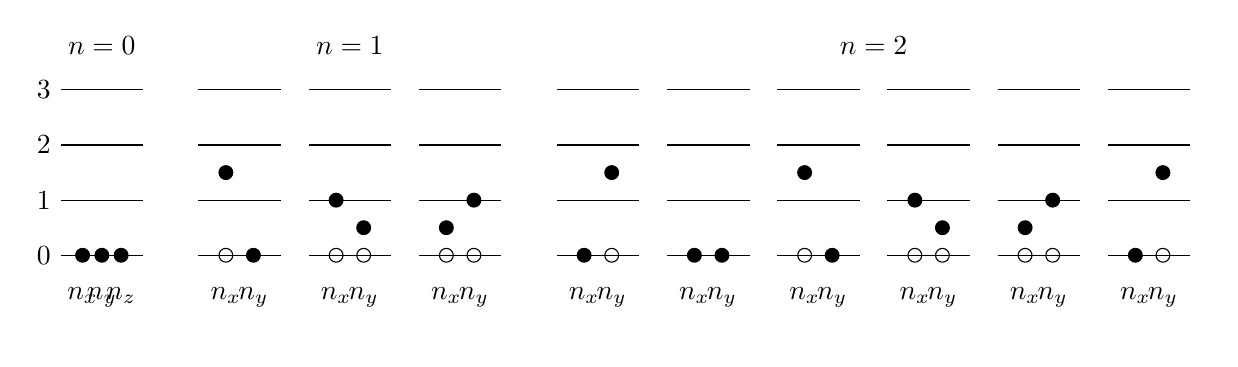
\begin{tikzpicture}[scale=0.35]
		\begin{scope}
		\foreach \i in {0,...,3}
		{
			\draw (-1,2*\i) node[anchor=east] {$\i$} --(2,2*\i);
		}
		\filldraw (-0.2,0) node[anchor=north,inner sep=.4cm] {$n_x$} circle (0.25cm); 
		\filldraw (0.5,0) node[anchor=north,inner sep=.4cm] {$n_y$} circle (0.25cm);
		\filldraw (1.2,0) node[anchor=north,inner sep=.4cm] {$n_z$} circle (0.25cm);
		\node[] at (0.5,7.6) {$n=0$};
		\end{scope}
		\begin{scope}[xshift=5cm]
		\foreach \i in {0,...,3}
		{
			\draw (-1,2*\i) --(2,2*\i);
		}
		\draw (0,0) node[anchor=north,inner sep=.4cm] {$n_x$} circle (0.25cm); 
		\filldraw (1,0) node[anchor=north,inner sep=.4cm] {$n_y$} circle (0.25cm);
		\filldraw (0,3) circle (0.25cm);
		\end{scope}
		\begin{scope}[xshift=9cm]
		\foreach \i in {0,...,3}
		{
			\draw (-1,2*\i) --(2,2*\i);
		}
		\draw (0,0) node[anchor=north,inner sep=.4cm] {$n_x$} circle (0.25cm); 
		\draw (1,0) node[anchor=north,inner sep=.4cm] {$n_y$} circle (0.25cm);
		\filldraw (0,2) circle (0.25cm); 
		\filldraw (1,1) circle (0.25cm); 
		\node[] at (0.5,7.6) {$n=1$};
		\end{scope}
		\begin{scope}[xshift=13cm]
		\foreach \i in {0,...,3}
		{
			\draw (-1,2*\i) --(2,2*\i);
		}
		\draw (0,0) node[anchor=north,inner sep=.4cm] {$n_x$} circle (0.25cm); 
		\draw (1,0) node[anchor=north,inner sep=.4cm] {$n_y$} circle (0.25cm);
		\filldraw (0,1) circle (0.25cm); 
		\filldraw (1,2) circle (0.25cm); 
		\end{scope}
		\begin{scope}[xshift=18cm]
		\foreach \i in {0,...,3}
		{
			\draw (-1,2*\i) --(2,2*\i);
		}
		\filldraw (0,0) node[anchor=north,inner sep=.4cm] {$n_x$} circle (0.25cm); 
		\draw (1,0) node[anchor=north,inner sep=.4cm] {$n_y$} circle (0.25cm);
		\filldraw (1,3) circle (0.25cm); 
		\end{scope}
		\begin{scope}[xshift=22cm]
		\foreach \i in {0,...,3}
		{
			\draw (-1,2*\i) --(2,2*\i);
		}
		\filldraw (0,0) node[anchor=north,inner sep=.4cm] {$n_x$} circle (0.25cm); 
		\filldraw (1,0) node[anchor=north,inner sep=.4cm] {$n_y$} circle (0.25cm);
		\end{scope}
		\begin{scope}[xshift=26cm]
		\foreach \i in {0,...,3}
		{
			\draw (-1,2*\i) --(2,2*\i);
		}
		\draw (0,0) node[anchor=north,inner sep=.4cm] {$n_x$} circle (0.25cm); 
		\filldraw (1,0) node[anchor=north,inner sep=.4cm] {$n_y$} circle (0.25cm);
		\filldraw (0,3) circle (0.25cm);
		\node[] at (2.5,7.6) {$n=2$};
		\end{scope}
		\begin{scope}[xshift=30cm]
		\foreach \i in {0,...,3}
		{
			\draw (-1,2*\i) --(2,2*\i);
		}
		\draw (0,0) node[anchor=north,inner sep=.4cm] {$n_x$} circle (0.25cm); 
		\draw (1,0) node[anchor=north,inner sep=.4cm] {$n_y$} circle (0.25cm);
		\filldraw (0,2) circle (0.25cm); 
		\filldraw (1,1) circle (0.25cm); 
		\end{scope}
		\begin{scope}[xshift=34cm]
		\foreach \i in {0,...,3}
		{
			\draw (-1,2*\i) --(2,2*\i);
		}
		\draw (0,0) node[anchor=north,inner sep=.4cm] {$n_x$} circle (0.25cm); 
		\draw (1,0) node[anchor=north,inner sep=.4cm] {$n_y$} circle (0.25cm);
		\filldraw (0,1) circle (0.25cm); 
		\filldraw (1,2) circle (0.25cm); 
		\end{scope}
		\begin{scope}[xshift=38cm]
		\foreach \i in {0,...,3}
		{
			\draw (-1,2*\i) --(2,2*\i);
		}
		\filldraw (0,0) node[anchor=north,inner sep=.4cm] {$n_x$} circle (0.25cm); 
		\draw (1,0) node[anchor=north,inner sep=.4cm] {$n_y$} circle (0.25cm);
		\filldraw (1,3) circle (0.25cm); 
		\end{scope}
		\end{tikzpicture}
	\end{center}

	\begin{center}
		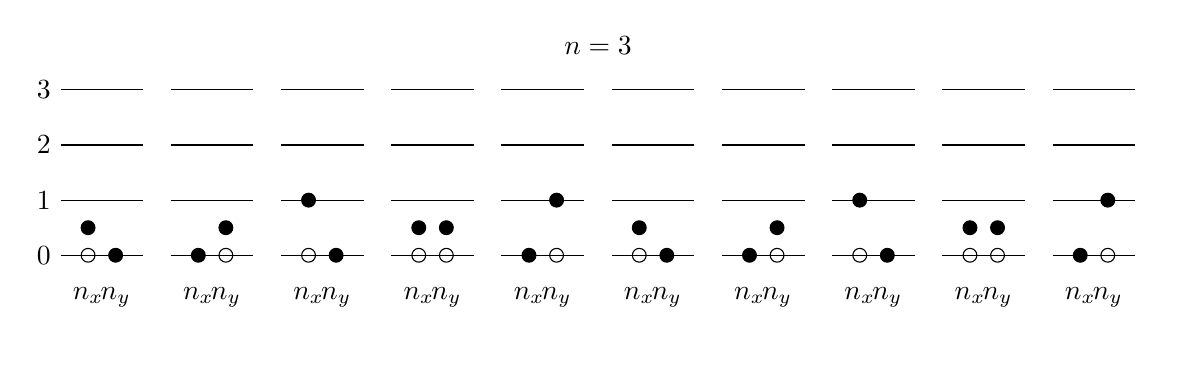
\begin{tikzpicture}[scale=0.35]
		\begin{scope}
		\foreach \i in {0,...,3}
		{
			\draw (-1,2*\i) node[anchor=east] {$\i$} --(2,2*\i);
		}
		\draw (0,0) node[anchor=north,inner sep=.4cm] {$n_x$} circle (0.25cm); 
		\filldraw (1,0) node[anchor=north,inner sep=.4cm] {$n_y$} circle (0.25cm);
		\filldraw (0,1) circle (0.25cm);
		\end{scope}
		\begin{scope}[xshift=4cm]
		\foreach \i in {0,...,3}
		{
			\draw (-1,2*\i) --(2,2*\i);
		}
		\filldraw (0,0) node[anchor=north,inner sep=.4cm] {$n_x$} circle (0.25cm); 
		\draw (1,0) node[anchor=north,inner sep=.4cm] {$n_y$} circle (0.25cm);
		\filldraw (1,1) circle (0.25cm); 
		\end{scope}
		\begin{scope}[xshift=8cm]
		\foreach \i in {0,...,3}
		{
			\draw (-1,2*\i) --(2,2*\i);
		}
		\draw (0,0) node[anchor=north,inner sep=.4cm] {$n_x$} circle (0.25cm); 
		\filldraw (1,0) node[anchor=north,inner sep=.4cm] {$n_y$} circle (0.25cm);
		\filldraw (0,2) circle (0.25cm);
		\end{scope}
		\begin{scope}[xshift=12cm]
		\foreach \i in {0,...,3}
		{
			\draw (-1,2*\i) --(2,2*\i);
		}
		\draw (0,0) node[anchor=north,inner sep=.4cm] {$n_x$} circle (0.25cm); 
		\draw (1,0) node[anchor=north,inner sep=.4cm] {$n_y$} circle (0.25cm);
		\filldraw (0,1) circle (0.25cm); 
		\filldraw (1,1) circle (0.25cm);
		\end{scope}
		\begin{scope}[xshift=16cm]
		\foreach \i in {0,...,3}
		{
			\draw (-1,2*\i) --(2,2*\i);
		}
		\filldraw (0,0) node[anchor=north,inner sep=.4cm] {$n_x$} circle (0.25cm); 
		\draw (1,0) node[anchor=north,inner sep=.4cm] {$n_y$} circle (0.25cm); 
		\filldraw (1,2) circle (0.25cm);
		\node[] at (2.5,7.6) {$n=3$};
		\end{scope}
		\begin{scope}[xshift=20cm]
		\foreach \i in {0,...,3}
		{
			\draw (-1,2*\i) --(2,2*\i);
		}
		\draw (0,0) node[anchor=north,inner sep=.4cm] {$n_x$} circle (0.25cm); 
		\filldraw (1,0) node[anchor=north,inner sep=.4cm] {$n_y$} circle (0.25cm);
		\filldraw (0,1) circle (0.25cm);
		\end{scope}
		\begin{scope}[xshift=24cm]
		\foreach \i in {0,...,3}
		{
			\draw (-1,2*\i) --(2,2*\i);
		}
		\filldraw (0,0) node[anchor=north,inner sep=.4cm] {$n_x$} circle (0.25cm); 
		\draw (1,0) node[anchor=north,inner sep=.4cm] {$n_y$} circle (0.25cm);
		\filldraw (1,1) circle (0.25cm); 
		\end{scope}
		\begin{scope}[xshift=28cm]
		\foreach \i in {0,...,3}
		{
			\draw (-1,2*\i) --(2,2*\i);
		}
		\draw (0,0) node[anchor=north,inner sep=.4cm] {$n_x$} circle (0.25cm); 
		\filldraw (1,0) node[anchor=north,inner sep=.4cm] {$n_y$} circle (0.25cm);
		\filldraw (0,2) circle (0.25cm);
		\end{scope}
		\begin{scope}[xshift=32cm]
		\foreach \i in {0,...,3}
		{
			\draw (-1,2*\i) --(2,2*\i);
		}
		\draw (0,0) node[anchor=north,inner sep=.4cm] {$n_x$} circle (0.25cm); 
		\draw (1,0) node[anchor=north,inner sep=.4cm] {$n_y$} circle (0.25cm);
		\filldraw (0,1) circle (0.25cm); 
		\filldraw (1,1) circle (0.25cm);
		\end{scope}
		\begin{scope}[xshift=36cm]
		\foreach \i in {0,...,3}
		{
			\draw (-1,2*\i) --(2,2*\i);
		}
		\filldraw (0,0) node[anchor=north,inner sep=.4cm] {$n_x$} circle (0.25cm); 
		\draw (1,0) node[anchor=north,inner sep=.4cm] {$n_y$} circle (0.25cm); 
		\filldraw (1,2) circle (0.25cm);
		\end{scope}
		\end{tikzpicture}
	\end{center}
	\caption{Possible states of a three dimensional harmonic oscillator.}
	\label{fig:schematic_3d}
\end{figure}

\section{Quantum Double Dot}
Another historically important quantum system is the double dot system, which, similarly to the quantum single dot, can be solved analytically. Unlike the single-well potential, the double-well potential is not unique, there exist multiple widely used double-well potentials, but they all usually are on the form
\begin{equation}
u_i=\frac{1}{2}\omega^2\bigg[|x_i|^n-\Big(\frac{b}{2}\Big)^n\bigg]^2
\label{eq:doublewell}
\end{equation}
in one direction with $b$ as the distance between the wells and $n$ as an arbitrary integer. \cite{jelic_double_2012} Setting $n=1$ gives two parabolic wells with a sharp local maximum at $x=0$, while $n=2$ gives a smoother but steeper well. In figure \eqref{fig:doublewell} the potential is plotted for $n=1,2$ and $3$.

\begin{figure}
	\centering
	% This file was created by matplotlib2tikz v0.7.4.
\begin{tikzpicture}

\begin{axis}[
legend cell align={left},
legend style={at={(0.5,0.91)}, anchor=north, draw=white!80.0!black},
%axis background/.style={fill=white!89.80392156862746!black},
axis line style={black},
tick align=outside,
tick pos=left,
%x grid style={black},
xlabel={$x$},
xmajorgrids,
xmin=-3.2, xmax=3.2,
xtick style={color=black},
%y grid style={black},
ylabel={$V_i^{\text{DW}}(x)$},
ymajorgrids,
ymin=0, ymax=8,
ytick style={color=black}
]
\addplot [thick, color0]
table {%
-3 8
-2.99399399399399 7.95202409616824
-2.98798798798799 7.90419248076906
-2.98198198198198 7.85650515380245
-2.97597597597598 7.80896211526842
-2.96996996996997 7.76156336516697
-2.96396396396396 7.71430890349809
-2.95795795795796 7.66719873026179
-2.95195195195195 7.62023284545807
-2.94594594594595 7.57341124908693
-2.93993993993994 7.52673394114836
-2.93393393393393 7.48020092164236
-2.92792792792793 7.43381219056895
-2.92192192192192 7.38756774792811
-2.91591591591592 7.34146759371985
-2.90990990990991 7.29551172794416
-2.9039039039039 7.24970015060105
-2.8978978978979 7.20403286169052
-2.89189189189189 7.15850986121257
-2.88588588588589 7.11313114916719
-2.87987987987988 7.06789672555438
-2.87387387387387 7.02280659037416
-2.86786786786787 6.97786074362651
-2.86186186186186 6.93305918531144
-2.85585585585586 6.88840191542894
-2.84984984984985 6.84388893397902
-2.84384384384384 6.79952024096168
-2.83783783783784 6.75529583637692
-2.83183183183183 6.71121572022473
-2.82582582582583 6.66727989250512
-2.81981981981982 6.62348835321808
-2.81381381381381 6.57984110236362
-2.80780780780781 6.53633813994174
-2.8018018018018 6.49297946595244
-2.7957957957958 6.44976508039571
-2.78978978978979 6.40669498327156
-2.78378378378378 6.36376917457999
-2.77777777777778 6.32098765432099
-2.77177177177177 6.27835042249457
-2.76576576576577 6.23585747910072
-2.75975975975976 6.19350882413946
-2.75375375375375 6.15130445761076
-2.74774774774775 6.10924437951465
-2.74174174174174 6.06732858985111
-2.73573573573574 6.02555708862015
-2.72972972972973 5.98392987582177
-2.72372372372372 5.94244695145596
-2.71771771771772 5.90110831552273
-2.71171171171171 5.85991396802207
-2.70570570570571 5.818863908954
-2.6996996996997 5.7779581383185
-2.69369369369369 5.73719665611558
-2.68768768768769 5.69657946234523
-2.68168168168168 5.65610655700746
-2.67567567567568 5.61577794010226
-2.66966966966967 5.57559361162965
-2.66366366366366 5.53555357158961
-2.65765765765766 5.49565781998214
-2.65165165165165 5.45590635680726
-2.64564564564565 5.41629918206495
-2.63963963963964 5.37683629575522
-2.63363363363363 5.33751769787806
-2.62762762762763 5.29834338843348
-2.62162162162162 5.25931336742147
-2.61561561561562 5.22042763484205
-2.60960960960961 5.1816861906952
-2.6036036036036 5.14308903498093
-2.5975975975976 5.10463616769923
-2.59159159159159 5.06632758885011
-2.58558558558559 5.02816329843357
-2.57957957957958 4.9901432964496
-2.57357357357357 4.95226758289821
-2.56756756756757 4.9145361577794
-2.56156156156156 4.87694902109316
-2.55555555555556 4.8395061728395
-2.54954954954955 4.80220761301842
-2.54354354354354 4.76505334162992
-2.53753753753754 4.72804335867399
-2.53153153153153 4.69117766415064
-2.52552552552553 4.65445625805986
-2.51951951951952 4.61787914040166
-2.51351351351351 4.58144631117604
-2.50750750750751 4.545157770383
-2.5015015015015 4.50901351802253
-2.4954954954955 4.47301355409463
-2.48948948948949 4.43715787859932
-2.48348348348348 4.40144649153658
-2.47747747747748 4.36587939290642
-2.47147147147147 4.33045658270883
-2.46546546546547 4.29517806094383
-2.45945945945946 4.2600438276114
-2.45345345345345 4.22505388271154
-2.44744744744745 4.19020822624426
-2.44144144144144 4.15550685820956
-2.43543543543544 4.12094977860743
-2.42942942942943 4.08653698743789
-2.42342342342342 4.05226848470092
-2.41741741741742 4.01814427039652
-2.41141141141141 3.9841643445247
-2.40540540540541 3.95032870708546
-2.3993993993994 3.9166373580788
-2.39339339339339 3.88309029750471
-2.38738738738739 3.8496875253632
-2.38138138138138 3.81642904165427
-2.37537537537538 3.78331484637791
-2.36936936936937 3.75034493953413
-2.36336336336336 3.71751932112293
-2.35735735735736 3.6848379911443
-2.35135135135135 3.65230094959825
-2.34534534534535 3.61990819648477
-2.33933933933934 3.58765973180388
-2.33333333333333 3.55555555555556
-2.32732732732733 3.52359566773981
-2.32132132132132 3.49178006835664
-2.31531531531532 3.46010875740605
-2.30930930930931 3.42858173488804
-2.3033033033033 3.39719900080261
-2.2972972972973 3.36596055514974
-2.29129129129129 3.33486639792946
-2.28528528528529 3.30391652914175
-2.27927927927928 3.27311094878663
-2.27327327327327 3.24244965686407
-2.26726726726727 3.2119326533741
-2.26126126126126 3.1815599383167
-2.25525525525526 3.15133151169187
-2.24924924924925 3.12124737349963
-2.24324324324324 3.09130752373995
-2.23723723723724 3.06151196241286
-2.23123123123123 3.03186068951835
-2.22522522522523 3.00235370505641
-2.21921921921922 2.97299100902705
-2.21321321321321 2.94377260143026
-2.20720720720721 2.91469848226605
-2.2012012012012 2.88576865153442
-2.1951951951952 2.85698310923536
-2.18918918918919 2.82834185536888
-2.18318318318318 2.79984488993498
-2.17717717717718 2.77149221293365
-2.17117117117117 2.74328382436491
-2.16516516516517 2.71521972422873
-2.15915915915916 2.68729991252514
-2.15315315315315 2.65952438925412
-2.14714714714715 2.63189315441568
-2.14114114114114 2.60440620800981
-2.13513513513514 2.57706355003652
-2.12912912912913 2.54986518049581
-2.12312312312312 2.52281109938767
-2.11711711711712 2.49590130671212
-2.11111111111111 2.46913580246914
-2.10510510510511 2.44251458665873
-2.0990990990991 2.4160376592809
-2.09309309309309 2.38970502033565
-2.08708708708709 2.36351666982298
-2.08108108108108 2.33747260774288
-2.07507507507508 2.31157283409536
-2.06906906906907 2.28581734888041
-2.06306306306306 2.26020615209804
-2.05705705705706 2.23473924374825
-2.05105105105105 2.20941662383104
-2.04504504504505 2.1842382923464
-2.03903903903904 2.15920424929434
-2.03303303303303 2.13431449467485
-2.02702702702703 2.10956902848795
-2.02102102102102 2.08496785073362
-2.01501501501502 2.06051096141186
-2.00900900900901 2.03619836052268
-2.003003003003 2.01203004806608
-1.996996996997 1.98800602404206
-1.99099099099099 1.96412628845061
-1.98498498498498 1.94039084129174
-1.97897897897898 1.91679968256545
-1.97297297297297 1.89335281227173
-1.96696696696697 1.87005023041059
-1.96096096096096 1.84689193698203
-1.95495495495495 1.82387793198604
-1.94894894894895 1.80100821542263
-1.94294294294294 1.7782827872918
-1.93693693693694 1.75570164759354
-1.93093093093093 1.73326479632786
-1.92492492492492 1.71097223349476
-1.91891891891892 1.68882395909423
-1.91291291291291 1.66681997312628
-1.90690690690691 1.64496027559091
-1.9009009009009 1.62324486648811
-1.89489489489489 1.60167374581789
-1.88888888888889 1.58024691358025
-1.88288288288288 1.55896436977518
-1.87687687687688 1.53782611440269
-1.87087087087087 1.51683214746278
-1.86486486486486 1.49598246895544
-1.85885885885886 1.47527707888068
-1.85285285285285 1.4547159772385
-1.84684684684685 1.43429916402889
-1.84084084084084 1.41402663925186
-1.83483483483483 1.39389840290741
-1.82882882882883 1.37391445499554
-1.82282282282282 1.35407479551624
-1.81681681681682 1.33437942446951
-1.81081081081081 1.31482834185537
-1.8048048048048 1.2954215476738
-1.7987987987988 1.27615904192481
-1.79279279279279 1.25704082460839
-1.78678678678679 1.23806689572455
-1.78078078078078 1.21923725527329
-1.77477477477477 1.20055190325461
-1.76876876876877 1.1820108396685
-1.76276276276276 1.16361406451497
-1.75675675675676 1.14536157779401
-1.75075075075075 1.12725337950563
-1.74474474474474 1.10928946964983
-1.73873873873874 1.0914698482266
-1.73273273273273 1.07379451523596
-1.72672672672673 1.05626347067789
-1.72072072072072 1.03887671455239
-1.71471471471471 1.02163424685947
-1.70870870870871 1.00453606759913
-1.7027027027027 0.987582176771366
-1.6966966966967 0.970772574376178
-1.69069069069069 0.954107260413567
-1.68468468468468 0.937586234883532
-1.67867867867868 0.921209497786074
-1.67267267267267 0.904977049121193
-1.66666666666667 0.888888888888889
-1.66066066066066 0.872945017089161
-1.65465465465465 0.857145433722011
-1.64864864864865 0.841490138787436
-1.64264264264264 0.825979132285439
-1.63663663663664 0.810612414216018
-1.63063063063063 0.795389984579174
-1.62462462462462 0.780311843374906
-1.61861861861862 0.765377990603216
-1.61261261261261 0.750588426264102
-1.60660660660661 0.735943150357565
-1.6006006006006 0.721442162883604
-1.59459459459459 0.70708546384222
-1.58858858858859 0.692873053233414
-1.58258258258258 0.678804931057183
-1.57657657657658 0.66488109731353
-1.57057057057057 0.651101552002453
-1.56456456456456 0.637466295123953
-1.55855855855856 0.62397532667803
-1.55255255255255 0.610628646664683
-1.54654654654655 0.597426255083913
-1.54054054054054 0.58436815193572
-1.53453453453453 0.571454337220103
-1.52852852852853 0.558684810937063
-1.52252252252252 0.5460595730866
-1.51651651651652 0.533578623668714
-1.51051051051051 0.521241962683404
-1.5045045045045 0.509049590130671
-1.4984984984985 0.497001506010515
-1.49249249249249 0.485097710322936
-1.48648648648649 0.473338203067933
-1.48048048048048 0.461722984245507
-1.47447447447447 0.450252053855657
-1.46846846846847 0.438925411898385
-1.46246246246246 0.427743058373689
-1.45645645645646 0.41670499328157
-1.45045045045045 0.405811216622028
-1.44444444444444 0.395061728395062
-1.43843843843844 0.384456528600673
-1.43243243243243 0.373995617238861
-1.42642642642643 0.363678994309625
-1.42042042042042 0.353506659812966
-1.41441441441441 0.343478613748884
-1.40840840840841 0.333594856117379
-1.4024024024024 0.32385538691845
-1.3963963963964 0.314260206152098
-1.39039039039039 0.304809313818323
-1.38438438438438 0.295502709917124
-1.37837837837838 0.286340394448502
-1.37237237237237 0.277322367412458
-1.36636636636637 0.268448628808989
-1.36036036036036 0.259719178638098
-1.35435435435435 0.251134016899783
-1.34834834834835 0.242693143594044
-1.34234234234234 0.234396558720883
-1.33633633633634 0.226244262280298
-1.33033033033033 0.21823625427229
-1.32432432432432 0.210372534696859
-1.31831831831832 0.202653103554004
-1.31231231231231 0.195077960843727
-1.30630630630631 0.187647106566025
-1.3003003003003 0.180360540720901
-1.29429429429429 0.173218263308353
-1.28828828828829 0.166220274328382
-1.28228228228228 0.159366573780988
-1.27627627627628 0.152657161666171
-1.27027027027027 0.14609203798393
-1.26426426426426 0.139671202734266
-1.25825825825826 0.133394655917178
-1.25225225225225 0.127262397532668
-1.24624624624625 0.121274427580734
-1.24024024024024 0.115430746061377
-1.23423423423423 0.109731352974596
-1.22822822822823 0.104176248320392
-1.22222222222222 0.0987654320987655
-1.21621621621622 0.0934989043097151
-1.21021021021021 0.0883766649532415
-1.2042042042042 0.0833987140293447
-1.1981981981982 0.0785650515380245
-1.19219219219219 0.0738756774792812
-1.18618618618619 0.0693305918531144
-1.18018018018018 0.0649297946595243
-1.17417417417417 0.0606732858985112
-1.16816816816817 0.0565610655700746
-1.16216216216216 0.0525931336742148
-1.15615615615616 0.0487694902109317
-1.15015015015015 0.0450901351802252
-1.14414414414414 0.0415550685820957
-1.13813813813814 0.0381642904165427
-1.13213213213213 0.0349178006835664
-1.12612612612613 0.031815599383167
-1.12012012012012 0.0288576865153442
-1.11411411411411 0.0260440620800982
-1.10810810810811 0.0233747260774288
-1.1021021021021 0.0208496785073361
-1.0960960960961 0.0184689193698203
-1.09009009009009 0.0162324486648811
-1.08408408408408 0.0141402663925187
-1.07807807807808 0.0121923725527329
-1.07207207207207 0.0103887671455239
-1.06606606606607 0.00872945017089163
-1.06006006006006 0.00721442162883604
-1.05405405405405 0.00584368151935722
-1.04804804804805 0.00461722984245507
-1.04204204204204 0.00353506659812965
-1.03603603603604 0.00259719178638099
-1.03003003003003 0.00180360540720901
-1.02402402402402 0.00115430746061378
-1.01801801801802 0.000649297946595247
-1.01201201201201 0.000288576865153439
-1.00600600600601 7.21442162883625e-05
-1 0
-0.993993993993994 7.21442162883625e-05
-0.987987987987988 0.00028857686515345
-0.981981981981982 0.000649297946595231
-0.975975975975976 0.00115430746061376
-0.96996996996997 0.00180360540720901
-0.963963963963964 0.00259719178638099
-0.957957957957958 0.00353506659812969
-0.951951951951952 0.00461722984245503
-0.945945945945946 0.00584368151935717
-0.93993993993994 0.00721442162883604
-0.933933933933934 0.00872945017089163
-0.927927927927928 0.0103887671455239
-0.921921921921922 0.0121923725527328
-0.915915915915916 0.0141402663925186
-0.90990990990991 0.0162324486648811
-0.903903903903904 0.0184689193698203
-0.897897897897898 0.0208496785073362
-0.891891891891892 0.0233747260774287
-0.885885885885886 0.0260440620800981
-0.87987987987988 0.0288576865153442
-0.873873873873874 0.031815599383167
-0.867867867867868 0.0349178006835665
-0.861861861861862 0.0381642904165425
-0.855855855855856 0.0415550685820955
-0.84984984984985 0.0450901351802252
-0.843843843843844 0.0487694902109317
-0.837837837837838 0.0525931336742148
-0.831831831831832 0.0565610655700744
-0.825825825825826 0.060673285898511
-0.81981981981982 0.0649297946595243
-0.813813813813814 0.0693305918531144
-0.807807807807808 0.0738756774792812
-0.801801801801802 0.0785650515380247
-0.795795795795796 0.0833987140293445
-0.78978978978979 0.0883766649532415
-0.783783783783784 0.0934989043097151
-0.777777777777778 0.0987654320987655
-0.771771771771772 0.104176248320393
-0.765765765765766 0.109731352974596
-0.75975975975976 0.115430746061377
-0.753753753753754 0.121274427580734
-0.747747747747748 0.127262397532668
-0.741741741741742 0.133394655917179
-0.735735735735736 0.139671202734266
-0.72972972972973 0.14609203798393
-0.723723723723724 0.152657161666171
-0.717717717717718 0.159366573780988
-0.711711711711712 0.166220274328383
-0.705705705705706 0.173218263308353
-0.6996996996997 0.180360540720901
-0.693693693693694 0.187647106566025
-0.687687687687688 0.195077960843727
-0.681681681681682 0.202653103554005
-0.675675675675676 0.210372534696859
-0.66966966966967 0.21823625427229
-0.663663663663664 0.226244262280298
-0.657657657657658 0.234396558720883
-0.651651651651652 0.242693143594045
-0.645645645645646 0.251134016899782
-0.63963963963964 0.259719178638097
-0.633633633633634 0.268448628808989
-0.627627627627628 0.277322367412458
-0.621621621621621 0.286340394448503
-0.615615615615616 0.295502709917124
-0.60960960960961 0.304809313818323
-0.603603603603604 0.314260206152098
-0.597597597597598 0.32385538691845
-0.591591591591591 0.333594856117379
-0.585585585585586 0.343478613748884
-0.57957957957958 0.353506659812966
-0.573573573573574 0.363678994309625
-0.567567567567568 0.373995617238861
-0.561561561561561 0.384456528600673
-0.555555555555555 0.395061728395062
-0.54954954954955 0.405811216622027
-0.543543543543544 0.41670499328157
-0.537537537537538 0.427743058373689
-0.531531531531531 0.438925411898385
-0.525525525525525 0.450252053855658
-0.51951951951952 0.461722984245506
-0.513513513513514 0.473338203067933
-0.507507507507508 0.485097710322936
-0.501501501501501 0.497001506010515
-0.495495495495495 0.509049590130672
-0.48948948948949 0.521241962683404
-0.483483483483484 0.533578623668714
-0.477477477477477 0.5460595730866
-0.471471471471471 0.558684810937063
-0.465465465465465 0.571454337220103
-0.45945945945946 0.584368151935719
-0.453453453453454 0.597426255083913
-0.447447447447447 0.610628646664683
-0.441441441441441 0.62397532667803
-0.435435435435435 0.637466295123953
-0.42942942942943 0.651101552002452
-0.423423423423424 0.66488109731353
-0.417417417417417 0.678804931057183
-0.411411411411411 0.692873053233414
-0.405405405405405 0.707085463842221
-0.3993993993994 0.721442162883604
-0.393393393393394 0.735943150357564
-0.387387387387387 0.750588426264102
-0.381381381381381 0.765377990603216
-0.375375375375375 0.780311843374907
-0.36936936936937 0.795389984579173
-0.363363363363364 0.810612414216017
-0.357357357357357 0.825979132285439
-0.351351351351351 0.841490138787436
-0.345345345345345 0.857145433722011
-0.33933933933934 0.872945017089161
-0.333333333333333 0.888888888888889
-0.327327327327327 0.904977049121193
-0.321321321321321 0.921209497786074
-0.315315315315315 0.937586234883532
-0.30930930930931 0.954107260413566
-0.303303303303303 0.970772574376178
-0.297297297297297 0.987582176771366
-0.291291291291291 1.00453606759913
-0.285285285285285 1.02163424685947
-0.279279279279279 1.03887671455239
-0.273273273273273 1.05626347067788
-0.267267267267267 1.07379451523596
-0.261261261261261 1.0914698482266
-0.255255255255255 1.10928946964983
-0.249249249249249 1.12725337950563
-0.243243243243243 1.14536157779401
-0.237237237237237 1.16361406451497
-0.231231231231231 1.1820108396685
-0.225225225225225 1.20055190325461
-0.219219219219219 1.21923725527329
-0.213213213213213 1.23806689572455
-0.207207207207207 1.25704082460839
-0.201201201201201 1.27615904192481
-0.195195195195195 1.2954215476738
-0.189189189189189 1.31482834185537
-0.183183183183183 1.33437942446951
-0.177177177177177 1.35407479551624
-0.171171171171171 1.37391445499554
-0.165165165165165 1.39389840290741
-0.159159159159159 1.41402663925187
-0.153153153153153 1.43429916402889
-0.147147147147147 1.4547159772385
-0.141141141141141 1.47527707888068
-0.135135135135135 1.49598246895544
-0.129129129129129 1.51683214746278
-0.123123123123123 1.53782611440269
-0.117117117117117 1.55896436977518
-0.111111111111111 1.58024691358025
-0.105105105105105 1.60167374581789
-0.099099099099099 1.62324486648811
-0.0930930930930933 1.64496027559091
-0.0870870870870872 1.66681997312628
-0.0810810810810811 1.68882395909423
-0.075075075075075 1.71097223349476
-0.069069069069069 1.73326479632786
-0.0630630630630633 1.75570164759354
-0.0570570570570572 1.7782827872918
-0.0510510510510511 1.80100821542263
-0.045045045045045 1.82387793198604
-0.0390390390390389 1.84689193698203
-0.0330330330330328 1.87005023041059
-0.0270270270270272 1.89335281227173
-0.0210210210210211 1.91679968256545
-0.015015015015015 1.94039084129174
-0.00900900900900892 1.96412628845061
-0.00300300300300282 1.98800602404206
0.00300300300300282 1.98800602404206
0.00900900900900892 1.96412628845061
0.015015015015015 1.94039084129174
0.0210210210210211 1.91679968256545
0.0270270270270272 1.89335281227173
0.0330330330330328 1.87005023041059
0.0390390390390389 1.84689193698203
0.045045045045045 1.82387793198604
0.0510510510510511 1.80100821542263
0.0570570570570572 1.7782827872918
0.0630630630630629 1.75570164759354
0.069069069069069 1.73326479632786
0.075075075075075 1.71097223349476
0.0810810810810811 1.68882395909423
0.0870870870870872 1.66681997312628
0.0930930930930929 1.64496027559091
0.099099099099099 1.62324486648811
0.105105105105105 1.60167374581789
0.111111111111111 1.58024691358025
0.117117117117117 1.55896436977518
0.123123123123123 1.53782611440269
0.129129129129129 1.51683214746278
0.135135135135135 1.49598246895544
0.141141141141141 1.47527707888068
0.147147147147147 1.4547159772385
0.153153153153153 1.43429916402889
0.159159159159159 1.41402663925187
0.165165165165165 1.39389840290741
0.171171171171171 1.37391445499554
0.177177177177177 1.35407479551624
0.183183183183183 1.33437942446952
0.189189189189189 1.31482834185537
0.195195195195195 1.2954215476738
0.201201201201201 1.27615904192481
0.207207207207207 1.25704082460839
0.213213213213213 1.23806689572455
0.219219219219219 1.21923725527329
0.225225225225225 1.20055190325461
0.231231231231231 1.1820108396685
0.237237237237237 1.16361406451497
0.243243243243243 1.14536157779401
0.249249249249249 1.12725337950563
0.255255255255255 1.10928946964983
0.261261261261261 1.0914698482266
0.267267267267267 1.07379451523596
0.273273273273273 1.05626347067788
0.279279279279279 1.03887671455239
0.285285285285285 1.02163424685947
0.291291291291291 1.00453606759913
0.297297297297297 0.987582176771366
0.303303303303303 0.970772574376178
0.309309309309309 0.954107260413567
0.315315315315315 0.937586234883532
0.321321321321321 0.921209497786074
0.327327327327327 0.904977049121193
0.333333333333333 0.888888888888889
0.339339339339339 0.872945017089162
0.345345345345345 0.857145433722011
0.351351351351351 0.841490138787436
0.357357357357357 0.825979132285439
0.363363363363364 0.810612414216017
0.369369369369369 0.795389984579174
0.375375375375375 0.780311843374907
0.381381381381381 0.765377990603216
0.387387387387387 0.750588426264102
0.393393393393394 0.735943150357564
0.399399399399399 0.721442162883605
0.405405405405405 0.707085463842221
0.411411411411411 0.692873053233414
0.417417417417417 0.678804931057183
0.423423423423424 0.66488109731353
0.429429429429429 0.651101552002453
0.435435435435435 0.637466295123953
0.441441441441441 0.62397532667803
0.447447447447447 0.610628646664683
0.453453453453454 0.597426255083913
0.45945945945946 0.584368151935719
0.465465465465465 0.571454337220103
0.471471471471471 0.558684810937063
0.477477477477477 0.5460595730866
0.483483483483484 0.533578623668714
0.48948948948949 0.521241962683404
0.495495495495495 0.509049590130672
0.501501501501501 0.497001506010515
0.507507507507508 0.485097710322936
0.513513513513514 0.473338203067933
0.51951951951952 0.461722984245506
0.525525525525525 0.450252053855658
0.531531531531531 0.438925411898385
0.537537537537538 0.427743058373689
0.543543543543544 0.41670499328157
0.54954954954955 0.405811216622027
0.555555555555555 0.395061728395062
0.561561561561561 0.384456528600673
0.567567567567568 0.373995617238861
0.573573573573574 0.363678994309625
0.57957957957958 0.353506659812966
0.585585585585585 0.343478613748884
0.591591591591591 0.333594856117379
0.597597597597598 0.32385538691845
0.603603603603604 0.314260206152098
0.60960960960961 0.304809313818323
0.615615615615615 0.295502709917125
0.621621621621621 0.286340394448503
0.627627627627628 0.277322367412458
0.633633633633634 0.268448628808989
0.63963963963964 0.259719178638097
0.645645645645645 0.251134016899783
0.651651651651652 0.242693143594045
0.657657657657658 0.234396558720883
0.663663663663664 0.226244262280298
0.66966966966967 0.21823625427229
0.675675675675675 0.210372534696859
0.681681681681682 0.202653103554005
0.687687687687688 0.195077960843727
0.693693693693694 0.187647106566025
0.6996996996997 0.180360540720901
0.705705705705705 0.173218263308354
0.711711711711712 0.166220274328383
0.717717717717718 0.159366573780988
0.723723723723724 0.152657161666171
0.72972972972973 0.14609203798393
0.735735735735736 0.139671202734266
0.741741741741742 0.133394655917179
0.747747747747748 0.127262397532668
0.753753753753754 0.121274427580734
0.75975975975976 0.115430746061377
0.765765765765766 0.109731352974596
0.771771771771772 0.104176248320393
0.777777777777778 0.0987654320987655
0.783783783783784 0.0934989043097151
0.78978978978979 0.0883766649532415
0.795795795795796 0.0833987140293445
0.801801801801802 0.0785650515380247
0.807807807807808 0.0738756774792812
0.813813813813814 0.0693305918531144
0.81981981981982 0.0649297946595243
0.825825825825826 0.060673285898511
0.831831831831832 0.0565610655700747
0.837837837837838 0.0525931336742148
0.843843843843844 0.0487694902109317
0.84984984984985 0.0450901351802252
0.855855855855856 0.0415550685820955
0.861861861861862 0.0381642904165428
0.867867867867868 0.0349178006835665
0.873873873873874 0.031815599383167
0.87987987987988 0.0288576865153442
0.885885885885886 0.0260440620800981
0.891891891891892 0.0233747260774289
0.897897897897898 0.0208496785073362
0.903903903903904 0.0184689193698203
0.90990990990991 0.0162324486648811
0.915915915915916 0.0141402663925186
0.921921921921922 0.012192372552733
0.927927927927928 0.0103887671455239
0.933933933933934 0.00872945017089163
0.93993993993994 0.00721442162883604
0.945945945945946 0.00584368151935717
0.951951951951952 0.00461722984245512
0.957957957957958 0.00353506659812969
0.963963963963964 0.00259719178638099
0.96996996996997 0.00180360540720901
0.975975975975976 0.00115430746061376
0.981981981981982 0.000649297946595231
0.987987987987988 0.00028857686515345
0.993993993993994 7.21442162883625e-05
1 0
1.00600600600601 7.21442162883518e-05
1.01201201201201 0.00028857686515345
1.01801801801802 0.000649297946595231
1.02402402402402 0.0011543074606138
1.03003003003003 0.00180360540720901
1.03603603603604 0.00259719178638092
1.04204204204204 0.00353506659812969
1.04804804804805 0.00461722984245503
1.05405405405405 0.00584368151935727
1.06006006006006 0.00721442162883604
1.06606606606607 0.00872945017089151
1.07207207207207 0.0103887671455239
1.07807807807808 0.0121923725527328
1.08408408408408 0.0141402663925188
1.09009009009009 0.0162324486648811
1.0960960960961 0.0184689193698201
1.1021021021021 0.0208496785073362
1.10810810810811 0.0233747260774287
1.11411411411411 0.0260440620800983
1.12012012012012 0.0288576865153442
1.12612612612613 0.0318155993831667
1.13213213213213 0.0349178006835665
1.13813813813814 0.0381642904165425
1.14414414414414 0.0415550685820958
1.15015015015015 0.0450901351802252
1.15615615615616 0.0487694902109314
1.16216216216216 0.0525931336742148
1.16816816816817 0.0565610655700744
1.17417417417417 0.0606732858985113
1.18018018018018 0.0649297946595243
1.18618618618619 0.0693305918531141
1.19219219219219 0.0738756774792812
1.1981981981982 0.0785650515380243
1.2042042042042 0.0833987140293449
1.21021021021021 0.0883766649532415
1.21621621621622 0.0934989043097147
1.22222222222222 0.0987654320987655
1.22822822822823 0.104176248320392
1.23423423423423 0.109731352974596
1.24024024024024 0.115430746061377
1.24624624624625 0.121274427580733
1.25225225225225 0.127262397532668
1.25825825825826 0.133394655917178
1.26426426426426 0.139671202734266
1.27027027027027 0.14609203798393
1.27627627627628 0.15265716166617
1.28228228228228 0.159366573780988
1.28828828828829 0.166220274328382
1.29429429429429 0.173218263308354
1.3003003003003 0.180360540720901
1.30630630630631 0.187647106566025
1.31231231231231 0.195077960843727
1.31831831831832 0.202653103554004
1.32432432432432 0.210372534696859
1.33033033033033 0.21823625427229
1.33633633633634 0.226244262280298
1.34234234234234 0.234396558720883
1.34834834834835 0.242693143594044
1.35435435435435 0.251134016899783
1.36036036036036 0.259719178638097
1.36636636636637 0.26844862880899
1.37237237237237 0.277322367412458
1.37837837837838 0.286340394448502
1.38438438438438 0.295502709917125
1.39039039039039 0.304809313818323
1.3963963963964 0.314260206152099
1.4024024024024 0.32385538691845
1.40840840840841 0.333594856117378
1.41441441441441 0.343478613748884
1.42042042042042 0.353506659812966
1.42642642642643 0.363678994309626
1.43243243243243 0.373995617238861
1.43843843843844 0.384456528600672
1.44444444444444 0.395061728395062
1.45045045045045 0.405811216622027
1.45645645645646 0.416704993281571
1.46246246246246 0.427743058373689
1.46846846846847 0.438925411898384
1.47447447447447 0.450252053855658
1.48048048048048 0.461722984245506
1.48648648648649 0.473338203067934
1.49249249249249 0.485097710322936
1.4984984984985 0.497001506010514
1.5045045045045 0.509049590130672
1.51051051051051 0.521241962683404
1.51651651651652 0.533578623668714
1.52252252252252 0.5460595730866
1.52852852852853 0.558684810937062
1.53453453453453 0.571454337220103
1.54054054054054 0.584368151935719
1.54654654654655 0.597426255083913
1.55255255255255 0.610628646664683
1.55855855855856 0.623975326678029
1.56456456456456 0.637466295123953
1.57057057057057 0.651101552002452
1.57657657657658 0.664881097313531
1.58258258258258 0.678804931057183
1.58858858858859 0.692873053233413
1.59459459459459 0.707085463842221
1.6006006006006 0.721442162883604
1.60660660660661 0.735943150357566
1.61261261261261 0.750588426264102
1.61861861861862 0.765377990603215
1.62462462462462 0.780311843374907
1.63063063063063 0.795389984579173
1.63663663663664 0.810612414216019
1.64264264264264 0.825979132285439
1.64864864864865 0.841490138787435
1.65465465465465 0.857145433722011
1.66066066066066 0.872945017089161
1.66666666666667 0.88888888888889
1.67267267267267 0.904977049121193
1.67867867867868 0.921209497786073
1.68468468468468 0.937586234883532
1.69069069069069 0.954107260413566
1.6966966966967 0.970772574376179
1.7027027027027 0.987582176771366
1.70870870870871 1.00453606759913
1.71471471471471 1.02163424685947
1.72072072072072 1.03887671455239
1.72672672672673 1.05626347067789
1.73273273273273 1.07379451523596
1.73873873873874 1.0914698482266
1.74474474474474 1.10928946964983
1.75075075075075 1.12725337950563
1.75675675675676 1.14536157779401
1.76276276276276 1.16361406451497
1.76876876876877 1.1820108396685
1.77477477477477 1.20055190325461
1.78078078078078 1.21923725527329
1.78678678678679 1.23806689572455
1.79279279279279 1.25704082460839
1.7987987987988 1.27615904192481
1.8048048048048 1.2954215476738
1.81081081081081 1.31482834185537
1.81681681681682 1.33437942446952
1.82282282282282 1.35407479551624
1.82882882882883 1.37391445499553
1.83483483483483 1.39389840290741
1.84084084084084 1.41402663925186
1.84684684684685 1.43429916402889
1.85285285285285 1.4547159772385
1.85885885885886 1.47527707888068
1.86486486486486 1.49598246895544
1.87087087087087 1.51683214746278
1.87687687687688 1.53782611440269
1.88288288288288 1.55896436977518
1.88888888888889 1.58024691358025
1.89489489489489 1.60167374581789
1.9009009009009 1.62324486648811
1.90690690690691 1.64496027559091
1.91291291291291 1.66681997312628
1.91891891891892 1.68882395909423
1.92492492492492 1.71097223349476
1.93093093093093 1.73326479632786
1.93693693693694 1.75570164759354
1.94294294294294 1.7782827872918
1.94894894894895 1.80100821542263
1.95495495495495 1.82387793198604
1.96096096096096 1.84689193698203
1.96696696696697 1.87005023041059
1.97297297297297 1.89335281227173
1.97897897897898 1.91679968256545
1.98498498498498 1.94039084129174
1.99099099099099 1.96412628845061
1.996996996997 1.98800602404206
2.003003003003 2.01203004806608
2.00900900900901 2.03619836052269
2.01501501501502 2.06051096141186
2.02102102102102 2.08496785073361
2.02702702702703 2.10956902848795
2.03303303303303 2.13431449467485
2.03903903903904 2.15920424929434
2.04504504504505 2.1842382923464
2.05105105105105 2.20941662383104
2.05705705705706 2.23473924374825
2.06306306306306 2.26020615209804
2.06906906906907 2.28581734888041
2.07507507507508 2.31157283409536
2.08108108108108 2.33747260774288
2.08708708708709 2.36351666982298
2.09309309309309 2.38970502033565
2.0990990990991 2.4160376592809
2.10510510510511 2.44251458665873
2.11111111111111 2.46913580246913
2.11711711711712 2.49590130671212
2.12312312312312 2.52281109938767
2.12912912912913 2.54986518049581
2.13513513513514 2.57706355003652
2.14114114114114 2.60440620800981
2.14714714714715 2.63189315441568
2.15315315315315 2.65952438925412
2.15915915915916 2.68729991252514
2.16516516516517 2.71521972422873
2.17117117117117 2.7432838243649
2.17717717717718 2.77149221293365
2.18318318318318 2.79984488993498
2.18918918918919 2.82834185536888
2.1951951951952 2.85698310923536
2.2012012012012 2.88576865153442
2.20720720720721 2.91469848226605
2.21321321321321 2.94377260143026
2.21921921921922 2.97299100902705
2.22522522522523 3.00235370505641
2.23123123123123 3.03186068951835
2.23723723723724 3.06151196241286
2.24324324324324 3.09130752373995
2.24924924924925 3.12124737349963
2.25525525525526 3.15133151169187
2.26126126126126 3.18155993831669
2.26726726726727 3.2119326533741
2.27327327327327 3.24244965686407
2.27927927927928 3.27311094878663
2.28528528528529 3.30391652914175
2.29129129129129 3.33486639792946
2.2972972972973 3.36596055514974
2.3033033033033 3.3971990008026
2.30930930930931 3.42858173488804
2.31531531531532 3.46010875740605
2.32132132132132 3.49178006835664
2.32732732732733 3.52359566773981
2.33333333333333 3.55555555555555
2.33933933933934 3.58765973180388
2.34534534534535 3.61990819648477
2.35135135135135 3.65230094959824
2.35735735735736 3.6848379911443
2.36336336336336 3.71751932112292
2.36936936936937 3.75034493953413
2.37537537537538 3.78331484637791
2.38138138138138 3.81642904165426
2.38738738738739 3.8496875253632
2.39339339339339 3.88309029750471
2.3993993993994 3.9166373580788
2.40540540540541 3.95032870708546
2.41141141141141 3.98416434452471
2.41741741741742 4.01814427039652
2.42342342342342 4.05226848470092
2.42942942942943 4.08653698743789
2.43543543543544 4.12094977860743
2.44144144144144 4.15550685820956
2.44744744744745 4.19020822624426
2.45345345345345 4.22505388271154
2.45945945945946 4.2600438276114
2.46546546546547 4.29517806094383
2.47147147147147 4.33045658270884
2.47747747747748 4.36587939290642
2.48348348348348 4.40144649153658
2.48948948948949 4.43715787859932
2.4954954954955 4.47301355409463
2.5015015015015 4.50901351802253
2.50750750750751 4.545157770383
2.51351351351351 4.58144631117604
2.51951951951952 4.61787914040166
2.52552552552553 4.65445625805986
2.53153153153153 4.69117766415064
2.53753753753754 4.72804335867399
2.54354354354354 4.76505334162992
2.54954954954955 4.80220761301842
2.55555555555556 4.8395061728395
2.56156156156156 4.87694902109317
2.56756756756757 4.9145361577794
2.57357357357357 4.95226758289821
2.57957957957958 4.9901432964496
2.58558558558559 5.02816329843357
2.59159159159159 5.06632758885011
2.5975975975976 5.10463616769923
2.6036036036036 5.14308903498092
2.60960960960961 5.1816861906952
2.61561561561562 5.22042763484205
2.62162162162162 5.25931336742148
2.62762762762763 5.29834338843348
2.63363363363363 5.33751769787806
2.63963963963964 5.37683629575522
2.64564564564565 5.41629918206495
2.65165165165165 5.45590635680726
2.65765765765766 5.49565781998214
2.66366366366366 5.53555357158961
2.66966966966967 5.57559361162965
2.67567567567568 5.61577794010226
2.68168168168168 5.65610655700746
2.68768768768769 5.69657946234523
2.69369369369369 5.73719665611557
2.6996996996997 5.7779581383185
2.70570570570571 5.818863908954
2.71171171171171 5.85991396802208
2.71771771771772 5.90110831552273
2.72372372372372 5.94244695145596
2.72972972972973 5.98392987582177
2.73573573573574 6.02555708862015
2.74174174174174 6.06732858985111
2.74774774774775 6.10924437951465
2.75375375375375 6.15130445761076
2.75975975975976 6.19350882413946
2.76576576576577 6.23585747910072
2.77177177177177 6.27835042249457
2.77777777777778 6.32098765432099
2.78378378378378 6.36376917457998
2.78978978978979 6.40669498327156
2.7957957957958 6.44976508039571
2.8018018018018 6.49297946595244
2.80780780780781 6.53633813994174
2.81381381381381 6.57984110236362
2.81981981981982 6.62348835321808
2.82582582582583 6.66727989250512
2.83183183183183 6.71121572022473
2.83783783783784 6.75529583637692
2.84384384384384 6.79952024096168
2.84984984984985 6.84388893397902
2.85585585585586 6.88840191542894
2.86186186186186 6.93305918531144
2.86786786786787 6.97786074362651
2.87387387387387 7.02280659037415
2.87987987987988 7.06789672555438
2.88588588588589 7.11313114916718
2.89189189189189 7.15850986121257
2.8978978978979 7.20403286169052
2.9039039039039 7.24970015060105
2.90990990990991 7.29551172794416
2.91591591591592 7.34146759371984
2.92192192192192 7.38756774792811
2.92792792792793 7.43381219056895
2.93393393393393 7.48020092164237
2.93993993993994 7.52673394114836
2.94594594594595 7.57341124908692
2.95195195195195 7.62023284545807
2.95795795795796 7.66719873026179
2.96396396396396 7.7143089034981
2.96996996996997 7.76156336516697
2.97597597597598 7.80896211526842
2.98198198198198 7.85650515380245
2.98798798798799 7.90419248076906
2.99399399399399 7.95202409616824
3 8
};
\addlegendentry{$a=1$}
\addplot [thick, color1]
table {%
-3 64
-2.99399399399399 63.4252965745565
-2.98798798798799 62.8543290678273
-2.98198198198198 62.2870819279061
-2.97597597597598 61.7235396341151
-2.96996996996997 61.1636866970054
-2.96396396396396 60.6075076583569
-2.95795795795796 60.054987091178
-2.95195195195195 59.5061095997062
-2.94594594594595 58.9608598194072
-2.93993993993994 58.4192224169759
-2.93393393393393 57.8811820903356
-2.92792792792793 57.3467235686387
-2.92192192192192 56.8158316122659
-2.91591591591592 56.2884910128269
-2.90990990990991 55.7646865931601
-2.9039039039039 55.2444032073325
-2.8978978978979 54.7276257406399
-2.89189189189189 54.2143391096069
-2.88588588588589 53.7045282619868
-2.87987987987988 53.1981781767615
-2.87387387387387 52.6952738641418
-2.86786786786787 52.1958003655671
-2.86186186186186 51.6997427537056
-2.85585585585586 51.2070861324542
-2.84984984984985 50.7178156369385
-2.84384384384384 50.2319164335129
-2.83783783783784 49.7493737197605
-2.83183183183183 49.2701727244931
-2.82582582582583 48.7942987077512
-2.81981981981982 48.3217369608041
-2.81381381381381 47.8524728061498
-2.80780780780781 47.386491597515
-2.8018018018018 46.9237787198553
-2.7957957957958 46.4643195893547
-2.78978978978979 46.0080996534262
-2.78378378378378 45.5551043907114
-2.77777777777778 45.1053193110806
-2.77177177177177 44.658729955633
-2.76576576576577 44.2153218966965
-2.75975975975976 43.7750807378274
-2.75375375375375 43.3379921138112
-2.74774774774775 42.9040416906618
-2.74174174174174 42.4732151656219
-2.73573573573574 42.045498267163
-2.72972972972973 41.6208767549853
-2.72372372372372 41.1993364200177
-2.71771771771772 40.7808630844178
-2.71171171171171 40.3654426015721
-2.70570570570571 39.9530608560955
-2.6996996996997 39.543703763832
-2.69369369369369 39.1373572718541
-2.68768768768769 38.734007358463
-2.68168168168168 38.3336400331888
-2.67567567567568 37.9362413367901
-2.66966966966967 37.5417973412546
-2.66366366366366 37.1502941497983
-2.65765765765766 36.7617178968662
-2.65165165165165 36.3760547481319
-2.64564564564565 35.9932909004977
-2.63963963963964 35.6134125820949
-2.63363363363363 35.2364060522832
-2.62762762762763 34.8622576016512
-2.62162162162162 34.4909535520161
-2.61561561561562 34.1224802564239
-2.60960960960961 33.7568240991496
-2.6036036036036 33.3939714956963
-2.5975975975976 33.0339088927964
-2.59159159159159 32.6766227684108
-2.58558558558559 32.3220996317292
-2.57957957957958 31.9703260231699
-2.57357357357357 31.62128851438
-2.56756756756757 31.2749737082353
-2.56156156156156 30.9313682388405
-2.55555555555556 30.5904587715287
-2.54954954954955 30.2522320028621
-2.54354354354354 29.9166746606314
-2.53753753753754 29.5837735038559
-2.53153153153153 29.253515322784
-2.52552552552553 28.9258869388926
-2.51951951951952 28.6008752048872
-2.51351351351351 28.2784670047024
-2.50750750750751 27.9586492535011
-2.5015015015015 27.6414088976753
-2.4954954954955 27.3267329148455
-2.48948948948949 27.014608313861
-2.48348348348348 26.7050221347998
-2.47747747747748 26.3979614489686
-2.47147147147147 26.093413358903
-2.46546546546547 25.7913649983671
-2.45945945945946 25.491803532354
-2.45345345345345 25.1947161570851
-2.44744744744745 24.9000901000109
-2.44144144144144 24.6079126198106
-2.43543543543544 24.3181710063919
-2.42942942942943 24.0308525808915
-2.42342342342342 23.7459446956746
-2.41741741741742 23.4634347343352
-2.41141141141141 23.1833101116962
-2.40540540540541 22.9055582738089
-2.3993993993994 22.6301666979537
-2.39339339339339 22.3571228926393
-2.38738738738739 22.0864143976036
-2.38138138138138 21.8180287838128
-2.37537537537538 21.5519536534622
-2.36936936936937 21.2881766399755
-2.36336336336336 21.0266854080053
-2.35735735735736 20.7674676534329
-2.35135135135135 20.5105111033684
-2.34534534534535 20.2558035161505
-2.33933933933934 20.0033326813466
-2.33333333333333 19.7530864197531
-2.32732732732733 19.5050525833948
-2.32132132132132 19.2592190555254
-2.31531531531532 19.0155737506273
-2.30930930930931 18.7741046144116
-2.3033033033033 18.5347996238182
-2.2972972972973 18.2976467870156
-2.29129129129129 18.0626341434012
-2.28528528528529 17.829749763601
-2.27927927927928 17.5989817494697
-2.27327327327327 17.3703182340909
-2.26726726726727 17.1437473817767
-2.26126126126126 16.9192573880681
-2.25525525525526 16.6968364797347
-2.24924924924925 16.476472914775
-2.24324324324324 16.2581549824161
-2.23723723723724 16.0418710031139
-2.23123123123123 15.8276093285528
-2.22522522522523 15.6153583416464
-2.21921921921922 15.4051064565364
-2.21321321321321 15.1968421185938
-2.20720720720721 14.9905538044181
-2.2012012012012 14.7862300218374
-2.1951951951952 14.5838593099086
-2.18918918918919 14.3834302389176
-2.18318318318318 14.1849314103786
-2.17717717717718 13.9883514570348
-2.17117117117117 13.7936790428581
-2.16516516516517 13.600902863049
-2.15915915915916 13.4100116440369
-2.15315315315315 13.2209941434798
-2.14714714714715 13.0338391502645
-2.14114114114114 12.8485354845064
-2.13513513513514 12.6650719975498
-2.12912912912913 12.4834375719677
-2.12312312312312 12.3036211215617
-2.11711711711712 12.1256115913622
-2.11111111111111 11.9493979576284
-2.10510510510511 11.7749692278481
-2.0990990990991 11.602314440738
-2.09309309309309 11.4314226662432
-2.08708708708709 11.262283005538
-2.08108108108108 11.094884591025
-2.07507507507508 10.9292165863358
-2.06906906906907 10.7652681863305
-2.06306306306306 10.6030286170982
-2.05705705705706 10.4424871359565
-2.05105105105105 10.2836330314519
-2.04504504504505 10.1264556233594
-2.03903903903904 9.97094426268296
-2.03303303303303 9.81708833165516
-2.02702702702703 9.66487724373734
-2.02102102102102 9.51430044361951
-2.01501501501502 9.36534740722047
-2.00900900900901 9.21800764168771
-2.003003003003 9.07227068539748
-1.996996996997 8.92812610795475
-1.99099099099099 8.78556351019318
-1.98498498498498 8.6445725241752
-1.97897897897898 8.50514281319195
-1.97297297297297 8.36726407176331
-1.96696696696697 8.23092602563787
-1.96096096096096 8.09611843179296
-1.95495495495495 7.96283107843463
-1.94894894894895 7.83105378499766
-1.94294294294294 7.70077640214557
-1.93693693693694 7.57198881177059
-1.93093093093093 7.44468092699369
-1.92492492492492 7.31884269216456
-1.91891891891892 7.19446408286161
-1.91291291291291 7.071535105892
-1.90690690690691 6.9500457992916
-1.9009009009009 6.82998623232502
-1.89489489489489 6.71134650548558
-1.88888888888889 6.59411675049535
-1.88288288288288 6.47828713030511
-1.87687687687688 6.36384783909437
-1.87087087087087 6.25078910227138
-1.86486486486486 6.1391011764731
-1.85885885885886 6.02877434956523
-1.85285285285285 5.9197989406422
-1.84684684684685 5.81216530002716
-1.84084084084084 5.70586380927198
-1.83483483483483 5.60088488115728
-1.82882882882883 5.49721895969239
-1.82282282282282 5.39485652011537
-1.81681681681682 5.29378806889302
-1.81081081081081 5.19400414372084
-1.8048048048048 5.0954953135231
-1.7987987987988 4.99825217845275
-1.79279279279279 4.90226536989151
-1.78678678678679 4.80752555044979
-1.78078078078078 4.71402341396676
-1.77477477477477 4.62174968551031
-1.76876876876877 4.53069512137703
-1.76276276276276 4.44085050909227
-1.75675675675676 4.35220666741011
-1.75075075075075 4.26475444631333
-1.74474474474474 4.17848472701345
-1.73873873873874 4.09338842195073
-1.73273273273273 4.00945647479414
-1.72672672672673 3.9266798604414
-1.72072072072072 3.84504958501892
-1.71471471471471 3.76455668588188
-1.70870870870871 3.68519223161415
-1.7027027027027 3.60694732202836
-1.6966966966967 3.52981308816586
-1.69069069069069 3.4537806922967
-1.68468468468468 3.3788413279197
-1.67867867867868 3.30498621976237
-1.67267267267267 3.23220662378097
-1.66666666666667 3.16049382716049
-1.66066066066066 3.08983914831463
-1.65465465465465 3.02023393688584
-1.64864864864865 2.95166957374527
-1.64264264264264 2.88413747099281
-1.63663663663664 2.8176290719571
-1.63063063063063 2.75213585119547
-1.62462462462462 2.687649314494
-1.61861861861862 2.6241609988675
-1.61261261261261 2.56166247255949
-1.60660660660661 2.50014533504224
-1.6006006006006 2.43960121701673
-1.59459459459459 2.38002178041268
-1.58858858858859 2.32139871838852
-1.58258258258258 2.26372375533142
-1.57657657657658 2.2069886468573
-1.57057057057057 2.15118517981075
-1.56456456456456 2.09630517226515
-1.55855855855856 2.04234047352257
-1.55255255255255 1.98928296411381
-1.54654654654655 1.93712455579842
-1.54054054054054 1.88585719156465
-1.53453453453453 1.8354728456295
-1.52852852852853 1.78596352343868
-1.52252252252252 1.73732126166664
-1.51651651651652 1.68953812821656
-1.51051051051051 1.64260622222033
-1.5045045045045 1.59651767403858
-1.4984984984985 1.55126464526068
-1.49249249249249 1.5068393287047
-1.48648648648649 1.46323394841745
-1.48048048048048 1.42044075967448
-1.47447447447447 1.37845204898006
-1.46846846846847 1.33726013406717
-1.46246246246246 1.29685736389754
-1.45645645645646 1.25723611866162
-1.45045045045045 1.21838880977859
-1.44444444444444 1.18030787989636
-1.43843843843844 1.14298580289155
-1.43243243243243 1.10641508386953
-1.42642642642643 1.07058825916438
-1.42042042042042 1.03549789633893
-1.41441441441441 1.00113659418472
-1.40840840840841 0.967496982722013
-1.4024024024024 0.934571723199813
-1.3963963963964 0.902353508095846
-1.39039039039039 0.870835061116569
-1.38438438438438 0.840009137197162
-1.37837837837838 0.809868522501535
-1.37237237237237 0.780406034422327
-1.36636636636637 0.7516145215809
-1.36036036036036 0.723486863827351
-1.35435435435435 0.696015972240497
-1.34834834834835 0.669194789127886
-1.34234234234234 0.643016288025797
-1.33633633633634 0.617473473699231
-1.33033033033033 0.59255938214192
-1.32432432432432 0.568267080576322
-1.31831831831832 0.544589667453623
-1.31231231231231 0.52152027245374
-1.30630630630631 0.499052056485311
-1.3003003003003 0.477178211685709
-1.29429429429429 0.455891961421028
-1.28828828828829 0.435186560286093
-1.28228228228228 0.41505529410446
-1.27627627627628 0.395491479928404
-1.27027027027027 0.376488466038937
-1.26426426426426 0.358039631945792
-1.25825825825826 0.340138388387433
-1.25225225225225 0.322778177331051
-1.24624624624625 0.305952471972562
-1.24024024024024 0.289654776736615
-1.23423423423423 0.273878627276583
-1.22822822822823 0.258617590474567
-1.22222222222222 0.243865264441396
-1.21621621621622 0.229615278516627
-1.21021021021021 0.215861293268544
-1.2042042042042 0.202597000494159
-1.1981981981982 0.189816123219212
-1.19219219219219 0.177512415698171
-1.18618618618619 0.165679663414229
-1.18018018018018 0.154311683079311
-1.17417417417417 0.143402322634066
-1.16816816816817 0.132945461247873
-1.16216216216216 0.122935009318837
-1.15615615615616 0.113364908473791
-1.15015015015015 0.104229131568296
-1.14414414414414 0.0955216826866418
-1.13813813813814 0.0872365971418436
-1.13213213213213 0.079367941475646
-1.12612612612613 0.0719098134585207
-1.12012012012012 0.0648563420896666
-1.11411411411411 0.0582016875970111
-1.10810810810811 0.0519400414372085
-1.1021021021021 0.0460656262956412
-1.0960960960961 0.0405726960864194
-1.09009009009009 0.0354555359523805
-1.08408408408408 0.03070846226509
-1.07807807807808 0.0263258226248406
-1.07207207207207 0.0223019958606531
-1.06606606606607 0.0186313920302759
-1.06006006006006 0.0153084524201847
-1.05405405405405 0.0123276495455834
-1.04804804804805 0.00968348715040297
-1.04204204204204 0.00737050020730256
-1.03603603603604 0.00538325491766884
-1.03003003003003 0.00371634871161587
-1.02402402402402 0.00236441024798577
-1.01801801801802 0.00132209941434798
-1.01201201201201 0.000584107326999874
-1.00600600600601 0.000145156330966366
-1 0
-0.993993993993994 0.000143423136581059
-0.987987987987988 0.000570241771917451
-0.981981981981982 0.00127530316594469
-0.975975975975976 0.00225348580732613
-0.96996996996997 0.00349969941345262
-0.963963963963964 0.00500888493044274
-0.957957957957958 0.0067760145331427
-0.951951951951952 0.00879609162512626
-0.945945945945946 0.0110641508386952
-0.93993993993994 0.0135752580348787
-0.933933933933934 0.0163245103034337
-0.927927927927928 0.0193070359628445
-0.921921921921922 0.0225179945603233
-0.915915915915916 0.0259525768718103
-0.90990990990991 0.0296060049019729
-0.903903903903904 0.0334735318842062
-0.897897897897898 0.0375504422806332
-0.891891891891892 0.041832051782104
-0.885885885885886 0.0463137073081973
-0.87987987987988 0.0509907870072189
-0.873873873873874 0.0558587002562022
-0.867867867867868 0.0609128876609084
-0.861861861861862 0.0661488210558259
-0.855855855855856 0.071562003504172
-0.84984984984985 0.0771479692978904
-0.843843843843844 0.0829022839576531
-0.837837837837838 0.0888205442328595
-0.831831831831832 0.0948983781016363
-0.825825825825826 0.101131444770839
-0.81981981981982 0.10751543467605
-0.813813813813814 0.11404606948158
-0.807807807807808 0.120719102080465
-0.801801801801802 0.127530316594472
-0.795795795795796 0.134475528374094
-0.78978978978979 0.141550583998551
-0.783783783783784 0.148751361275792
-0.777777777777778 0.156073769242494
-0.771771771771772 0.163513748164059
-0.765765765765766 0.171067269534619
-0.75975975975976 0.178730336077034
-0.753753753753754 0.186498981742891
-0.747747747747748 0.194369271712503
-0.741741741741742 0.202337302394912
-0.735735735735736 0.210399201427889
-0.72972972972973 0.218551127677932
-0.723723723723724 0.226789271240264
-0.717717717717718 0.235109853438839
-0.711711711711712 0.243509126826338
-0.705705705705706 0.251983375184167
-0.6996996996997 0.260528913522464
-0.693693693693694 0.269142088080091
-0.687687687687688 0.27781927632464
-0.681681681681682 0.286556886952429
-0.675675675675676 0.295351359888504
-0.66966966966967 0.304199166286641
-0.663663663663664 0.31309680852934
-0.657657657657658 0.322040820227831
-0.651651651651652 0.331027766222071
-0.645645645645646 0.340054242580744
-0.63963963963964 0.349116876601264
-0.633633633633634 0.358212326809769
-0.627627627627628 0.367337282961129
-0.621621621621621 0.376488466038937
-0.615615615615616 0.385662628255517
-0.60960960960961 0.394856553051921
-0.603603603603604 0.404067055097925
-0.597597597597598 0.413290980292037
-0.591591591591591 0.42252520576149
-0.585585585585586 0.431766639862244
-0.57957957957958 0.44101222217899
-0.573573573573574 0.450258923525145
-0.567567567567568 0.459503745942851
-0.561561561561561 0.468743722702982
-0.555555555555555 0.477975918305137
-0.54954954954955 0.487197428477642
-0.543543543543544 0.496405380177554
-0.537537537537538 0.505596931590655
-0.531531531531531 0.514769272131456
-0.525525525525525 0.523919622443193
-0.51951951951952 0.533045234397833
-0.513513513513514 0.542143391096069
-0.507507507507508 0.551211406867322
-0.501501501501501 0.560246627269742
-0.495495495495495 0.569246429090203
-0.48948948948949 0.57820822034431
-0.483483483483484 0.587129440276394
-0.477477477477477 0.596007559359516
-0.471471471471471 0.604840079295462
-0.465465465465465 0.613624533014746
-0.45945945945946 0.62235848467661
-0.453453453453454 0.631039529669025
-0.447447447447447 0.639665294608689
-0.441441441441441 0.648233437341026
-0.435435435435435 0.656741646940189
-0.42942942942943 0.665187643709059
-0.423423423423424 0.673569179179245
-0.417417417417417 0.681884036111082
-0.411411411411411 0.690130028493634
-0.405405405405405 0.698305001544692
-0.3993993993994 0.706406831710773
-0.393393393393394 0.714433426667128
-0.387387387387387 0.722382725317728
-0.381381381381381 0.730252697795275
-0.375375375375375 0.738041345461199
-0.36936936936937 0.745746700905658
-0.363363363363364 0.753366827947536
-0.357357357357357 0.760899821634446
-0.351351351351351 0.768343808242729
-0.345345345345345 0.77569694527745
-0.33933933933934 0.782957421472407
-0.333333333333333 0.790123456790123
-0.327327327327327 0.797193302421849
-0.321321321321321 0.804165240787562
-0.315315315315315 0.81103758553597
-0.30930930930931 0.817808681544505
-0.303303303303303 0.824476904919331
-0.297297297297297 0.831040662995335
-0.291291291291291 0.837498394336135
-0.285285285285285 0.843848568734074
-0.279279279279279 0.850089687210226
-0.273273273273273 0.85622028201439
-0.267267267267267 0.862238916625094
-0.261261261261261 0.868144185749593
-0.255255255255255 0.873934715323868
-0.249249249249249 0.879609162512633
-0.243243243243243 0.885166215709323
-0.237237237237237 0.890604594536105
-0.231231231231231 0.895923049843873
-0.225225225225225 0.901120363712247
-0.219219219219219 0.906195349449577
-0.213213213213213 0.911146851592938
-0.207207207207207 0.915973745908136
-0.201201201201201 0.920674939389701
-0.195195195195195 0.925249370260894
-0.189189189189189 0.929696007973701
-0.183183183183183 0.934013853208837
-0.177177177177177 0.938201937875745
-0.171171171171171 0.942259325112595
-0.165165165165165 0.946185109286284
-0.159159159159159 0.949978415992437
-0.153153153153153 0.953638402055409
-0.147147147147147 0.95716425552828
-0.141141141141141 0.960555195692857
-0.135135135135135 0.963810473059678
-0.129129129129129 0.966929369368006
-0.123123123123123 0.969911197585833
-0.117117117117117 0.972755301909876
-0.111111111111111 0.975461057765584
-0.105105105105105 0.978027871807131
-0.099099099099099 0.980455181917418
-0.0930930930930933 0.982742457208076
-0.0870870870870872 0.984889198019462
-0.0810810810810811 0.98689493592066
-0.075075075075075 0.988759233709484
-0.069069069069069 0.990481685412474
-0.0630630630630633 0.992061916284897
-0.0570570570570572 0.993499582810751
-0.0510510510510511 0.994794372702757
-0.045045045045045 0.995946004902368
-0.0390390390390389 0.996954229579762
-0.0330330330330328 0.997818828133844
-0.0270270270270272 0.99853961319225
-0.0210210210210211 0.99911642861134
-0.015015015015015 0.999549149476205
-0.00900900900900892 0.999837682100661
-0.00300300300300282 0.999981964027253
0.00300300300300282 0.999981964027253
0.00900900900900892 0.999837682100661
0.015015015015015 0.999549149476205
0.0210210210210211 0.99911642861134
0.0270270270270272 0.99853961319225
0.0330330330330328 0.997818828133844
0.0390390390390389 0.996954229579762
0.045045045045045 0.995946004902368
0.0510510510510511 0.994794372702757
0.0570570570570572 0.993499582810751
0.0630630630630629 0.992061916284897
0.069069069069069 0.990481685412474
0.075075075075075 0.988759233709484
0.0810810810810811 0.98689493592066
0.0870870870870872 0.984889198019462
0.0930930930930929 0.982742457208076
0.099099099099099 0.980455181917418
0.105105105105105 0.978027871807131
0.111111111111111 0.975461057765584
0.117117117117117 0.972755301909876
0.123123123123123 0.969911197585833
0.129129129129129 0.966929369368006
0.135135135135135 0.963810473059678
0.141141141141141 0.960555195692857
0.147147147147147 0.95716425552828
0.153153153153153 0.95363840205541
0.159159159159159 0.949978415992437
0.165165165165165 0.946185109286284
0.171171171171171 0.942259325112595
0.177177177177177 0.938201937875745
0.183183183183183 0.934013853208838
0.189189189189189 0.929696007973701
0.195195195195195 0.925249370260894
0.201201201201201 0.920674939389701
0.207207207207207 0.915973745908136
0.213213213213213 0.911146851592938
0.219219219219219 0.906195349449577
0.225225225225225 0.901120363712247
0.231231231231231 0.895923049843873
0.237237237237237 0.890604594536105
0.243243243243243 0.885166215709323
0.249249249249249 0.879609162512633
0.255255255255255 0.873934715323868
0.261261261261261 0.868144185749593
0.267267267267267 0.862238916625094
0.273273273273273 0.85622028201439
0.279279279279279 0.850089687210226
0.285285285285285 0.843848568734074
0.291291291291291 0.837498394336135
0.297297297297297 0.831040662995335
0.303303303303303 0.824476904919331
0.309309309309309 0.817808681544506
0.315315315315315 0.81103758553597
0.321321321321321 0.804165240787562
0.327327327327327 0.797193302421849
0.333333333333333 0.790123456790123
0.339339339339339 0.782957421472408
0.345345345345345 0.77569694527745
0.351351351351351 0.768343808242729
0.357357357357357 0.760899821634446
0.363363363363364 0.753366827947536
0.369369369369369 0.745746700905659
0.375375375375375 0.738041345461199
0.381381381381381 0.730252697795275
0.387387387387387 0.722382725317728
0.393393393393394 0.714433426667128
0.399399399399399 0.706406831710774
0.405405405405405 0.698305001544692
0.411411411411411 0.690130028493634
0.417417417417417 0.681884036111082
0.423423423423424 0.673569179179245
0.429429429429429 0.66518764370906
0.435435435435435 0.656741646940189
0.441441441441441 0.648233437341026
0.447447447447447 0.639665294608689
0.453453453453454 0.631039529669025
0.45945945945946 0.62235848467661
0.465465465465465 0.613624533014746
0.471471471471471 0.604840079295462
0.477477477477477 0.596007559359516
0.483483483483484 0.587129440276394
0.48948948948949 0.57820822034431
0.495495495495495 0.569246429090203
0.501501501501501 0.560246627269742
0.507507507507508 0.551211406867322
0.513513513513514 0.542143391096069
0.51951951951952 0.533045234397833
0.525525525525525 0.523919622443193
0.531531531531531 0.514769272131456
0.537537537537538 0.505596931590655
0.543543543543544 0.496405380177554
0.54954954954955 0.487197428477642
0.555555555555555 0.477975918305137
0.561561561561561 0.468743722702982
0.567567567567568 0.459503745942851
0.573573573573574 0.450258923525145
0.57957957957958 0.44101222217899
0.585585585585585 0.431766639862245
0.591591591591591 0.42252520576149
0.597597597597598 0.413290980292037
0.603603603603604 0.404067055097925
0.60960960960961 0.394856553051921
0.615615615615615 0.385662628255518
0.621621621621621 0.376488466038937
0.627627627627628 0.367337282961129
0.633633633633634 0.358212326809769
0.63963963963964 0.349116876601264
0.645645645645645 0.340054242580745
0.651651651651652 0.331027766222071
0.657657657657658 0.322040820227831
0.663663663663664 0.31309680852934
0.66966966966967 0.304199166286641
0.675675675675675 0.295351359888505
0.681681681681682 0.286556886952429
0.687687687687688 0.27781927632464
0.693693693693694 0.269142088080091
0.6996996996997 0.260528913522464
0.705705705705705 0.251983375184167
0.711711711711712 0.243509126826338
0.717717717717718 0.235109853438839
0.723723723723724 0.226789271240264
0.72972972972973 0.218551127677932
0.735735735735736 0.210399201427889
0.741741741741742 0.202337302394912
0.747747747747748 0.194369271712503
0.753753753753754 0.186498981742891
0.75975975975976 0.178730336077034
0.765765765765766 0.171067269534619
0.771771771771772 0.163513748164059
0.777777777777778 0.156073769242494
0.783783783783784 0.148751361275792
0.78978978978979 0.141550583998551
0.795795795795796 0.134475528374094
0.801801801801802 0.127530316594472
0.807807807807808 0.120719102080465
0.813813813813814 0.11404606948158
0.81981981981982 0.10751543467605
0.825825825825826 0.101131444770839
0.831831831831832 0.0948983781016367
0.837837837837838 0.0888205442328595
0.843843843843844 0.0829022839576531
0.84984984984985 0.0771479692978904
0.855855855855856 0.071562003504172
0.861861861861862 0.0661488210558263
0.867867867867868 0.0609128876609084
0.873873873873874 0.0558587002562022
0.87987987987988 0.0509907870072189
0.885885885885886 0.0463137073081973
0.891891891891892 0.0418320517821043
0.897897897897898 0.0375504422806332
0.903903903903904 0.0334735318842062
0.90990990990991 0.0296060049019729
0.915915915915916 0.0259525768718103
0.921921921921922 0.0225179945603235
0.927927927927928 0.0193070359628445
0.933933933933934 0.0163245103034337
0.93993993993994 0.0135752580348787
0.945945945945946 0.0110641508386952
0.951951951951952 0.00879609162512641
0.957957957957958 0.0067760145331427
0.963963963963964 0.00500888493044274
0.96996996996997 0.00349969941345262
0.975975975975976 0.00225348580732613
0.981981981981982 0.00127530316594469
0.987987987987988 0.000570241771917451
0.993993993993994 0.000143423136581059
1 0
1.00600600600601 0.000145156330966345
1.01201201201201 0.000584107326999895
1.01801801801802 0.00132209941434795
1.02402402402402 0.00236441024798581
1.03003003003003 0.00371634871161587
1.03603603603604 0.00538325491766868
1.04204204204204 0.00737050020730264
1.04804804804805 0.00968348715040289
1.05405405405405 0.0123276495455835
1.06006006006006 0.0153084524201847
1.06606606606607 0.0186313920302756
1.07207207207207 0.0223019958606532
1.07807807807808 0.0263258226248404
1.08408408408408 0.0307084622650902
1.09009009009009 0.0354555359523805
1.0960960960961 0.040572696086419
1.1021021021021 0.0460656262956414
1.10810810810811 0.0519400414372083
1.11411411411411 0.0582016875970113
1.12012012012012 0.0648563420896666
1.12612612612613 0.0719098134585201
1.13213213213213 0.0793679414756463
1.13813813813814 0.0872365971418433
1.14414414414414 0.0955216826866421
1.15015015015015 0.104229131568296
1.15615615615616 0.11336490847379
1.16216216216216 0.122935009318837
1.16816816816817 0.132945461247873
1.17417417417417 0.143402322634067
1.18018018018018 0.154311683079311
1.18618618618619 0.165679663414229
1.19219219219219 0.177512415698171
1.1981981981982 0.189816123219212
1.2042042042042 0.20259700049416
1.21021021021021 0.215861293268544
1.21621621621622 0.229615278516626
1.22222222222222 0.243865264441396
1.22822822822823 0.258617590474566
1.23423423423423 0.273878627276584
1.24024024024024 0.289654776736615
1.24624624624625 0.305952471972561
1.25225225225225 0.322778177331051
1.25825825825826 0.340138388387432
1.26426426426426 0.358039631945793
1.27027027027027 0.376488466038937
1.27627627627628 0.395491479928403
1.28228228228228 0.41505529410446
1.28828828828829 0.435186560286093
1.29429429429429 0.455891961421028
1.3003003003003 0.477178211685708
1.30630630630631 0.49905205648531
1.31231231231231 0.52152027245374
1.31831831831832 0.544589667453623
1.32432432432432 0.568267080576323
1.33033033033033 0.592559382141919
1.33633633633634 0.617473473699229
1.34234234234234 0.643016288025797
1.34834834834835 0.669194789127886
1.35435435435435 0.696015972240497
1.36036036036036 0.72348686382735
1.36636636636637 0.751614521580902
1.37237237237237 0.780406034422327
1.37837837837838 0.809868522501534
1.38438438438438 0.840009137197163
1.39039039039039 0.870835061116568
1.3963963963964 0.902353508095848
1.4024024024024 0.934571723199813
1.40840840840841 0.96749698272201
1.41441441441441 1.00113659418472
1.42042042042042 1.03549789633893
1.42642642642643 1.07058825916439
1.43243243243243 1.10641508386953
1.43843843843844 1.14298580289155
1.44444444444444 1.18030787989636
1.45045045045045 1.21838880977859
1.45645645645646 1.25723611866162
1.46246246246246 1.29685736389754
1.46846846846847 1.33726013406717
1.47447447447447 1.37845204898006
1.48048048048048 1.42044075967448
1.48648648648649 1.46323394841745
1.49249249249249 1.5068393287047
1.4984984984985 1.55126464526068
1.5045045045045 1.59651767403859
1.51051051051051 1.64260622222033
1.51651651651652 1.68953812821656
1.52252252252252 1.73732126166664
1.52852852852853 1.78596352343868
1.53453453453453 1.8354728456295
1.54054054054054 1.88585719156465
1.54654654654655 1.93712455579842
1.55255255255255 1.98928296411381
1.55855855855856 2.04234047352256
1.56456456456456 2.09630517226515
1.57057057057057 2.15118517981075
1.57657657657658 2.2069886468573
1.58258258258258 2.26372375533142
1.58858858858859 2.32139871838851
1.59459459459459 2.38002178041268
1.6006006006006 2.43960121701673
1.60660660660661 2.50014533504224
1.61261261261261 2.56166247255949
1.61861861861862 2.62416099886749
1.62462462462462 2.687649314494
1.63063063063063 2.75213585119546
1.63663663663664 2.8176290719571
1.64264264264264 2.88413747099281
1.64864864864865 2.95166957374526
1.65465465465465 3.02023393688584
1.66066066066066 3.08983914831463
1.66666666666667 3.1604938271605
1.67267267267267 3.23220662378097
1.67867867867868 3.30498621976237
1.68468468468468 3.3788413279197
1.69069069069069 3.4537806922967
1.6966966966967 3.52981308816586
1.7027027027027 3.60694732202836
1.70870870870871 3.68519223161415
1.71471471471471 3.76455668588188
1.72072072072072 3.84504958501892
1.72672672672673 3.9266798604414
1.73273273273273 4.00945647479414
1.73873873873874 4.09338842195073
1.74474474474474 4.17848472701345
1.75075075075075 4.26475444631332
1.75675675675676 4.35220666741011
1.76276276276276 4.44085050909227
1.76876876876877 4.53069512137702
1.77477477477477 4.62174968551031
1.78078078078078 4.71402341396676
1.78678678678679 4.80752555044979
1.79279279279279 4.9022653698915
1.7987987987988 4.99825217845274
1.8048048048048 5.0954953135231
1.81081081081081 5.19400414372084
1.81681681681682 5.29378806889302
1.82282282282282 5.39485652011537
1.82882882882883 5.49721895969238
1.83483483483483 5.60088488115728
1.84084084084084 5.70586380927198
1.84684684684685 5.81216530002716
1.85285285285285 5.9197989406422
1.85885885885886 6.02877434956522
1.86486486486486 6.1391011764731
1.87087087087087 6.25078910227137
1.87687687687688 6.36384783909437
1.88288288288288 6.47828713030511
1.88888888888889 6.59411675049536
1.89489489489489 6.71134650548558
1.9009009009009 6.82998623232501
1.90690690690691 6.95004579929161
1.91291291291291 7.071535105892
1.91891891891892 7.19446408286162
1.92492492492492 7.31884269216456
1.93093093093093 7.44468092699368
1.93693693693694 7.5719888117706
1.94294294294294 7.70077640214557
1.94894894894895 7.83105378499767
1.95495495495495 7.96283107843463
1.96096096096096 8.09611843179295
1.96696696696697 8.23092602563788
1.97297297297297 8.36726407176331
1.97897897897898 8.50514281319196
1.98498498498498 8.6445725241752
1.99099099099099 8.78556351019317
1.996996996997 8.92812610795475
2.003003003003 9.07227068539748
2.00900900900901 9.21800764168772
2.01501501501502 9.36534740722047
2.02102102102102 9.5143004436195
2.02702702702703 9.66487724373734
2.03303303303303 9.81708833165516
2.03903903903904 9.97094426268297
2.04504504504505 10.1264556233594
2.05105105105105 10.2836330314519
2.05705705705706 10.4424871359565
2.06306306306306 10.6030286170982
2.06906906906907 10.7652681863305
2.07507507507508 10.9292165863358
2.08108108108108 11.094884591025
2.08708708708709 11.262283005538
2.09309309309309 11.4314226662432
2.0990990990991 11.602314440738
2.10510510510511 11.7749692278481
2.11111111111111 11.9493979576284
2.11711711711712 12.1256115913622
2.12312312312312 12.3036211215617
2.12912912912913 12.4834375719677
2.13513513513514 12.6650719975498
2.14114114114114 12.8485354845064
2.14714714714715 13.0338391502645
2.15315315315315 13.2209941434798
2.15915915915916 13.4100116440369
2.16516516516517 13.600902863049
2.17117117117117 13.7936790428581
2.17717717717718 13.9883514570348
2.18318318318318 14.1849314103786
2.18918918918919 14.3834302389176
2.1951951951952 14.5838593099086
2.2012012012012 14.7862300218373
2.20720720720721 14.9905538044181
2.21321321321321 15.1968421185938
2.21921921921922 15.4051064565364
2.22522522522523 15.6153583416464
2.23123123123123 15.8276093285528
2.23723723723724 16.0418710031139
2.24324324324324 16.2581549824161
2.24924924924925 16.476472914775
2.25525525525526 16.6968364797347
2.26126126126126 16.919257388068
2.26726726726727 17.1437473817767
2.27327327327327 17.3703182340908
2.27927927927928 17.5989817494697
2.28528528528529 17.829749763601
2.29129129129129 18.0626341434012
2.2972972972973 18.2976467870156
2.3033033033033 18.5347996238182
2.30930930930931 18.7741046144116
2.31531531531532 19.0155737506273
2.32132132132132 19.2592190555254
2.32732732732733 19.5050525833948
2.33333333333333 19.7530864197531
2.33933933933934 20.0033326813466
2.34534534534535 20.2558035161505
2.35135135135135 20.5105111033684
2.35735735735736 20.7674676534329
2.36336336336336 21.0266854080053
2.36936936936937 21.2881766399755
2.37537537537538 21.5519536534622
2.38138138138138 21.8180287838128
2.38738738738739 22.0864143976036
2.39339339339339 22.3571228926393
2.3993993993994 22.6301666979537
2.40540540540541 22.9055582738089
2.41141141141141 23.1833101116962
2.41741741741742 23.4634347343352
2.42342342342342 23.7459446956745
2.42942942942943 24.0308525808915
2.43543543543544 24.3181710063919
2.44144144144144 24.6079126198106
2.44744744744745 24.9000901000109
2.45345345345345 25.1947161570851
2.45945945945946 25.491803532354
2.46546546546547 25.7913649983671
2.47147147147147 26.093413358903
2.47747747747748 26.3979614489686
2.48348348348348 26.7050221347998
2.48948948948949 27.014608313861
2.4954954954955 27.3267329148455
2.5015015015015 27.6414088976753
2.50750750750751 27.9586492535011
2.51351351351351 28.2784670047024
2.51951951951952 28.6008752048872
2.52552552552553 28.9258869388926
2.53153153153153 29.253515322784
2.53753753753754 29.5837735038559
2.54354354354354 29.9166746606313
2.54954954954955 30.2522320028621
2.55555555555556 30.5904587715287
2.56156156156156 30.9313682388405
2.56756756756757 31.2749737082353
2.57357357357357 31.6212885143799
2.57957957957958 31.9703260231699
2.58558558558559 32.3220996317292
2.59159159159159 32.6766227684109
2.5975975975976 33.0339088927964
2.6036036036036 33.3939714956963
2.60960960960961 33.7568240991496
2.61561561561562 34.1224802564239
2.62162162162162 34.4909535520161
2.62762762762763 34.8622576016512
2.63363363363363 35.2364060522832
2.63963963963964 35.6134125820949
2.64564564564565 35.9932909004977
2.65165165165165 36.3760547481319
2.65765765765766 36.7617178968662
2.66366366366366 37.1502941497983
2.66966966966967 37.5417973412546
2.67567567567568 37.9362413367901
2.68168168168168 38.3336400331888
2.68768768768769 38.734007358463
2.69369369369369 39.137357271854
2.6996996996997 39.543703763832
2.70570570570571 39.9530608560955
2.71171171171171 40.3654426015721
2.71771771771772 40.7808630844178
2.72372372372372 41.1993364200177
2.72972972972973 41.6208767549853
2.73573573573574 42.045498267163
2.74174174174174 42.4732151656219
2.74774774774775 42.9040416906618
2.75375375375375 43.3379921138112
2.75975975975976 43.7750807378274
2.76576576576577 44.2153218966965
2.77177177177177 44.6587299556331
2.77777777777778 45.1053193110806
2.78378378378378 45.5551043907113
2.78978978978979 46.0080996534262
2.7957957957958 46.4643195893547
2.8018018018018 46.9237787198553
2.80780780780781 47.386491597515
2.81381381381381 47.8524728061498
2.81981981981982 48.3217369608041
2.82582582582583 48.7942987077511
2.83183183183183 49.2701727244931
2.83783783783784 49.7493737197605
2.84384384384384 50.2319164335129
2.84984984984985 50.7178156369385
2.85585585585586 51.2070861324541
2.86186186186186 51.6997427537056
2.86786786786787 52.1958003655671
2.87387387387387 52.6952738641418
2.87987987987988 53.1981781767615
2.88588588588589 53.7045282619868
2.89189189189189 54.2143391096069
2.8978978978979 54.7276257406399
2.9039039039039 55.2444032073325
2.90990990990991 55.7646865931601
2.91591591591592 56.2884910128269
2.92192192192192 56.8158316122659
2.92792792792793 57.3467235686387
2.93393393393393 57.8811820903357
2.93993993993994 58.4192224169759
2.94594594594595 58.9608598194072
2.95195195195195 59.5061095997062
2.95795795795796 60.054987091178
2.96396396396396 60.6075076583569
2.96996996996997 61.1636866970054
2.97597597597598 61.723539634115
2.98198198198198 62.2870819279061
2.98798798798799 62.8543290678273
2.99399399399399 63.4252965745566
3 64
};
\addlegendentry{$a=2$}
\addplot [thick, color2]
table {%
-3 676
-2.99399399399399 667.610629499215
-2.98798798798799 659.306918736437
-2.98198198198198 651.088174670475
-2.97597597597598 642.953708442327
-2.96996996996997 634.902835358386
-2.96396396396396 626.934874873678
-2.95795795795796 619.049150575133
-2.95195195195195 611.244990164892
-2.94594594594595 603.521725443642
-2.93993993993994 595.878692293996
-2.93393393393393 588.315230663893
-2.92792792792793 580.830684550043
-2.92192192192192 573.424401981401
-2.91591591591592 566.095735002672
-2.90990990990991 558.844039657858
-2.9039039039039 551.668675973828
-2.8978978978979 544.569007943935
-2.89189189189189 537.544403511653
-2.88588588588589 530.594234554255
-2.87987987987988 523.717876866528
-2.87387387387387 516.914710144514
-2.86786786786787 510.18411796929
-2.86186186186186 503.525487790783
-2.85585585585586 496.938210911608
-2.84984984984985 490.421682470959
-2.84384384384384 483.975301428513
-2.83783783783784 477.598470548385
-2.83183183183183 471.290596383105
-2.82582582582583 465.051089257633
-2.81981981981982 458.879363253412
-2.81381381381381 452.774836192447
-2.80780780780781 446.736929621421
-2.8018018018018 440.765068795849
-2.7957957957958 434.858682664259
-2.78978978978979 429.017203852413
-2.78378378378378 423.240068647553
-2.77777777777778 417.526716982694
-2.77177177177177 411.876592420938
-2.76576576576577 406.289142139829
-2.75975975975976 400.763816915738
-2.75375375375375 395.300071108288
-2.74774774774775 389.897362644804
-2.74174174174174 384.555153004804
-2.73573573573574 379.27290720452
-2.72972972972973 374.050093781453
-2.72372372372372 368.886184778965
-2.71771771771772 363.7806557309
-2.71171171171171 358.732985646245
-2.70570570570571 353.742656993815
-2.6996996996997 348.809155686984
-2.69369369369369 343.931971068439
-2.68768768768769 339.110595894976
-2.68168168168168 334.344526322324
-2.67567567567568 329.633261890005
-2.66966966966967 324.976305506231
-2.66366366366366 320.373163432826
-2.65765765765766 315.823345270192
-2.65165165165165 311.326363942304
-2.64564564564565 306.881735681735
-2.63963963963964 302.488980014723
-2.63363363363363 298.147619746267
-2.62762762762763 293.857180945255
-2.62162162162162 289.61719292963
-2.61561561561562 285.427188251589
-2.60960960960961 281.286702682811
-2.6036036036036 277.195275199728
-2.5975975975976 273.152447968818
-2.59159159159159 269.157766331945
-2.58558558558559 265.210778791719
-2.57957957957958 261.311036996904
-2.57357357357357 257.458095727844
-2.56756756756757 253.651512881941
-2.56156156156156 249.890849459149
-2.55555555555556 246.175669547513
-2.54954954954955 242.505540308742
-2.54354354354354 238.880031963804
-2.53753753753754 235.298717778575
-2.53153153153153 231.761174049498
-2.52552552552553 228.266980089298
-2.51951951951952 224.815718212713
-2.51351351351351 221.406973722271
-2.50750750750751 218.040334894096
-2.5015015015015 214.715392963747
-2.4954954954955 211.431742112089
-2.48948948948949 208.188979451209
-2.48348348348348 204.986705010347
-2.47747747747748 201.824521721879
-2.47147147147147 198.702035407323
-2.46546546546547 195.618854763382
-2.45945945945946 192.574591348021
-2.45345345345345 189.568859566577
-2.44744744744745 186.601276657905
-2.44144144144144 183.671462680552
-2.43543543543544 180.779040498973
-2.42942942942943 177.923635769775
-2.42342342342342 175.104876927996
-2.41741741741742 172.322395173418
-2.41141141141141 169.575824456915
-2.40540540540541 166.864801466835
-2.3993993993994 164.18896561541
-2.39339339339339 161.547959025208
-2.38738738738739 158.941426515616
-2.38138138138138 156.369015589353
-2.37537537537538 153.830376419022
-2.36936936936937 151.325161833692
-2.36336336336336 148.853027305517
-2.35735735735736 146.413630936384
-2.35135135135135 144.006633444603
-2.34534534534535 141.631698151621
-2.33933933933934 139.288490968777
-2.33333333333333 136.976680384088
-2.32732732732733 134.695937449068
-2.32132132132132 132.445935765583
-2.31531531531532 130.226351472739
-2.30930930930931 128.036863233802
-2.3033033033033 125.877152223156
-2.2972972972973 123.746902113288
-2.29129129129129 121.645799061814
-2.28528528528529 119.573531698535
-2.27927927927928 117.529791112529
-2.27327327327327 115.51427083927
-2.26726726726727 113.526666847792
-2.26126126126126 111.56667752788
-2.25525525525526 109.63400367729
-2.24924924924925 107.728348489016
-2.24324324324324 105.849417538579
-2.23723723723724 103.996918771354
-2.23123123123123 102.170562489933
-2.22522522522523 100.370061341516
-2.21921921921922 98.5951303053453
-2.21321321321321 96.845486680161
-2.20720720720721 95.120850071702
-2.2012012012012 93.4209423802327
-2.1951951951952 91.7454877881088
-2.18918918918919 90.0942127473732
-2.18318318318318 88.4668459673879
-2.17717717717718 86.8631184024988
-2.17117117117117 85.2827632397342
-2.16516516516517 83.725515886538
-2.15915915915916 82.1911139585354
-2.15315315315315 80.6792972673336
-2.14714714714715 79.1898078083554
-2.14114114114114 77.7223897487067
-2.13513513513514 76.2767894150791
-2.12912912912913 74.8527552816837
-2.12312312312312 73.4500379582218
-2.11711711711712 72.0683901778867
-2.11111111111111 70.7075667854005
-2.10510510510511 69.3673247250854
-2.0990990990991 68.0474230289673
-2.09309309309309 66.7476228049141
-2.08708708708709 65.4676872248078
-2.08108108108108 64.2073815127496
-2.07507507507508 62.9664729333001
-2.06906906906907 61.7447307797522
-2.06306306306306 60.5419263624381
-2.05705705705706 59.3578329970707
-2.05105105105105 58.1922259931172
-2.04504504504505 57.0448826422089
-2.03903903903904 55.9155822065824
-2.03303303303303 54.8041059075562
-2.02702702702703 53.7102369140404
-2.02102102102102 52.63376033108
-2.01501501501502 51.5744631884329
-2.00900900900901 50.532134429181
-2.003003003003 49.5065648983747
-1.996996996997 48.4975473317126
-1.99099099099099 47.5048763442532
-1.98498498498498 46.5283484191618
-1.97897897897898 45.5677618964907
-1.97297297297297 44.6229169619932
-1.96696696696697 43.6936156359711
-1.96096096096096 42.7796617621566
-1.95495495495495 41.8808609966274
-1.94894894894895 40.9970207967564
-1.94294294294294 40.1279504101939
-1.93693693693694 39.273460863885
-1.93093093093093 38.4333649531198
-1.92492492492492 37.6074772306178
-1.91891891891892 36.7956139956464
-1.91291291291291 35.9975932831723
-1.90690690690691 35.2132348530474
-1.9009009009009 34.4423601792287
-1.89489489489489 33.6847924390312
-1.88888888888889 32.9403565024151
-1.88288288288288 32.2088789213068
-1.87687687687688 31.4901879189536
-1.87087087087087 30.7841133793122
-1.86486486486486 30.0904868364708
-1.85885885885886 29.4091414641056
-1.85285285285285 28.7399120649703
-1.84684684684685 28.0826350604199
-1.84084084084084 27.4371484799683
-1.83483483483483 26.8032919508794
-1.82882882882883 26.1809066877923
-1.82282282282282 25.5698354823801
-1.81681681681682 24.9699226930423
-1.81081081081081 24.3810142346319
-1.8048048048048 23.8029575682149
-1.7987987987988 23.2356016908648
-1.79279279279279 22.6787971254903
-1.78678678678679 22.1323959106968
-1.78078078078078 21.5962515906822
-1.77477477477477 21.0702192051656
-1.76876876876877 20.5541552793508
-1.76276276276276 20.0479178139227
-1.75675675675676 19.5513662750782
-1.75075075075075 19.0643615845902
-1.74474474474474 18.5867661099065
-1.73873873873874 18.1184436542808
-1.73273273273273 17.6592594469396
-1.72672672672673 17.2090801332807
-1.72072072072072 16.7677737651072
-1.71471471471471 16.3352097908947
-1.70870870870871 15.9112590460918
-1.7027027027027 15.4957937434552
-1.6966966966967 15.0886874634183
-1.69069069069069 14.6898151444931
-1.68468468468468 14.299053073707
-1.67867867867868 13.916278877072
-1.67267267267267 13.5413715100891
-1.66666666666667 13.1742112482853
-1.66066066066066 12.8146796777852
-1.65465465465465 12.4626596859159
-1.64864864864865 12.1180354518462
-1.64264264264264 11.7806924372589
-1.63663663663664 11.4505173770578
-1.63063063063063 11.1273982701074
-1.62462462462462 10.8112243700074
-1.61861861861862 10.5018861759004
-1.61261261261261 10.1992754233137
-1.60660660660661 9.9032850750346
-1.6006006006006 9.61380931201972
-1.59459459459459 9.3307435243381
-1.58858858858859 9.05398430214801
-1.58258258258258 8.78342942670759
-1.57657657657658 8.51897786141928
-1.57057057057057 8.26052974290804
-1.56456456456456 8.00798637213344
-1.55855855855856 7.76125020553542
-1.55255255255255 7.52022484621389
-1.54654654654655 7.28481503514219
-1.54054054054054 7.05492664241427
-1.53453453453453 6.83046665852569
-1.52852852852853 6.61134318568841
-1.52252252252252 6.39746542917936
-1.51651651651652 6.18874368872287
-1.51051051051051 5.98508934990681
-1.5045045045045 5.78641487563255
-1.4984984984985 5.59263379759875
-1.49249249249249 5.40366070781892
-1.48648648648649 5.21941125017277
-1.48048048048048 5.03980211199136
-1.47447447447447 4.86475101567602
-1.46846846846847 4.69417671035113
-1.46246246246246 4.52799896355062
-1.45645645645646 4.36613855293832
-1.45045045045045 4.20851725806207
-1.44444444444444 4.05505785214163
-1.43843843843844 3.90568409389042
-1.43243243243243 3.76032071937098
-1.42642642642643 3.61889343388432
-1.42042042042042 3.48132890389298
-1.41441441441441 3.34755474897794
-1.40840840840841 3.21749953382928
-1.4024024024024 3.09109276027069
-1.3963963963964 2.96826485931773
-1.39039039039039 2.84894718326988
-1.38438438438438 2.73307199783642
-1.37837837837838 2.62057247429611
-1.37237237237237 2.51138268169059
-1.36636636636637 2.40543757905167
-1.36036036036036 2.30267300766235
-1.35435435435435 2.20302568335166
-1.34834834834835 2.10643318882328
-1.34234234234234 2.012833966018
-1.33633633633634 1.92216730850988
-1.33033033033033 1.83437335393634
-1.32432432432432 1.74939307646188
-1.31831831831832 1.66716827927577
-1.31231231231231 1.58764158712337
-1.30630630630631 1.5107564388714
-1.3003003003003 1.43645708010685
-1.29429429429429 1.36468855576982
-1.28828828828829 1.29539670282005
-1.28228228228228 1.22852814293734
-1.27627627627628 1.16403027525566
-1.27027027027027 1.10185126913117
-1.26426426426426 1.04194005694391
-1.25825825825826 0.984246326933402
-1.25225225225225 0.928720516067968
-1.24624624624625 0.875313802947867
-1.24024024024024 0.823978100742235
-1.23423423423423 0.774666050159815
-1.22822822822823 0.727331012453463
-1.22222222222222 0.681927062458486
-1.21621621621622 0.638408981664732
-1.21021021021021 0.596732251322511
-1.2042042042042 0.556853045582289
-1.1981981981982 0.518728224668178
-1.19219219219219 0.482315328085234
-1.18618618618619 0.447572567860534
-1.18018018018018 0.414458821818058
-1.17417417417417 0.382933626887363
-1.16816816816817 0.352957172446044
-1.16216216216216 0.324490293696003
-1.15615615615616 0.297494465073501
-1.15015015015015 0.271931793693013
-1.14414414414414 0.247765012824874
-1.13813813813814 0.224957475406711
-1.13213213213213 0.203473147588691
-1.12612612612613 0.183276602312541
-1.12012012012012 0.164333012924374
-1.11411411411411 0.146608146821313
-1.10810810810811 0.130068359131895
-1.1021021021021 0.114680586430288
-1.0960960960961 0.100412340484289
-1.09009009009009 0.0872317020371191
-1.08408408408408 0.0751073146230201
-1.07807807807808 0.0640083784166366
-1.07207207207207 0.0539046441161997
-1.06606606606607 0.044766406860501
-1.06006006006006 0.0365645001796614
-1.05405405405405 0.0292702899796984
-1.04804804804805 0.0228556685608826
-1.04204204204204 0.017293048669893
-1.03603603603604 0.0125553575857651
-1.03003003003003 0.00861603123963275
-1.02402402402402 0.00544900836826681
-1.01801801801802 0.00302872470140641
-1.01201201201201 0.00133010718288599
-1.00600600600601 0.000328568225556275
-1 0
-0.993993993993994 0.000320768757042436
-0.987987987987988 0.0012677091840562
-0.981981981981982 0.00281811879506067
-0.975975975975976 0.00494975235461655
-0.96996996996997 0.00764081633551391
-0.963963963963964 0.0108699634102558
-0.957957957957958 0.0146162869763361
-0.951951951951952 0.0188593157153114
-0.945945945945946 0.0235790081856697
-0.93993993993994 0.0287557474494894
-0.933933933933934 0.0343703357328975
-0.927927927927928 0.0404039891203195
-0.921921921921922 0.0468383322825245
-0.915915915915916 0.0536553932384668
-0.90990990990991 0.0608375981509178
-0.903903903903904 0.0683677661558969
-0.897897897897898 0.0762291042258943
-0.891891891891892 0.0844052020668893
-0.885885885885886 0.0928800270491648
-0.87987987987988 0.101637919171912
-0.873873873873874 0.110663586061633
-0.867867867867868 0.11994209800434
-0.861861861861862 0.129458883011542
-0.855855855855856 0.139199721920036
-0.84984984984985 0.149150743525481
-0.843843843843844 0.159298419749778
-0.837837837837838 0.169629560842237
-0.831831831831832 0.180131310614542
-0.825825825825826 0.190791141709509
-0.81981981981982 0.20159685090364
-0.813813813813814 0.212536554443469
-0.807807807807808 0.223598683415707
-0.801801801801802 0.234771979151177
-0.795795795795796 0.246045488662545
-0.78978978978979 0.25740856011585
-0.783783783783784 0.268850838335819
-0.777777777777778 0.280362260344987
-0.771771771771772 0.291933050936604
-0.765765765765766 0.30355371828134
-0.75975975975976 0.315215049567788
-0.753753753753754 0.32690810667675
-0.747747747747748 0.338624221889331
-0.741741741741742 0.35035499362882
-0.735735735735736 0.362092282236366
-0.72972972972973 0.373828205780455
-0.723723723723724 0.385555135900169
-0.717717717717718 0.397265693682252
-0.711711711711712 0.408952745571966
-0.705705705705706 0.420609399317737
-0.6996996996997 0.432228999949607
-0.693693693693694 0.443805125791465
-0.687687687687688 0.455331584507087
-0.681681681681682 0.466802409179962
-0.675675675675676 0.478211854426915
-0.66966966966967 0.489554392545528
-0.663663663663664 0.500824709695349
-0.657657657657658 0.512017702112898
-0.651651651651652 0.523128472360472
-0.645645645645646 0.534152325608737
-0.63963963963964 0.545084765953126
-0.633633633633634 0.555921492764014
-0.627627627627628 0.566658397070705
-0.621621621621621 0.577291557979205
-0.615615615615616 0.587817239123788
-0.60960960960961 0.598231885152365
-0.603603603603604 0.608532118245638
-0.597597597597598 0.618714734670052
-0.591591591591591 0.628776701364546
-0.585585585585586 0.638715152561092
-0.57957957957958 0.648527386439033
-0.573573573573574 0.658210861813212
-0.567567567567568 0.667763194855902
-0.561561561561561 0.677182155852519
-0.555555555555555 0.686465665991145
-0.54954954954955 0.69561179418583
-0.543543543543544 0.704618753933703
-0.537537537537538 0.713484900205864
-0.531531531531531 0.72220872637208
-0.525525525525525 0.730788861159274
-0.51951951951952 0.739224065643805
-0.513513513513514 0.747513230277547
-0.507507507507508 0.755655371947757
-0.501501501501501 0.763649631070745
-0.495495495495495 0.771495268719332
-0.48948948948949 0.779191663784107
-0.483483483483484 0.786738310168474
-0.477477477477477 0.794134814017499
-0.471471471471471 0.801380890980549
-0.465465465465465 0.808476363507723
-0.45945945945946 0.815421158180081
-0.453453453453454 0.822215303073669
-0.447447447447447 0.828858925157335
-0.441441441441441 0.835352247724337
-0.435435435435435 0.841695587857756
-0.42942942942943 0.847889353929691
-0.423423423423424 0.85393404313426
-0.417417417417417 0.859830239054387
-0.411411411411411 0.865578609262384
-0.405405405405405 0.871179902954337
-0.3993993993994 0.876634948618275
-0.393393393393394 0.88194465173614
-0.387387387387387 0.887109992519549
-0.381381381381381 0.892132023679354
-0.375375375375375 0.897011868228992
-0.36936936936937 0.901750717321631
-0.363363363363364 0.906349828121118
-0.357357357357357 0.910810521706703
-0.351351351351351 0.915134181011581
-0.345345345345345 0.919322248795212
-0.33933933933934 0.92337622564944
-0.333333333333333 0.927297668038409
-0.327327327327327 0.931088186372272
-0.321321321321321 0.934749443114693
-0.315315315315315 0.938283150924147
-0.30930930930931 0.94169107082901
-0.303303303303303 0.94497501043645
-0.297297297297297 0.948136822175103
-0.291291291291291 0.951178401571558
-0.285285285285285 0.954101685560616
-0.279279279279279 0.956908650829369
-0.273273273273273 0.959601312195048
-0.267267267267267 0.962181721016687
-0.261261261261261 0.964651963640567
-0.255255255255255 0.96701415987946
-0.249249249249249 0.96927046152567
-0.243243243243243 0.971423050897864
-0.237237237237237 0.9734741394217
-0.231231231231231 0.975425966244251
-0.225225225225225 0.977280796882218
-0.219219219219219 0.979040921903946
-0.213213213213213 0.980708655645223
-0.207207207207207 0.982286334958889
-0.201201201201201 0.983776317998225
-0.195195195195195 0.985180983034147
-0.189189189189189 0.986502727306183
-0.183183183183183 0.987743965907262
-0.177177177177177 0.988907130702279
-0.171171171171171 0.989994669280466
-0.165165165165165 0.991009043941556
-0.159159159159159 0.991952730715737
-0.153153153153153 0.992828218417408
-0.147147147147147 0.99363800773272
-0.141141141141141 0.994384610340922
-0.135135135135135 0.995070548069492
-0.129129129129129 0.995698352083071
-0.123123123123123 0.996270562106184
-0.117117117117117 0.996789725679763
-0.111111111111111 0.997258397451458
-0.105105105105105 0.997679138499744
-0.099099099099099 0.998054515691831
-0.0930930930930933 0.998387101075352
-0.0870870870870872 0.998679471303863
-0.0810810810810811 0.998934207096124
-0.075075075075075 0.999153892729184
-0.069069069069069 0.999341115565256
-0.0630630630630633 0.999498465612387
-0.0570570570570572 0.999628535118923
-0.0510510510510511 0.999733918201767
-0.045045045045045 0.999817210508438
-0.0390390390390389 0.999881008912914
-0.0330330330330328 0.99992791124528
-0.0270270270270272 0.999960516055163
-0.0210210210210211 0.999981422408965
-0.015015015015015 0.999993229720892
-0.00900900900900892 0.999998537617772
-0.00300300300300282 0.999999945837676
0.00300300300300282 0.999999945837676
0.00900900900900892 0.999998537617772
0.015015015015015 0.999993229720892
0.0210210210210211 0.999981422408965
0.0270270270270272 0.999960516055163
0.0330330330330328 0.99992791124528
0.0390390390390389 0.999881008912914
0.045045045045045 0.999817210508438
0.0510510510510511 0.999733918201767
0.0570570570570572 0.999628535118923
0.0630630630630629 0.999498465612387
0.069069069069069 0.999341115565256
0.075075075075075 0.999153892729184
0.0810810810810811 0.998934207096124
0.0870870870870872 0.998679471303863
0.0930930930930929 0.998387101075352
0.099099099099099 0.998054515691831
0.105105105105105 0.997679138499744
0.111111111111111 0.997258397451458
0.117117117117117 0.996789725679763
0.123123123123123 0.996270562106184
0.129129129129129 0.995698352083071
0.135135135135135 0.995070548069492
0.141141141141141 0.994384610340922
0.147147147147147 0.99363800773272
0.153153153153153 0.992828218417408
0.159159159159159 0.991952730715737
0.165165165165165 0.991009043941556
0.171171171171171 0.989994669280466
0.177177177177177 0.988907130702279
0.183183183183183 0.987743965907262
0.189189189189189 0.986502727306183
0.195195195195195 0.985180983034147
0.201201201201201 0.983776317998225
0.207207207207207 0.982286334958889
0.213213213213213 0.980708655645223
0.219219219219219 0.979040921903946
0.225225225225225 0.977280796882218
0.231231231231231 0.975425966244251
0.237237237237237 0.9734741394217
0.243243243243243 0.971423050897864
0.249249249249249 0.96927046152567
0.255255255255255 0.96701415987946
0.261261261261261 0.964651963640567
0.267267267267267 0.962181721016687
0.273273273273273 0.959601312195048
0.279279279279279 0.956908650829369
0.285285285285285 0.954101685560616
0.291291291291291 0.951178401571558
0.297297297297297 0.948136822175103
0.303303303303303 0.94497501043645
0.309309309309309 0.94169107082901
0.315315315315315 0.938283150924147
0.321321321321321 0.934749443114693
0.327327327327327 0.931088186372272
0.333333333333333 0.927297668038409
0.339339339339339 0.92337622564944
0.345345345345345 0.919322248795212
0.351351351351351 0.915134181011581
0.357357357357357 0.910810521706703
0.363363363363364 0.906349828121118
0.369369369369369 0.901750717321632
0.375375375375375 0.897011868228992
0.381381381381381 0.892132023679354
0.387387387387387 0.887109992519549
0.393393393393394 0.88194465173614
0.399399399399399 0.876634948618275
0.405405405405405 0.871179902954337
0.411411411411411 0.865578609262384
0.417417417417417 0.859830239054387
0.423423423423424 0.85393404313426
0.429429429429429 0.847889353929691
0.435435435435435 0.841695587857756
0.441441441441441 0.835352247724337
0.447447447447447 0.828858925157335
0.453453453453454 0.822215303073669
0.45945945945946 0.815421158180081
0.465465465465465 0.808476363507723
0.471471471471471 0.801380890980549
0.477477477477477 0.794134814017499
0.483483483483484 0.786738310168474
0.48948948948949 0.779191663784107
0.495495495495495 0.771495268719332
0.501501501501501 0.763649631070745
0.507507507507508 0.755655371947757
0.513513513513514 0.747513230277547
0.51951951951952 0.739224065643805
0.525525525525525 0.730788861159274
0.531531531531531 0.72220872637208
0.537537537537538 0.713484900205864
0.543543543543544 0.704618753933703
0.54954954954955 0.69561179418583
0.555555555555555 0.686465665991145
0.561561561561561 0.677182155852519
0.567567567567568 0.667763194855902
0.573573573573574 0.658210861813212
0.57957957957958 0.648527386439033
0.585585585585585 0.638715152561093
0.591591591591591 0.628776701364546
0.597597597597598 0.618714734670052
0.603603603603604 0.608532118245638
0.60960960960961 0.598231885152365
0.615615615615615 0.587817239123789
0.621621621621621 0.577291557979205
0.627627627627628 0.566658397070705
0.633633633633634 0.555921492764014
0.63963963963964 0.545084765953126
0.645645645645645 0.534152325608738
0.651651651651652 0.523128472360472
0.657657657657658 0.512017702112898
0.663663663663664 0.500824709695349
0.66966966966967 0.489554392545528
0.675675675675675 0.478211854426916
0.681681681681682 0.466802409179962
0.687687687687688 0.455331584507087
0.693693693693694 0.443805125791465
0.6996996996997 0.432228999949607
0.705705705705705 0.420609399317738
0.711711711711712 0.408952745571966
0.717717717717718 0.397265693682252
0.723723723723724 0.385555135900169
0.72972972972973 0.373828205780455
0.735735735735736 0.362092282236366
0.741741741741742 0.35035499362882
0.747747747747748 0.338624221889331
0.753753753753754 0.32690810667675
0.75975975975976 0.315215049567788
0.765765765765766 0.30355371828134
0.771771771771772 0.291933050936604
0.777777777777778 0.280362260344987
0.783783783783784 0.268850838335819
0.78978978978979 0.25740856011585
0.795795795795796 0.246045488662545
0.801801801801802 0.234771979151177
0.807807807807808 0.223598683415707
0.813813813813814 0.212536554443469
0.81981981981982 0.20159685090364
0.825825825825826 0.190791141709509
0.831831831831832 0.180131310614543
0.837837837837838 0.169629560842237
0.843843843843844 0.159298419749778
0.84984984984985 0.149150743525481
0.855855855855856 0.139199721920036
0.861861861861862 0.129458883011543
0.867867867867868 0.11994209800434
0.873873873873874 0.110663586061633
0.87987987987988 0.101637919171912
0.885885885885886 0.0928800270491648
0.891891891891892 0.0844052020668899
0.897897897897898 0.0762291042258943
0.903903903903904 0.0683677661558969
0.90990990990991 0.0608375981509178
0.915915915915916 0.0536553932384668
0.921921921921922 0.046838332282525
0.927927927927928 0.0404039891203195
0.933933933933934 0.0343703357328975
0.93993993993994 0.0287557474494894
0.945945945945946 0.0235790081856697
0.951951951951952 0.0188593157153118
0.957957957957958 0.0146162869763361
0.963963963963964 0.0108699634102558
0.96996996996997 0.00764081633551391
0.975975975975976 0.00494975235461655
0.981981981981982 0.00281811879506067
0.987987987987988 0.0012677091840562
0.993993993993994 0.000320768757042436
1 0
1.00600600600601 0.000328568225556227
1.01201201201201 0.00133010718288603
1.01801801801802 0.00302872470140633
1.02402402402402 0.00544900836826694
1.03003003003003 0.00861603123963275
1.03603603603604 0.0125553575857648
1.04204204204204 0.0172930486698932
1.04804804804805 0.0228556685608823
1.05405405405405 0.0292702899796987
1.06006006006006 0.0365645001796614
1.06606606606607 0.0447664068605004
1.07207207207207 0.0539046441162001
1.07807807807808 0.0640083784166362
1.08408408408408 0.0751073146230204
1.09009009009009 0.0872317020371191
1.0960960960961 0.100412340484288
1.1021021021021 0.114680586430289
1.10810810810811 0.130068359131895
1.11411411411411 0.146608146821314
1.12012012012012 0.164333012924374
1.12612612612613 0.183276602312539
1.13213213213213 0.203473147588691
1.13813813813814 0.22495747540671
1.14414414414414 0.247765012824875
1.15015015015015 0.271931793693013
1.15615615615616 0.297494465073499
1.16216216216216 0.324490293696003
1.16816816816817 0.352957172446043
1.17417417417417 0.382933626887365
1.18018018018018 0.414458821818058
1.18618618618619 0.447572567860531
1.19219219219219 0.482315328085234
1.1981981981982 0.518728224668176
1.2042042042042 0.55685304558229
1.21021021021021 0.596732251322511
1.21621621621622 0.638408981664729
1.22222222222222 0.681927062458486
1.22822822822823 0.727331012453462
1.23423423423423 0.774666050159816
1.24024024024024 0.823978100742235
1.24624624624625 0.875313802947863
1.25225225225225 0.928720516067968
1.25825825825826 0.984246326933399
1.26426426426426 1.04194005694391
1.27027027027027 1.10185126913117
1.27627627627628 1.16403027525566
1.28228228228228 1.22852814293734
1.28828828828829 1.29539670282005
1.29429429429429 1.36468855576982
1.3003003003003 1.43645708010685
1.30630630630631 1.5107564388714
1.31231231231231 1.58764158712337
1.31831831831832 1.66716827927576
1.32432432432432 1.74939307646188
1.33033033033033 1.83437335393633
1.33633633633634 1.92216730850988
1.34234234234234 2.012833966018
1.34834834834835 2.10643318882328
1.35435435435435 2.20302568335166
1.36036036036036 2.30267300766235
1.36636636636637 2.40543757905168
1.37237237237237 2.51138268169059
1.37837837837838 2.6205724742961
1.38438438438438 2.73307199783642
1.39039039039039 2.84894718326987
1.3963963963964 2.96826485931774
1.4024024024024 3.09109276027069
1.40840840840841 3.21749953382927
1.41441441441441 3.34755474897794
1.42042042042042 3.48132890389298
1.42642642642643 3.61889343388433
1.43243243243243 3.76032071937098
1.43843843843844 3.90568409389041
1.44444444444444 4.05505785214164
1.45045045045045 4.20851725806206
1.45645645645646 4.36613855293833
1.46246246246246 4.52799896355062
1.46846846846847 4.69417671035112
1.47447447447447 4.86475101567603
1.48048048048048 5.03980211199136
1.48648648648649 5.21941125017279
1.49249249249249 5.40366070781892
1.4984984984985 5.59263379759874
1.5045045045045 5.78641487563255
1.51051051051051 5.98508934990681
1.51651651651652 6.18874368872289
1.52252252252252 6.39746542917936
1.52852852852853 6.6113431856884
1.53453453453453 6.8304666585257
1.54054054054054 7.05492664241427
1.54654654654655 7.2848150351422
1.55255255255255 7.52022484621389
1.55855855855856 7.7612502055354
1.56456456456456 8.00798637213345
1.57057057057057 8.26052974290803
1.57657657657658 8.51897786141928
1.58258258258258 8.78342942670759
1.58858858858859 9.053984302148
1.59459459459459 9.33074352433811
1.6006006006006 9.61380931201971
1.60660660660661 9.90328507503461
1.61261261261261 10.1992754233137
1.61861861861862 10.5018861759004
1.62462462462462 10.8112243700074
1.63063063063063 11.1273982701074
1.63663663663664 11.4505173770578
1.64264264264264 11.7806924372589
1.64864864864865 12.1180354518462
1.65465465465465 12.4626596859159
1.66066066066066 12.8146796777852
1.66666666666667 13.1742112482853
1.67267267267267 13.5413715100891
1.67867867867868 13.916278877072
1.68468468468468 14.299053073707
1.69069069069069 14.6898151444931
1.6966966966967 15.0886874634183
1.7027027027027 15.4957937434552
1.70870870870871 15.9112590460918
1.71471471471471 16.3352097908947
1.72072072072072 16.7677737651072
1.72672672672673 17.2090801332807
1.73273273273273 17.6592594469396
1.73873873873874 18.1184436542808
1.74474474474474 18.5867661099065
1.75075075075075 19.0643615845902
1.75675675675676 19.5513662750782
1.76276276276276 20.0479178139227
1.76876876876877 20.5541552793508
1.77477477477477 21.0702192051656
1.78078078078078 21.5962515906822
1.78678678678679 22.1323959106968
1.79279279279279 22.6787971254902
1.7987987987988 23.2356016908647
1.8048048048048 23.8029575682149
1.81081081081081 24.3810142346319
1.81681681681682 24.9699226930424
1.82282282282282 25.5698354823801
1.82882882882883 26.1809066877923
1.83483483483483 26.8032919508794
1.84084084084084 27.4371484799682
1.84684684684685 28.0826350604199
1.85285285285285 28.7399120649702
1.85885885885886 29.4091414641055
1.86486486486486 30.0904868364708
1.87087087087087 30.7841133793121
1.87687687687688 31.4901879189537
1.88288288288288 32.2088789213068
1.88888888888889 32.9403565024152
1.89489489489489 33.6847924390312
1.9009009009009 34.4423601792287
1.90690690690691 35.2132348530474
1.91291291291291 35.9975932831722
1.91891891891892 36.7956139956465
1.92492492492492 37.6074772306178
1.93093093093093 38.4333649531197
1.93693693693694 39.273460863885
1.94294294294294 40.1279504101939
1.94894894894895 40.9970207967565
1.95495495495495 41.8808609966274
1.96096096096096 42.7796617621565
1.96696696696697 43.6936156359711
1.97297297297297 44.6229169619932
1.97897897897898 45.5677618964908
1.98498498498498 46.5283484191618
1.99099099099099 47.5048763442531
1.996996996997 48.4975473317127
2.003003003003 49.5065648983747
2.00900900900901 50.532134429181
2.01501501501502 51.5744631884329
2.02102102102102 52.6337603310799
2.02702702702703 53.7102369140404
2.03303303303303 54.8041059075562
2.03903903903904 55.9155822065825
2.04504504504505 57.0448826422089
2.05105105105105 58.1922259931171
2.05705705705706 59.3578329970707
2.06306306306306 60.5419263624381
2.06906906906907 61.7447307797523
2.07507507507508 62.9664729333001
2.08108108108108 64.2073815127495
2.08708708708709 65.4676872248078
2.09309309309309 66.7476228049141
2.0990990990991 68.0474230289674
2.10510510510511 69.3673247250854
2.11111111111111 70.7075667854004
2.11711711711712 72.0683901778867
2.12312312312312 73.4500379582218
2.12912912912913 74.8527552816838
2.13513513513514 76.2767894150791
2.14114114114114 77.7223897487066
2.14714714714715 79.1898078083554
2.15315315315315 80.6792972673336
2.15915915915916 82.1911139585355
2.16516516516517 83.725515886538
2.17117117117117 85.2827632397341
2.17717717717718 86.8631184024988
2.18318318318318 88.4668459673879
2.18918918918919 90.0942127473733
2.1951951951952 91.7454877881088
2.2012012012012 93.4209423802326
2.20720720720721 95.120850071702
2.21321321321321 96.845486680161
2.21921921921922 98.5951303053453
2.22522522522523 100.370061341516
2.23123123123123 102.170562489932
2.23723723723724 103.996918771354
2.24324324324324 105.849417538579
2.24924924924925 107.728348489016
2.25525525525526 109.63400367729
2.26126126126126 111.56667752788
2.26726726726727 113.526666847792
2.27327327327327 115.51427083927
2.27927927927928 117.529791112529
2.28528528528529 119.573531698535
2.29129129129129 121.645799061814
2.2972972972973 123.746902113288
2.3033033033033 125.877152223156
2.30930930930931 128.036863233802
2.31531531531532 130.226351472739
2.32132132132132 132.445935765583
2.32732732732733 134.695937449068
2.33333333333333 136.976680384088
2.33933933933934 139.288490968777
2.34534534534535 141.631698151621
2.35135135135135 144.006633444603
2.35735735735736 146.413630936384
2.36336336336336 148.853027305516
2.36936936936937 151.325161833692
2.37537537537538 153.830376419022
2.38138138138138 156.369015589353
2.38738738738739 158.941426515616
2.39339339339339 161.547959025208
2.3993993993994 164.18896561541
2.40540540540541 166.864801466835
2.41141141141141 169.575824456916
2.41741741741742 172.322395173418
2.42342342342342 175.104876927995
2.42942942942943 177.923635769775
2.43543543543544 180.779040498973
2.44144144144144 183.671462680552
2.44744744744745 186.601276657905
2.45345345345345 189.568859566577
2.45945945945946 192.574591348021
2.46546546546547 195.618854763382
2.47147147147147 198.702035407323
2.47747747747748 201.824521721879
2.48348348348348 204.986705010347
2.48948948948949 208.188979451209
2.4954954954955 211.431742112089
2.5015015015015 214.715392963747
2.50750750750751 218.040334894096
2.51351351351351 221.406973722271
2.51951951951952 224.815718212713
2.52552552552553 228.266980089298
2.53153153153153 231.761174049499
2.53753753753754 235.298717778575
2.54354354354354 238.880031963804
2.54954954954955 242.505540308742
2.55555555555556 246.175669547513
2.56156156156156 249.890849459149
2.56756756756757 253.651512881941
2.57357357357357 257.458095727844
2.57957957957958 261.311036996904
2.58558558558559 265.210778791719
2.59159159159159 269.157766331945
2.5975975975976 273.152447968818
2.6036036036036 277.195275199728
2.60960960960961 281.286702682811
2.61561561561562 285.427188251589
2.62162162162162 289.61719292963
2.62762762762763 293.857180945255
2.63363363363363 298.147619746267
2.63963963963964 302.488980014723
2.64564564564565 306.881735681735
2.65165165165165 311.326363942304
2.65765765765766 315.823345270192
2.66366366366366 320.373163432826
2.66966966966967 324.976305506231
2.67567567567568 329.633261890005
2.68168168168168 334.344526322324
2.68768768768769 339.110595894976
2.69369369369369 343.931971068438
2.6996996996997 348.809155686984
2.70570570570571 353.742656993815
2.71171171171171 358.732985646245
2.71771771771772 363.7806557309
2.72372372372372 368.886184778964
2.72972972972973 374.050093781453
2.73573573573574 379.272907204519
2.74174174174174 384.555153004804
2.74774774774775 389.897362644804
2.75375375375375 395.300071108287
2.75975975975976 400.763816915738
2.76576576576577 406.289142139828
2.77177177177177 411.876592420938
2.77777777777778 417.526716982694
2.78378378378378 423.240068647553
2.78978978978979 429.017203852413
2.7957957957958 434.858682664259
2.8018018018018 440.765068795849
2.80780780780781 446.736929621421
2.81381381381381 452.774836192446
2.81981981981982 458.879363253412
2.82582582582583 465.051089257633
2.83183183183183 471.290596383105
2.83783783783784 477.598470548385
2.84384384384384 483.975301428512
2.84984984984985 490.421682470959
2.85585585585586 496.938210911608
2.86186186186186 503.525487790783
2.86786786786787 510.18411796929
2.87387387387387 516.914710144513
2.87987987987988 523.717876866528
2.88588588588589 530.594234554255
2.89189189189189 537.544403511653
2.8978978978979 544.569007943935
2.9039039039039 551.668675973829
2.90990990990991 558.844039657858
2.91591591591592 566.095735002672
2.92192192192192 573.424401981401
2.92792792792793 580.830684550043
2.93393393393393 588.315230663893
2.93993993993994 595.878692293996
2.94594594594595 603.521725443642
2.95195195195195 611.244990164892
2.95795795795796 619.049150575133
2.96396396396396 626.934874873679
2.96996996996997 634.902835358386
2.97597597597598 642.953708442327
2.98198198198198 651.088174670475
2.98798798798799 659.306918736437
2.99399399399399 667.610629499215
3 676
};
\addlegendentry{$a=3$}
\end{axis}
\end{tikzpicture}
	\caption{Double-well potentials}
	\label{fig:doublewell}
\end{figure}

For reference and benchmark reasons, we will focus on the case with $n=1$, which can be written out as
\begin{equation}
u_i=\frac{1}{2}\omega^2\bigg[x_i^2+\frac{1}{4}b^2-b|x_i|\bigg],
\label{eq:doublewell2}
\end{equation}
still in one dimension. For more than one dimension, we assume that the potentials are lined up in $x$-direction, which gives us the expression for all dimensions
\begin{equation}
u_i^{\text{DD}}=\frac{1}{2}\omega^2\bigg[r_i^2+\frac{1}{4}b^2-b|x_i|\bigg]=u_i^{\text{SD}}+\frac{1}{2}\omega^2\bigg[\frac{1}{4}b^2-b|x_i|\bigg]
\label{eq:doublewell3}
\end{equation}
where SD means single dot and DD means double dot.

\section{Atomic systems} \label{subsubsec:atomic}
We will also investigate real atoms, where we freeze out the nucleonic degrees of freedom known as the Born-Oppenheimer approximation. The electrons will in fact affect the nucleus, but due to the mass difference this effect will be negligible.

We again have Coulomb interaction between the electrons and the nucleus, and since we assume the latter to be at rest at the origin, the external potential affecting particle $i$ is
\begin{equation}
u_i=- \frac{1}{2} k\frac{Ze^2}{r_i},
\end{equation}
where $Z$ is the atomic number (number of protons inside the nucleus). The total Hamiltonian is given in (Hartree) atomic units, 
\begin{equation}
\label{eq:AtomicHamiltonian}
\hat{\mathcal{H}} = \sum_{i=1}^{P} \Big(-\frac{1}{2} \nabla_i^2 - \frac{1}{2} \frac{Z}{r_i}+\frac{l(l+1)}{2r_i^2}\Big) + \sum_{i<j} \frac{1}{r_{ij}},
\end{equation}
which also is discussed in Appendix B. For the non-interacting case, the energies are given by the Bohr formula
\begin{equation}
E_n=-\frac{Z^2}{2n^2}.
\label{eq:bohrformula}
\end{equation}

For atomic systems, it is convenient to use spherical coordinates, which allows us to split up the wave function in a radial part and an angular part,
\begin{equation}
\psi_{nlm}(r,\theta,\phi)=R_{nl}(r)Y_l^m(\theta,\phi)
\end{equation}

The exact radial part for the non-interacting case is called the hydrogen-like orbitals, that is
\begin{equation}
R_{nl}(r)\propto r^le^{-Zr/n}\Big[L_{n-l-1}^{2l+1}\Big(\frac{2r}{n}Z\Big)\Big]
\end{equation}
where $L_{q}^p(x)$ are the \textit{associated Laguerre polynomials} or \textit{generalized Laguerre polynomials}. More about them and how to calculate them recursively can be found in Appendix C. 

The angular part is given by the \textit{spherical harmonics}
\begin{equation}
Y_l^m(\theta,\phi)\propto P_l^m(\cos\theta)e^{im\phi}
\end{equation}
where $P_l^m(x)$ are the \textit{associated Legendre polynomials}. The complex part in the spherical harmonics causes some difficulties, and we will therefore instead use the solid harmonics
\begin{equation}
\label{eq:V_ext}
S_l^m(r,\theta,\phi)\propto r^lP_l^{|m|}(\cos\theta)
\begin{cases} 
\cos(m\phi) & \text{if} \quad m\geq0 \\
\sin(|m|\phi) & \text{if} \quad m<0.
\end{cases}
\end{equation}

Again we will study closed shells only, but for atoms we will introduce subshells as well, which are dependent on the azimuthal quantum number $l$ in addition to the principal quantum number $n$. In general, we have that $l\in [0,n-1]$ such that we only have one subshell for $n=1$. Traditionally, the first few subshells are denoted with $s, p, d$ and $f$, and the meaning can be found in table \eqref{tab:subshells}, together with number of electrons in each subshell.

\begin{table} [H]
	\caption{Table of the first subshells  \vspace{2mm}}
	\begin{tabularx}{\textwidth}{X|X:X:X} \hline\hline
		\label{tab:subshells}
		Subshell label & $l$ & Max electrons & Name \\ \hline
		$s$ & 0 & 2 & sharp\\ 
		$p$ & 1 & 6 & principal\\
		$d$ & 2 & 10 & diffuse \\
		$f$ & 3 & 14 & fundamental \\
		$g$ & 4 & 18 & alphabetic \\ \hline\hline
	\end{tabularx}
\end{table}

For Helium, we have two electrons with $n=1$, which means that both have $l=0$ and both electrons are in the $s$-subshell. We can thus write the electron configuration as $1s^2$. 

Similar as for the principal quantum number $n$, we can use the tumble rule the lower $l$ the lower energy, such that for Beryllium all four electrons are still in the $s$-subshell. Beryllium therefore has electron configuration $1s^2 2s^2$ or [He] $2s^2$. Since both subshells are fully occupied, Beryllium can be included in our closed-shell calculations. 

If we continue with the same rules, we see that the next closed-shell atom has a fully occupied $p$-subshell as well, which is Neon with 10 electrons. This is a noble gas, and we can write the electron configuration as [Be] $2p^6$. All noble gases have endings $Xs^2 Xp^6$, which is the reason why they always have 8 valence electrons.

We can now compare this to the periodical system, and observe that the two first rows agrees with the theory presented above: The first row has two elements and the second has eight. However, the third one also has eight elements, which does not fit our theory. The reason is that the angular momentum contribution is not taken into account, i.e., we need to include the Hamiltonian term
\begin{equation}
V_L=\frac{l(l+1)}{2r^2}
\end{equation}
as well. If we do so, we see that the thumb rule defined above not always holds. Sometimes a low $l$ in a higher $n$ causes lower energy than a high $l$ in a lower $n$. 

"Colloquially, we call such solutions and derived properties as electronic structure."

